\documentclass{article}
\usepackage{tikz}
\usetikzlibrary{decorations.pathreplacing,decorations.pathmorphing}
\definecolor{bg}{rgb}{1,1,1}
\usepackage{hyperref}
\usepackage{fancyvrb}
\usepackage{amssymb}
\begin{document}
%\listoffigures


\SaveVerb{name}|2Bitcomp|
\begin{figure}[ht]
\caption{\protect\UseVerb{name}}
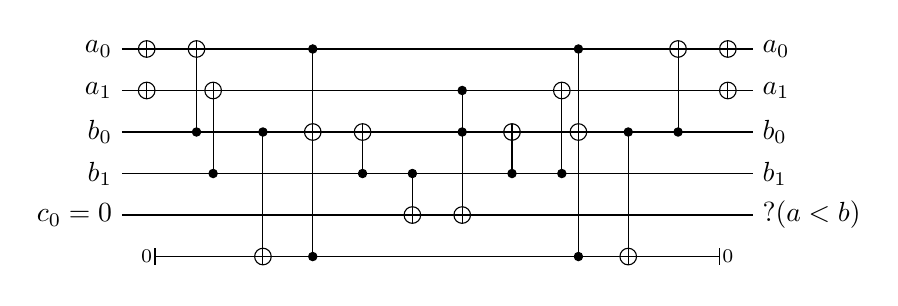
\begin{tikzpicture}[scale=1.000000,x=1pt,y=1pt]
\filldraw[color=white] (0.000000, -7.500000) rectangle (228.000000, 82.500000);
% Drawing wires
% Line 1: 0 W a_0 a_0
\draw[color=black] (0.000000,75.000000) -- (228.000000,75.000000);
\draw[color=black] (0.000000,75.000000) node[left] {$a_0$};
% Line 2: 1 W a_1 a_1
\draw[color=black] (0.000000,60.000000) -- (228.000000,60.000000);
\draw[color=black] (0.000000,60.000000) node[left] {$a_1$};
% Line 3: 2 W b_0 b_0
\draw[color=black] (0.000000,45.000000) -- (228.000000,45.000000);
\draw[color=black] (0.000000,45.000000) node[left] {$b_0$};
% Line 4: 3 W b_1 b_1
\draw[color=black] (0.000000,30.000000) -- (228.000000,30.000000);
\draw[color=black] (0.000000,30.000000) node[left] {$b_1$};
% Line 5: 4 W c_0=0 ?(a<b)
\draw[color=black] (0.000000,15.000000) -- (228.000000,15.000000);
\draw[color=black] (0.000000,15.000000) node[left] {$c_0=0$};
% Line 6: 7 W owire
\draw[color=black] (9.000000,0.000000) -- (219.000000,0.000000);
% Done with wires; drawing gates
% Line 7: +0
\begin{scope}
\draw[fill=white] (9.000000, 75.000000) circle(3.000000pt);
\clip (9.000000, 75.000000) circle(3.000000pt);
\draw (6.000000, 75.000000) -- (12.000000, 75.000000);
\draw (9.000000, 72.000000) -- (9.000000, 78.000000);
\end{scope}
% Line 8: +1
\begin{scope}
\draw[fill=white] (9.000000, 60.000000) circle(3.000000pt);
\clip (9.000000, 60.000000) circle(3.000000pt);
\draw (6.000000, 60.000000) -- (12.000000, 60.000000);
\draw (9.000000, 57.000000) -- (9.000000, 63.000000);
\end{scope}
% Line 9: 7 IN 0
\filldraw[color=white] (6.000000, -3.000000) rectangle (12.000000, 3.000000);
\draw (12.000000, -3.000000) -- (12.000000, 3.000000);
\draw (9.000000, 0.000000) node {$\scriptstyle{0}$};
% Line 10: +0 2
\draw (27.000000,75.000000) -- (27.000000,45.000000);
\begin{scope}
\draw[fill=white] (27.000000, 75.000000) circle(3.000000pt);
\clip (27.000000, 75.000000) circle(3.000000pt);
\draw (24.000000, 75.000000) -- (30.000000, 75.000000);
\draw (27.000000, 72.000000) -- (27.000000, 78.000000);
\end{scope}
\filldraw (27.000000, 45.000000) circle(1.500000pt);
% Line 13: +1 3
\draw (33.000000,60.000000) -- (33.000000,30.000000);
\begin{scope}
\draw[fill=white] (33.000000, 60.000000) circle(3.000000pt);
\clip (33.000000, 60.000000) circle(3.000000pt);
\draw (30.000000, 60.000000) -- (36.000000, 60.000000);
\draw (33.000000, 57.000000) -- (33.000000, 63.000000);
\end{scope}
\filldraw (33.000000, 30.000000) circle(1.500000pt);
% Line 11: +7 2
\draw (51.000000,45.000000) -- (51.000000,0.000000);
\begin{scope}
\draw[fill=white] (51.000000, 0.000000) circle(3.000000pt);
\clip (51.000000, 0.000000) circle(3.000000pt);
\draw (48.000000, 0.000000) -- (54.000000, 0.000000);
\draw (51.000000, -3.000000) -- (51.000000, 3.000000);
\end{scope}
\filldraw (51.000000, 45.000000) circle(1.500000pt);
% Line 12: +2 0 7
\draw (69.000000,75.000000) -- (69.000000,0.000000);
\begin{scope}
\draw[fill=white] (69.000000, 45.000000) circle(3.000000pt);
\clip (69.000000, 45.000000) circle(3.000000pt);
\draw (66.000000, 45.000000) -- (72.000000, 45.000000);
\draw (69.000000, 42.000000) -- (69.000000, 48.000000);
\end{scope}
\filldraw (69.000000, 75.000000) circle(1.500000pt);
\filldraw (69.000000, 0.000000) circle(1.500000pt);
% Line 14: +2 3
\draw (87.000000,45.000000) -- (87.000000,30.000000);
\begin{scope}
\draw[fill=white] (87.000000, 45.000000) circle(3.000000pt);
\clip (87.000000, 45.000000) circle(3.000000pt);
\draw (84.000000, 45.000000) -- (90.000000, 45.000000);
\draw (87.000000, 42.000000) -- (87.000000, 48.000000);
\end{scope}
\filldraw (87.000000, 30.000000) circle(1.500000pt);
% Line 15: +4 3
\draw (105.000000,30.000000) -- (105.000000,15.000000);
\begin{scope}
\draw[fill=white] (105.000000, 15.000000) circle(3.000000pt);
\clip (105.000000, 15.000000) circle(3.000000pt);
\draw (102.000000, 15.000000) -- (108.000000, 15.000000);
\draw (105.000000, 12.000000) -- (105.000000, 18.000000);
\end{scope}
\filldraw (105.000000, 30.000000) circle(1.500000pt);
% Line 16: +4 1 2
\draw (123.000000,60.000000) -- (123.000000,15.000000);
\begin{scope}
\draw[fill=white] (123.000000, 15.000000) circle(3.000000pt);
\clip (123.000000, 15.000000) circle(3.000000pt);
\draw (120.000000, 15.000000) -- (126.000000, 15.000000);
\draw (123.000000, 12.000000) -- (123.000000, 18.000000);
\end{scope}
\filldraw (123.000000, 60.000000) circle(1.500000pt);
\filldraw (123.000000, 45.000000) circle(1.500000pt);
% Line 17: +2 3
\draw (141.000000,45.000000) -- (141.000000,30.000000);
\begin{scope}
\draw[fill=white] (141.000000, 45.000000) circle(3.000000pt);
\clip (141.000000, 45.000000) circle(3.000000pt);
\draw (138.000000, 45.000000) -- (144.000000, 45.000000);
\draw (141.000000, 42.000000) -- (141.000000, 48.000000);
\end{scope}
\filldraw (141.000000, 30.000000) circle(1.500000pt);
% Line 18: +1 3
\draw (159.000000,60.000000) -- (159.000000,30.000000);
\begin{scope}
\draw[fill=white] (159.000000, 60.000000) circle(3.000000pt);
\clip (159.000000, 60.000000) circle(3.000000pt);
\draw (156.000000, 60.000000) -- (162.000000, 60.000000);
\draw (159.000000, 57.000000) -- (159.000000, 63.000000);
\end{scope}
\filldraw (159.000000, 30.000000) circle(1.500000pt);
% Line 19: +2 0 7
\draw (165.000000,75.000000) -- (165.000000,0.000000);
\begin{scope}
\draw[fill=white] (165.000000, 45.000000) circle(3.000000pt);
\clip (165.000000, 45.000000) circle(3.000000pt);
\draw (162.000000, 45.000000) -- (168.000000, 45.000000);
\draw (165.000000, 42.000000) -- (165.000000, 48.000000);
\end{scope}
\filldraw (165.000000, 75.000000) circle(1.500000pt);
\filldraw (165.000000, 0.000000) circle(1.500000pt);
% Line 20: +7 2
\draw (183.000000,45.000000) -- (183.000000,0.000000);
\begin{scope}
\draw[fill=white] (183.000000, 0.000000) circle(3.000000pt);
\clip (183.000000, 0.000000) circle(3.000000pt);
\draw (180.000000, 0.000000) -- (186.000000, 0.000000);
\draw (183.000000, -3.000000) -- (183.000000, 3.000000);
\end{scope}
\filldraw (183.000000, 45.000000) circle(1.500000pt);
% Line 21: +0 2
\draw (201.000000,75.000000) -- (201.000000,45.000000);
\begin{scope}
\draw[fill=white] (201.000000, 75.000000) circle(3.000000pt);
\clip (201.000000, 75.000000) circle(3.000000pt);
\draw (198.000000, 75.000000) -- (204.000000, 75.000000);
\draw (201.000000, 72.000000) -- (201.000000, 78.000000);
\end{scope}
\filldraw (201.000000, 45.000000) circle(1.500000pt);
% Line 22: TOUCH
% Line 23: 7 OUT 0
\filldraw[color=white] (216.000000, -3.000000) rectangle (222.000000, 3.000000);
\draw (216.000000, -3.000000) -- (216.000000, 3.000000);
\draw (219.000000, 0.000000) node {$\scriptstyle{0}$};
% Line 24: +0
\begin{scope}
\draw[fill=white] (219.000000, 75.000000) circle(3.000000pt);
\clip (219.000000, 75.000000) circle(3.000000pt);
\draw (216.000000, 75.000000) -- (222.000000, 75.000000);
\draw (219.000000, 72.000000) -- (219.000000, 78.000000);
\end{scope}
% Line 25: +1
\begin{scope}
\draw[fill=white] (219.000000, 60.000000) circle(3.000000pt);
\clip (219.000000, 60.000000) circle(3.000000pt);
\draw (216.000000, 60.000000) -- (222.000000, 60.000000);
\draw (219.000000, 57.000000) -- (219.000000, 63.000000);
\end{scope}
% Done with gates; drawing ending labels
\draw[color=black] (228.000000,75.000000) node[right] {$a_0$};
\draw[color=black] (228.000000,60.000000) node[right] {$a_1$};
\draw[color=black] (228.000000,45.000000) node[right] {$b_0$};
\draw[color=black] (228.000000,30.000000) node[right] {$b_1$};
\draw[color=black] (228.000000,15.000000) node[right] {$?(a<b)$};
% Done with ending labels; drawing cut lines and comments
% Done with comments
\end{tikzpicture}

\end{figure}

\SaveVerb{name}|Adder_CDKM|
\begin{figure}[ht]
\caption{\protect\UseVerb{name}}
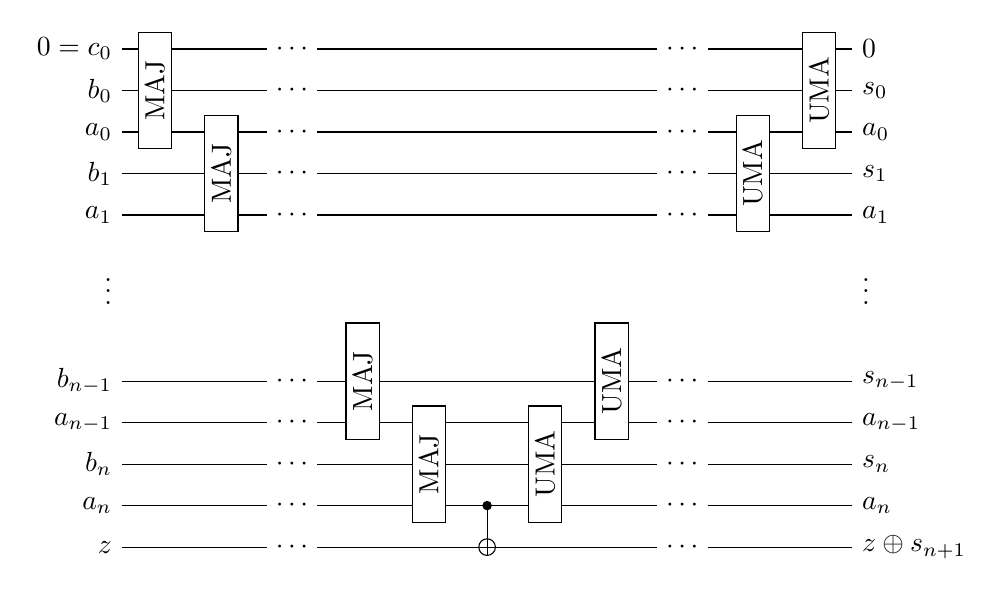
\begin{tikzpicture}[scale=1.000000,x=1pt,y=1pt]
\filldraw[color=white] (0.000000, -7.500000) rectangle (264.000000, 187.500000);
% Drawing wires
% Line 1: c0 W 0=c_0 0
\draw[color=black] (0.000000,180.000000) -- (264.000000,180.000000);
\draw[color=black] (0.000000,180.000000) node[left] {$0=c_0$};
% Line 2: b0 W b_0 s_0
\draw[color=black] (0.000000,165.000000) -- (264.000000,165.000000);
\draw[color=black] (0.000000,165.000000) node[left] {$b_0$};
% Line 3: a0 W a_0 a_0
\draw[color=black] (0.000000,150.000000) -- (264.000000,150.000000);
\draw[color=black] (0.000000,150.000000) node[left] {$a_0$};
% Line 4: b1 W b_1 s_1
\draw[color=black] (0.000000,135.000000) -- (264.000000,135.000000);
\draw[color=black] (0.000000,135.000000) node[left] {$b_1$};
% Line 5: a1 W a_1 a_1
\draw[color=black] (0.000000,120.000000) -- (264.000000,120.000000);
\draw[color=black] (0.000000,120.000000) node[left] {$a_1$};
% Line 6: z1 W color=white
\draw[color=white] (0.000000,105.000000) -- (264.000000,105.000000);
% Line 7: ... W
\draw[color=black] (0.000000,90.000000) node[anchor=mid east] {$\vdots$};
% Line 8: z2 W color=white
\draw[color=white] (0.000000,75.000000) -- (264.000000,75.000000);
% Line 9: bn1 W b_{n-1} s_{n-1}
\draw[color=black] (0.000000,60.000000) -- (264.000000,60.000000);
\draw[color=black] (0.000000,60.000000) node[left] {$b_{n-1}$};
% Line 10: an1 W a_{n-1} a_{n-1}
\draw[color=black] (0.000000,45.000000) -- (264.000000,45.000000);
\draw[color=black] (0.000000,45.000000) node[left] {$a_{n-1}$};
% Line 11: bn W b_n s_n
\draw[color=black] (0.000000,30.000000) -- (264.000000,30.000000);
\draw[color=black] (0.000000,30.000000) node[left] {$b_n$};
% Line 12: an W a_n a_n
\draw[color=black] (0.000000,15.000000) -- (264.000000,15.000000);
\draw[color=black] (0.000000,15.000000) node[left] {$a_n$};
% Line 13: z W z z\oplus{}s_{n+1}
\draw[color=black] (0.000000,0.000000) -- (264.000000,0.000000);
\draw[color=black] (0.000000,0.000000) node[left] {$z$};
% Done with wires; drawing gates
% Line 15: c0 b0 a0 G \rotatebox{90}{MAJ}
\draw (12.000000,180.000000) -- (12.000000,150.000000);
\begin{scope}
\draw[fill=white] (12.000000, 165.000000) +(-45.000000:8.485281pt and 29.698485pt) -- +(45.000000:8.485281pt and 29.698485pt) -- +(135.000000:8.485281pt and 29.698485pt) -- +(225.000000:8.485281pt and 29.698485pt) -- cycle;
\clip (12.000000, 165.000000) +(-45.000000:8.485281pt and 29.698485pt) -- +(45.000000:8.485281pt and 29.698485pt) -- +(135.000000:8.485281pt and 29.698485pt) -- +(225.000000:8.485281pt and 29.698485pt) -- cycle;
\draw (12.000000, 165.000000) node {\rotatebox{90}{MAJ}};
\end{scope}
% Line 16: a0 b1 a1 G \rotatebox{90}{MAJ}
\draw (36.000000,150.000000) -- (36.000000,120.000000);
\begin{scope}
\draw[fill=white] (36.000000, 135.000000) +(-45.000000:8.485281pt and 29.698485pt) -- +(45.000000:8.485281pt and 29.698485pt) -- +(135.000000:8.485281pt and 29.698485pt) -- +(225.000000:8.485281pt and 29.698485pt) -- cycle;
\clip (36.000000, 135.000000) +(-45.000000:8.485281pt and 29.698485pt) -- +(45.000000:8.485281pt and 29.698485pt) -- +(135.000000:8.485281pt and 29.698485pt) -- +(225.000000:8.485281pt and 29.698485pt) -- cycle;
\draw (36.000000, 135.000000) node {\rotatebox{90}{MAJ}};
\end{scope}
% Line 17: LABEL ...
\draw[color=black] (61.500000, 180.000000) node [fill=white] {$\cdots$};
\draw[color=black] (61.500000, 165.000000) node [fill=white] {$\cdots$};
\draw[color=black] (61.500000, 150.000000) node [fill=white] {$\cdots$};
\draw[color=black] (61.500000, 135.000000) node [fill=white] {$\cdots$};
\draw[color=black] (61.500000, 120.000000) node [fill=white] {$\cdots$};
\draw[color=white] (61.500000, 105.000000) node [fill=white] {$\cdots$};
\draw[color=white] (61.500000, 75.000000) node [fill=white] {$\cdots$};
\draw[color=black] (61.500000, 60.000000) node [fill=white] {$\cdots$};
\draw[color=black] (61.500000, 45.000000) node [fill=white] {$\cdots$};
\draw[color=black] (61.500000, 30.000000) node [fill=white] {$\cdots$};
\draw[color=black] (61.500000, 15.000000) node [fill=white] {$\cdots$};
\draw[color=black] (61.500000, 0.000000) node [fill=white] {$\cdots$};
% Line 18: z2 bn1 an1 G \rotatebox{90}{MAJ}
\draw (87.000000,75.000000) -- (87.000000,45.000000);
\begin{scope}
\draw[fill=white] (87.000000, 60.000000) +(-45.000000:8.485281pt and 29.698485pt) -- +(45.000000:8.485281pt and 29.698485pt) -- +(135.000000:8.485281pt and 29.698485pt) -- +(225.000000:8.485281pt and 29.698485pt) -- cycle;
\clip (87.000000, 60.000000) +(-45.000000:8.485281pt and 29.698485pt) -- +(45.000000:8.485281pt and 29.698485pt) -- +(135.000000:8.485281pt and 29.698485pt) -- +(225.000000:8.485281pt and 29.698485pt) -- cycle;
\draw (87.000000, 60.000000) node {\rotatebox{90}{MAJ}};
\end{scope}
% Line 19: an1 bn an G \rotatebox{90}{MAJ}
\draw (111.000000,45.000000) -- (111.000000,15.000000);
\begin{scope}
\draw[fill=white] (111.000000, 30.000000) +(-45.000000:8.485281pt and 29.698485pt) -- +(45.000000:8.485281pt and 29.698485pt) -- +(135.000000:8.485281pt and 29.698485pt) -- +(225.000000:8.485281pt and 29.698485pt) -- cycle;
\clip (111.000000, 30.000000) +(-45.000000:8.485281pt and 29.698485pt) -- +(45.000000:8.485281pt and 29.698485pt) -- +(135.000000:8.485281pt and 29.698485pt) -- +(225.000000:8.485281pt and 29.698485pt) -- cycle;
\draw (111.000000, 30.000000) node {\rotatebox{90}{MAJ}};
\end{scope}
% Line 20: +z an
\draw (132.000000,15.000000) -- (132.000000,0.000000);
\begin{scope}
\draw[fill=white] (132.000000, 0.000000) circle(3.000000pt);
\clip (132.000000, 0.000000) circle(3.000000pt);
\draw (129.000000, 0.000000) -- (135.000000, 0.000000);
\draw (132.000000, -3.000000) -- (132.000000, 3.000000);
\end{scope}
\filldraw (132.000000, 15.000000) circle(1.500000pt);
% Line 21: an1 bn an G \rotatebox{90}{UMA}
\draw (153.000000,45.000000) -- (153.000000,15.000000);
\begin{scope}
\draw[fill=white] (153.000000, 30.000000) +(-45.000000:8.485281pt and 29.698485pt) -- +(45.000000:8.485281pt and 29.698485pt) -- +(135.000000:8.485281pt and 29.698485pt) -- +(225.000000:8.485281pt and 29.698485pt) -- cycle;
\clip (153.000000, 30.000000) +(-45.000000:8.485281pt and 29.698485pt) -- +(45.000000:8.485281pt and 29.698485pt) -- +(135.000000:8.485281pt and 29.698485pt) -- +(225.000000:8.485281pt and 29.698485pt) -- cycle;
\draw (153.000000, 30.000000) node {\rotatebox{90}{UMA}};
\end{scope}
% Line 22: z2 bn1 an1 G \rotatebox{90}{UMA}
\draw (177.000000,75.000000) -- (177.000000,45.000000);
\begin{scope}
\draw[fill=white] (177.000000, 60.000000) +(-45.000000:8.485281pt and 29.698485pt) -- +(45.000000:8.485281pt and 29.698485pt) -- +(135.000000:8.485281pt and 29.698485pt) -- +(225.000000:8.485281pt and 29.698485pt) -- cycle;
\clip (177.000000, 60.000000) +(-45.000000:8.485281pt and 29.698485pt) -- +(45.000000:8.485281pt and 29.698485pt) -- +(135.000000:8.485281pt and 29.698485pt) -- +(225.000000:8.485281pt and 29.698485pt) -- cycle;
\draw (177.000000, 60.000000) node {\rotatebox{90}{UMA}};
\end{scope}
% Line 23: LABEL ...
\draw[color=black] (202.500000, 180.000000) node [fill=white] {$\cdots$};
\draw[color=black] (202.500000, 165.000000) node [fill=white] {$\cdots$};
\draw[color=black] (202.500000, 150.000000) node [fill=white] {$\cdots$};
\draw[color=black] (202.500000, 135.000000) node [fill=white] {$\cdots$};
\draw[color=black] (202.500000, 120.000000) node [fill=white] {$\cdots$};
\draw[color=white] (202.500000, 105.000000) node [fill=white] {$\cdots$};
\draw[color=white] (202.500000, 75.000000) node [fill=white] {$\cdots$};
\draw[color=black] (202.500000, 60.000000) node [fill=white] {$\cdots$};
\draw[color=black] (202.500000, 45.000000) node [fill=white] {$\cdots$};
\draw[color=black] (202.500000, 30.000000) node [fill=white] {$\cdots$};
\draw[color=black] (202.500000, 15.000000) node [fill=white] {$\cdots$};
\draw[color=black] (202.500000, 0.000000) node [fill=white] {$\cdots$};
% Line 24: a0 b1 a1 G \rotatebox{90}{UMA}
\draw (228.000000,150.000000) -- (228.000000,120.000000);
\begin{scope}
\draw[fill=white] (228.000000, 135.000000) +(-45.000000:8.485281pt and 29.698485pt) -- +(45.000000:8.485281pt and 29.698485pt) -- +(135.000000:8.485281pt and 29.698485pt) -- +(225.000000:8.485281pt and 29.698485pt) -- cycle;
\clip (228.000000, 135.000000) +(-45.000000:8.485281pt and 29.698485pt) -- +(45.000000:8.485281pt and 29.698485pt) -- +(135.000000:8.485281pt and 29.698485pt) -- +(225.000000:8.485281pt and 29.698485pt) -- cycle;
\draw (228.000000, 135.000000) node {\rotatebox{90}{UMA}};
\end{scope}
% Line 25: c0 b0 a0 G \rotatebox{90}{UMA}
\draw (252.000000,180.000000) -- (252.000000,150.000000);
\begin{scope}
\draw[fill=white] (252.000000, 165.000000) +(-45.000000:8.485281pt and 29.698485pt) -- +(45.000000:8.485281pt and 29.698485pt) -- +(135.000000:8.485281pt and 29.698485pt) -- +(225.000000:8.485281pt and 29.698485pt) -- cycle;
\clip (252.000000, 165.000000) +(-45.000000:8.485281pt and 29.698485pt) -- +(45.000000:8.485281pt and 29.698485pt) -- +(135.000000:8.485281pt and 29.698485pt) -- +(225.000000:8.485281pt and 29.698485pt) -- cycle;
\draw (252.000000, 165.000000) node {\rotatebox{90}{UMA}};
\end{scope}
% Done with gates; drawing ending labels
\draw[color=black] (264.000000,180.000000) node[right] {$0$};
\draw[color=black] (264.000000,165.000000) node[right] {$s_0$};
\draw[color=black] (264.000000,150.000000) node[right] {$a_0$};
\draw[color=black] (264.000000,135.000000) node[right] {$s_1$};
\draw[color=black] (264.000000,120.000000) node[right] {$a_1$};
\draw[color=black] (264.000000,90.000000) node[anchor=mid west] {$\vdots$};
\draw[color=black] (264.000000,60.000000) node[right] {$s_{n-1}$};
\draw[color=black] (264.000000,45.000000) node[right] {$a_{n-1}$};
\draw[color=black] (264.000000,30.000000) node[right] {$s_n$};
\draw[color=black] (264.000000,15.000000) node[right] {$a_n$};
\draw[color=black] (264.000000,0.000000) node[right] {$z\oplus{}s_{n+1}$};
% Done with ending labels; drawing cut lines and comments
% Done with comments
\end{tikzpicture}

\end{figure}

\SaveVerb{name}|Adder_CDKM_MAJ|
\begin{figure}[ht]
\caption{\protect\UseVerb{name}}
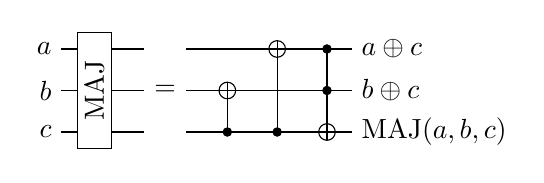
\begin{tikzpicture}[scale=1.000000,x=1pt,y=1pt]
\filldraw[color=white] (0.000000, -7.500000) rectangle (105.000000, 37.500000);
% Drawing wires
% Line 1: a W a a\oplus{c}
\draw[color=black] (0.000000,30.000000) -- (105.000000,30.000000);
\draw[color=black] (0.000000,30.000000) node[left] {$a$};
% Line 2: b W b b\oplus{c}
\draw[color=black] (0.000000,15.000000) -- (105.000000,15.000000);
\draw[color=black] (0.000000,15.000000) node[left] {$b$};
% Line 3: c W c \mbox{MAJ}(a,b,c)
\draw[color=black] (0.000000,0.000000) -- (105.000000,0.000000);
\draw[color=black] (0.000000,0.000000) node[left] {$c$};
% Done with wires; drawing gates
% Line 5: a b c G \rotatebox{90}{MAJ}
\draw (12.000000,30.000000) -- (12.000000,0.000000);
\begin{scope}
\draw[fill=white] (12.000000, 15.000000) +(-45.000000:8.485281pt and 29.698485pt) -- +(45.000000:8.485281pt and 29.698485pt) -- +(135.000000:8.485281pt and 29.698485pt) -- +(225.000000:8.485281pt and 29.698485pt) -- cycle;
\clip (12.000000, 15.000000) +(-45.000000:8.485281pt and 29.698485pt) -- +(45.000000:8.485281pt and 29.698485pt) -- +(135.000000:8.485281pt and 29.698485pt) -- +(225.000000:8.485281pt and 29.698485pt) -- cycle;
\draw (12.000000, 15.000000) node {\rotatebox{90}{MAJ}};
\end{scope}
% Line 6: =
\draw[fill=white,color=white] (30.000000, -6.000000) rectangle (45.000000, 36.000000);
\draw (37.500000, 15.000000) node {$=$};
% Line 7: +b c
\draw (60.000000,15.000000) -- (60.000000,0.000000);
\begin{scope}
\draw[fill=white] (60.000000, 15.000000) circle(3.000000pt);
\clip (60.000000, 15.000000) circle(3.000000pt);
\draw (57.000000, 15.000000) -- (63.000000, 15.000000);
\draw (60.000000, 12.000000) -- (60.000000, 18.000000);
\end{scope}
\filldraw (60.000000, 0.000000) circle(1.500000pt);
% Line 8: +a c
\draw (78.000000,30.000000) -- (78.000000,0.000000);
\begin{scope}
\draw[fill=white] (78.000000, 30.000000) circle(3.000000pt);
\clip (78.000000, 30.000000) circle(3.000000pt);
\draw (75.000000, 30.000000) -- (81.000000, 30.000000);
\draw (78.000000, 27.000000) -- (78.000000, 33.000000);
\end{scope}
\filldraw (78.000000, 0.000000) circle(1.500000pt);
% Line 9: a b +c
\draw (96.000000,30.000000) -- (96.000000,0.000000);
\filldraw (96.000000, 30.000000) circle(1.500000pt);
\filldraw (96.000000, 15.000000) circle(1.500000pt);
\begin{scope}
\draw[fill=white] (96.000000, 0.000000) circle(3.000000pt);
\clip (96.000000, 0.000000) circle(3.000000pt);
\draw (93.000000, 0.000000) -- (99.000000, 0.000000);
\draw (96.000000, -3.000000) -- (96.000000, 3.000000);
\end{scope}
% Done with gates; drawing ending labels
\draw[color=black] (105.000000,30.000000) node[right] {$a\oplus{c}$};
\draw[color=black] (105.000000,15.000000) node[right] {$b\oplus{c}$};
\draw[color=black] (105.000000,0.000000) node[right] {$\mbox{MAJ}(a,b,c)$};
% Done with ending labels; drawing cut lines and comments
% Done with comments
\end{tikzpicture}

\end{figure}

\SaveVerb{name}|Adder_CDKM_UMA|
\begin{figure}[ht]
\caption{\protect\UseVerb{name}}
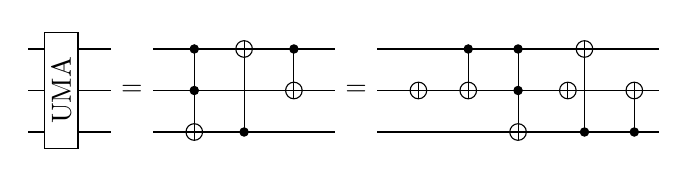
\begin{tikzpicture}[scale=1.000000,x=1pt,y=1pt]
\filldraw[color=white] (0.000000, -7.500000) rectangle (228.000000, 37.500000);
% Drawing wires
% Line 1: a W #a\oplus{c}
\draw[color=black] (0.000000,30.000000) -- (228.000000,30.000000);
% Line 2: b W #b\oplus{c}
\draw[color=black] (0.000000,15.000000) -- (228.000000,15.000000);
% Line 3: c W #\mbox{MAJ}(a,b,c)
\draw[color=black] (0.000000,0.000000) -- (228.000000,0.000000);
% Done with wires; drawing gates
% Line 5: a b c G \rotatebox{90}{UMA}
\draw (12.000000,30.000000) -- (12.000000,0.000000);
\begin{scope}
\draw[fill=white] (12.000000, 15.000000) +(-45.000000:8.485281pt and 29.698485pt) -- +(45.000000:8.485281pt and 29.698485pt) -- +(135.000000:8.485281pt and 29.698485pt) -- +(225.000000:8.485281pt and 29.698485pt) -- cycle;
\clip (12.000000, 15.000000) +(-45.000000:8.485281pt and 29.698485pt) -- +(45.000000:8.485281pt and 29.698485pt) -- +(135.000000:8.485281pt and 29.698485pt) -- +(225.000000:8.485281pt and 29.698485pt) -- cycle;
\draw (12.000000, 15.000000) node {\rotatebox{90}{UMA}};
\end{scope}
% Line 6: =
\draw[fill=white,color=white] (30.000000, -6.000000) rectangle (45.000000, 36.000000);
\draw (37.500000, 15.000000) node {$=$};
% Line 7: +c a b
\draw (60.000000,30.000000) -- (60.000000,0.000000);
\begin{scope}
\draw[fill=white] (60.000000, 0.000000) circle(3.000000pt);
\clip (60.000000, 0.000000) circle(3.000000pt);
\draw (57.000000, 0.000000) -- (63.000000, 0.000000);
\draw (60.000000, -3.000000) -- (60.000000, 3.000000);
\end{scope}
\filldraw (60.000000, 30.000000) circle(1.500000pt);
\filldraw (60.000000, 15.000000) circle(1.500000pt);
% Line 8: +a c
\draw (78.000000,30.000000) -- (78.000000,0.000000);
\begin{scope}
\draw[fill=white] (78.000000, 30.000000) circle(3.000000pt);
\clip (78.000000, 30.000000) circle(3.000000pt);
\draw (75.000000, 30.000000) -- (81.000000, 30.000000);
\draw (78.000000, 27.000000) -- (78.000000, 33.000000);
\end{scope}
\filldraw (78.000000, 0.000000) circle(1.500000pt);
% Line 9: +b a
\draw (96.000000,30.000000) -- (96.000000,15.000000);
\begin{scope}
\draw[fill=white] (96.000000, 15.000000) circle(3.000000pt);
\clip (96.000000, 15.000000) circle(3.000000pt);
\draw (93.000000, 15.000000) -- (99.000000, 15.000000);
\draw (96.000000, 12.000000) -- (96.000000, 18.000000);
\end{scope}
\filldraw (96.000000, 30.000000) circle(1.500000pt);
% Line 10: =
\draw[fill=white,color=white] (111.000000, -6.000000) rectangle (126.000000, 36.000000);
\draw (118.500000, 15.000000) node {$=$};
% Line 11: +b
\begin{scope}
\draw[fill=white] (141.000000, 15.000000) circle(3.000000pt);
\clip (141.000000, 15.000000) circle(3.000000pt);
\draw (138.000000, 15.000000) -- (144.000000, 15.000000);
\draw (141.000000, 12.000000) -- (141.000000, 18.000000);
\end{scope}
% Line 12: +b a
\draw (159.000000,30.000000) -- (159.000000,15.000000);
\begin{scope}
\draw[fill=white] (159.000000, 15.000000) circle(3.000000pt);
\clip (159.000000, 15.000000) circle(3.000000pt);
\draw (156.000000, 15.000000) -- (162.000000, 15.000000);
\draw (159.000000, 12.000000) -- (159.000000, 18.000000);
\end{scope}
\filldraw (159.000000, 30.000000) circle(1.500000pt);
% Line 13: +c a b
\draw (177.000000,30.000000) -- (177.000000,0.000000);
\begin{scope}
\draw[fill=white] (177.000000, 0.000000) circle(3.000000pt);
\clip (177.000000, 0.000000) circle(3.000000pt);
\draw (174.000000, 0.000000) -- (180.000000, 0.000000);
\draw (177.000000, -3.000000) -- (177.000000, 3.000000);
\end{scope}
\filldraw (177.000000, 30.000000) circle(1.500000pt);
\filldraw (177.000000, 15.000000) circle(1.500000pt);
% Line 14: +b
\begin{scope}
\draw[fill=white] (195.000000, 15.000000) circle(3.000000pt);
\clip (195.000000, 15.000000) circle(3.000000pt);
\draw (192.000000, 15.000000) -- (198.000000, 15.000000);
\draw (195.000000, 12.000000) -- (195.000000, 18.000000);
\end{scope}
% Line 15: +a c
\draw (201.000000,30.000000) -- (201.000000,0.000000);
\begin{scope}
\draw[fill=white] (201.000000, 30.000000) circle(3.000000pt);
\clip (201.000000, 30.000000) circle(3.000000pt);
\draw (198.000000, 30.000000) -- (204.000000, 30.000000);
\draw (201.000000, 27.000000) -- (201.000000, 33.000000);
\end{scope}
\filldraw (201.000000, 0.000000) circle(1.500000pt);
% Line 16: +b c
\draw (219.000000,15.000000) -- (219.000000,0.000000);
\begin{scope}
\draw[fill=white] (219.000000, 15.000000) circle(3.000000pt);
\clip (219.000000, 15.000000) circle(3.000000pt);
\draw (216.000000, 15.000000) -- (222.000000, 15.000000);
\draw (219.000000, 12.000000) -- (219.000000, 18.000000);
\end{scope}
\filldraw (219.000000, 0.000000) circle(1.500000pt);
% Done with gates; drawing ending labels
% Done with ending labels; drawing cut lines and comments
% Done with comments
\end{tikzpicture}

\end{figure}

\SaveVerb{name}|Adder_VBE|
\begin{figure}[ht]
\caption{\protect\UseVerb{name}}
%! \usepackage{hyperref}
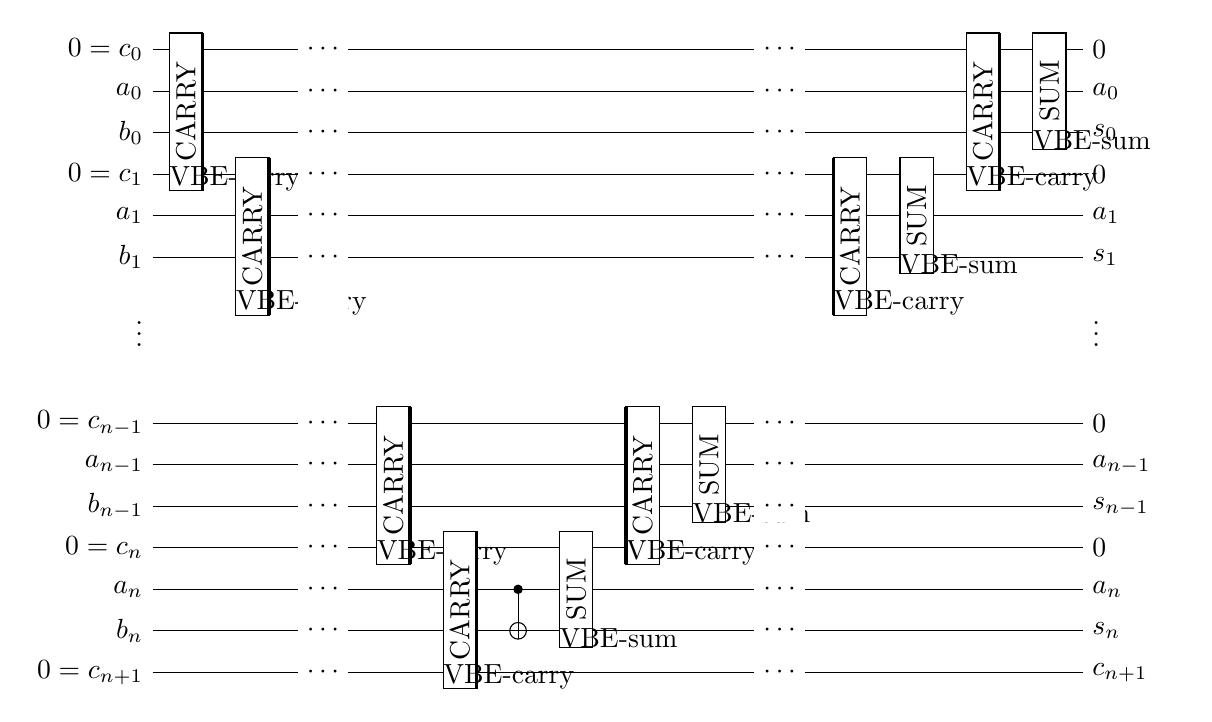
\begin{tikzpicture}[scale=1.000000,x=1pt,y=1pt]
\filldraw[color=white] (0.000000, -7.500000) rectangle (336.000000, 232.500000);
% Drawing wires
% Line 1: c0 W 0=c_0 0
\draw[color=black] (0.000000,225.000000) -- (336.000000,225.000000);
\draw[color=black] (0.000000,225.000000) node[left] {$0=c_0$};
% Line 2: a0 W a_0 a_0
\draw[color=black] (0.000000,210.000000) -- (336.000000,210.000000);
\draw[color=black] (0.000000,210.000000) node[left] {$a_0$};
% Line 3: b0 W b_0 s_0
\draw[color=black] (0.000000,195.000000) -- (336.000000,195.000000);
\draw[color=black] (0.000000,195.000000) node[left] {$b_0$};
% Line 4: c1 W 0=c_1 0
\draw[color=black] (0.000000,180.000000) -- (336.000000,180.000000);
\draw[color=black] (0.000000,180.000000) node[left] {$0=c_1$};
% Line 5: a1 W a_1 a_1
\draw[color=black] (0.000000,165.000000) -- (336.000000,165.000000);
\draw[color=black] (0.000000,165.000000) node[left] {$a_1$};
% Line 6: b1 W b_1 s_1
\draw[color=black] (0.000000,150.000000) -- (336.000000,150.000000);
\draw[color=black] (0.000000,150.000000) node[left] {$b_1$};
% Line 7: z1 W color=white
\draw[color=white] (0.000000,135.000000) -- (336.000000,135.000000);
% Line 8: ... W
\draw[color=black] (0.000000,120.000000) node[anchor=mid east] {$\vdots$};
% Line 9: z2 W color=white
\draw[color=white] (0.000000,105.000000) -- (336.000000,105.000000);
% Line 10: cn1 W 0=c_{n-1} 0
\draw[color=black] (0.000000,90.000000) -- (336.000000,90.000000);
\draw[color=black] (0.000000,90.000000) node[left] {$0=c_{n-1}$};
% Line 11: an1 W a_{n-1} a_{n-1}
\draw[color=black] (0.000000,75.000000) -- (336.000000,75.000000);
\draw[color=black] (0.000000,75.000000) node[left] {$a_{n-1}$};
% Line 12: bn1 W b_{n-1} s_{n-1}
\draw[color=black] (0.000000,60.000000) -- (336.000000,60.000000);
\draw[color=black] (0.000000,60.000000) node[left] {$b_{n-1}$};
% Line 13: cn W 0=c_n 0
\draw[color=black] (0.000000,45.000000) -- (336.000000,45.000000);
\draw[color=black] (0.000000,45.000000) node[left] {$0=c_n$};
% Line 14: an W a_n a_n
\draw[color=black] (0.000000,30.000000) -- (336.000000,30.000000);
\draw[color=black] (0.000000,30.000000) node[left] {$a_n$};
% Line 15: bn W b_n s_n
\draw[color=black] (0.000000,15.000000) -- (336.000000,15.000000);
\draw[color=black] (0.000000,15.000000) node[left] {$b_n$};
% Line 16: cnc W 0=c_{n+1} c_{n+1}
\draw[color=black] (0.000000,0.000000) -- (336.000000,0.000000);
\draw[color=black] (0.000000,0.000000) node[left] {$0=c_{n+1}$};
% Done with wires; drawing gates
% Line 18: c0 a0 b0 c1  G| \rotatebox{90}{CARRY} hyperlink=VBE-carry
\draw (12.000000,225.000000) -- (12.000000,180.000000);
\begin{scope}
\draw[fill=white] (12.000000, 202.500000) +(-45.000000:8.485281pt and 40.305087pt) -- +(45.000000:8.485281pt and 40.305087pt) -- +(135.000000:8.485281pt and 40.305087pt) -- +(225.000000:8.485281pt and 40.305087pt) -- cycle;
\draw[very thick,solid] (12.000000, 202.500000) +(-45.000000:8.485281pt and 40.305087pt) -- +(45.000000:8.485281pt and 40.305087pt);
\clip (12.000000, 202.500000) +(-45.000000:8.485281pt and 40.305087pt) -- +(45.000000:8.485281pt and 40.305087pt) -- +(135.000000:8.485281pt and 40.305087pt) -- +(225.000000:8.485281pt and 40.305087pt) -- cycle;
\draw (12.000000, 202.500000) node {\rotatebox{90}{CARRY}};
\end{scope}
\draw (6.000000,174.000000) node[inner sep=0pt, outer sep=0pt, anchor=south west] {\hyperlink{VBE-carry}{\phantom{\rule{12.000000pt}{57.000000pt}}}};
% Line 19: c1 a1 b1 z1  G| \rotatebox{90}{CARRY} hyperlink=VBE-carry
\draw (36.000000,180.000000) -- (36.000000,135.000000);
\begin{scope}
\draw[fill=white] (36.000000, 157.500000) +(-45.000000:8.485281pt and 40.305087pt) -- +(45.000000:8.485281pt and 40.305087pt) -- +(135.000000:8.485281pt and 40.305087pt) -- +(225.000000:8.485281pt and 40.305087pt) -- cycle;
\draw[very thick,solid] (36.000000, 157.500000) +(-45.000000:8.485281pt and 40.305087pt) -- +(45.000000:8.485281pt and 40.305087pt);
\clip (36.000000, 157.500000) +(-45.000000:8.485281pt and 40.305087pt) -- +(45.000000:8.485281pt and 40.305087pt) -- +(135.000000:8.485281pt and 40.305087pt) -- +(225.000000:8.485281pt and 40.305087pt) -- cycle;
\draw (36.000000, 157.500000) node {\rotatebox{90}{CARRY}};
\end{scope}
\draw (30.000000,129.000000) node[inner sep=0pt, outer sep=0pt, anchor=south west] {\hyperlink{VBE-carry}{\phantom{\rule{12.000000pt}{57.000000pt}}}};
% Line 20: LABEL ...
\draw[color=black] (61.500000, 225.000000) node [fill=white] {$\cdots$};
\draw[color=black] (61.500000, 210.000000) node [fill=white] {$\cdots$};
\draw[color=black] (61.500000, 195.000000) node [fill=white] {$\cdots$};
\draw[color=black] (61.500000, 180.000000) node [fill=white] {$\cdots$};
\draw[color=black] (61.500000, 165.000000) node [fill=white] {$\cdots$};
\draw[color=black] (61.500000, 150.000000) node [fill=white] {$\cdots$};
\draw[color=white] (61.500000, 135.000000) node [fill=white] {$\cdots$};
\draw[color=white] (61.500000, 105.000000) node [fill=white] {$\cdots$};
\draw[color=black] (61.500000, 90.000000) node [fill=white] {$\cdots$};
\draw[color=black] (61.500000, 75.000000) node [fill=white] {$\cdots$};
\draw[color=black] (61.500000, 60.000000) node [fill=white] {$\cdots$};
\draw[color=black] (61.500000, 45.000000) node [fill=white] {$\cdots$};
\draw[color=black] (61.500000, 30.000000) node [fill=white] {$\cdots$};
\draw[color=black] (61.500000, 15.000000) node [fill=white] {$\cdots$};
\draw[color=black] (61.500000, 0.000000) node [fill=white] {$\cdots$};
% Line 21: cn1 an1 bn1 cn  G| \rotatebox{90}{CARRY} hyperlink=VBE-carry
\draw (87.000000,90.000000) -- (87.000000,45.000000);
\begin{scope}
\draw[fill=white] (87.000000, 67.500000) +(-45.000000:8.485281pt and 40.305087pt) -- +(45.000000:8.485281pt and 40.305087pt) -- +(135.000000:8.485281pt and 40.305087pt) -- +(225.000000:8.485281pt and 40.305087pt) -- cycle;
\draw[very thick,solid] (87.000000, 67.500000) +(-45.000000:8.485281pt and 40.305087pt) -- +(45.000000:8.485281pt and 40.305087pt);
\clip (87.000000, 67.500000) +(-45.000000:8.485281pt and 40.305087pt) -- +(45.000000:8.485281pt and 40.305087pt) -- +(135.000000:8.485281pt and 40.305087pt) -- +(225.000000:8.485281pt and 40.305087pt) -- cycle;
\draw (87.000000, 67.500000) node {\rotatebox{90}{CARRY}};
\end{scope}
\draw (81.000000,39.000000) node[inner sep=0pt, outer sep=0pt, anchor=south west] {\hyperlink{VBE-carry}{\phantom{\rule{12.000000pt}{57.000000pt}}}};
% Line 22: cn an bn cnc  G| \rotatebox{90}{CARRY} hyperlink=VBE-carry
\draw (111.000000,45.000000) -- (111.000000,0.000000);
\begin{scope}
\draw[fill=white] (111.000000, 22.500000) +(-45.000000:8.485281pt and 40.305087pt) -- +(45.000000:8.485281pt and 40.305087pt) -- +(135.000000:8.485281pt and 40.305087pt) -- +(225.000000:8.485281pt and 40.305087pt) -- cycle;
\draw[very thick,solid] (111.000000, 22.500000) +(-45.000000:8.485281pt and 40.305087pt) -- +(45.000000:8.485281pt and 40.305087pt);
\clip (111.000000, 22.500000) +(-45.000000:8.485281pt and 40.305087pt) -- +(45.000000:8.485281pt and 40.305087pt) -- +(135.000000:8.485281pt and 40.305087pt) -- +(225.000000:8.485281pt and 40.305087pt) -- cycle;
\draw (111.000000, 22.500000) node {\rotatebox{90}{CARRY}};
\end{scope}
\draw (105.000000,-6.000000) node[inner sep=0pt, outer sep=0pt, anchor=south west] {\hyperlink{VBE-carry}{\phantom{\rule{12.000000pt}{57.000000pt}}}};
% Line 23: +bn an
\draw (132.000000,30.000000) -- (132.000000,15.000000);
\begin{scope}
\draw[fill=white] (132.000000, 15.000000) circle(3.000000pt);
\clip (132.000000, 15.000000) circle(3.000000pt);
\draw (129.000000, 15.000000) -- (135.000000, 15.000000);
\draw (132.000000, 12.000000) -- (132.000000, 18.000000);
\end{scope}
\filldraw (132.000000, 30.000000) circle(1.500000pt);
% Line 24: cn an bn  G \rotatebox{90}{SUM} hyperlink=VBE-sum
\draw (153.000000,45.000000) -- (153.000000,15.000000);
\begin{scope}
\draw[fill=white] (153.000000, 30.000000) +(-45.000000:8.485281pt and 29.698485pt) -- +(45.000000:8.485281pt and 29.698485pt) -- +(135.000000:8.485281pt and 29.698485pt) -- +(225.000000:8.485281pt and 29.698485pt) -- cycle;
\clip (153.000000, 30.000000) +(-45.000000:8.485281pt and 29.698485pt) -- +(45.000000:8.485281pt and 29.698485pt) -- +(135.000000:8.485281pt and 29.698485pt) -- +(225.000000:8.485281pt and 29.698485pt) -- cycle;
\draw (153.000000, 30.000000) node {\rotatebox{90}{SUM}};
\end{scope}
\draw (147.000000,9.000000) node[inner sep=0pt, outer sep=0pt, anchor=south west] {\hyperlink{VBE-sum}{\phantom{\rule{12.000000pt}{42.000000pt}}}};
% Line 25: cn1 an1 bn1 cn  |G \rotatebox{90}{CARRY} hyperlink=VBE-carry
\draw (177.000000,90.000000) -- (177.000000,45.000000);
\begin{scope}
\draw[fill=white] (177.000000, 67.500000) +(-45.000000:8.485281pt and 40.305087pt) -- +(45.000000:8.485281pt and 40.305087pt) -- +(135.000000:8.485281pt and 40.305087pt) -- +(225.000000:8.485281pt and 40.305087pt) -- cycle;
\draw[very thick,solid] (177.000000, 67.500000) +(135.000000:8.485281pt and 40.305087pt) -- +(225.000000:8.485281pt and 40.305087pt);
\clip (177.000000, 67.500000) +(-45.000000:8.485281pt and 40.305087pt) -- +(45.000000:8.485281pt and 40.305087pt) -- +(135.000000:8.485281pt and 40.305087pt) -- +(225.000000:8.485281pt and 40.305087pt) -- cycle;
\draw (177.000000, 67.500000) node {\rotatebox{90}{CARRY}};
\end{scope}
\draw (171.000000,39.000000) node[inner sep=0pt, outer sep=0pt, anchor=south west] {\hyperlink{VBE-carry}{\phantom{\rule{12.000000pt}{57.000000pt}}}};
% Line 26: cn1 an1 bn1  G \rotatebox{90}{SUM} hyperlink=VBE-sum
\draw (201.000000,90.000000) -- (201.000000,60.000000);
\begin{scope}
\draw[fill=white] (201.000000, 75.000000) +(-45.000000:8.485281pt and 29.698485pt) -- +(45.000000:8.485281pt and 29.698485pt) -- +(135.000000:8.485281pt and 29.698485pt) -- +(225.000000:8.485281pt and 29.698485pt) -- cycle;
\clip (201.000000, 75.000000) +(-45.000000:8.485281pt and 29.698485pt) -- +(45.000000:8.485281pt and 29.698485pt) -- +(135.000000:8.485281pt and 29.698485pt) -- +(225.000000:8.485281pt and 29.698485pt) -- cycle;
\draw (201.000000, 75.000000) node {\rotatebox{90}{SUM}};
\end{scope}
\draw (195.000000,54.000000) node[inner sep=0pt, outer sep=0pt, anchor=south west] {\hyperlink{VBE-sum}{\phantom{\rule{12.000000pt}{42.000000pt}}}};
% Line 27: LABEL ...
\draw[color=black] (226.500000, 225.000000) node [fill=white] {$\cdots$};
\draw[color=black] (226.500000, 210.000000) node [fill=white] {$\cdots$};
\draw[color=black] (226.500000, 195.000000) node [fill=white] {$\cdots$};
\draw[color=black] (226.500000, 180.000000) node [fill=white] {$\cdots$};
\draw[color=black] (226.500000, 165.000000) node [fill=white] {$\cdots$};
\draw[color=black] (226.500000, 150.000000) node [fill=white] {$\cdots$};
\draw[color=white] (226.500000, 135.000000) node [fill=white] {$\cdots$};
\draw[color=white] (226.500000, 105.000000) node [fill=white] {$\cdots$};
\draw[color=black] (226.500000, 90.000000) node [fill=white] {$\cdots$};
\draw[color=black] (226.500000, 75.000000) node [fill=white] {$\cdots$};
\draw[color=black] (226.500000, 60.000000) node [fill=white] {$\cdots$};
\draw[color=black] (226.500000, 45.000000) node [fill=white] {$\cdots$};
\draw[color=black] (226.500000, 30.000000) node [fill=white] {$\cdots$};
\draw[color=black] (226.500000, 15.000000) node [fill=white] {$\cdots$};
\draw[color=black] (226.500000, 0.000000) node [fill=white] {$\cdots$};
% Line 28: c1 a1 b1 z1  |G \rotatebox{90}{CARRY} hyperlink=VBE-carry
\draw (252.000000,180.000000) -- (252.000000,135.000000);
\begin{scope}
\draw[fill=white] (252.000000, 157.500000) +(-45.000000:8.485281pt and 40.305087pt) -- +(45.000000:8.485281pt and 40.305087pt) -- +(135.000000:8.485281pt and 40.305087pt) -- +(225.000000:8.485281pt and 40.305087pt) -- cycle;
\draw[very thick,solid] (252.000000, 157.500000) +(135.000000:8.485281pt and 40.305087pt) -- +(225.000000:8.485281pt and 40.305087pt);
\clip (252.000000, 157.500000) +(-45.000000:8.485281pt and 40.305087pt) -- +(45.000000:8.485281pt and 40.305087pt) -- +(135.000000:8.485281pt and 40.305087pt) -- +(225.000000:8.485281pt and 40.305087pt) -- cycle;
\draw (252.000000, 157.500000) node {\rotatebox{90}{CARRY}};
\end{scope}
\draw (246.000000,129.000000) node[inner sep=0pt, outer sep=0pt, anchor=south west] {\hyperlink{VBE-carry}{\phantom{\rule{12.000000pt}{57.000000pt}}}};
% Line 29: c1 a1 b1  G \rotatebox{90}{SUM} hyperlink=VBE-sum
\draw (276.000000,180.000000) -- (276.000000,150.000000);
\begin{scope}
\draw[fill=white] (276.000000, 165.000000) +(-45.000000:8.485281pt and 29.698485pt) -- +(45.000000:8.485281pt and 29.698485pt) -- +(135.000000:8.485281pt and 29.698485pt) -- +(225.000000:8.485281pt and 29.698485pt) -- cycle;
\clip (276.000000, 165.000000) +(-45.000000:8.485281pt and 29.698485pt) -- +(45.000000:8.485281pt and 29.698485pt) -- +(135.000000:8.485281pt and 29.698485pt) -- +(225.000000:8.485281pt and 29.698485pt) -- cycle;
\draw (276.000000, 165.000000) node {\rotatebox{90}{SUM}};
\end{scope}
\draw (270.000000,144.000000) node[inner sep=0pt, outer sep=0pt, anchor=south west] {\hyperlink{VBE-sum}{\phantom{\rule{12.000000pt}{42.000000pt}}}};
% Line 30: c0 a0 b0 c1  G| \rotatebox{90}{CARRY} hyperlink=VBE-carry
\draw (300.000000,225.000000) -- (300.000000,180.000000);
\begin{scope}
\draw[fill=white] (300.000000, 202.500000) +(-45.000000:8.485281pt and 40.305087pt) -- +(45.000000:8.485281pt and 40.305087pt) -- +(135.000000:8.485281pt and 40.305087pt) -- +(225.000000:8.485281pt and 40.305087pt) -- cycle;
\draw[very thick,solid] (300.000000, 202.500000) +(-45.000000:8.485281pt and 40.305087pt) -- +(45.000000:8.485281pt and 40.305087pt);
\clip (300.000000, 202.500000) +(-45.000000:8.485281pt and 40.305087pt) -- +(45.000000:8.485281pt and 40.305087pt) -- +(135.000000:8.485281pt and 40.305087pt) -- +(225.000000:8.485281pt and 40.305087pt) -- cycle;
\draw (300.000000, 202.500000) node {\rotatebox{90}{CARRY}};
\end{scope}
\draw (294.000000,174.000000) node[inner sep=0pt, outer sep=0pt, anchor=south west] {\hyperlink{VBE-carry}{\phantom{\rule{12.000000pt}{57.000000pt}}}};
% Line 31: c0 a0 b0  G \rotatebox{90}{SUM} hyperlink=VBE-sum
\draw (324.000000,225.000000) -- (324.000000,195.000000);
\begin{scope}
\draw[fill=white] (324.000000, 210.000000) +(-45.000000:8.485281pt and 29.698485pt) -- +(45.000000:8.485281pt and 29.698485pt) -- +(135.000000:8.485281pt and 29.698485pt) -- +(225.000000:8.485281pt and 29.698485pt) -- cycle;
\clip (324.000000, 210.000000) +(-45.000000:8.485281pt and 29.698485pt) -- +(45.000000:8.485281pt and 29.698485pt) -- +(135.000000:8.485281pt and 29.698485pt) -- +(225.000000:8.485281pt and 29.698485pt) -- cycle;
\draw (324.000000, 210.000000) node {\rotatebox{90}{SUM}};
\end{scope}
\draw (318.000000,189.000000) node[inner sep=0pt, outer sep=0pt, anchor=south west] {\hyperlink{VBE-sum}{\phantom{\rule{12.000000pt}{42.000000pt}}}};
% Done with gates; drawing ending labels
\draw[color=black] (336.000000,225.000000) node[right] {$0$};
\draw[color=black] (336.000000,210.000000) node[right] {$a_0$};
\draw[color=black] (336.000000,195.000000) node[right] {$s_0$};
\draw[color=black] (336.000000,180.000000) node[right] {$0$};
\draw[color=black] (336.000000,165.000000) node[right] {$a_1$};
\draw[color=black] (336.000000,150.000000) node[right] {$s_1$};
\draw[color=black] (336.000000,120.000000) node[anchor=mid west] {$\vdots$};
\draw[color=black] (336.000000,90.000000) node[right] {$0$};
\draw[color=black] (336.000000,75.000000) node[right] {$a_{n-1}$};
\draw[color=black] (336.000000,60.000000) node[right] {$s_{n-1}$};
\draw[color=black] (336.000000,45.000000) node[right] {$0$};
\draw[color=black] (336.000000,30.000000) node[right] {$a_n$};
\draw[color=black] (336.000000,15.000000) node[right] {$s_n$};
\draw[color=black] (336.000000,0.000000) node[right] {$c_{n+1}$};
% Done with ending labels; drawing cut lines and comments
% Done with comments
\end{tikzpicture}

\end{figure}

\SaveVerb{name}|Adder_VBE_Carry|
\begin{figure}[ht]
\caption{\protect\UseVerb{name}}
%! \usepackage{hyperref}
\hypertarget{VBE-carry}{}
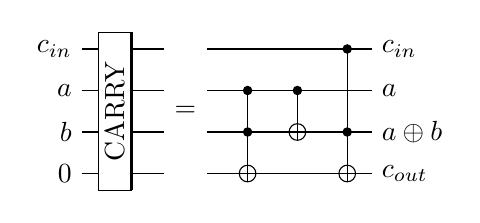
\begin{tikzpicture}[scale=1.000000,x=1pt,y=1pt]
\filldraw[color=white] (0.000000, -7.500000) rectangle (105.000000, 52.500000);
% Drawing wires
% Line 1: 0 W c_{in} c_{in}
\draw[color=black] (0.000000,45.000000) -- (105.000000,45.000000);
\draw[color=black] (0.000000,45.000000) node[left] {$c_{in}$};
% Line 2: 1 W a a
\draw[color=black] (0.000000,30.000000) -- (105.000000,30.000000);
\draw[color=black] (0.000000,30.000000) node[left] {$a$};
% Line 3: 2 W b a\oplus{b}
\draw[color=black] (0.000000,15.000000) -- (105.000000,15.000000);
\draw[color=black] (0.000000,15.000000) node[left] {$b$};
% Line 4: 3 W 0 c_{out}
\draw[color=black] (0.000000,0.000000) -- (105.000000,0.000000);
\draw[color=black] (0.000000,0.000000) node[left] {$0$};
% Done with wires; drawing gates
% Line 6: 0 1 2 3  G| \rotatebox{90}{CARRY}
\draw (12.000000,45.000000) -- (12.000000,0.000000);
\begin{scope}
\draw[fill=white] (12.000000, 22.500000) +(-45.000000:8.485281pt and 40.305087pt) -- +(45.000000:8.485281pt and 40.305087pt) -- +(135.000000:8.485281pt and 40.305087pt) -- +(225.000000:8.485281pt and 40.305087pt) -- cycle;
\draw[very thick,solid] (12.000000, 22.500000) +(-45.000000:8.485281pt and 40.305087pt) -- +(45.000000:8.485281pt and 40.305087pt);
\clip (12.000000, 22.500000) +(-45.000000:8.485281pt and 40.305087pt) -- +(45.000000:8.485281pt and 40.305087pt) -- +(135.000000:8.485281pt and 40.305087pt) -- +(225.000000:8.485281pt and 40.305087pt) -- cycle;
\draw (12.000000, 22.500000) node {\rotatebox{90}{CARRY}};
\end{scope}
% Line 7: =
\draw[fill=white,color=white] (30.000000, -6.000000) rectangle (45.000000, 51.000000);
\draw (37.500000, 22.500000) node {$=$};
% Line 9: +3 1 2
\draw (60.000000,30.000000) -- (60.000000,0.000000);
\begin{scope}
\draw[fill=white] (60.000000, 0.000000) circle(3.000000pt);
\clip (60.000000, 0.000000) circle(3.000000pt);
\draw (57.000000, 0.000000) -- (63.000000, 0.000000);
\draw (60.000000, -3.000000) -- (60.000000, 3.000000);
\end{scope}
\filldraw (60.000000, 30.000000) circle(1.500000pt);
\filldraw (60.000000, 15.000000) circle(1.500000pt);
% Line 10: +2 1
\draw (78.000000,30.000000) -- (78.000000,15.000000);
\begin{scope}
\draw[fill=white] (78.000000, 15.000000) circle(3.000000pt);
\clip (78.000000, 15.000000) circle(3.000000pt);
\draw (75.000000, 15.000000) -- (81.000000, 15.000000);
\draw (78.000000, 12.000000) -- (78.000000, 18.000000);
\end{scope}
\filldraw (78.000000, 30.000000) circle(1.500000pt);
% Line 11: +3 0 2
\draw (96.000000,45.000000) -- (96.000000,0.000000);
\begin{scope}
\draw[fill=white] (96.000000, 0.000000) circle(3.000000pt);
\clip (96.000000, 0.000000) circle(3.000000pt);
\draw (93.000000, 0.000000) -- (99.000000, 0.000000);
\draw (96.000000, -3.000000) -- (96.000000, 3.000000);
\end{scope}
\filldraw (96.000000, 45.000000) circle(1.500000pt);
\filldraw (96.000000, 15.000000) circle(1.500000pt);
% Done with gates; drawing ending labels
\draw[color=black] (105.000000,45.000000) node[right] {$c_{in}$};
\draw[color=black] (105.000000,30.000000) node[right] {$a$};
\draw[color=black] (105.000000,15.000000) node[right] {$a\oplus{b}$};
\draw[color=black] (105.000000,0.000000) node[right] {$c_{out}$};
% Done with ending labels; drawing cut lines and comments
% Done with comments
\end{tikzpicture}

\end{figure}

\SaveVerb{name}|Adder_VBE_Sum|
\begin{figure}[ht]
\caption{\protect\UseVerb{name}}
%! \usepackage{hyperref}
\hypertarget{VBE-sum}{}
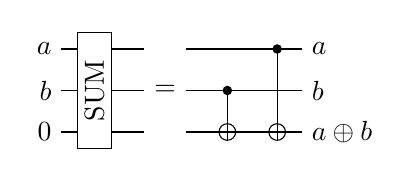
\begin{tikzpicture}[scale=1.000000,x=1pt,y=1pt]
\filldraw[color=white] (0.000000, -7.500000) rectangle (87.000000, 37.500000);
% Drawing wires
% Line 2: 1 W a a
\draw[color=black] (0.000000,30.000000) -- (87.000000,30.000000);
\draw[color=black] (0.000000,30.000000) node[left] {$a$};
% Line 3: 2 W b b
\draw[color=black] (0.000000,15.000000) -- (87.000000,15.000000);
\draw[color=black] (0.000000,15.000000) node[left] {$b$};
% Line 4: 3 W 0 a\oplus{b}
\draw[color=black] (0.000000,0.000000) -- (87.000000,0.000000);
\draw[color=black] (0.000000,0.000000) node[left] {$0$};
% Done with wires; drawing gates
% Line 6: 1 2 3  G \rotatebox{90}{SUM}
\draw (12.000000,30.000000) -- (12.000000,0.000000);
\begin{scope}
\draw[fill=white] (12.000000, 15.000000) +(-45.000000:8.485281pt and 29.698485pt) -- +(45.000000:8.485281pt and 29.698485pt) -- +(135.000000:8.485281pt and 29.698485pt) -- +(225.000000:8.485281pt and 29.698485pt) -- cycle;
\clip (12.000000, 15.000000) +(-45.000000:8.485281pt and 29.698485pt) -- +(45.000000:8.485281pt and 29.698485pt) -- +(135.000000:8.485281pt and 29.698485pt) -- +(225.000000:8.485281pt and 29.698485pt) -- cycle;
\draw (12.000000, 15.000000) node {\rotatebox{90}{SUM}};
\end{scope}
% Line 7: =
\draw[fill=white,color=white] (30.000000, -6.000000) rectangle (45.000000, 36.000000);
\draw (37.500000, 15.000000) node {$=$};
% Line 8: +3 2
\draw (60.000000,15.000000) -- (60.000000,0.000000);
\begin{scope}
\draw[fill=white] (60.000000, 0.000000) circle(3.000000pt);
\clip (60.000000, 0.000000) circle(3.000000pt);
\draw (57.000000, 0.000000) -- (63.000000, 0.000000);
\draw (60.000000, -3.000000) -- (60.000000, 3.000000);
\end{scope}
\filldraw (60.000000, 15.000000) circle(1.500000pt);
% Line 9: +3 1
\draw (78.000000,30.000000) -- (78.000000,0.000000);
\begin{scope}
\draw[fill=white] (78.000000, 0.000000) circle(3.000000pt);
\clip (78.000000, 0.000000) circle(3.000000pt);
\draw (75.000000, 0.000000) -- (81.000000, 0.000000);
\draw (78.000000, -3.000000) -- (78.000000, 3.000000);
\end{scope}
\filldraw (78.000000, 30.000000) circle(1.500000pt);
% Done with gates; drawing ending labels
\draw[color=black] (87.000000,30.000000) node[right] {$a$};
\draw[color=black] (87.000000,15.000000) node[right] {$b$};
\draw[color=black] (87.000000,0.000000) node[right] {$a\oplus{b}$};
% Done with ending labels; drawing cut lines and comments
% Done with comments
\end{tikzpicture}

\end{figure}

\SaveVerb{name}|AutoTest|
\begin{figure}[ht]
\caption{\protect\UseVerb{name}}
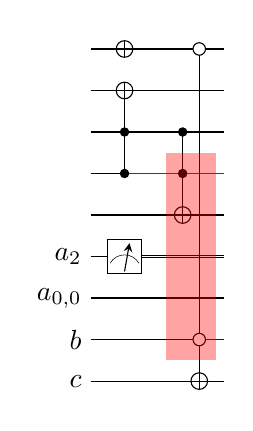
\begin{tikzpicture}[scale=1.000000,x=1pt,y=1pt]
\filldraw[color=white] (0.000000, -7.500000) rectangle (48.000000, 127.500000);
% Drawing wires
% Line 3: a W
\draw[color=black] (0.000000,120.000000) -- (48.000000,120.000000);
% Line 2: +0 1 2:color=purple
\draw[color=black] (0.000000,105.000000) -- (48.000000,105.000000);
% Line 2: +0 1 2:color=purple
\draw[color=black] (0.000000,90.000000) -- (48.000000,90.000000);
% Line 2: +0 1 2:color=purple
\draw[color=black] (0.000000,75.000000) -- (12.000000,75.000000);
\draw[color=purple] (12.000000,75.000000) -- (48.000000,75.000000);
% Line 5: 1 2 +3
\draw[color=black] (0.000000,60.000000) -- (48.000000,60.000000);
% Line 8: a2 M
\draw[color=black] (0.000000,45.000000) -- (12.000000,45.000000);
\draw[color=black] (12.000000,44.500000) -- (48.000000,44.500000);
\draw[color=black] (12.000000,45.500000) -- (48.000000,45.500000);
\draw[color=black] (0.000000,45.000000) node[left] {$a_{2}$};
% Line 9: a0,0 TOUCH
\draw[color=black] (0.000000,30.000000) -- (48.000000,30.000000);
\draw[color=black] (0.000000,30.000000) node[left] {$a_{0,0}$};
% Line 6: +c -a -b:color=blue
\draw[color=black] (0.000000,15.000000) -- (39.000000,15.000000);
\draw[color=blue] (39.000000,15.000000) -- (48.000000,15.000000);
\draw[color=black] (0.000000,15.000000) node[left] {$b$};
% Line 6: +c -a -b:color=blue
\draw[color=black] (0.000000,0.000000) -- (48.000000,0.000000);
\draw[color=black] (0.000000,0.000000) node[left] {$c$};
% Done with wires; drawing gates
% Line 2: +0 1 2:color=purple
\draw (12.000000,105.000000) -- (12.000000,75.000000);
\begin{scope}
\draw[fill=white] (12.000000, 105.000000) circle(3.000000pt);
\clip (12.000000, 105.000000) circle(3.000000pt);
\draw (9.000000, 105.000000) -- (15.000000, 105.000000);
\draw (12.000000, 102.000000) -- (12.000000, 108.000000);
\end{scope}
\filldraw (12.000000, 90.000000) circle(1.500000pt);
\filldraw (12.000000, 75.000000) circle(1.500000pt);
% Line 4: +a
\begin{scope}
\draw[fill=white] (12.000000, 120.000000) circle(3.000000pt);
\clip (12.000000, 120.000000) circle(3.000000pt);
\draw (9.000000, 120.000000) -- (15.000000, 120.000000);
\draw (12.000000, 117.000000) -- (12.000000, 123.000000);
\end{scope}
% Line 8: a2 M
\draw[fill=white] (6.000000, 39.000000) rectangle (18.000000, 51.000000);
\draw[very thin] (12.000000, 45.600000) arc (90:150:6.000000pt);
\draw[very thin] (12.000000, 45.600000) arc (90:30:6.000000pt);
\draw[->,>=stealth] (12.000000, 39.600000) -- +(80:10.392305pt);
% Line 9: a0,0 TOUCH
% Line 5: 1 2 +3
\draw (33.000000,90.000000) -- (33.000000,60.000000);
\filldraw (33.000000, 90.000000) circle(1.500000pt);
\filldraw (33.000000, 75.000000) circle(1.500000pt);
\begin{scope}
\draw[fill=white] (33.000000, 60.000000) circle(3.000000pt);
\clip (33.000000, 60.000000) circle(3.000000pt);
\draw (30.000000, 60.000000) -- (36.000000, 60.000000);
\draw (33.000000, 57.000000) -- (33.000000, 63.000000);
\end{scope}
% Line 6: +c -a -b:color=blue
\draw (39.000000,120.000000) -- (39.000000,0.000000);
\begin{scope}
\draw[fill=white] (39.000000, 0.000000) circle(3.000000pt);
\clip (39.000000, 0.000000) circle(3.000000pt);
\draw (36.000000, 0.000000) -- (42.000000, 0.000000);
\draw (39.000000, -3.000000) -- (39.000000, 3.000000);
\end{scope}
\draw[fill=white] (39.000000, 120.000000) circle(2.250000pt);
\draw[fill=white] (39.000000, 15.000000) circle(2.250000pt);
% Done with gates; drawing ending labels
% Done with ending labels; drawing cut lines and comments
% Line 7: 2 b @ 1 fill=red
\draw[draw opacity=0.000000,fill opacity=0.200000,fill=red] (27.000000,82.500000) rectangle (45.000000,7.500000);
\draw[draw opacity=0.000000,fill opacity=0.200000,fill=red] (27.000000,82.500000) rectangle (45.000000,7.500000);
% Done with comments
\end{tikzpicture}

\end{figure}

\SaveVerb{name}|BasicTeleportation|
\begin{figure}[ht]
\caption{\protect\UseVerb{name}}
%! \usetikzlibrary{decorations.pathreplacing,decorations.pathmorphing}
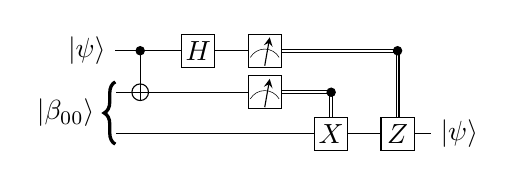
\begin{tikzpicture}[scale=1.000000,x=1pt,y=1pt]
\filldraw[color=white] (0.000000, -7.500000) rectangle (114.000000, 37.500000);
% Drawing wires
% Line 1: a W |\psi\rangle
\draw[color=black] (0.000000,30.000000) -- (54.000000,30.000000);
\draw[color=black] (54.000000,29.500000) -- (102.000000,29.500000);
\draw[color=black] (54.000000,30.500000) -- (102.000000,30.500000);
\draw[color=black] (0.000000,30.000000) node[left] {$|\psi\rangle$};
% Line 2: b c W |\beta_{00}\rangle<
\draw[color=black] (0.000000,15.000000) -- (54.000000,15.000000);
\draw[color=black] (54.000000,14.500000) -- (78.000000,14.500000);
\draw[color=black] (54.000000,15.500000) -- (78.000000,15.500000);
%   Deferring wire label at (0.000000,15.000000)
% Line 2: b c W |\beta_{00}\rangle<
\draw[color=black] (0.000000,0.000000) -- (114.000000,0.000000);
\filldraw[color=white,fill=white] (0.000000,-3.750000) rectangle (-4.000000,18.750000);
\draw[decorate,decoration={brace,amplitude = 4.000000pt},very thick] (0.000000,-3.750000) -- (0.000000,18.750000);
\draw[color=black] (-4.000000,7.500000) node[left] {$|\beta_{00}\rangle$};
% Done with wires; drawing gates
% Line 4: a +b
\draw (9.000000,30.000000) -- (9.000000,15.000000);
\filldraw (9.000000, 30.000000) circle(1.500000pt);
\begin{scope}
\draw[fill=white] (9.000000, 15.000000) circle(3.000000pt);
\clip (9.000000, 15.000000) circle(3.000000pt);
\draw (6.000000, 15.000000) -- (12.000000, 15.000000);
\draw (9.000000, 12.000000) -- (9.000000, 18.000000);
\end{scope}
% Line 5: a H
\begin{scope}
\draw[fill=white] (30.000000, 30.000000) +(-45.000000:8.485281pt and 8.485281pt) -- +(45.000000:8.485281pt and 8.485281pt) -- +(135.000000:8.485281pt and 8.485281pt) -- +(225.000000:8.485281pt and 8.485281pt) -- cycle;
\clip (30.000000, 30.000000) +(-45.000000:8.485281pt and 8.485281pt) -- +(45.000000:8.485281pt and 8.485281pt) -- +(135.000000:8.485281pt and 8.485281pt) -- +(225.000000:8.485281pt and 8.485281pt) -- cycle;
\draw (30.000000, 30.000000) node {$H$};
\end{scope}
% Line 6: a b M
\draw[fill=white] (48.000000, 24.000000) rectangle (60.000000, 36.000000);
\draw[very thin] (54.000000, 30.600000) arc (90:150:6.000000pt);
\draw[very thin] (54.000000, 30.600000) arc (90:30:6.000000pt);
\draw[->,>=stealth] (54.000000, 24.600000) -- +(80:10.392305pt);
\draw[fill=white] (48.000000, 9.000000) rectangle (60.000000, 21.000000);
\draw[very thin] (54.000000, 15.600000) arc (90:150:6.000000pt);
\draw[very thin] (54.000000, 15.600000) arc (90:30:6.000000pt);
\draw[->,>=stealth] (54.000000, 9.600000) -- +(80:10.392305pt);
% Line 7: c X b:owire
\draw (77.500000,15.000000) -- (77.500000,0.000000);
\draw (78.500000,15.000000) -- (78.500000,0.000000);
\begin{scope}
\draw[fill=white] (78.000000, -0.000000) +(-45.000000:8.485281pt and 8.485281pt) -- +(45.000000:8.485281pt and 8.485281pt) -- +(135.000000:8.485281pt and 8.485281pt) -- +(225.000000:8.485281pt and 8.485281pt) -- cycle;
\clip (78.000000, -0.000000) +(-45.000000:8.485281pt and 8.485281pt) -- +(45.000000:8.485281pt and 8.485281pt) -- +(135.000000:8.485281pt and 8.485281pt) -- +(225.000000:8.485281pt and 8.485281pt) -- cycle;
\draw (78.000000, -0.000000) node {$X$};
\end{scope}
\filldraw (78.000000, 15.000000) circle(1.500000pt);
% Line 8: c Z a:owire
\draw (101.500000,30.000000) -- (101.500000,0.000000);
\draw (102.500000,30.000000) -- (102.500000,0.000000);
\begin{scope}
\draw[fill=white] (102.000000, -0.000000) +(-45.000000:8.485281pt and 8.485281pt) -- +(45.000000:8.485281pt and 8.485281pt) -- +(135.000000:8.485281pt and 8.485281pt) -- +(225.000000:8.485281pt and 8.485281pt) -- cycle;
\clip (102.000000, -0.000000) +(-45.000000:8.485281pt and 8.485281pt) -- +(45.000000:8.485281pt and 8.485281pt) -- +(135.000000:8.485281pt and 8.485281pt) -- +(225.000000:8.485281pt and 8.485281pt) -- cycle;
\draw (102.000000, -0.000000) node {$Z$};
\end{scope}
\filldraw (102.000000, 30.000000) circle(1.500000pt);
% Done with gates; drawing ending labels
\draw[color=black] (114.000000,0.000000) node[right] {$|\psi\rangle$};
% Done with ending labels; drawing cut lines and comments
% Done with comments
\end{tikzpicture}

\end{figure}
\clearpage

\SaveVerb{name}|CoherentSuperDenseCoding|
\begin{figure}[ht]
\caption{\protect\UseVerb{name}}
\providecommand{\ket}[1]{\left|#1\right\rangle}
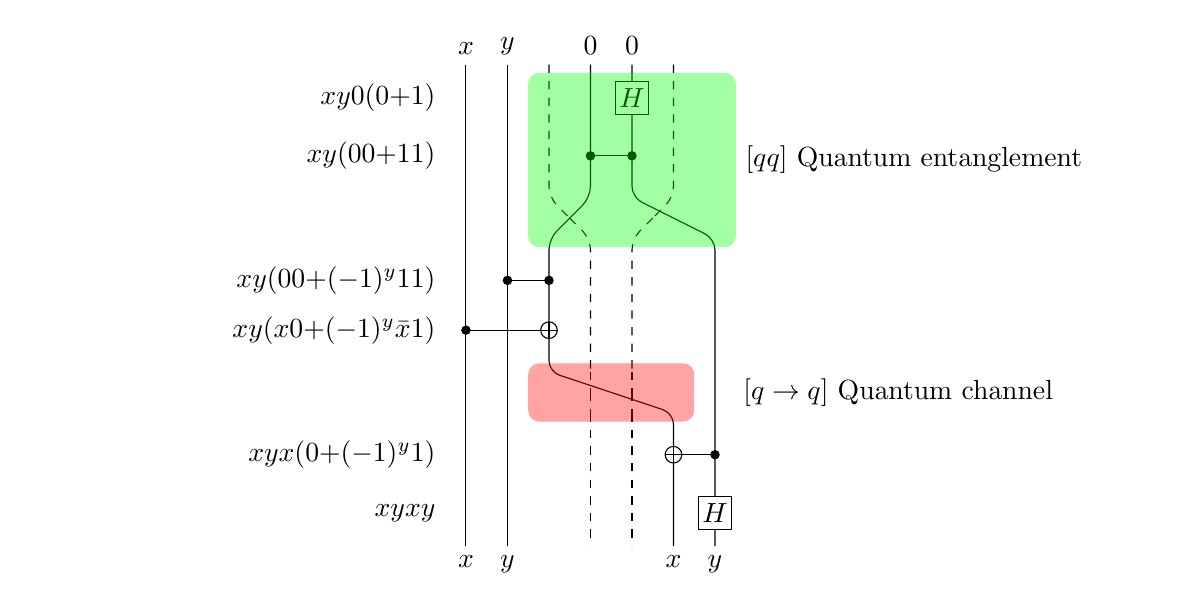
\begin{tikzpicture}[scale=1.000000,x=1pt,y=1pt]
\filldraw[color=white] (7.500000, 0.000000) rectangle (-97.500000, -174.000000);
% Drawing wires
% Line 2: a0 W \ket{x} \ket{x}
\draw[color=black] (-90.000000,0.000000) -- (-90.000000,-174.000000);
\draw[color=black] (-90.000000,0.000000) node[above] {$\ket{x}$};
% Line 3: a1 W \ket{y} \ket{y}
\draw[color=black] (-75.000000,0.000000) -- (-75.000000,-174.000000);
\draw[color=black] (-75.000000,0.000000) node[above] {$\ket{y}$};
% Line 4: x1 W style=dashed
\draw[color=black,dashed,rounded corners=4.000000pt] (-60.000000,0.000000) -- (-60.000000,-48.000000) -- (-52.500000,-55.500000);
\draw[color=black,dashed,rounded corners=4.000000pt] (-52.500000,-55.500000) -- (-45.000000,-63.000000) -- (-45.000000,-111.000000);
\draw[color=black,dashed] (-45.000000,-111.000000) -- (-45.000000,-118.500000);
\draw[color=black,dashed] (-45.000000,-118.500000) -- (-45.000000,-126.000000);
\draw[color=black,dashed] (-45.000000,-126.000000) -- (-45.000000,-174.000000);
% Line 6: b0 W \ket{0} \ket{x}
\draw[color=black,rounded corners=4.000000pt] (-45.000000,0.000000) -- (-45.000000,-48.000000) -- (-52.500000,-55.500000);
\draw[color=black,rounded corners=4.000000pt] (-52.500000,-55.500000) -- (-60.000000,-63.000000) -- (-60.000000,-111.000000) -- (-37.500000,-118.500000);
\draw[color=black,rounded corners=4.000000pt] (-37.500000,-118.500000) -- (-15.000000,-126.000000) -- (-15.000000,-174.000000);
\draw[color=black] (-45.000000,0.000000) node[above] {$\ket{0}$};
% Line 7: b1 W \ket{0} \ket{y}
\draw[color=black,rounded corners=4.000000pt] (-30.000000,0.000000) -- (-30.000000,-48.000000) -- (-15.000000,-55.500000);
\draw[color=black,rounded corners=4.000000pt] (-15.000000,-55.500000) -- (-0.000000,-63.000000) -- (-0.000000,-174.000000);
\draw[color=black] (-30.000000,0.000000) node[above] {$\ket{0}$};
% Line 8: x2 W style=dashed
\draw[color=black,dashed,rounded corners=4.000000pt] (-15.000000,0.000000) -- (-15.000000,-48.000000) -- (-22.500000,-55.500000);
\draw[color=black,dashed,rounded corners=4.000000pt] (-22.500000,-55.500000) -- (-30.000000,-63.000000) -- (-30.000000,-111.000000);
\draw[color=black,dashed] (-30.000000,-111.000000) -- (-30.000000,-118.500000);
\draw[color=black,dashed] (-30.000000,-118.500000) -- (-30.000000,-126.000000);
\draw[color=black,dashed] (-30.000000,-126.000000) -- (-30.000000,-174.000000);
% Line 9: blank W type=o
% Done with wires; drawing gates
% Line 12: b1 H    % $\ket{xy}\ket{0}(\ket{0}{+}\ket{1})$
\draw (-97.500000, -12.000000) node[text width=144pt,left,text ragged left] {$\ket{xy}\ket{0}(\ket{0}{+}\ket{1})$};
\begin{scope}
\draw[fill=white] (-30.000000, -12.000000) +(-45.000000:8.485281pt and 8.485281pt) -- +(45.000000:8.485281pt and 8.485281pt) -- +(135.000000:8.485281pt and 8.485281pt) -- +(225.000000:8.485281pt and 8.485281pt) -- cycle;
\clip (-30.000000, -12.000000) +(-45.000000:8.485281pt and 8.485281pt) -- +(45.000000:8.485281pt and 8.485281pt) -- +(135.000000:8.485281pt and 8.485281pt) -- +(225.000000:8.485281pt and 8.485281pt) -- cycle;
\draw (-30.000000, -12.000000) node {$H$};
\end{scope}
% Line 13: b0 b1   % $\ket{xy}(\ket{00}{+}\ket{11})$
\draw (-97.500000, -33.000000) node[text width=144pt,left,text ragged left] {$\ket{xy}(\ket{00}{+}\ket{11})$};
\draw (-45.000000,-33.000000) -- (-30.000000,-33.000000);
\filldraw (-45.000000, -33.000000) circle(1.500000pt);
\filldraw (-30.000000, -33.000000) circle(1.500000pt);
% Line 14: b0 x1 x2 blank b1 PERMUTE
% Line 15: a1 b0 % $\ket{xy}(\ket{00}{+}(-1)^{y}\ket{11})$
\draw (-97.500000, -78.000000) node[text width=144pt,left,text ragged left] {$\ket{xy}(\ket{00}{+}(-1)^{y}\ket{11})$};
\draw (-75.000000,-78.000000) -- (-60.000000,-78.000000);
\filldraw (-75.000000, -78.000000) circle(1.500000pt);
\filldraw (-60.000000, -78.000000) circle(1.500000pt);
% Line 16: +b0 a0 % $\ket{xy}(\ket{x 0}{+}(-1)^{y}\ket{\bar{x} 1})$
\draw (-97.500000, -96.000000) node[text width=144pt,left,text ragged left] {$\ket{xy}(\ket{x 0}{+}(-1)^{y}\ket{\bar{x} 1})$};
\draw (-90.000000,-96.000000) -- (-60.000000,-96.000000);
\begin{scope}
\draw[fill=white] (-60.000000, -96.000000) circle(3.000000pt);
\clip (-60.000000, -96.000000) circle(3.000000pt);
\draw (-63.000000, -96.000000) -- (-57.000000, -96.000000);
\draw (-60.000000, -99.000000) -- (-60.000000, -93.000000);
\end{scope}
\filldraw (-90.000000, -96.000000) circle(1.500000pt);
% Line 17: blank b0 PERMUTE
% Line 18: +b0 b1   % $\ket{xy}\ket{x}(\ket{0}{+}(-1)^{y}\ket{1})$
\draw (-97.500000, -141.000000) node[text width=144pt,left,text ragged left] {$\ket{xy}\ket{x}(\ket{0}{+}(-1)^{y}\ket{1})$};
\draw (-15.000000,-141.000000) -- (-0.000000,-141.000000);
\begin{scope}
\draw[fill=white] (-15.000000, -141.000000) circle(3.000000pt);
\clip (-15.000000, -141.000000) circle(3.000000pt);
\draw (-18.000000, -141.000000) -- (-12.000000, -141.000000);
\draw (-15.000000, -144.000000) -- (-15.000000, -138.000000);
\end{scope}
\filldraw (-0.000000, -141.000000) circle(1.500000pt);
% Line 19: b1 H    % $\ket{xy}\ket{x y}$
\draw (-97.500000, -162.000000) node[text width=144pt,left,text ragged left] {$\ket{xy}\ket{x y}$};
\begin{scope}
\draw[fill=white] (0.000000, -162.000000) +(-45.000000:8.485281pt and 8.485281pt) -- +(45.000000:8.485281pt and 8.485281pt) -- +(135.000000:8.485281pt and 8.485281pt) -- +(225.000000:8.485281pt and 8.485281pt) -- cycle;
\clip (0.000000, -162.000000) +(-45.000000:8.485281pt and 8.485281pt) -- +(45.000000:8.485281pt and 8.485281pt) -- +(135.000000:8.485281pt and 8.485281pt) -- +(225.000000:8.485281pt and 8.485281pt) -- cycle;
\draw (0.000000, -162.000000) node {$H$};
\end{scope}
% Done with gates; drawing ending labels
\draw[color=black] (-90.000000,-174.000000) node[below] {$\ket{x}$};
\draw[color=black] (-75.000000,-174.000000) node[below] {$\ket{y}$};
\draw[color=black] (-15.000000,-174.000000) node[below] {$\ket{x}$};
\draw[color=black] (-0.000000,-174.000000) node[below] {$\ket{y}$};
% Done with ending labels; drawing cut lines and comments
% Line 22: x1 b1 x2 blank @ 0 2 fill=green style=rounded_corners %% $[qq]$ Quantum entanglement
\draw[draw opacity=0.000000,fill opacity=0.200000,fill=green,rounded corners] (-67.500000,-3.000000) rectangle (7.500000,-66.000000);
\draw (7.500000, -34.500000) node[text width=144pt,right] {$[qq]$ Quantum entanglement};
\draw[draw opacity=0.000000,fill opacity=0.200000,fill=green,rounded corners] (-67.500000,-3.000000) rectangle (7.500000,-66.000000);
% Line 23: b0 x1 x2 blank @ 5 5 fill=red style=rounded_corners %% \hspace{.5cm}$[q\rightarrow q]$ Quantum channel
\draw[draw opacity=0.000000,fill opacity=0.200000,fill=red,rounded corners] (-67.500000,-108.000000) rectangle (-7.500000,-129.000000);
\draw (-7.500000, -118.500000) node[text width=144pt,right] {\hspace{.5cm}$[q\rightarrow q]$ Quantum channel};
\draw[draw opacity=0.000000,fill opacity=0.200000,fill=red,rounded corners] (-67.500000,-108.000000) rectangle (-7.500000,-129.000000);
% Done with comments
\end{tikzpicture}

\end{figure}

\SaveVerb{name}|ModAdder|
\begin{figure}[ht]
\caption{\protect\UseVerb{name}}
\providecommand{\ket}[1]{{\left\vert{#1}\right\rangle}}
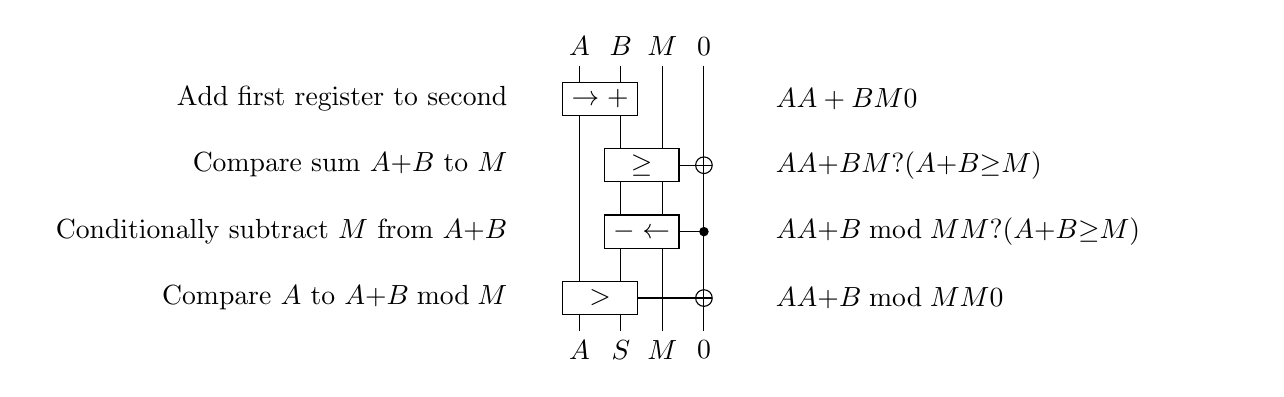
\begin{tikzpicture}[scale=1.000000,x=1pt,y=1pt]
\filldraw[color=white] (7.500000, 0.000000) rectangle (-82.500000, -96.000000);
% Drawing wires
% Line 5: aa W color=white
\draw[color=white] (-75.000000,0.000000) -- (-75.000000,-96.000000);
% Line 6: a W \ket{A} \ket{A}
\draw[color=black] (-60.000000,0.000000) -- (-60.000000,-96.000000);
\draw[color=black] (-60.000000,0.000000) node[above] {$\ket{A}$};
% Line 7: b W \ket{B} \ket{S}
\draw[color=black] (-45.000000,0.000000) -- (-45.000000,-96.000000);
\draw[color=black] (-45.000000,0.000000) node[above] {$\ket{B}$};
% Line 8: m W \ket{M} \ket{M}
\draw[color=black] (-30.000000,0.000000) -- (-30.000000,-96.000000);
\draw[color=black] (-30.000000,0.000000) node[above] {$\ket{M}$};
% Line 9: c W \ket{0} \ket{0}
\draw[color=black] (-15.000000,0.000000) -- (-15.000000,-96.000000);
\draw[color=black] (-15.000000,0.000000) node[above] {$\ket{0}$};
% Line 10: zz W color=white
\draw[color=white] (-0.000000,0.000000) -- (-0.000000,-96.000000);
% Done with wires; drawing gates
% Line 12: a b G $\rightarrow{}+$ % Add first register to second% $\ket{A}\ket{A+B}\ket{M}\ket{0}$
\draw (-82.500000, -12.000000) node[text width=170.0pt,left,text ragged left] {Add first register to second};
\draw (7.500000, -12.000000) node[text width=170.0pt,right] {$\ket{A}\ket{A+B}\ket{M}\ket{0}$};
\draw (-60.000000,-12.000000) -- (-45.000000,-12.000000);
\begin{scope}
\draw[fill=white] (-52.500000, -12.000000) +(-45.000000:19.091883pt and 8.485281pt) -- +(45.000000:19.091883pt and 8.485281pt) -- +(135.000000:19.091883pt and 8.485281pt) -- +(225.000000:19.091883pt and 8.485281pt) -- cycle;
\clip (-52.500000, -12.000000) +(-45.000000:19.091883pt and 8.485281pt) -- +(45.000000:19.091883pt and 8.485281pt) -- +(135.000000:19.091883pt and 8.485281pt) -- +(225.000000:19.091883pt and 8.485281pt) -- cycle;
\draw (-52.500000, -12.000000) node {$\rightarrow{}+$};
\end{scope}
% Line 13: b m G $\ge$ +c % Compare sum $A{+}B$ to $M$ % $\ket{A}\ket{A{+}B}\ket{M}\ket{?(A{+}B{\ge}M)}$
\draw (-82.500000, -36.000000) node[text width=170.0pt,left,text ragged left] {Compare sum $A{+}B$ to $M$};
\draw (7.500000, -36.000000) node[text width=170.0pt,right] {$\ket{A}\ket{A{+}B}\ket{M}\ket{?(A{+}B{\ge}M)}$};
\draw (-45.000000,-36.000000) -- (-15.000000,-36.000000);
\begin{scope}
\draw[fill=white] (-37.500000, -36.000000) +(-45.000000:19.091883pt and 8.485281pt) -- +(45.000000:19.091883pt and 8.485281pt) -- +(135.000000:19.091883pt and 8.485281pt) -- +(225.000000:19.091883pt and 8.485281pt) -- cycle;
\clip (-37.500000, -36.000000) +(-45.000000:19.091883pt and 8.485281pt) -- +(45.000000:19.091883pt and 8.485281pt) -- +(135.000000:19.091883pt and 8.485281pt) -- +(225.000000:19.091883pt and 8.485281pt) -- cycle;
\draw (-37.500000, -36.000000) node {$\ge$};
\end{scope}
\begin{scope}
\draw[fill=white] (-15.000000, -36.000000) circle(3.000000pt);
\clip (-15.000000, -36.000000) circle(3.000000pt);
\draw (-18.000000, -36.000000) -- (-12.000000, -36.000000);
\draw (-15.000000, -39.000000) -- (-15.000000, -33.000000);
\end{scope}
% Line 14: b m G $-\leftarrow$ c % Conditionally subtract $M$ from $A{+}B$% $\ket{A}\ket{A{+}B\bmod{}M}\ket{M}\ket{?(A{+}B{\ge}M)}$
\draw (-82.500000, -60.000000) node[text width=170.0pt,left,text ragged left] {Conditionally subtract $M$ from $A{+}B$};
\draw (7.500000, -60.000000) node[text width=170.0pt,right] {$\ket{A}\ket{A{+}B\bmod{}M}\ket{M}\ket{?(A{+}B{\ge}M)}$};
\draw (-45.000000,-60.000000) -- (-15.000000,-60.000000);
\begin{scope}
\draw[fill=white] (-37.500000, -60.000000) +(-45.000000:19.091883pt and 8.485281pt) -- +(45.000000:19.091883pt and 8.485281pt) -- +(135.000000:19.091883pt and 8.485281pt) -- +(225.000000:19.091883pt and 8.485281pt) -- cycle;
\clip (-37.500000, -60.000000) +(-45.000000:19.091883pt and 8.485281pt) -- +(45.000000:19.091883pt and 8.485281pt) -- +(135.000000:19.091883pt and 8.485281pt) -- +(225.000000:19.091883pt and 8.485281pt) -- cycle;
\draw (-37.500000, -60.000000) node {$-\leftarrow$};
\end{scope}
\filldraw (-15.000000, -60.000000) circle(1.500000pt);
% Line 15: a b G $>$ +c % Compare $A$ to $A{+}B\bmod M$ % $\ket{A}\ket{A{+}B\bmod{}M}\ket{M}\ket{0}$
\draw (-82.500000, -84.000000) node[text width=170.0pt,left,text ragged left] {Compare $A$ to $A{+}B\bmod M$};
\draw (7.500000, -84.000000) node[text width=170.0pt,right] {$\ket{A}\ket{A{+}B\bmod{}M}\ket{M}\ket{0}$};
\draw (-60.000000,-84.000000) -- (-15.000000,-84.000000);
\begin{scope}
\draw[fill=white] (-52.500000, -84.000000) +(-45.000000:19.091883pt and 8.485281pt) -- +(45.000000:19.091883pt and 8.485281pt) -- +(135.000000:19.091883pt and 8.485281pt) -- +(225.000000:19.091883pt and 8.485281pt) -- cycle;
\clip (-52.500000, -84.000000) +(-45.000000:19.091883pt and 8.485281pt) -- +(45.000000:19.091883pt and 8.485281pt) -- +(135.000000:19.091883pt and 8.485281pt) -- +(225.000000:19.091883pt and 8.485281pt) -- cycle;
\draw (-52.500000, -84.000000) node {$>$};
\end{scope}
\begin{scope}
\draw[fill=white] (-15.000000, -84.000000) circle(3.000000pt);
\clip (-15.000000, -84.000000) circle(3.000000pt);
\draw (-18.000000, -84.000000) -- (-12.000000, -84.000000);
\draw (-15.000000, -87.000000) -- (-15.000000, -81.000000);
\end{scope}
% Done with gates; drawing ending labels
\draw[color=black] (-60.000000,-96.000000) node[below] {$\ket{A}$};
\draw[color=black] (-45.000000,-96.000000) node[below] {$\ket{S}$};
\draw[color=black] (-30.000000,-96.000000) node[below] {$\ket{M}$};
\draw[color=black] (-15.000000,-96.000000) node[below] {$\ket{0}$};
% Done with ending labels; drawing cut lines and comments
% Done with comments
\end{tikzpicture}

\end{figure}

\SaveVerb{name}|ModExp|
\begin{figure}[ht]
\caption{\protect\UseVerb{name}}
\providecommand{\mynus}[1][.7]{\scalebox{#1}{-}}
\providecommand{\ket}[1]{{\left\vert{#1}\right\rangle}}
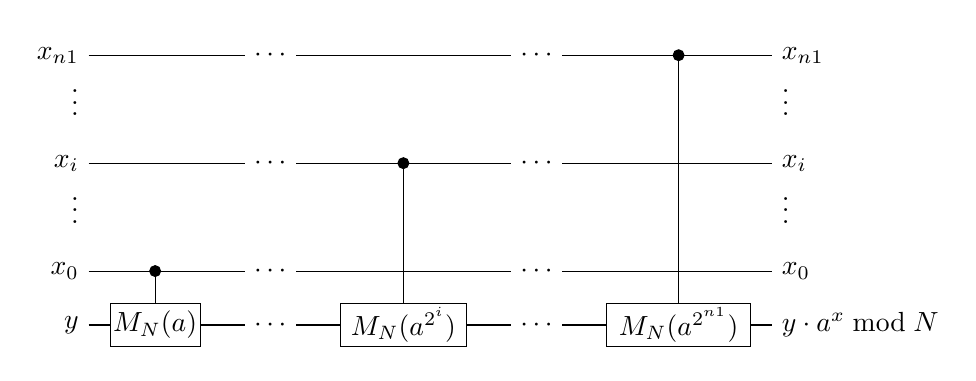
\begin{tikzpicture}[scale=1.300000,x=1pt,y=1pt]
\filldraw[color=white] (0.000000, -7.500000) rectangle (190.000000, 82.500000);
% Drawing wires
% Line 4: xn1 W \ket{x_{n\mynus1}} \ket{x_{n\mynus1}}
\draw[color=black] (0.000000,75.000000) -- (190.000000,75.000000);
\draw[color=black] (0.000000,75.000000) node[left] {$\ket{x_{n\mynus1}}$};
% Line 5: ...1 W
\draw[color=black] (0.000000,60.000000) node[anchor=mid east] {$\vdots$};
% Line 6: xi W \ket{x_i} \ket{x_i}
\draw[color=black] (0.000000,45.000000) -- (190.000000,45.000000);
\draw[color=black] (0.000000,45.000000) node[left] {$\ket{x_i}$};
% Line 7: ...2 W
\draw[color=black] (0.000000,30.000000) node[anchor=mid east] {$\vdots$};
% Line 9: x0 W \ket{x_0} \ket{x_0}
\draw[color=black] (0.000000,15.000000) -- (190.000000,15.000000);
\draw[color=black] (0.000000,15.000000) node[left] {$\ket{x_0}$};
% Line 10: y W \ket{y} \ket{y\cdot{}a^x\bmod{}N}
\draw[color=black] (0.000000,0.000000) -- (190.000000,0.000000);
\draw[color=black] (0.000000,0.000000) node[left] {$\ket{y}$};
% Done with wires; drawing gates
% Line 12: y G $M_N(a)$ x0 width=25
\draw (18.500000,15.000000) -- (18.500000,0.000000);
\begin{scope}
\draw[fill=white] (18.500000, -0.000000) +(-45.000000:17.677670pt and 8.485281pt) -- +(45.000000:17.677670pt and 8.485281pt) -- +(135.000000:17.677670pt and 8.485281pt) -- +(225.000000:17.677670pt and 8.485281pt) -- cycle;
\clip (18.500000, -0.000000) +(-45.000000:17.677670pt and 8.485281pt) -- +(45.000000:17.677670pt and 8.485281pt) -- +(135.000000:17.677670pt and 8.485281pt) -- +(225.000000:17.677670pt and 8.485281pt) -- cycle;
\draw (18.500000, -0.000000) node {$M_N(a)$};
\end{scope}
\filldraw (18.500000, 15.000000) circle(1.500000pt);
% Line 13: LABEL ...
\draw[color=black] (50.500000, 75.000000) node [fill=white] {$\cdots$};
\draw[color=black] (50.500000, 45.000000) node [fill=white] {$\cdots$};
\draw[color=black] (50.500000, 15.000000) node [fill=white] {$\cdots$};
\draw[color=black] (50.500000, 0.000000) node [fill=white] {$\cdots$};
% Line 14: y G $M_N(a^{2^i})$ xi width=35
\draw (87.500000,45.000000) -- (87.500000,0.000000);
\begin{scope}
\draw[fill=white] (87.500000, -0.000000) +(-45.000000:24.748737pt and 8.485281pt) -- +(45.000000:24.748737pt and 8.485281pt) -- +(135.000000:24.748737pt and 8.485281pt) -- +(225.000000:24.748737pt and 8.485281pt) -- cycle;
\clip (87.500000, -0.000000) +(-45.000000:24.748737pt and 8.485281pt) -- +(45.000000:24.748737pt and 8.485281pt) -- +(135.000000:24.748737pt and 8.485281pt) -- +(225.000000:24.748737pt and 8.485281pt) -- cycle;
\draw (87.500000, -0.000000) node {$M_N(a^{2^i})$};
\end{scope}
\filldraw (87.500000, 45.000000) circle(1.500000pt);
% Line 15: LABEL ...
\draw[color=black] (124.500000, 75.000000) node [fill=white] {$\cdots$};
\draw[color=black] (124.500000, 45.000000) node [fill=white] {$\cdots$};
\draw[color=black] (124.500000, 15.000000) node [fill=white] {$\cdots$};
\draw[color=black] (124.500000, 0.000000) node [fill=white] {$\cdots$};
% Line 16: y G $M_N(a^{2^{n\mynus1}})$ xn1 width=40
\draw (164.000000,75.000000) -- (164.000000,0.000000);
\begin{scope}
\draw[fill=white] (164.000000, -0.000000) +(-45.000000:28.284271pt and 8.485281pt) -- +(45.000000:28.284271pt and 8.485281pt) -- +(135.000000:28.284271pt and 8.485281pt) -- +(225.000000:28.284271pt and 8.485281pt) -- cycle;
\clip (164.000000, -0.000000) +(-45.000000:28.284271pt and 8.485281pt) -- +(45.000000:28.284271pt and 8.485281pt) -- +(135.000000:28.284271pt and 8.485281pt) -- +(225.000000:28.284271pt and 8.485281pt) -- cycle;
\draw (164.000000, -0.000000) node {$M_N(a^{2^{n\mynus1}})$};
\end{scope}
\filldraw (164.000000, 75.000000) circle(1.500000pt);
% Done with gates; drawing ending labels
\draw[color=black] (190.000000,75.000000) node[right] {$\ket{x_{n\mynus1}}$};
\draw[color=black] (190.000000,60.000000) node[anchor=mid west] {$\vdots$};
\draw[color=black] (190.000000,45.000000) node[right] {$\ket{x_i}$};
\draw[color=black] (190.000000,30.000000) node[anchor=mid west] {$\vdots$};
\draw[color=black] (190.000000,15.000000) node[right] {$\ket{x_0}$};
\draw[color=black] (190.000000,0.000000) node[right] {$\ket{y\cdot{}a^x\bmod{}N}$};
% Done with ending labels; drawing cut lines and comments
% Done with comments
\end{tikzpicture}

\end{figure}

\SaveVerb{name}|NestedLevels|
\begin{figure}[ht]
\caption{\protect\UseVerb{name}}
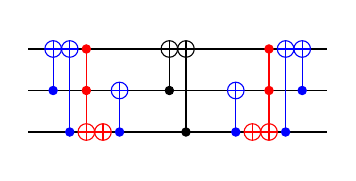
\begin{tikzpicture}[scale=1.000000,x=1pt,y=1pt]
\filldraw[color=white] (0.000000, -7.500000) rectangle (108.000000, 37.500000);
% Drawing wires
% Line 1: a W
\draw[color=black] (0.000000,30.000000) -- (108.000000,30.000000);
% Line 2: b W
\draw[color=black] (0.000000,15.000000) -- (108.000000,15.000000);
% Line 3: c W
\draw[color=black] (0.000000,0.000000) -- (108.000000,0.000000);
% Done with wires; drawing gates
% Line 6: +a b
\begin{scope}[color=blue]
\draw (9.000000,30.000000) -- (9.000000,15.000000);
\begin{scope}
\draw[fill=white] (9.000000, 30.000000) circle(3.000000pt);
\clip (9.000000, 30.000000) circle(3.000000pt);
\draw (6.000000, 30.000000) -- (12.000000, 30.000000);
\draw (9.000000, 27.000000) -- (9.000000, 33.000000);
\end{scope}
\filldraw (9.000000, 15.000000) circle(1.500000pt);
\draw (99.000000,30.000000) -- (99.000000,15.000000);
\begin{scope}
\draw[fill=white] (99.000000, 30.000000) circle(3.000000pt);
\clip (99.000000, 30.000000) circle(3.000000pt);
\draw (96.000000, 30.000000) -- (102.000000, 30.000000);
\draw (99.000000, 27.000000) -- (99.000000, 33.000000);
\end{scope}
\filldraw (99.000000, 15.000000) circle(1.500000pt);
\end{scope}
% Line 7: +a c
\begin{scope}[color=blue]
\draw (15.000000,30.000000) -- (15.000000,0.000000);
\begin{scope}
\draw[fill=white] (15.000000, 30.000000) circle(3.000000pt);
\clip (15.000000, 30.000000) circle(3.000000pt);
\draw (12.000000, 30.000000) -- (18.000000, 30.000000);
\draw (15.000000, 27.000000) -- (15.000000, 33.000000);
\end{scope}
\filldraw (15.000000, 0.000000) circle(1.500000pt);
\draw (93.000000,30.000000) -- (93.000000,0.000000);
\begin{scope}
\draw[fill=white] (93.000000, 30.000000) circle(3.000000pt);
\clip (93.000000, 30.000000) circle(3.000000pt);
\draw (90.000000, 30.000000) -- (96.000000, 30.000000);
\draw (93.000000, 27.000000) -- (93.000000, 33.000000);
\end{scope}
\filldraw (93.000000, 0.000000) circle(1.500000pt);
\end{scope}
% Line 9: +c b a
\begin{scope}[color=red]
\draw (21.000000,30.000000) -- (21.000000,0.000000);
\begin{scope}
\draw[fill=white] (21.000000, 0.000000) circle(3.000000pt);
\clip (21.000000, 0.000000) circle(3.000000pt);
\draw (18.000000, 0.000000) -- (24.000000, 0.000000);
\draw (21.000000, -3.000000) -- (21.000000, 3.000000);
\end{scope}
\filldraw (21.000000, 15.000000) circle(1.500000pt);
\filldraw (21.000000, 30.000000) circle(1.500000pt);
\draw (87.000000,30.000000) -- (87.000000,0.000000);
\begin{scope}
\draw[fill=white] (87.000000, 0.000000) circle(3.000000pt);
\clip (87.000000, 0.000000) circle(3.000000pt);
\draw (84.000000, 0.000000) -- (90.000000, 0.000000);
\draw (87.000000, -3.000000) -- (87.000000, 3.000000);
\end{scope}
\filldraw (87.000000, 15.000000) circle(1.500000pt);
\filldraw (87.000000, 30.000000) circle(1.500000pt);
\end{scope}
% Line 10: +c
\begin{scope}[color=red]
\begin{scope}
\draw[fill=white] (27.000000, 0.000000) circle(3.000000pt);
\clip (27.000000, 0.000000) circle(3.000000pt);
\draw (24.000000, 0.000000) -- (30.000000, 0.000000);
\draw (27.000000, -3.000000) -- (27.000000, 3.000000);
\end{scope}
\begin{scope}
\draw[fill=white] (81.000000, 0.000000) circle(3.000000pt);
\clip (81.000000, 0.000000) circle(3.000000pt);
\draw (78.000000, 0.000000) -- (84.000000, 0.000000);
\draw (81.000000, -3.000000) -- (81.000000, 3.000000);
\end{scope}
\end{scope}
% Line 12: +b c
\begin{scope}[color=blue]
\draw (33.000000,15.000000) -- (33.000000,0.000000);
\begin{scope}
\draw[fill=white] (33.000000, 15.000000) circle(3.000000pt);
\clip (33.000000, 15.000000) circle(3.000000pt);
\draw (30.000000, 15.000000) -- (36.000000, 15.000000);
\draw (33.000000, 12.000000) -- (33.000000, 18.000000);
\end{scope}
\filldraw (33.000000, 0.000000) circle(1.500000pt);
\draw (75.000000,15.000000) -- (75.000000,0.000000);
\begin{scope}
\draw[fill=white] (75.000000, 15.000000) circle(3.000000pt);
\clip (75.000000, 15.000000) circle(3.000000pt);
\draw (72.000000, 15.000000) -- (78.000000, 15.000000);
\draw (75.000000, 12.000000) -- (75.000000, 18.000000);
\end{scope}
\filldraw (75.000000, 0.000000) circle(1.500000pt);
\end{scope}
% Line 17: +a b
\draw (51.000000,30.000000) -- (51.000000,15.000000);
\begin{scope}
\draw[fill=white] (51.000000, 30.000000) circle(3.000000pt);
\clip (51.000000, 30.000000) circle(3.000000pt);
\draw (48.000000, 30.000000) -- (54.000000, 30.000000);
\draw (51.000000, 27.000000) -- (51.000000, 33.000000);
\end{scope}
\filldraw (51.000000, 15.000000) circle(1.500000pt);
% Line 18: +a c
\draw (57.000000,30.000000) -- (57.000000,0.000000);
\begin{scope}
\draw[fill=white] (57.000000, 30.000000) circle(3.000000pt);
\clip (57.000000, 30.000000) circle(3.000000pt);
\draw (54.000000, 30.000000) -- (60.000000, 30.000000);
\draw (57.000000, 27.000000) -- (57.000000, 33.000000);
\end{scope}
\filldraw (57.000000, 0.000000) circle(1.500000pt);
% Done with gates; drawing ending labels
% Done with ending labels; drawing cut lines and comments
% Done with comments
\end{tikzpicture}

\end{figure}

\SaveVerb{name}|PleaseTouch|
\begin{figure}[ht]
\caption{\protect\UseVerb{name}}
%! \definecolor{bg}{rgb}{1,1,1}
%! \usetikzlibrary{decorations.pathreplacing,decorations.pathmorphing}
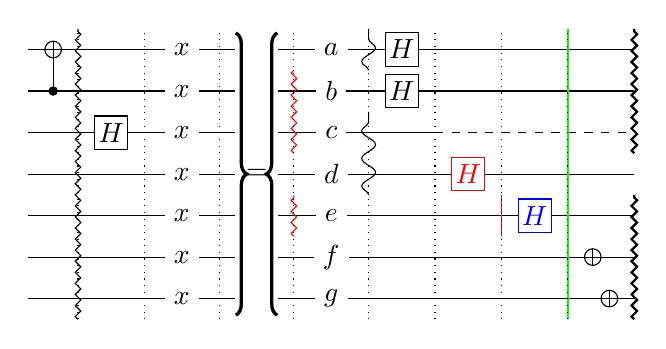
\begin{tikzpicture}[scale=1.000000,x=1pt,y=1pt]
\filldraw[color=bg] (0.000000, -7.500000) rectangle (219.000000, 97.500000);
% Drawing wires
% Line 2: 0 W
\draw[color=black] (0.000000,90.000000) -- (219.000000,90.000000);
% Line 3: 1 W
\draw[color=black] (0.000000,75.000000) -- (219.000000,75.000000);
% Line 4: 2 W
\draw[color=black] (0.000000,60.000000) -- (147.000000,60.000000);
\draw[color=black,dashed] (147.000000,60.000000) -- (219.000000,60.000000);
% Line 5: 3 W
\draw[color=black] (0.000000,45.000000) -- (219.000000,45.000000);
% Line 6: 4 W
\draw[color=black] (0.000000,30.000000) -- (219.000000,30.000000);
% Line 24: 5 W
\draw[color=black] (0.000000,15.000000) -- (219.000000,15.000000);
% Line 27: 6 W
\draw[color=black] (0.000000,0.000000) -- (219.000000,0.000000);
% Done with wires; drawing gates
% Line 9: +0 1
\draw (9.000000,90.000000) -- (9.000000,75.000000);
\begin{scope}
\draw[fill=bg] (9.000000, 90.000000) circle(3.000000pt);
\clip (9.000000, 90.000000) circle(3.000000pt);
\draw (6.000000, 90.000000) -- (12.000000, 90.000000);
\draw (9.000000, 87.000000) -- (9.000000, 93.000000);
\end{scope}
\filldraw (9.000000, 75.000000) circle(1.500000pt);
% Line 10: BARRIER
\draw[decorate,decoration={zigzag,amplitude=1pt,segment length=4}] (18.000000,-7.500000) -- (18.000000,97.500000);
% Line 11: 2 H
\begin{scope}
\draw[fill=bg] (30.000000, 60.000000) +(-45.000000:8.485281pt and 8.485281pt) -- +(45.000000:8.485281pt and 8.485281pt) -- +(135.000000:8.485281pt and 8.485281pt) -- +(225.000000:8.485281pt and 8.485281pt) -- cycle;
\clip (30.000000, 60.000000) +(-45.000000:8.485281pt and 8.485281pt) -- +(45.000000:8.485281pt and 8.485281pt) -- +(135.000000:8.485281pt and 8.485281pt) -- +(225.000000:8.485281pt and 8.485281pt) -- cycle;
\draw (30.000000, 60.000000) node {$H$};
\end{scope}
% Line 12: LABEL x
\draw[color=black] (55.500000, 90.000000) node [fill=bg] {$x$};
\draw[color=black] (55.500000, 75.000000) node [fill=bg] {$x$};
\draw[color=black] (55.500000, 60.000000) node [fill=bg] {$x$};
\draw[color=black] (55.500000, 45.000000) node [fill=bg] {$x$};
\draw[color=black] (55.500000, 30.000000) node [fill=bg] {$x$};
\draw[color=black] (55.500000, 15.000000) node [fill=bg] {$x$};
\draw[color=black] (55.500000, 0.000000) node [fill=bg] {$x$};
% Line 13: >=<
\draw[fill=bg,color=bg] (75.000000, -6.000000) rectangle (90.000000, 96.000000);
\draw (82.500000, 45.000000) node {$=$};
\draw[decorate,decoration={brace,mirror,amplitude = 4.000000pt},very thick] (75.000000,-6.000000) -- (75.000000,96.000000);
\draw[decorate,decoration={brace,amplitude = 4.000000pt},very thick] (90.000000,-6.000000) -- (90.000000,96.000000);
% Line 14: 1 2 4 BARRIER color=red
\begin{scope}[color=red]
\draw[decorate,decoration={zigzag,amplitude=1pt,segment length=4}] (96.000000,22.500000) -- (96.000000,37.500000);
\draw[decorate,decoration={zigzag,amplitude=1pt,segment length=4}] (96.000000,52.500000) -- (96.000000,82.500000);
\end{scope}
% Line 15: LABEL a b c d e f g
\draw[color=black] (109.500000, 90.000000) node [fill=bg] {$a$};
\draw[color=black] (109.500000, 75.000000) node [fill=bg] {$b$};
\draw[color=black] (109.500000, 60.000000) node [fill=bg] {$c$};
\draw[color=black] (109.500000, 45.000000) node [fill=bg] {$d$};
\draw[color=black] (109.500000, 30.000000) node [fill=bg] {$e$};
\draw[color=black] (109.500000, 15.000000) node [fill=bg] {$f$};
\draw[color=black] (109.500000, 0.000000) node [fill=bg] {$g$};
% Line 16: 0 2 3 TOUCH style=decorate,decoration=snake
\draw[decorate,decoration=snake] (123.000000,37.500000) -- (123.000000,67.500000);
\draw[decorate,decoration=snake] (123.000000,82.500000) -- (123.000000,97.500000);
% Line 17: 0 H
\begin{scope}
\draw[fill=bg] (135.000000, 90.000000) +(-45.000000:8.485281pt and 8.485281pt) -- +(45.000000:8.485281pt and 8.485281pt) -- +(135.000000:8.485281pt and 8.485281pt) -- +(225.000000:8.485281pt and 8.485281pt) -- cycle;
\clip (135.000000, 90.000000) +(-45.000000:8.485281pt and 8.485281pt) -- +(45.000000:8.485281pt and 8.485281pt) -- +(135.000000:8.485281pt and 8.485281pt) -- +(225.000000:8.485281pt and 8.485281pt) -- cycle;
\draw (135.000000, 90.000000) node {$H$};
\end{scope}
% Line 18: 1 H
\begin{scope}
\draw[fill=bg] (135.000000, 75.000000) +(-45.000000:8.485281pt and 8.485281pt) -- +(45.000000:8.485281pt and 8.485281pt) -- +(135.000000:8.485281pt and 8.485281pt) -- +(225.000000:8.485281pt and 8.485281pt) -- cycle;
\clip (135.000000, 75.000000) +(-45.000000:8.485281pt and 8.485281pt) -- +(45.000000:8.485281pt and 8.485281pt) -- +(135.000000:8.485281pt and 8.485281pt) -- +(225.000000:8.485281pt and 8.485281pt) -- cycle;
\draw (135.000000, 75.000000) node {$H$};
\end{scope}
% Line 19: 0 1 2:style=dashed 3 4 TOUCH
% Line 20: 3 H color=red
\begin{scope}[color=red]
\begin{scope}[color=red]
\begin{scope}
\draw[fill=bg] (159.000000, 45.000000) +(-45.000000:8.485281pt and 8.485281pt) -- +(45.000000:8.485281pt and 8.485281pt) -- +(135.000000:8.485281pt and 8.485281pt) -- +(225.000000:8.485281pt and 8.485281pt) -- cycle;
\clip (159.000000, 45.000000) +(-45.000000:8.485281pt and 8.485281pt) -- +(45.000000:8.485281pt and 8.485281pt) -- +(135.000000:8.485281pt and 8.485281pt) -- +(225.000000:8.485281pt and 8.485281pt) -- cycle;
\draw (159.000000, 45.000000) node {$H$};
\end{scope}
\end{scope}
\end{scope}
% Line 21: 4 TOUCH color=red
\begin{scope}[color=red]
\draw (171.000000,22.500000) -- (171.000000,37.500000);
\end{scope}
% Line 22: 4 H color=blue
\begin{scope}[color=blue]
\begin{scope}[color=blue]
\begin{scope}
\draw[fill=bg] (183.000000, 30.000000) +(-45.000000:8.485281pt and 8.485281pt) -- +(45.000000:8.485281pt and 8.485281pt) -- +(135.000000:8.485281pt and 8.485281pt) -- +(225.000000:8.485281pt and 8.485281pt) -- cycle;
\clip (183.000000, 30.000000) +(-45.000000:8.485281pt and 8.485281pt) -- +(45.000000:8.485281pt and 8.485281pt) -- +(135.000000:8.485281pt and 8.485281pt) -- +(225.000000:8.485281pt and 8.485281pt) -- cycle;
\draw (183.000000, 30.000000) node {$H$};
\end{scope}
\end{scope}
\end{scope}
% Line 23: TOUCH color=green style=thick
\begin{scope}[color=green]
\draw[thick] (195.000000,-7.500000) -- (195.000000,97.500000);
\end{scope}
% Line 25: 5 N
\begin{scope}
\draw[fill=bg] (204.000000, 15.000000) circle(3.000000pt);
\clip (204.000000, 15.000000) circle(3.000000pt);
\draw (201.000000, 15.000000) -- (207.000000, 15.000000);
\draw (204.000000, 12.000000) -- (204.000000, 18.000000);
\end{scope}
% Line 26: PHANTOM
% Line 28: +6
\begin{scope}
\draw[fill=bg] (210.000000, 0.000000) circle(3.000000pt);
\clip (210.000000, 0.000000) circle(3.000000pt);
\draw (207.000000, 0.000000) -- (213.000000, 0.000000);
\draw (210.000000, -3.000000) -- (210.000000, 3.000000);
\end{scope}
% Line 29: 0 1 2 4 5 6 BARRIER style=thick
\draw[decorate,decoration={zigzag,amplitude=1pt,segment length=4},thick] (219.000000,-7.500000) -- (219.000000,37.500000);
\draw[decorate,decoration={zigzag,amplitude=1pt,segment length=4},thick] (219.000000,52.500000) -- (219.000000,97.500000);
% Done with gates; drawing ending labels
% Done with ending labels; drawing cut lines and comments
\draw[dotted] (18.000000, -7.500000) -- (18.000000, 97.500000);
\draw[dotted] (42.000000, -7.500000) -- (42.000000, 97.500000);
\draw[dotted] (69.000000, -7.500000) -- (69.000000, 97.500000);
\draw[dotted] (96.000000, -7.500000) -- (96.000000, 97.500000);
\draw[dotted] (123.000000, -7.500000) -- (123.000000, 97.500000);
\draw[dotted] (147.000000, -7.500000) -- (147.000000, 97.500000);
\draw[dotted] (171.000000, -7.500000) -- (171.000000, 97.500000);
\draw[dotted] (195.000000, -7.500000) -- (195.000000, 97.500000);
% Done with comments
\end{tikzpicture}

\end{figure}

\SaveVerb{name}|QFT3v1|
\begin{figure}[ht]
\caption{\protect\UseVerb{name}}
\providecommand{\ket}[1]{\left|#1\right\rangle}
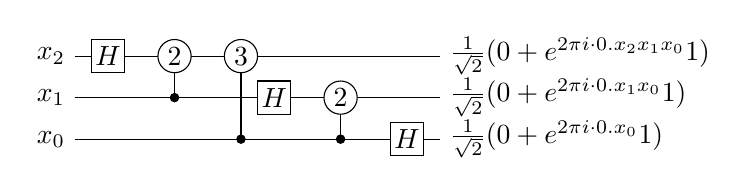
\begin{tikzpicture}[scale=1.000000,x=1pt,y=1pt]
\filldraw[color=white] (0.000000, -7.500000) rectangle (132.000000, 37.500000);
% Drawing wires
% Line 2: a2 W \ket{x_2} \frac{1}{\sqrt{2}}(\ket{0}+e^{2{\pi}i{\cdot0}.x_2x_1x_0}\ket{1})
\draw[color=black] (0.000000,30.000000) -- (132.000000,30.000000);
\draw[color=black] (0.000000,30.000000) node[left] {$\ket{x_2}$};
% Line 3: a1 W \ket{x_1} \frac{1}{\sqrt{2}}(\ket{0}+e^{2{\pi}i{\cdot0}.x_1x_0}\ket{1})
\draw[color=black] (0.000000,15.000000) -- (132.000000,15.000000);
\draw[color=black] (0.000000,15.000000) node[left] {$\ket{x_1}$};
% Line 4: a0 W \ket{x_0} \frac{1}{\sqrt{2}}(\ket{0}+e^{2{\pi}i{\cdot0}.x_0}\ket{1})
\draw[color=black] (0.000000,0.000000) -- (132.000000,0.000000);
\draw[color=black] (0.000000,0.000000) node[left] {$\ket{x_0}$};
% Done with wires; drawing gates
% Line 5: a2 H
\begin{scope}
\draw[fill=white] (12.000000, 30.000000) +(-45.000000:8.485281pt and 8.485281pt) -- +(45.000000:8.485281pt and 8.485281pt) -- +(135.000000:8.485281pt and 8.485281pt) -- +(225.000000:8.485281pt and 8.485281pt) -- cycle;
\clip (12.000000, 30.000000) +(-45.000000:8.485281pt and 8.485281pt) -- +(45.000000:8.485281pt and 8.485281pt) -- +(135.000000:8.485281pt and 8.485281pt) -- +(225.000000:8.485281pt and 8.485281pt) -- cycle;
\draw (12.000000, 30.000000) node {$H$};
\end{scope}
% Line 7: a2 P $2$ a1
\draw (36.000000,30.000000) -- (36.000000,15.000000);
\begin{scope}
\draw[fill=white] (36.000000, 30.000000) circle(6.000000pt);
\clip (36.000000, 30.000000) circle(6.000000pt);
\draw (36.000000, 30.000000) node {$2$};
\end{scope}
\filldraw (36.000000, 15.000000) circle(1.500000pt);
% Line 8: a2 P $3$ a0
\draw (60.000000,30.000000) -- (60.000000,0.000000);
\begin{scope}
\draw[fill=white] (60.000000, 30.000000) circle(6.000000pt);
\clip (60.000000, 30.000000) circle(6.000000pt);
\draw (60.000000, 30.000000) node {$3$};
\end{scope}
\filldraw (60.000000, 0.000000) circle(1.500000pt);
% Line 9: a1 H
\begin{scope}
\draw[fill=white] (72.000000, 15.000000) +(-45.000000:8.485281pt and 8.485281pt) -- +(45.000000:8.485281pt and 8.485281pt) -- +(135.000000:8.485281pt and 8.485281pt) -- +(225.000000:8.485281pt and 8.485281pt) -- cycle;
\clip (72.000000, 15.000000) +(-45.000000:8.485281pt and 8.485281pt) -- +(45.000000:8.485281pt and 8.485281pt) -- +(135.000000:8.485281pt and 8.485281pt) -- +(225.000000:8.485281pt and 8.485281pt) -- cycle;
\draw (72.000000, 15.000000) node {$H$};
\end{scope}
% Line 10: a1 P $2$ a0
\draw (96.000000,15.000000) -- (96.000000,0.000000);
\begin{scope}
\draw[fill=white] (96.000000, 15.000000) circle(6.000000pt);
\clip (96.000000, 15.000000) circle(6.000000pt);
\draw (96.000000, 15.000000) node {$2$};
\end{scope}
\filldraw (96.000000, 0.000000) circle(1.500000pt);
% Line 11: a0 H
\begin{scope}
\draw[fill=white] (120.000000, -0.000000) +(-45.000000:8.485281pt and 8.485281pt) -- +(45.000000:8.485281pt and 8.485281pt) -- +(135.000000:8.485281pt and 8.485281pt) -- +(225.000000:8.485281pt and 8.485281pt) -- cycle;
\clip (120.000000, -0.000000) +(-45.000000:8.485281pt and 8.485281pt) -- +(45.000000:8.485281pt and 8.485281pt) -- +(135.000000:8.485281pt and 8.485281pt) -- +(225.000000:8.485281pt and 8.485281pt) -- cycle;
\draw (120.000000, -0.000000) node {$H$};
\end{scope}
% Done with gates; drawing ending labels
\draw[color=black] (132.000000,30.000000) node[right] {$\frac{1}{\sqrt{2}}(\ket{0}+e^{2{\pi}i{\cdot0}.x_2x_1x_0}\ket{1})$};
\draw[color=black] (132.000000,15.000000) node[right] {$\frac{1}{\sqrt{2}}(\ket{0}+e^{2{\pi}i{\cdot0}.x_1x_0}\ket{1})$};
\draw[color=black] (132.000000,0.000000) node[right] {$\frac{1}{\sqrt{2}}(\ket{0}+e^{2{\pi}i{\cdot0}.x_0}\ket{1})$};
% Done with ending labels; drawing cut lines and comments
% Done with comments
\end{tikzpicture}

\end{figure}

\SaveVerb{name}|QFT3v2|
\begin{figure}[ht]
\caption{\protect\UseVerb{name}}
\providecommand{\ket}[1]{\left|#1\right\rangle}
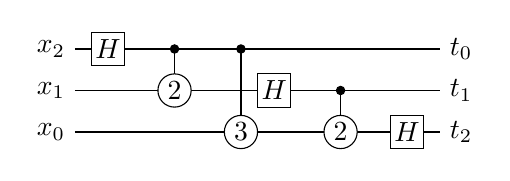
\begin{tikzpicture}[scale=1.000000,x=1pt,y=1pt]
\filldraw[color=white] (0.000000, -7.500000) rectangle (132.000000, 37.500000);
% Drawing wires
% Line 2: a2 W \ket{x_2} \ket{t_0}
\draw[color=black] (0.000000,30.000000) -- (132.000000,30.000000);
\draw[color=black] (0.000000,30.000000) node[left] {$\ket{x_2}$};
% Line 3: a1 W \ket{x_1} \ket{t_1}
\draw[color=black] (0.000000,15.000000) -- (132.000000,15.000000);
\draw[color=black] (0.000000,15.000000) node[left] {$\ket{x_1}$};
% Line 4: a0 W \ket{x_0} \ket{t_2}
\draw[color=black] (0.000000,0.000000) -- (132.000000,0.000000);
\draw[color=black] (0.000000,0.000000) node[left] {$\ket{x_0}$};
% Done with wires; drawing gates
% Line 5: a2 H
\begin{scope}
\draw[fill=white] (12.000000, 30.000000) +(-45.000000:8.485281pt and 8.485281pt) -- +(45.000000:8.485281pt and 8.485281pt) -- +(135.000000:8.485281pt and 8.485281pt) -- +(225.000000:8.485281pt and 8.485281pt) -- cycle;
\clip (12.000000, 30.000000) +(-45.000000:8.485281pt and 8.485281pt) -- +(45.000000:8.485281pt and 8.485281pt) -- +(135.000000:8.485281pt and 8.485281pt) -- +(225.000000:8.485281pt and 8.485281pt) -- cycle;
\draw (12.000000, 30.000000) node {$H$};
\end{scope}
% Line 7: a1 P $2$ a2
\draw (36.000000,30.000000) -- (36.000000,15.000000);
\begin{scope}
\draw[fill=white] (36.000000, 15.000000) circle(6.000000pt);
\clip (36.000000, 15.000000) circle(6.000000pt);
\draw (36.000000, 15.000000) node {$2$};
\end{scope}
\filldraw (36.000000, 30.000000) circle(1.500000pt);
% Line 8: a0 P $3$ a2
\draw (60.000000,30.000000) -- (60.000000,0.000000);
\begin{scope}
\draw[fill=white] (60.000000, 0.000000) circle(6.000000pt);
\clip (60.000000, 0.000000) circle(6.000000pt);
\draw (60.000000, 0.000000) node {$3$};
\end{scope}
\filldraw (60.000000, 30.000000) circle(1.500000pt);
% Line 9: a1 H
\begin{scope}
\draw[fill=white] (72.000000, 15.000000) +(-45.000000:8.485281pt and 8.485281pt) -- +(45.000000:8.485281pt and 8.485281pt) -- +(135.000000:8.485281pt and 8.485281pt) -- +(225.000000:8.485281pt and 8.485281pt) -- cycle;
\clip (72.000000, 15.000000) +(-45.000000:8.485281pt and 8.485281pt) -- +(45.000000:8.485281pt and 8.485281pt) -- +(135.000000:8.485281pt and 8.485281pt) -- +(225.000000:8.485281pt and 8.485281pt) -- cycle;
\draw (72.000000, 15.000000) node {$H$};
\end{scope}
% Line 10: a0 P $2$ a1
\draw (96.000000,15.000000) -- (96.000000,0.000000);
\begin{scope}
\draw[fill=white] (96.000000, 0.000000) circle(6.000000pt);
\clip (96.000000, 0.000000) circle(6.000000pt);
\draw (96.000000, 0.000000) node {$2$};
\end{scope}
\filldraw (96.000000, 15.000000) circle(1.500000pt);
% Line 11: a0 H
\begin{scope}
\draw[fill=white] (120.000000, -0.000000) +(-45.000000:8.485281pt and 8.485281pt) -- +(45.000000:8.485281pt and 8.485281pt) -- +(135.000000:8.485281pt and 8.485281pt) -- +(225.000000:8.485281pt and 8.485281pt) -- cycle;
\clip (120.000000, -0.000000) +(-45.000000:8.485281pt and 8.485281pt) -- +(45.000000:8.485281pt and 8.485281pt) -- +(135.000000:8.485281pt and 8.485281pt) -- +(225.000000:8.485281pt and 8.485281pt) -- cycle;
\draw (120.000000, -0.000000) node {$H$};
\end{scope}
% Done with gates; drawing ending labels
\draw[color=black] (132.000000,30.000000) node[right] {$\ket{t_0}$};
\draw[color=black] (132.000000,15.000000) node[right] {$\ket{t_1}$};
\draw[color=black] (132.000000,0.000000) node[right] {$\ket{t_2}$};
% Done with ending labels; drawing cut lines and comments
% Done with comments
\end{tikzpicture}

\end{figure}

\SaveVerb{name}|QFT4|
\begin{figure}[ht]
\caption{\protect\UseVerb{name}}
\providecommand{\ket}[1]{\left|#1\right\rangle}
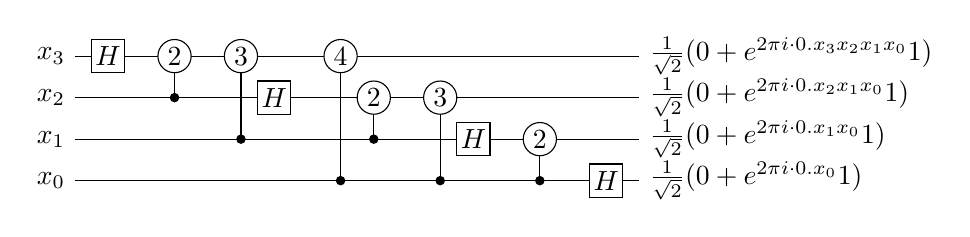
\begin{tikzpicture}[scale=1.000000,x=1pt,y=1pt]
\filldraw[color=white] (0.000000, -7.500000) rectangle (204.000000, 52.500000);
% Drawing wires
% Line 2: a3 W \ket{x_3} \frac{1}{\sqrt{2}}(\ket{0}+e^{2{\pi}i{\cdot0}.x_3x_2x_1x_0}\ket{1})
\draw[color=black] (0.000000,45.000000) -- (204.000000,45.000000);
\draw[color=black] (0.000000,45.000000) node[left] {$\ket{x_3}$};
% Line 3: a2 W \ket{x_2} \frac{1}{\sqrt{2}}(\ket{0}+e^{2{\pi}i{\cdot0}.x_2x_1x_0}\ket{1})
\draw[color=black] (0.000000,30.000000) -- (204.000000,30.000000);
\draw[color=black] (0.000000,30.000000) node[left] {$\ket{x_2}$};
% Line 4: a1 W \ket{x_1} \frac{1}{\sqrt{2}}(\ket{0}+e^{2{\pi}i{\cdot0}.x_1x_0}\ket{1})
\draw[color=black] (0.000000,15.000000) -- (204.000000,15.000000);
\draw[color=black] (0.000000,15.000000) node[left] {$\ket{x_1}$};
% Line 5: a0 W \ket{x_0} \frac{1}{\sqrt{2}}(\ket{0}+e^{2{\pi}i{\cdot0}.x_0}\ket{1})
\draw[color=black] (0.000000,0.000000) -- (204.000000,0.000000);
\draw[color=black] (0.000000,0.000000) node[left] {$\ket{x_0}$};
% Done with wires; drawing gates
% Line 6: a3 H
\begin{scope}
\draw[fill=white] (12.000000, 45.000000) +(-45.000000:8.485281pt and 8.485281pt) -- +(45.000000:8.485281pt and 8.485281pt) -- +(135.000000:8.485281pt and 8.485281pt) -- +(225.000000:8.485281pt and 8.485281pt) -- cycle;
\clip (12.000000, 45.000000) +(-45.000000:8.485281pt and 8.485281pt) -- +(45.000000:8.485281pt and 8.485281pt) -- +(135.000000:8.485281pt and 8.485281pt) -- +(225.000000:8.485281pt and 8.485281pt) -- cycle;
\draw (12.000000, 45.000000) node {$H$};
\end{scope}
% Line 7: a3 P $2$ a2
\draw (36.000000,45.000000) -- (36.000000,30.000000);
\begin{scope}
\draw[fill=white] (36.000000, 45.000000) circle(6.000000pt);
\clip (36.000000, 45.000000) circle(6.000000pt);
\draw (36.000000, 45.000000) node {$2$};
\end{scope}
\filldraw (36.000000, 30.000000) circle(1.500000pt);
% Line 8: a3 P $3$ a1
\draw (60.000000,45.000000) -- (60.000000,15.000000);
\begin{scope}
\draw[fill=white] (60.000000, 45.000000) circle(6.000000pt);
\clip (60.000000, 45.000000) circle(6.000000pt);
\draw (60.000000, 45.000000) node {$3$};
\end{scope}
\filldraw (60.000000, 15.000000) circle(1.500000pt);
% Line 10: a2 H
\begin{scope}
\draw[fill=white] (72.000000, 30.000000) +(-45.000000:8.485281pt and 8.485281pt) -- +(45.000000:8.485281pt and 8.485281pt) -- +(135.000000:8.485281pt and 8.485281pt) -- +(225.000000:8.485281pt and 8.485281pt) -- cycle;
\clip (72.000000, 30.000000) +(-45.000000:8.485281pt and 8.485281pt) -- +(45.000000:8.485281pt and 8.485281pt) -- +(135.000000:8.485281pt and 8.485281pt) -- +(225.000000:8.485281pt and 8.485281pt) -- cycle;
\draw (72.000000, 30.000000) node {$H$};
\end{scope}
% Line 9: a3 P $4$ a0
\draw (96.000000,45.000000) -- (96.000000,0.000000);
\begin{scope}
\draw[fill=white] (96.000000, 45.000000) circle(6.000000pt);
\clip (96.000000, 45.000000) circle(6.000000pt);
\draw (96.000000, 45.000000) node {$4$};
\end{scope}
\filldraw (96.000000, 0.000000) circle(1.500000pt);
% Line 11: a2 P $2$ a1
\draw (108.000000,30.000000) -- (108.000000,15.000000);
\begin{scope}
\draw[fill=white] (108.000000, 30.000000) circle(6.000000pt);
\clip (108.000000, 30.000000) circle(6.000000pt);
\draw (108.000000, 30.000000) node {$2$};
\end{scope}
\filldraw (108.000000, 15.000000) circle(1.500000pt);
% Line 12: a2 P $3$ a0
\draw (132.000000,30.000000) -- (132.000000,0.000000);
\begin{scope}
\draw[fill=white] (132.000000, 30.000000) circle(6.000000pt);
\clip (132.000000, 30.000000) circle(6.000000pt);
\draw (132.000000, 30.000000) node {$3$};
\end{scope}
\filldraw (132.000000, 0.000000) circle(1.500000pt);
% Line 13: a1 H
\begin{scope}
\draw[fill=white] (144.000000, 15.000000) +(-45.000000:8.485281pt and 8.485281pt) -- +(45.000000:8.485281pt and 8.485281pt) -- +(135.000000:8.485281pt and 8.485281pt) -- +(225.000000:8.485281pt and 8.485281pt) -- cycle;
\clip (144.000000, 15.000000) +(-45.000000:8.485281pt and 8.485281pt) -- +(45.000000:8.485281pt and 8.485281pt) -- +(135.000000:8.485281pt and 8.485281pt) -- +(225.000000:8.485281pt and 8.485281pt) -- cycle;
\draw (144.000000, 15.000000) node {$H$};
\end{scope}
% Line 14: a1 P $2$ a0
\draw (168.000000,15.000000) -- (168.000000,0.000000);
\begin{scope}
\draw[fill=white] (168.000000, 15.000000) circle(6.000000pt);
\clip (168.000000, 15.000000) circle(6.000000pt);
\draw (168.000000, 15.000000) node {$2$};
\end{scope}
\filldraw (168.000000, 0.000000) circle(1.500000pt);
% Line 15: a0 H
\begin{scope}
\draw[fill=white] (192.000000, -0.000000) +(-45.000000:8.485281pt and 8.485281pt) -- +(45.000000:8.485281pt and 8.485281pt) -- +(135.000000:8.485281pt and 8.485281pt) -- +(225.000000:8.485281pt and 8.485281pt) -- cycle;
\clip (192.000000, -0.000000) +(-45.000000:8.485281pt and 8.485281pt) -- +(45.000000:8.485281pt and 8.485281pt) -- +(135.000000:8.485281pt and 8.485281pt) -- +(225.000000:8.485281pt and 8.485281pt) -- cycle;
\draw (192.000000, -0.000000) node {$H$};
\end{scope}
% Done with gates; drawing ending labels
\draw[color=black] (204.000000,45.000000) node[right] {$\frac{1}{\sqrt{2}}(\ket{0}+e^{2{\pi}i{\cdot0}.x_3x_2x_1x_0}\ket{1})$};
\draw[color=black] (204.000000,30.000000) node[right] {$\frac{1}{\sqrt{2}}(\ket{0}+e^{2{\pi}i{\cdot0}.x_2x_1x_0}\ket{1})$};
\draw[color=black] (204.000000,15.000000) node[right] {$\frac{1}{\sqrt{2}}(\ket{0}+e^{2{\pi}i{\cdot0}.x_1x_0}\ket{1})$};
\draw[color=black] (204.000000,0.000000) node[right] {$\frac{1}{\sqrt{2}}(\ket{0}+e^{2{\pi}i{\cdot0}.x_0}\ket{1})$};
% Done with ending labels; drawing cut lines and comments
% Done with comments
\end{tikzpicture}

\end{figure}

\SaveVerb{name}|QFT4vert|
\begin{figure}[ht]
\caption{\protect\UseVerb{name}}
\providecommand{\ket}[1]{\left|#1\right\rangle}
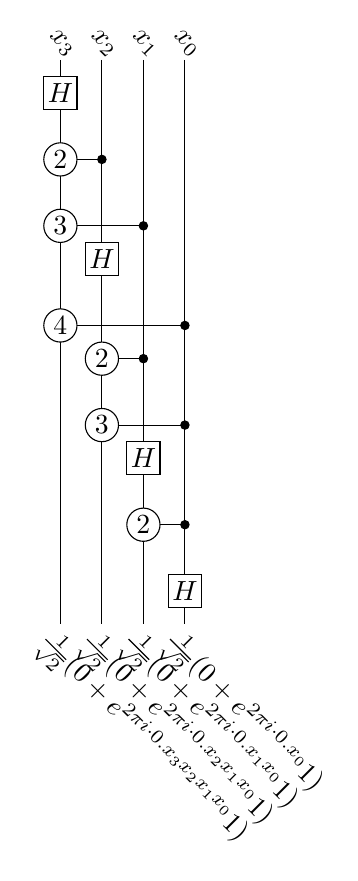
\begin{tikzpicture}[scale=1.000000,x=1pt,y=1pt]
\filldraw[color=white] (7.500000, 0.000000) rectangle (-52.500000, -204.000000);
% Drawing wires
% Line 3: a3 W \ket{x_3} \frac{1}{\sqrt{2}}(\ket{0}+e^{2{\pi}i{\cdot0}.x_3x_2x_1x_0}\ket{1})
\draw[color=black] (-45.000000,0.000000) -- (-45.000000,-204.000000);
\draw[color=black] (-45.000000,0.000000) node[above,anchor=south east,xshift=2pt,inner sep=0pt,rotate=-45] {$\ket{x_3}$};
% Line 4: a2 W \ket{x_2} \frac{1}{\sqrt{2}}(\ket{0}+e^{2{\pi}i{\cdot0}.x_2x_1x_0}\ket{1})
\draw[color=black] (-30.000000,0.000000) -- (-30.000000,-204.000000);
\draw[color=black] (-30.000000,0.000000) node[above,anchor=south east,xshift=2pt,inner sep=0pt,rotate=-45] {$\ket{x_2}$};
% Line 5: a1 W \ket{x_1} \frac{1}{\sqrt{2}}(\ket{0}+e^{2{\pi}i{\cdot0}.x_1x_0}\ket{1})
\draw[color=black] (-15.000000,0.000000) -- (-15.000000,-204.000000);
\draw[color=black] (-15.000000,0.000000) node[above,anchor=south east,xshift=2pt,inner sep=0pt,rotate=-45] {$\ket{x_1}$};
% Line 6: a0 W \ket{x_0} \frac{1}{\sqrt{2}}(\ket{0}+e^{2{\pi}i{\cdot0}.x_0}\ket{1})
\draw[color=black] (-0.000000,0.000000) -- (-0.000000,-204.000000);
\draw[color=black] (-0.000000,0.000000) node[above,anchor=south east,xshift=2pt,inner sep=0pt,rotate=-45] {$\ket{x_0}$};
% Done with wires; drawing gates
% Line 7: a3 H
\begin{scope}
\draw[fill=white] (-45.000000, -12.000000) +(-45.000000:8.485281pt and 8.485281pt) -- +(45.000000:8.485281pt and 8.485281pt) -- +(135.000000:8.485281pt and 8.485281pt) -- +(225.000000:8.485281pt and 8.485281pt) -- cycle;
\clip (-45.000000, -12.000000) +(-45.000000:8.485281pt and 8.485281pt) -- +(45.000000:8.485281pt and 8.485281pt) -- +(135.000000:8.485281pt and 8.485281pt) -- +(225.000000:8.485281pt and 8.485281pt) -- cycle;
\draw (-45.000000, -12.000000) node {$H$};
\end{scope}
% Line 8: a3 P $2$ a2
\draw (-45.000000,-36.000000) -- (-30.000000,-36.000000);
\begin{scope}
\draw[fill=white] (-45.000000, -36.000000) circle(6.000000pt);
\clip (-45.000000, -36.000000) circle(6.000000pt);
\draw (-45.000000, -36.000000) node {$2$};
\end{scope}
\filldraw (-30.000000, -36.000000) circle(1.500000pt);
% Line 9: a3 P $3$ a1
\draw (-45.000000,-60.000000) -- (-15.000000,-60.000000);
\begin{scope}
\draw[fill=white] (-45.000000, -60.000000) circle(6.000000pt);
\clip (-45.000000, -60.000000) circle(6.000000pt);
\draw (-45.000000, -60.000000) node {$3$};
\end{scope}
\filldraw (-15.000000, -60.000000) circle(1.500000pt);
% Line 11: a2 H
\begin{scope}
\draw[fill=white] (-30.000000, -72.000000) +(-45.000000:8.485281pt and 8.485281pt) -- +(45.000000:8.485281pt and 8.485281pt) -- +(135.000000:8.485281pt and 8.485281pt) -- +(225.000000:8.485281pt and 8.485281pt) -- cycle;
\clip (-30.000000, -72.000000) +(-45.000000:8.485281pt and 8.485281pt) -- +(45.000000:8.485281pt and 8.485281pt) -- +(135.000000:8.485281pt and 8.485281pt) -- +(225.000000:8.485281pt and 8.485281pt) -- cycle;
\draw (-30.000000, -72.000000) node {$H$};
\end{scope}
% Line 10: a3 P $4$ a0
\draw (-45.000000,-96.000000) -- (-0.000000,-96.000000);
\begin{scope}
\draw[fill=white] (-45.000000, -96.000000) circle(6.000000pt);
\clip (-45.000000, -96.000000) circle(6.000000pt);
\draw (-45.000000, -96.000000) node {$4$};
\end{scope}
\filldraw (-0.000000, -96.000000) circle(1.500000pt);
% Line 12: a2 P $2$ a1
\draw (-30.000000,-108.000000) -- (-15.000000,-108.000000);
\begin{scope}
\draw[fill=white] (-30.000000, -108.000000) circle(6.000000pt);
\clip (-30.000000, -108.000000) circle(6.000000pt);
\draw (-30.000000, -108.000000) node {$2$};
\end{scope}
\filldraw (-15.000000, -108.000000) circle(1.500000pt);
% Line 13: a2 P $3$ a0
\draw (-30.000000,-132.000000) -- (-0.000000,-132.000000);
\begin{scope}
\draw[fill=white] (-30.000000, -132.000000) circle(6.000000pt);
\clip (-30.000000, -132.000000) circle(6.000000pt);
\draw (-30.000000, -132.000000) node {$3$};
\end{scope}
\filldraw (-0.000000, -132.000000) circle(1.500000pt);
% Line 14: a1 H
\begin{scope}
\draw[fill=white] (-15.000000, -144.000000) +(-45.000000:8.485281pt and 8.485281pt) -- +(45.000000:8.485281pt and 8.485281pt) -- +(135.000000:8.485281pt and 8.485281pt) -- +(225.000000:8.485281pt and 8.485281pt) -- cycle;
\clip (-15.000000, -144.000000) +(-45.000000:8.485281pt and 8.485281pt) -- +(45.000000:8.485281pt and 8.485281pt) -- +(135.000000:8.485281pt and 8.485281pt) -- +(225.000000:8.485281pt and 8.485281pt) -- cycle;
\draw (-15.000000, -144.000000) node {$H$};
\end{scope}
% Line 15: a1 P $2$ a0
\draw (-15.000000,-168.000000) -- (-0.000000,-168.000000);
\begin{scope}
\draw[fill=white] (-15.000000, -168.000000) circle(6.000000pt);
\clip (-15.000000, -168.000000) circle(6.000000pt);
\draw (-15.000000, -168.000000) node {$2$};
\end{scope}
\filldraw (-0.000000, -168.000000) circle(1.500000pt);
% Line 16: a0 H
\begin{scope}
\draw[fill=white] (0.000000, -192.000000) +(-45.000000:8.485281pt and 8.485281pt) -- +(45.000000:8.485281pt and 8.485281pt) -- +(135.000000:8.485281pt and 8.485281pt) -- +(225.000000:8.485281pt and 8.485281pt) -- cycle;
\clip (0.000000, -192.000000) +(-45.000000:8.485281pt and 8.485281pt) -- +(45.000000:8.485281pt and 8.485281pt) -- +(135.000000:8.485281pt and 8.485281pt) -- +(225.000000:8.485281pt and 8.485281pt) -- cycle;
\draw (0.000000, -192.000000) node {$H$};
\end{scope}
% Done with gates; drawing ending labels
\draw[color=black] (-45.000000,-204.000000) node[below,anchor=north west,xshift=-2pt,inner sep=0pt,rotate=-45] {$\frac{1}{\sqrt{2}}(\ket{0}+e^{2{\pi}i{\cdot0}.x_3x_2x_1x_0}\ket{1})$};
\draw[color=black] (-30.000000,-204.000000) node[below,anchor=north west,xshift=-2pt,inner sep=0pt,rotate=-45] {$\frac{1}{\sqrt{2}}(\ket{0}+e^{2{\pi}i{\cdot0}.x_2x_1x_0}\ket{1})$};
\draw[color=black] (-15.000000,-204.000000) node[below,anchor=north west,xshift=-2pt,inner sep=0pt,rotate=-45] {$\frac{1}{\sqrt{2}}(\ket{0}+e^{2{\pi}i{\cdot0}.x_1x_0}\ket{1})$};
\draw[color=black] (-0.000000,-204.000000) node[below,anchor=north west,xshift=-2pt,inner sep=0pt,rotate=-45] {$\frac{1}{\sqrt{2}}(\ket{0}+e^{2{\pi}i{\cdot0}.x_0}\ket{1})$};
% Done with ending labels; drawing cut lines and comments
% Done with comments
\end{tikzpicture}

\end{figure}
\clearpage

\SaveVerb{name}|QuantumTeleportation|
\begin{figure}[ht]
\caption{\protect\UseVerb{name}}
\providecommand{\K}[1]{\left|#1\right\rangle}
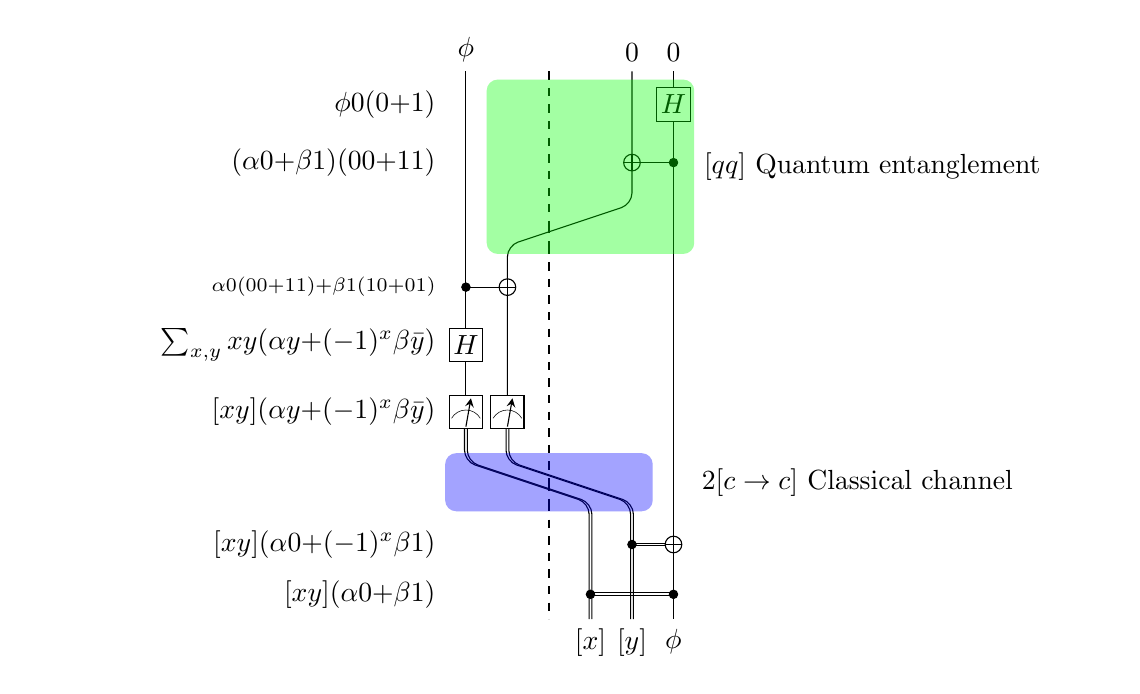
\begin{tikzpicture}[scale=1.000000,x=1pt,y=1pt]
\filldraw[color=white] (7.500000, 0.000000) rectangle (-82.500000, -198.000000);
% Drawing wires
% Line 2: a  W \K{\phi} [x]
\draw[color=black] (-75.000000,0.000000) -- (-75.000000,-123.000000);
\draw[color=black,rounded corners=4.000000pt] (-74.500000,-123.000000) -- (-74.500000,-141.000000) -- (-52.000000,-148.500000);
\draw[color=black,rounded corners=4.000000pt] (-75.500000,-123.000000) -- (-75.500000,-141.000000) -- (-53.000000,-148.500000);
\draw[color=black,rounded corners=4.000000pt] (-52.000000,-148.500000) -- (-29.500000,-156.000000) -- (-29.500000,-198.000000);
\draw[color=black,rounded corners=4.000000pt] (-53.000000,-148.500000) -- (-30.500000,-156.000000) -- (-30.500000,-198.000000);
\draw[color=black] (-75.000000,0.000000) node[above] {$\K{\phi}$};
% Line 3: x1 W type=o # Empty wire used for positioning
% Line 4: x0 W style=dashed # Dividing line
\draw[color=black,dashed] (-45.000000,0.000000) -- (-45.000000,-48.000000);
\draw[color=black,dashed] (-45.000000,-48.000000) -- (-45.000000,-55.500000);
\draw[color=black,dashed] (-45.000000,-55.500000) -- (-45.000000,-63.000000);
\draw[color=black,dashed] (-45.000000,-63.000000) -- (-45.000000,-141.000000);
\draw[color=black,dashed] (-45.000000,-141.000000) -- (-45.000000,-148.500000);
\draw[color=black,dashed] (-45.000000,-148.500000) -- (-45.000000,-156.000000);
\draw[color=black,dashed] (-45.000000,-156.000000) -- (-45.000000,-198.000000);
% Line 5: x2 W type=o # Empty wire used for positioning
% Line 6: b0 W \K{0} [y]
\draw[color=black,rounded corners=4.000000pt] (-15.000000,0.000000) -- (-15.000000,-48.000000) -- (-37.500000,-55.500000);
\draw[color=black,rounded corners=4.000000pt] (-37.500000,-55.500000) -- (-60.000000,-63.000000) -- (-60.000000,-123.000000);
\draw[color=black,rounded corners=4.000000pt] (-59.500000,-123.000000) -- (-59.500000,-141.000000) -- (-37.000000,-148.500000);
\draw[color=black,rounded corners=4.000000pt] (-60.500000,-123.000000) -- (-60.500000,-141.000000) -- (-38.000000,-148.500000);
\draw[color=black,rounded corners=4.000000pt] (-37.000000,-148.500000) -- (-14.500000,-156.000000) -- (-14.500000,-198.000000);
\draw[color=black,rounded corners=4.000000pt] (-38.000000,-148.500000) -- (-15.500000,-156.000000) -- (-15.500000,-198.000000);
\draw[color=black] (-15.000000,0.000000) node[above] {$\K{0}$};
% Line 7: b1 W \K{0} \K{\phi}
\draw[color=black] (-0.000000,0.000000) -- (-0.000000,-198.000000);
\draw[color=black] (-0.000000,0.000000) node[above] {$\K{0}$};
% Done with wires; drawing gates
% Line 10: b1 H    % $\K{\phi}\K{0}(\K{0}{+}\K{1})$
\draw (-82.500000, -12.000000) node[text width=144pt,left,text ragged left] {$\K{\phi}\K{0}(\K{0}{+}\K{1})$};
\begin{scope}
\draw[fill=white] (0.000000, -12.000000) +(-45.000000:8.485281pt and 8.485281pt) -- +(45.000000:8.485281pt and 8.485281pt) -- +(135.000000:8.485281pt and 8.485281pt) -- +(225.000000:8.485281pt and 8.485281pt) -- cycle;
\clip (0.000000, -12.000000) +(-45.000000:8.485281pt and 8.485281pt) -- +(45.000000:8.485281pt and 8.485281pt) -- +(135.000000:8.485281pt and 8.485281pt) -- +(225.000000:8.485281pt and 8.485281pt) -- cycle;
\draw (0.000000, -12.000000) node {$H$};
\end{scope}
% Line 11: +b0 b1   % $(\alpha\K{0}{+}\beta\K{1})(\K{00}{+}\K{11})$
\draw (-82.500000, -33.000000) node[text width=144pt,left,text ragged left] {$(\alpha\K{0}{+}\beta\K{1})(\K{00}{+}\K{11})$};
\draw (-15.000000,-33.000000) -- (-0.000000,-33.000000);
\begin{scope}
\draw[fill=white] (-15.000000, -33.000000) circle(3.000000pt);
\clip (-15.000000, -33.000000) circle(3.000000pt);
\draw (-18.000000, -33.000000) -- (-12.000000, -33.000000);
\draw (-15.000000, -36.000000) -- (-15.000000, -30.000000);
\end{scope}
\filldraw (-0.000000, -33.000000) circle(1.500000pt);
% Line 12: b0 x1 PERMUTE
% Line 13: +b0 a %$\scriptstyle\alpha\K{0}(\K{00}{+}\K{11}){+}\beta\K{1}(\K{10}{+}\K{01})$
\draw (-82.500000, -78.000000) node[text width=144pt,left,text ragged left] {$\scriptstyle\alpha\K{0}(\K{00}{+}\K{11}){+}\beta\K{1}(\K{10}{+}\K{01})$};
\draw (-75.000000,-78.000000) -- (-60.000000,-78.000000);
\begin{scope}
\draw[fill=white] (-60.000000, -78.000000) circle(3.000000pt);
\clip (-60.000000, -78.000000) circle(3.000000pt);
\draw (-63.000000, -78.000000) -- (-57.000000, -78.000000);
\draw (-60.000000, -81.000000) -- (-60.000000, -75.000000);
\end{scope}
\filldraw (-75.000000, -78.000000) circle(1.500000pt);
% Line 14: a H     % $\sum_{x,y}\K{xy}(\alpha\K{y}{+}(-1)^x\beta\K{\bar{y}})$
\draw (-82.500000, -99.000000) node[text width=144pt,left,text ragged left] {$\sum_{x,y}\K{xy}(\alpha\K{y}{+}(-1)^x\beta\K{\bar{y}})$};
\begin{scope}
\draw[fill=white] (-75.000000, -99.000000) +(-45.000000:8.485281pt and 8.485281pt) -- +(45.000000:8.485281pt and 8.485281pt) -- +(135.000000:8.485281pt and 8.485281pt) -- +(225.000000:8.485281pt and 8.485281pt) -- cycle;
\clip (-75.000000, -99.000000) +(-45.000000:8.485281pt and 8.485281pt) -- +(45.000000:8.485281pt and 8.485281pt) -- +(135.000000:8.485281pt and 8.485281pt) -- +(225.000000:8.485281pt and 8.485281pt) -- cycle;
\draw (-75.000000, -99.000000) node {$H$};
\end{scope}
% Line 15: a b0 M  % $[xy](\alpha\K{y}{+}(-1)^x\beta\K{\bar{y}})$
\draw (-82.500000, -123.000000) node[text width=144pt,left,text ragged left] {$[xy](\alpha\K{y}{+}(-1)^x\beta\K{\bar{y}})$};
\draw[fill=white] (-81.000000, -129.000000) rectangle (-69.000000, -117.000000);
\draw[very thin] (-75.000000, -122.400000) arc (90:150:6.000000pt);
\draw[very thin] (-75.000000, -122.400000) arc (90:30:6.000000pt);
\draw[->,>=stealth] (-75.000000, -128.400000) -- +(80:10.392305pt);
\draw[fill=white] (-66.000000, -129.000000) rectangle (-54.000000, -117.000000);
\draw[very thin] (-60.000000, -122.400000) arc (90:150:6.000000pt);
\draw[very thin] (-60.000000, -122.400000) arc (90:30:6.000000pt);
\draw[->,>=stealth] (-60.000000, -128.400000) -- +(80:10.392305pt);
% Line 16: x1 x2 a b0 PERMUTE
% Line 17: +b1 b0   % $[xy](\alpha\K{0}{+}(-1)^x\beta\K{1})$
\draw (-82.500000, -171.000000) node[text width=144pt,left,text ragged left] {$[xy](\alpha\K{0}{+}(-1)^x\beta\K{1})$};
\draw (-15.000000,-170.500000) -- (-0.000000,-170.500000);
\draw (-15.000000,-171.500000) -- (-0.000000,-171.500000);
\begin{scope}
\draw[fill=white] (-0.000000, -171.000000) circle(3.000000pt);
\clip (-0.000000, -171.000000) circle(3.000000pt);
\draw (-3.000000, -171.000000) -- (3.000000, -171.000000);
\draw (-0.000000, -174.000000) -- (-0.000000, -168.000000);
\end{scope}
\filldraw (-15.000000, -171.000000) circle(1.500000pt);
% Line 18: b1 a  % $[xy](\alpha\K{0}{+}\beta\K{1})$
\draw (-82.500000, -189.000000) node[text width=144pt,left,text ragged left] {$[xy](\alpha\K{0}{+}\beta\K{1})$};
\draw (-30.000000,-188.500000) -- (-0.000000,-188.500000);
\draw (-30.000000,-189.500000) -- (-0.000000,-189.500000);
\filldraw (-0.000000, -189.000000) circle(1.500000pt);
\filldraw (-30.000000, -189.000000) circle(1.500000pt);
% Done with gates; drawing ending labels
\draw[color=black] (-30.000000,-198.000000) node[below] {$[x]$};
\draw[color=black] (-15.000000,-198.000000) node[below] {$[y]$};
\draw[color=black] (-0.000000,-198.000000) node[below] {$\K{\phi}$};
% Done with ending labels; drawing cut lines and comments
% Line 23: b0 b1 x1 x2 @ 0 2 qq %% $[qq]$ Quantum entanglement
\draw[draw opacity=0.000000,fill opacity=0.200000,fill=green,rounded corners] (-67.500000,-3.000000) rectangle (7.500000,-66.000000);
\draw (7.500000, -34.500000) node[text width=144pt,right] {$[qq]$ Quantum entanglement};
\draw[draw opacity=0.000000,fill opacity=0.200000,fill=green,rounded corners] (-67.500000,-3.000000) rectangle (7.500000,-66.000000);
% Line 24: a b0 x2 x1 @ 6 6 cc %% \hspace{.5cm}$2[c\rightarrow c]$ Classical channel
\draw[draw opacity=0.000000,fill opacity=0.200000,fill=blue,rounded corners] (-82.500000,-138.000000) rectangle (-7.500000,-159.000000);
\draw (-7.500000, -148.500000) node[text width=144pt,right] {\hspace{.5cm}$2[c\rightarrow c]$ Classical channel};
\draw[draw opacity=0.000000,fill opacity=0.200000,fill=blue,rounded corners] (-82.500000,-138.000000) rectangle (-7.500000,-159.000000);
% Done with comments
\end{tikzpicture}

\end{figure}

\SaveVerb{name}|RecursiveQFT|
\begin{figure}[ht]
\caption{\protect\UseVerb{name}}
\newcommand{\ket}[1]{\left| #1 \right\rangle}
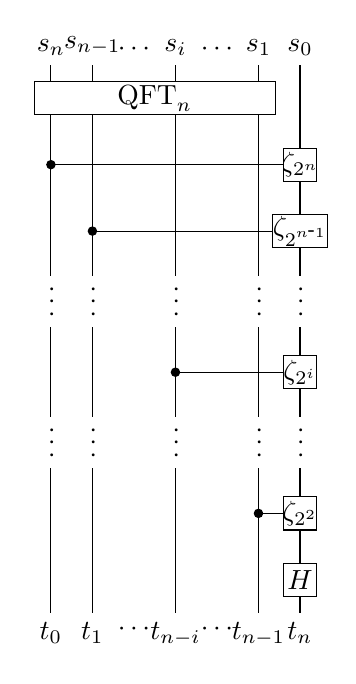
\begin{tikzpicture}[scale=1.000000,x=1pt,y=1pt]
\filldraw[color=white] (7.500000, 0.000000) rectangle (-97.500000, -198.000000);
% Drawing wires
% Line 3: n W s_{n} t_0
\draw[color=black] (-90.000000,0.000000) -- (-90.000000,-198.000000);
\draw[color=black] (-90.000000,0.000000) node[above] {$s_{n}$};
% Line 4: n-1 W s_{n-1} t_1
\draw[color=black] (-75.000000,0.000000) -- (-75.000000,-198.000000);
\draw[color=black] (-75.000000,0.000000) node[above] {$s_{n-1}$};
% Line 5: ...1 W
\draw[color=black] (-60.000000,0.000000) node[above] {$\cdots$};
% Line 6: i W s_{i} t_{n-i}
\draw[color=black] (-45.000000,0.000000) -- (-45.000000,-198.000000);
\draw[color=black] (-45.000000,0.000000) node[above] {$s_{i}$};
% Line 7: ...2 W
\draw[color=black] (-30.000000,0.000000) node[above] {$\cdots$};
% Line 8: 1 W s_1 t_{n-1}
\draw[color=black] (-15.000000,0.000000) -- (-15.000000,-198.000000);
\draw[color=black] (-15.000000,0.000000) node[above] {$s_1$};
% Line 9: 0 W s_0 t_{n}
\draw[color=black] (-0.000000,0.000000) -- (-0.000000,-198.000000);
\draw[color=black] (-0.000000,0.000000) node[above] {$s_0$};
% Done with wires; drawing gates
% Line 11: n n-1 ...1 i 1 G $\hbox{QFT}_{n}$ width=40
\draw (-90.000000,-12.000000) -- (-15.000000,-12.000000);
\begin{scope}
\draw[fill=white] (-52.500000, -12.000000) +(-45.000000:61.518290pt and 8.485281pt) -- +(45.000000:61.518290pt and 8.485281pt) -- +(135.000000:61.518290pt and 8.485281pt) -- +(225.000000:61.518290pt and 8.485281pt) -- cycle;
\clip (-52.500000, -12.000000) +(-45.000000:61.518290pt and 8.485281pt) -- +(45.000000:61.518290pt and 8.485281pt) -- +(135.000000:61.518290pt and 8.485281pt) -- +(225.000000:61.518290pt and 8.485281pt) -- cycle;
\draw (-52.500000, -12.000000) node {$\hbox{QFT}_{n}$};
\end{scope}
% Line 12: 0 G $\zeta_{2^n}$ n
\draw (-90.000000,-36.000000) -- (-0.000000,-36.000000);
\begin{scope}
\draw[fill=white] (0.000000, -36.000000) +(-45.000000:8.485281pt and 8.485281pt) -- +(45.000000:8.485281pt and 8.485281pt) -- +(135.000000:8.485281pt and 8.485281pt) -- +(225.000000:8.485281pt and 8.485281pt) -- cycle;
\clip (0.000000, -36.000000) +(-45.000000:8.485281pt and 8.485281pt) -- +(45.000000:8.485281pt and 8.485281pt) -- +(135.000000:8.485281pt and 8.485281pt) -- +(225.000000:8.485281pt and 8.485281pt) -- cycle;
\draw (0.000000, -36.000000) node {$\zeta_{2^n}$};
\end{scope}
\filldraw (-90.000000, -36.000000) circle(1.500000pt);
% Line 13: 0 G $\zeta_{\scriptstyle{}2^{n{\scalebox{.75}[1.0]{-}}1}}$ n-1 width=20
\draw (-75.000000,-60.000000) -- (-0.000000,-60.000000);
\begin{scope}
\draw[fill=white] (0.000000, -60.000000) +(-45.000000:14.142136pt and 8.485281pt) -- +(45.000000:14.142136pt and 8.485281pt) -- +(135.000000:14.142136pt and 8.485281pt) -- +(225.000000:14.142136pt and 8.485281pt) -- cycle;
\clip (0.000000, -60.000000) +(-45.000000:14.142136pt and 8.485281pt) -- +(45.000000:14.142136pt and 8.485281pt) -- +(135.000000:14.142136pt and 8.485281pt) -- +(225.000000:14.142136pt and 8.485281pt) -- cycle;
\draw (0.000000, -60.000000) node {$\zeta_{\scriptstyle{}2^{n{\scalebox{.75}[1.0]{-}}1}}$};
\end{scope}
\filldraw (-75.000000, -60.000000) circle(1.500000pt);
% Line 14: LABEL ...
\draw[color=black] (-90.000000, -85.500000) node [fill=white, rotate around={-90:(0,0)}] {$\cdots$};
\draw[color=black] (-75.000000, -85.500000) node [fill=white, rotate around={-90:(0,0)}] {$\cdots$};
\draw[color=black] (-45.000000, -85.500000) node [fill=white, rotate around={-90:(0,0)}] {$\cdots$};
\draw[color=black] (-15.000000, -85.500000) node [fill=white, rotate around={-90:(0,0)}] {$\cdots$};
\draw[color=black] (-0.000000, -85.500000) node [fill=white, rotate around={-90:(0,0)}] {$\cdots$};
% Line 15: 0 G $\zeta_{2^i}$ i
\draw (-45.000000,-111.000000) -- (-0.000000,-111.000000);
\begin{scope}
\draw[fill=white] (0.000000, -111.000000) +(-45.000000:8.485281pt and 8.485281pt) -- +(45.000000:8.485281pt and 8.485281pt) -- +(135.000000:8.485281pt and 8.485281pt) -- +(225.000000:8.485281pt and 8.485281pt) -- cycle;
\clip (0.000000, -111.000000) +(-45.000000:8.485281pt and 8.485281pt) -- +(45.000000:8.485281pt and 8.485281pt) -- +(135.000000:8.485281pt and 8.485281pt) -- +(225.000000:8.485281pt and 8.485281pt) -- cycle;
\draw (0.000000, -111.000000) node {$\zeta_{2^i}$};
\end{scope}
\filldraw (-45.000000, -111.000000) circle(1.500000pt);
% Line 16: LABEL ...
\draw[color=black] (-90.000000, -136.500000) node [fill=white, rotate around={-90:(0,0)}] {$\cdots$};
\draw[color=black] (-75.000000, -136.500000) node [fill=white, rotate around={-90:(0,0)}] {$\cdots$};
\draw[color=black] (-45.000000, -136.500000) node [fill=white, rotate around={-90:(0,0)}] {$\cdots$};
\draw[color=black] (-15.000000, -136.500000) node [fill=white, rotate around={-90:(0,0)}] {$\cdots$};
\draw[color=black] (-0.000000, -136.500000) node [fill=white, rotate around={-90:(0,0)}] {$\cdots$};
% Line 17: 0 G $\zeta_{2^2}$ 1
\draw (-15.000000,-162.000000) -- (-0.000000,-162.000000);
\begin{scope}
\draw[fill=white] (0.000000, -162.000000) +(-45.000000:8.485281pt and 8.485281pt) -- +(45.000000:8.485281pt and 8.485281pt) -- +(135.000000:8.485281pt and 8.485281pt) -- +(225.000000:8.485281pt and 8.485281pt) -- cycle;
\clip (0.000000, -162.000000) +(-45.000000:8.485281pt and 8.485281pt) -- +(45.000000:8.485281pt and 8.485281pt) -- +(135.000000:8.485281pt and 8.485281pt) -- +(225.000000:8.485281pt and 8.485281pt) -- cycle;
\draw (0.000000, -162.000000) node {$\zeta_{2^2}$};
\end{scope}
\filldraw (-15.000000, -162.000000) circle(1.500000pt);
% Line 18: 0 H
\begin{scope}
\draw[fill=white] (0.000000, -186.000000) +(-45.000000:8.485281pt and 8.485281pt) -- +(45.000000:8.485281pt and 8.485281pt) -- +(135.000000:8.485281pt and 8.485281pt) -- +(225.000000:8.485281pt and 8.485281pt) -- cycle;
\clip (0.000000, -186.000000) +(-45.000000:8.485281pt and 8.485281pt) -- +(45.000000:8.485281pt and 8.485281pt) -- +(135.000000:8.485281pt and 8.485281pt) -- +(225.000000:8.485281pt and 8.485281pt) -- cycle;
\draw (0.000000, -186.000000) node {$H$};
\end{scope}
% Done with gates; drawing ending labels
\draw[color=black] (-90.000000,-198.000000) node[below] {$t_0$};
\draw[color=black] (-75.000000,-198.000000) node[below] {$t_1$};
\draw[color=black] (-60.000000,-198.000000) node[below] {$\cdots$};
\draw[color=black] (-45.000000,-198.000000) node[below] {$t_{n-i}$};
\draw[color=black] (-30.000000,-198.000000) node[below] {$\cdots$};
\draw[color=black] (-15.000000,-198.000000) node[below] {$t_{n-1}$};
\draw[color=black] (-0.000000,-198.000000) node[below] {$t_{n}$};
% Done with ending labels; drawing cut lines and comments
% Done with comments
\end{tikzpicture}

\end{figure}

\SaveVerb{name}|RecursiveQFTv2|
\begin{figure}[ht]
\caption{\protect\UseVerb{name}}
\newcommand{\ket}[1]{\left| #1 \right\rangle}
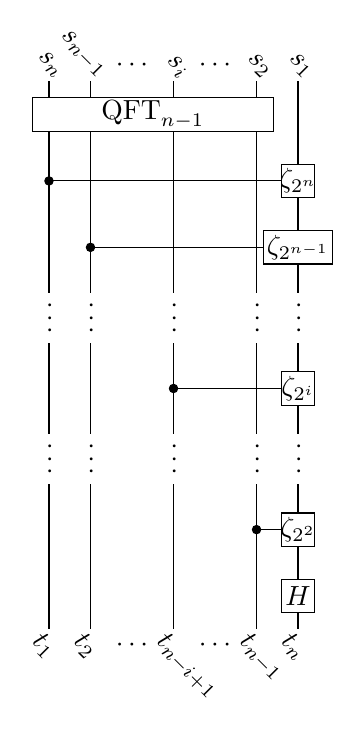
\begin{tikzpicture}[scale=1.000000,x=1pt,y=1pt]
\filldraw[color=white] (7.500000, 0.000000) rectangle (-97.500000, -198.000000);
% Drawing wires
% Line 2: n W \ket{s_n} \ket{t_1}
\draw[color=black] (-90.000000,0.000000) -- (-90.000000,-198.000000);
\draw[color=black] (-90.000000,0.000000) node[above,anchor=south east,xshift=2pt,inner sep=0pt,rotate=-45] {$\ket{s_n}$};
% Line 3: n-1 W \ket{s_{n-1}} \ket{t_2}
\draw[color=black] (-75.000000,0.000000) -- (-75.000000,-198.000000);
\draw[color=black] (-75.000000,0.000000) node[above,anchor=south east,xshift=2pt,inner sep=0pt,rotate=-45] {$\ket{s_{n-1}}$};
% Line 4: ...1 W
\draw[color=black] (-60.000000,0.000000) node[above] {$\cdots$};
% Line 5: i W \ket{s_{i}} \ket{t_{n-i+1}}
\draw[color=black] (-45.000000,0.000000) -- (-45.000000,-198.000000);
\draw[color=black] (-45.000000,0.000000) node[above,anchor=south east,xshift=2pt,inner sep=0pt,rotate=-45] {$\ket{s_{i}}$};
% Line 6: ...2 W
\draw[color=black] (-30.000000,0.000000) node[above] {$\cdots$};
% Line 7: 2 W \ket{s_2} \ket{t_{n-1}}
\draw[color=black] (-15.000000,0.000000) -- (-15.000000,-198.000000);
\draw[color=black] (-15.000000,0.000000) node[above,anchor=south east,xshift=2pt,inner sep=0pt,rotate=-45] {$\ket{s_2}$};
% Line 8: 1 W \ket{s_1} \ket{t_{n}}
\draw[color=black] (-0.000000,0.000000) -- (-0.000000,-198.000000);
\draw[color=black] (-0.000000,0.000000) node[above,anchor=south east,xshift=2pt,inner sep=0pt,rotate=-45] {$\ket{s_1}$};
% Done with wires; drawing gates
% Line 11: n n-1 ...1 i 2 G $\hbox{QFT}_{n-1}$ width=40
\draw (-90.000000,-12.000000) -- (-15.000000,-12.000000);
\begin{scope}
\draw[fill=white] (-52.500000, -12.000000) +(-45.000000:61.518290pt and 8.485281pt) -- +(45.000000:61.518290pt and 8.485281pt) -- +(135.000000:61.518290pt and 8.485281pt) -- +(225.000000:61.518290pt and 8.485281pt) -- cycle;
\clip (-52.500000, -12.000000) +(-45.000000:61.518290pt and 8.485281pt) -- +(45.000000:61.518290pt and 8.485281pt) -- +(135.000000:61.518290pt and 8.485281pt) -- +(225.000000:61.518290pt and 8.485281pt) -- cycle;
\draw (-52.500000, -12.000000) node {$\hbox{QFT}_{n-1}$};
\end{scope}
% Line 12: 1 G $\zeta_{2^n}$ n
\draw (-90.000000,-36.000000) -- (-0.000000,-36.000000);
\begin{scope}
\draw[fill=white] (0.000000, -36.000000) +(-45.000000:8.485281pt and 8.485281pt) -- +(45.000000:8.485281pt and 8.485281pt) -- +(135.000000:8.485281pt and 8.485281pt) -- +(225.000000:8.485281pt and 8.485281pt) -- cycle;
\clip (0.000000, -36.000000) +(-45.000000:8.485281pt and 8.485281pt) -- +(45.000000:8.485281pt and 8.485281pt) -- +(135.000000:8.485281pt and 8.485281pt) -- +(225.000000:8.485281pt and 8.485281pt) -- cycle;
\draw (0.000000, -36.000000) node {$\zeta_{2^n}$};
\end{scope}
\filldraw (-90.000000, -36.000000) circle(1.500000pt);
% Line 13: 1 G $\zeta_{2^{n-1}}$ n-1 width=25
\draw (-75.000000,-60.000000) -- (-0.000000,-60.000000);
\begin{scope}
\draw[fill=white] (0.000000, -60.000000) +(-45.000000:17.677670pt and 8.485281pt) -- +(45.000000:17.677670pt and 8.485281pt) -- +(135.000000:17.677670pt and 8.485281pt) -- +(225.000000:17.677670pt and 8.485281pt) -- cycle;
\clip (0.000000, -60.000000) +(-45.000000:17.677670pt and 8.485281pt) -- +(45.000000:17.677670pt and 8.485281pt) -- +(135.000000:17.677670pt and 8.485281pt) -- +(225.000000:17.677670pt and 8.485281pt) -- cycle;
\draw (0.000000, -60.000000) node {$\zeta_{2^{n-1}}$};
\end{scope}
\filldraw (-75.000000, -60.000000) circle(1.500000pt);
% Line 14: LABEL ...
\draw[color=black] (-90.000000, -85.500000) node [fill=white, rotate around={-90:(0,0)}] {$\cdots$};
\draw[color=black] (-75.000000, -85.500000) node [fill=white, rotate around={-90:(0,0)}] {$\cdots$};
\draw[color=black] (-45.000000, -85.500000) node [fill=white, rotate around={-90:(0,0)}] {$\cdots$};
\draw[color=black] (-15.000000, -85.500000) node [fill=white, rotate around={-90:(0,0)}] {$\cdots$};
\draw[color=black] (-0.000000, -85.500000) node [fill=white, rotate around={-90:(0,0)}] {$\cdots$};
% Line 15: 1 G $\zeta_{2^i}$ i
\draw (-45.000000,-111.000000) -- (-0.000000,-111.000000);
\begin{scope}
\draw[fill=white] (0.000000, -111.000000) +(-45.000000:8.485281pt and 8.485281pt) -- +(45.000000:8.485281pt and 8.485281pt) -- +(135.000000:8.485281pt and 8.485281pt) -- +(225.000000:8.485281pt and 8.485281pt) -- cycle;
\clip (0.000000, -111.000000) +(-45.000000:8.485281pt and 8.485281pt) -- +(45.000000:8.485281pt and 8.485281pt) -- +(135.000000:8.485281pt and 8.485281pt) -- +(225.000000:8.485281pt and 8.485281pt) -- cycle;
\draw (0.000000, -111.000000) node {$\zeta_{2^i}$};
\end{scope}
\filldraw (-45.000000, -111.000000) circle(1.500000pt);
% Line 16: LABEL ...
\draw[color=black] (-90.000000, -136.500000) node [fill=white, rotate around={-90:(0,0)}] {$\cdots$};
\draw[color=black] (-75.000000, -136.500000) node [fill=white, rotate around={-90:(0,0)}] {$\cdots$};
\draw[color=black] (-45.000000, -136.500000) node [fill=white, rotate around={-90:(0,0)}] {$\cdots$};
\draw[color=black] (-15.000000, -136.500000) node [fill=white, rotate around={-90:(0,0)}] {$\cdots$};
\draw[color=black] (-0.000000, -136.500000) node [fill=white, rotate around={-90:(0,0)}] {$\cdots$};
% Line 17: 1 G $\zeta_{2^2}$ 2
\draw (-15.000000,-162.000000) -- (-0.000000,-162.000000);
\begin{scope}
\draw[fill=white] (0.000000, -162.000000) +(-45.000000:8.485281pt and 8.485281pt) -- +(45.000000:8.485281pt and 8.485281pt) -- +(135.000000:8.485281pt and 8.485281pt) -- +(225.000000:8.485281pt and 8.485281pt) -- cycle;
\clip (0.000000, -162.000000) +(-45.000000:8.485281pt and 8.485281pt) -- +(45.000000:8.485281pt and 8.485281pt) -- +(135.000000:8.485281pt and 8.485281pt) -- +(225.000000:8.485281pt and 8.485281pt) -- cycle;
\draw (0.000000, -162.000000) node {$\zeta_{2^2}$};
\end{scope}
\filldraw (-15.000000, -162.000000) circle(1.500000pt);
% Line 18: 1 H
\begin{scope}
\draw[fill=white] (0.000000, -186.000000) +(-45.000000:8.485281pt and 8.485281pt) -- +(45.000000:8.485281pt and 8.485281pt) -- +(135.000000:8.485281pt and 8.485281pt) -- +(225.000000:8.485281pt and 8.485281pt) -- cycle;
\clip (0.000000, -186.000000) +(-45.000000:8.485281pt and 8.485281pt) -- +(45.000000:8.485281pt and 8.485281pt) -- +(135.000000:8.485281pt and 8.485281pt) -- +(225.000000:8.485281pt and 8.485281pt) -- cycle;
\draw (0.000000, -186.000000) node {$H$};
\end{scope}
% Done with gates; drawing ending labels
\draw[color=black] (-90.000000,-198.000000) node[below,anchor=north west,xshift=-2pt,inner sep=0pt,rotate=-45] {$\ket{t_1}$};
\draw[color=black] (-75.000000,-198.000000) node[below,anchor=north west,xshift=-2pt,inner sep=0pt,rotate=-45] {$\ket{t_2}$};
\draw[color=black] (-60.000000,-198.000000) node[below] {$\cdots$};
\draw[color=black] (-45.000000,-198.000000) node[below,anchor=north west,xshift=-2pt,inner sep=0pt,rotate=-45] {$\ket{t_{n-i+1}}$};
\draw[color=black] (-30.000000,-198.000000) node[below] {$\cdots$};
\draw[color=black] (-15.000000,-198.000000) node[below,anchor=north west,xshift=-2pt,inner sep=0pt,rotate=-45] {$\ket{t_{n-1}}$};
\draw[color=black] (-0.000000,-198.000000) node[below,anchor=north west,xshift=-2pt,inner sep=0pt,rotate=-45] {$\ket{t_{n}}$};
% Done with ending labels; drawing cut lines and comments
% Done with comments
\end{tikzpicture}

\end{figure}

\SaveVerb{name}|ShapeExamples|
\begin{figure}[ht]
\caption{\protect\UseVerb{name}}
%! \usetikzlibrary{decorations.pathreplacing,decorations.pathmorphing}
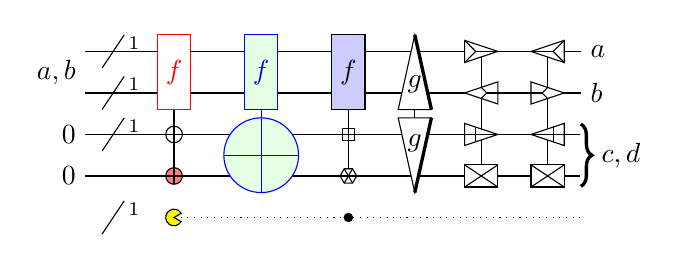
\begin{tikzpicture}[scale=1.000000,x=1pt,y=1pt]
\filldraw[color=white] (0.000000, -7.500000) rectangle (179.000000, 67.500000);
% Drawing wires
% Line 1: a b W a,b
\draw[color=black] (0.000000,60.000000) -- (179.000000,60.000000);
%   Deferring wire label at (0.000000,60.000000)
% Line 1: a b W a,b
\draw[color=black] (0.000000,45.000000) -- (179.000000,45.000000);
\draw[color=black] (0.000000,52.500000) node[left] {$a,b$};
% Line 2: c W 0
\draw[color=black] (0.000000,30.000000) -- (179.000000,30.000000);
\draw[color=black] (0.000000,30.000000) node[left] {$0$};
% Line 3: d W 0
\draw[color=black] (0.000000,15.000000) -- (179.000000,15.000000);
\draw[color=black] (0.000000,15.000000) node[left] {$0$};
% Line 4: x W owire
\draw[color=black,dotted] (32.000000,0.000000) -- (179.000000,0.000000);
% Done with wires; drawing gates
% Line 10: a b c x / 1
\draw (6.000000, 54.000000) -- (14.000000, 66.000000);
\draw (12.000000, 63.000000) node[right] {$\scriptstyle{1}$};
\draw (6.000000, 39.000000) -- (14.000000, 51.000000);
\draw (12.000000, 48.000000) node[right] {$\scriptstyle{1}$};
\draw (6.000000, 24.000000) -- (14.000000, 36.000000);
\draw (12.000000, 33.000000) node[right] {$\scriptstyle{1}$};
\draw (6.000000, -6.000000) -- (14.000000, 6.000000);
\draw (12.000000, 3.000000) node[right] {$\scriptstyle{1}$};
% Line 11: x:op="\draw[fill=yellow] (0,0) -- (30:3pt) arc (30:330:3pt) -- cycle;":sh=0:style=dotted:qwire
\begin{scope}
\begin{scope}[shift={(32.000000,0.000000)}]
\draw[fill=yellow] (0,0) -- (30:3pt) arc (30:330:3pt) -- cycle;
\end{scope}
\end{scope}
% Line 12: a b G:color=red $f$ +c +d:fill=red!50!white
\draw (32.000000,60.000000) -- (32.000000,15.000000);
\begin{scope}[color=red]
\begin{scope}
\draw[fill=white] (32.000000, 52.500000) +(-45.000000:8.485281pt and 19.091883pt) -- +(45.000000:8.485281pt and 19.091883pt) -- +(135.000000:8.485281pt and 19.091883pt) -- +(225.000000:8.485281pt and 19.091883pt) -- cycle;
\clip (32.000000, 52.500000) +(-45.000000:8.485281pt and 19.091883pt) -- +(45.000000:8.485281pt and 19.091883pt) -- +(135.000000:8.485281pt and 19.091883pt) -- +(225.000000:8.485281pt and 19.091883pt) -- cycle;
\draw (32.000000, 52.500000) node {$f$};
\end{scope}
\end{scope}
\begin{scope}
\draw[fill=white] (32.000000, 30.000000) circle(3.000000pt);
\clip (32.000000, 30.000000) circle(3.000000pt);
\draw (29.000000, 30.000000) -- (35.000000, 30.000000);
\draw (32.000000, 27.000000) -- (32.000000, 33.000000);
\end{scope}
\begin{scope}
\draw[fill=red!50!white] (32.000000, 15.000000) circle(3.000000pt);
\clip (32.000000, 15.000000) circle(3.000000pt);
\draw (29.000000, 15.000000) -- (35.000000, 15.000000);
\draw (32.000000, 12.000000) -- (32.000000, 18.000000);
\end{scope}
% Line 13: a b G $f$ c d P:size=27 + color=blue fi=green!10!white
\begin{scope}[color=blue]
\draw (63.500000,60.000000) -- (63.500000,15.000000);
\begin{scope}[color=blue]
\begin{scope}
\draw[fill=green!10!white] (63.500000, 52.500000) +(-45.000000:8.485281pt and 19.091883pt) -- +(45.000000:8.485281pt and 19.091883pt) -- +(135.000000:8.485281pt and 19.091883pt) -- +(225.000000:8.485281pt and 19.091883pt) -- cycle;
\clip (63.500000, 52.500000) +(-45.000000:8.485281pt and 19.091883pt) -- +(45.000000:8.485281pt and 19.091883pt) -- +(135.000000:8.485281pt and 19.091883pt) -- +(225.000000:8.485281pt and 19.091883pt) -- cycle;
\draw (63.500000, 52.500000) node {$f$};
\end{scope}
\end{scope}
\begin{scope}[color=blue]
\begin{scope}
\draw[fill=green!10!white] (63.500000, 22.500000) circle(13.500000pt);
\clip (63.500000, 22.500000) circle(13.500000pt);
\draw (50.000000, 22.500000) -- (77.000000, 22.500000);
\draw (63.500000, 9.000000) -- (63.500000, 36.000000);
\end{scope}
\end{scope}
\end{scope}
% Line 14: x TOUCH
% Line 15: a b G:op=$f$ +c:sh=box d:sh=6:op=* fi=blue!20!white
\draw (95.000000,60.000000) -- (95.000000,15.000000);
\begin{scope}
\draw[fill=blue!20!white] (95.000000, 52.500000) +(-45.000000:8.485281pt and 19.091883pt) -- +(45.000000:8.485281pt and 19.091883pt) -- +(135.000000:8.485281pt and 19.091883pt) -- +(225.000000:8.485281pt and 19.091883pt) -- cycle;
\clip (95.000000, 52.500000) +(-45.000000:8.485281pt and 19.091883pt) -- +(45.000000:8.485281pt and 19.091883pt) -- +(135.000000:8.485281pt and 19.091883pt) -- +(225.000000:8.485281pt and 19.091883pt) -- cycle;
\draw (95.000000, 52.500000) node {$f$};
\end{scope}
\begin{scope}
\draw[fill=white] (95.000000, 30.000000) +(-45.000000:3.000000pt) -- +(45.000000:3.000000pt) -- +(135.000000:3.000000pt) -- +(225.000000:3.000000pt) -- cycle;
\clip (95.000000, 30.000000) +(-45.000000:3.000000pt) -- +(45.000000:3.000000pt) -- +(135.000000:3.000000pt) -- +(225.000000:3.000000pt) -- cycle;
\draw (92.000000, 30.000000) -- (98.000000, 30.000000);
\draw (95.000000, 27.000000) -- (95.000000, 33.000000);
\end{scope}
\begin{scope}
\draw[fill=white] (95.000000, 15.000000) +(-60.000000:3.000000pt) -- +(0.000000:3.000000pt) -- +(60.000000:3.000000pt) -- +(120.000000:3.000000pt) -- +(180.000000:3.000000pt) -- +(240.000000:3.000000pt) -- cycle;
\clip (95.000000, 15.000000) +(-60.000000:3.000000pt) -- +(0.000000:3.000000pt) -- +(60.000000:3.000000pt) -- +(120.000000:3.000000pt) -- +(180.000000:3.000000pt) -- +(240.000000:3.000000pt) -- cycle;
\draw (95.000000, 15.000000) -- +(-60.000000:3.000000pt);
\draw (95.000000, 15.000000) -- +(0.000000:3.000000pt);
\draw (95.000000, 15.000000) -- +(60.000000:3.000000pt);
\draw (95.000000, 15.000000) -- +(120.000000:3.000000pt);
\draw (95.000000, 15.000000) -- +(180.000000:3.000000pt);
\draw (95.000000, 15.000000) -- +(240.000000:3.000000pt);
\end{scope}
% Line 17: x:sh=1
\filldraw (95.000000, 0.000000) circle(1.500000pt);
% Line 16: a b G|:shape=3 $g$ c d G|:shape=-3 $g$
\draw (119.000000,60.000000) -- (119.000000,15.000000);
\begin{scope}
\draw[fill=white] (119.000000, 48.000000) +(-30.000000:6.928203pt and 18.000000pt) -- +(90.000000:6.928203pt and 18.000000pt) -- +(210.000000:6.928203pt and 18.000000pt) -- cycle;
\draw[very thick,solid] (119.000000, 48.000000) +(-30.000000:6.928203pt and 18.000000pt) -- +(90.000000:6.928203pt and 18.000000pt);
\clip (119.000000, 48.000000) +(-30.000000:6.928203pt and 18.000000pt) -- +(90.000000:6.928203pt and 18.000000pt) -- +(210.000000:6.928203pt and 18.000000pt) -- cycle;
\draw (119.000000, 48.000000) node {$g$};
\end{scope}
\begin{scope}
\draw[fill=white] (119.000000, 27.000000) +(-90.000000:6.928203pt and 18.000000pt) -- +(30.000000:6.928203pt and 18.000000pt) -- +(150.000000:6.928203pt and 18.000000pt) -- cycle;
\draw[very thick,solid] (119.000000, 27.000000) +(-90.000000:6.928203pt and 18.000000pt) -- +(30.000000:6.928203pt and 18.000000pt);
\clip (119.000000, 27.000000) +(-90.000000:6.928203pt and 18.000000pt) -- +(30.000000:6.928203pt and 18.000000pt) -- +(150.000000:6.928203pt and 18.000000pt) -- cycle;
\draw (119.000000, 27.000000) node {$g$};
\end{scope}
% Line 18: a G:op=*:sh=> b G:op=-*:sh=< c G:op=+:sh=> d G:op=x breadth=8
\draw (143.000000,60.000000) -- (143.000000,15.000000);
\begin{scope}
\draw[fill=white] (141.000000, 60.000000) +(0.000000:8.000000pt and 4.618802pt) -- +(120.000000:8.000000pt and 4.618802pt) -- +(240.000000:8.000000pt and 4.618802pt) -- cycle;
\clip (141.000000, 60.000000) +(0.000000:8.000000pt and 4.618802pt) -- +(120.000000:8.000000pt and 4.618802pt) -- +(240.000000:8.000000pt and 4.618802pt) -- cycle;
\draw (141.000000, 60.000000) -- +(0.000000:8.000000pt and 4.618802pt);
\draw (141.000000, 60.000000) -- +(120.000000:8.000000pt and 4.618802pt);
\draw (141.000000, 60.000000) -- +(240.000000:8.000000pt and 4.618802pt);
\end{scope}
\begin{scope}
\draw[fill=white] (145.000000, 45.000000) +(-60.000000:8.000000pt and 4.618802pt) -- +(60.000000:8.000000pt and 4.618802pt) -- +(180.000000:8.000000pt and 4.618802pt) -- cycle;
\clip (145.000000, 45.000000) +(-60.000000:8.000000pt and 4.618802pt) -- +(60.000000:8.000000pt and 4.618802pt) -- +(180.000000:8.000000pt and 4.618802pt) -- cycle;
\draw (145.000000, 45.000000) -- +(0.000000:8.000000pt and 4.618802pt);
\draw (145.000000, 45.000000) -- +(120.000000:8.000000pt and 4.618802pt);
\draw (145.000000, 45.000000) -- +(240.000000:8.000000pt and 4.618802pt);
\end{scope}
\begin{scope}
\draw[fill=white] (141.000000, 30.000000) +(0.000000:8.000000pt and 4.618802pt) -- +(120.000000:8.000000pt and 4.618802pt) -- +(240.000000:8.000000pt and 4.618802pt) -- cycle;
\clip (141.000000, 30.000000) +(0.000000:8.000000pt and 4.618802pt) -- +(120.000000:8.000000pt and 4.618802pt) -- +(240.000000:8.000000pt and 4.618802pt) -- cycle;
\draw (133.000000, 30.000000) -- (149.000000, 30.000000);
\draw (141.000000, 25.381198) -- (141.000000, 34.618802);
\end{scope}
\begin{scope}
\draw[fill=white] (143.000000, 15.000000) +(-45.000000:8.485281pt and 5.656854pt) -- +(45.000000:8.485281pt and 5.656854pt) -- +(135.000000:8.485281pt and 5.656854pt) -- +(225.000000:8.485281pt and 5.656854pt) -- cycle;
\clip (143.000000, 15.000000) +(-45.000000:8.485281pt and 5.656854pt) -- +(45.000000:8.485281pt and 5.656854pt) -- +(135.000000:8.485281pt and 5.656854pt) -- +(225.000000:8.485281pt and 5.656854pt) -- cycle;
\draw (137.000000, 11.000000) -- (149.000000, 19.000000);
\draw (137.000000, 19.000000) -- (149.000000, 11.000000);
\end{scope}
\draw (167.000000,60.000000) -- (167.000000,15.000000);
\begin{scope}
\draw[fill=white] (169.000000, 60.000000) +(-60.000000:8.000000pt and 4.618802pt) -- +(60.000000:8.000000pt and 4.618802pt) -- +(180.000000:8.000000pt and 4.618802pt) -- cycle;
\clip (169.000000, 60.000000) +(-60.000000:8.000000pt and 4.618802pt) -- +(60.000000:8.000000pt and 4.618802pt) -- +(180.000000:8.000000pt and 4.618802pt) -- cycle;
\draw (169.000000, 60.000000) -- +(-60.000000:8.000000pt and 4.618802pt);
\draw (169.000000, 60.000000) -- +(60.000000:8.000000pt and 4.618802pt);
\draw (169.000000, 60.000000) -- +(180.000000:8.000000pt and 4.618802pt);
\end{scope}
\begin{scope}
\draw[fill=white] (165.000000, 45.000000) +(0.000000:8.000000pt and 4.618802pt) -- +(120.000000:8.000000pt and 4.618802pt) -- +(240.000000:8.000000pt and 4.618802pt) -- cycle;
\clip (165.000000, 45.000000) +(0.000000:8.000000pt and 4.618802pt) -- +(120.000000:8.000000pt and 4.618802pt) -- +(240.000000:8.000000pt and 4.618802pt) -- cycle;
\draw (165.000000, 45.000000) -- +(60.000000:8.000000pt and 4.618802pt);
\draw (165.000000, 45.000000) -- +(180.000000:8.000000pt and 4.618802pt);
\draw (165.000000, 45.000000) -- +(300.000000:8.000000pt and 4.618802pt);
\end{scope}
\begin{scope}
\draw[fill=white] (169.000000, 30.000000) +(-60.000000:8.000000pt and 4.618802pt) -- +(60.000000:8.000000pt and 4.618802pt) -- +(180.000000:8.000000pt and 4.618802pt) -- cycle;
\clip (169.000000, 30.000000) +(-60.000000:8.000000pt and 4.618802pt) -- +(60.000000:8.000000pt and 4.618802pt) -- +(180.000000:8.000000pt and 4.618802pt) -- cycle;
\draw (161.000000, 30.000000) -- (177.000000, 30.000000);
\draw (169.000000, 25.381198) -- (169.000000, 34.618802);
\end{scope}
\begin{scope}
\draw[fill=white] (167.000000, 15.000000) +(-45.000000:8.485281pt and 5.656854pt) -- +(45.000000:8.485281pt and 5.656854pt) -- +(135.000000:8.485281pt and 5.656854pt) -- +(225.000000:8.485281pt and 5.656854pt) -- cycle;
\clip (167.000000, 15.000000) +(-45.000000:8.485281pt and 5.656854pt) -- +(45.000000:8.485281pt and 5.656854pt) -- +(135.000000:8.485281pt and 5.656854pt) -- +(225.000000:8.485281pt and 5.656854pt) -- cycle;
\draw (161.000000, 11.000000) -- (173.000000, 19.000000);
\draw (161.000000, 19.000000) -- (173.000000, 11.000000);
\end{scope}
% Done with gates; drawing ending labels
\draw[color=black] (179.000000,60.000000) node[right] {$a$};
\draw[color=black] (179.000000,45.000000) node[right] {$b$};
%   Deferring wire label at (179.000000,30.000000)
\filldraw[color=white,fill=white] (179.000000,11.250000) rectangle (183.000000,33.750000);
\draw[decorate,decoration={brace,mirror,amplitude = 4.000000pt},very thick] (179.000000,11.250000) -- (179.000000,33.750000);
\draw[color=black] (183.000000,22.500000) node[right] {$c,d$};
% Done with ending labels; drawing cut lines and comments
% Done with comments
\end{tikzpicture}

\end{figure}

\SaveVerb{name}|ShapeExamplesVertical|
\begin{figure}[ht]
\caption{\protect\UseVerb{name}}
%! \usetikzlibrary{decorations.pathreplacing,decorations.pathmorphing}
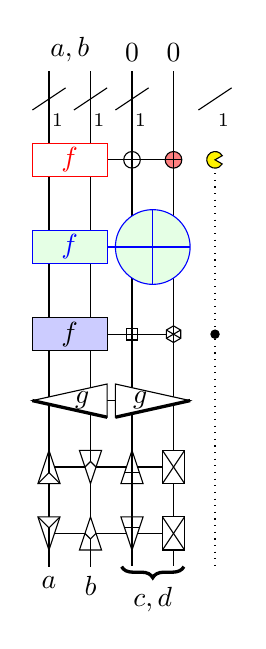
\begin{tikzpicture}[scale=1.000000,x=1pt,y=1pt]
\filldraw[color=white] (7.500000, 0.000000) rectangle (-67.500000, -179.000000);
% Drawing wires
% Line 2: a b W a,b
\draw[color=black] (-60.000000,0.000000) -- (-60.000000,-179.000000);
%   Deferring wire label at (-60.000000,0.000000)
% Line 5: x W owire
\draw[color=black,dotted] (-0.000000,-32.000000) -- (-0.000000,-179.000000);
% Line 3: c W 0
\draw[color=black] (-30.000000,0.000000) -- (-30.000000,-179.000000);
\draw[color=black] (-30.000000,0.000000) node[above] {$0$};
% Line 2: a b W a,b
\draw[color=black] (-45.000000,0.000000) -- (-45.000000,-179.000000);
\draw[color=black] (-52.500000,0.000000) node[above] {$a,b$};
% Line 4: d W 0
\draw[color=black] (-15.000000,0.000000) -- (-15.000000,-179.000000);
\draw[color=black] (-15.000000,0.000000) node[above] {$0$};
% Done with wires; drawing gates
% Line 11: a b c x / 1
\draw (-66.000000, -14.000000) -- (-54.000000, -6.000000);
\draw (-57.000000, -12.000000) node[below] {$\scriptstyle{1}$};
\draw (-51.000000, -14.000000) -- (-39.000000, -6.000000);
\draw (-42.000000, -12.000000) node[below] {$\scriptstyle{1}$};
\draw (-36.000000, -14.000000) -- (-24.000000, -6.000000);
\draw (-27.000000, -12.000000) node[below] {$\scriptstyle{1}$};
\draw (-6.000000, -14.000000) -- (6.000000, -6.000000);
\draw (3.000000, -12.000000) node[below] {$\scriptstyle{1}$};
% Line 12: x:op="\draw[fill=yellow] (0,0) -- (30:3pt) arc (30:330:3pt) -- cycle;":sh=0:style=dotted:qwire
\begin{scope}
\begin{scope}[shift={(-0.000000,-32.000000)}]
\draw[fill=yellow] (0,0) -- (30:3pt) arc (30:330:3pt) -- cycle;
\end{scope}
\end{scope}
% Line 13: a b G:color=red $f$ +c +d:fill=red!50!white
\draw (-60.000000,-32.000000) -- (-15.000000,-32.000000);
\begin{scope}[color=red]
\begin{scope}
\draw[fill=white] (-52.500000, -32.000000) +(-45.000000:19.091883pt and 8.485281pt) -- +(45.000000:19.091883pt and 8.485281pt) -- +(135.000000:19.091883pt and 8.485281pt) -- +(225.000000:19.091883pt and 8.485281pt) -- cycle;
\clip (-52.500000, -32.000000) +(-45.000000:19.091883pt and 8.485281pt) -- +(45.000000:19.091883pt and 8.485281pt) -- +(135.000000:19.091883pt and 8.485281pt) -- +(225.000000:19.091883pt and 8.485281pt) -- cycle;
\draw (-52.500000, -32.000000) node {$f$};
\end{scope}
\end{scope}
\begin{scope}
\draw[fill=white] (-30.000000, -32.000000) circle(3.000000pt);
\clip (-30.000000, -32.000000) circle(3.000000pt);
\draw (-33.000000, -32.000000) -- (-27.000000, -32.000000);
\draw (-30.000000, -35.000000) -- (-30.000000, -29.000000);
\end{scope}
\begin{scope}
\draw[fill=red!50!white] (-15.000000, -32.000000) circle(3.000000pt);
\clip (-15.000000, -32.000000) circle(3.000000pt);
\draw (-18.000000, -32.000000) -- (-12.000000, -32.000000);
\draw (-15.000000, -35.000000) -- (-15.000000, -29.000000);
\end{scope}
% Line 14: a b G $f$ c d P:size=27 + color=blue fi=green!10!white
\begin{scope}[color=blue]
\draw (-60.000000,-63.500000) -- (-15.000000,-63.500000);
\begin{scope}[color=blue]
\begin{scope}
\draw[fill=green!10!white] (-52.500000, -63.500000) +(-45.000000:19.091883pt and 8.485281pt) -- +(45.000000:19.091883pt and 8.485281pt) -- +(135.000000:19.091883pt and 8.485281pt) -- +(225.000000:19.091883pt and 8.485281pt) -- cycle;
\clip (-52.500000, -63.500000) +(-45.000000:19.091883pt and 8.485281pt) -- +(45.000000:19.091883pt and 8.485281pt) -- +(135.000000:19.091883pt and 8.485281pt) -- +(225.000000:19.091883pt and 8.485281pt) -- cycle;
\draw (-52.500000, -63.500000) node {$f$};
\end{scope}
\end{scope}
\begin{scope}[color=blue]
\begin{scope}
\draw[fill=green!10!white] (-22.500000, -63.500000) circle(13.500000pt);
\clip (-22.500000, -63.500000) circle(13.500000pt);
\draw (-36.000000, -63.500000) -- (-9.000000, -63.500000);
\draw (-22.500000, -77.000000) -- (-22.500000, -50.000000);
\end{scope}
\end{scope}
\end{scope}
% Line 15: x TOUCH
% Line 16: a b G:op=$f$ +c:sh=box d:sh=6:op=* fi=blue!20!white
\draw (-60.000000,-95.000000) -- (-15.000000,-95.000000);
\begin{scope}
\draw[fill=blue!20!white] (-52.500000, -95.000000) +(-45.000000:19.091883pt and 8.485281pt) -- +(45.000000:19.091883pt and 8.485281pt) -- +(135.000000:19.091883pt and 8.485281pt) -- +(225.000000:19.091883pt and 8.485281pt) -- cycle;
\clip (-52.500000, -95.000000) +(-45.000000:19.091883pt and 8.485281pt) -- +(45.000000:19.091883pt and 8.485281pt) -- +(135.000000:19.091883pt and 8.485281pt) -- +(225.000000:19.091883pt and 8.485281pt) -- cycle;
\draw (-52.500000, -95.000000) node {$f$};
\end{scope}
\begin{scope}
\draw[fill=white] (-30.000000, -95.000000) +(-45.000000:3.000000pt) -- +(45.000000:3.000000pt) -- +(135.000000:3.000000pt) -- +(225.000000:3.000000pt) -- cycle;
\clip (-30.000000, -95.000000) +(-45.000000:3.000000pt) -- +(45.000000:3.000000pt) -- +(135.000000:3.000000pt) -- +(225.000000:3.000000pt) -- cycle;
\draw (-33.000000, -95.000000) -- (-27.000000, -95.000000);
\draw (-30.000000, -98.000000) -- (-30.000000, -92.000000);
\end{scope}
\begin{scope}
\draw[fill=white] (-15.000000, -95.000000) +(-90.000000:3.000000pt) -- +(-30.000000:3.000000pt) -- +(30.000000:3.000000pt) -- +(90.000000:3.000000pt) -- +(150.000000:3.000000pt) -- +(210.000000:3.000000pt) -- cycle;
\clip (-15.000000, -95.000000) +(-90.000000:3.000000pt) -- +(-30.000000:3.000000pt) -- +(30.000000:3.000000pt) -- +(90.000000:3.000000pt) -- +(150.000000:3.000000pt) -- +(210.000000:3.000000pt) -- cycle;
\draw (-15.000000, -95.000000) -- +(-90.000000:3.000000pt);
\draw (-15.000000, -95.000000) -- +(-30.000000:3.000000pt);
\draw (-15.000000, -95.000000) -- +(30.000000:3.000000pt);
\draw (-15.000000, -95.000000) -- +(90.000000:3.000000pt);
\draw (-15.000000, -95.000000) -- +(150.000000:3.000000pt);
\draw (-15.000000, -95.000000) -- +(210.000000:3.000000pt);
\end{scope}
% Line 18: x:sh=1
\filldraw (-0.000000, -95.000000) circle(1.500000pt);
% Line 17: a b G|:shape=3 $g$ c d G|:shape=-3 $g$
\draw (-60.000000,-119.000000) -- (-15.000000,-119.000000);
\begin{scope}
\draw[fill=white] (-48.000000, -119.000000) +(-60.000000:18.000000pt and 6.928203pt) -- +(60.000000:18.000000pt and 6.928203pt) -- +(180.000000:18.000000pt and 6.928203pt) -- cycle;
\draw[very thick,solid] (-48.000000, -119.000000) +(180.000000:18.000000pt and 6.928203pt) -- +(-60.000000:18.000000pt and 6.928203pt);
\clip (-48.000000, -119.000000) +(-60.000000:18.000000pt and 6.928203pt) -- +(60.000000:18.000000pt and 6.928203pt) -- +(180.000000:18.000000pt and 6.928203pt) -- cycle;
\draw (-48.000000, -119.000000) node {$g$};
\end{scope}
\begin{scope}
\draw[fill=white] (-27.000000, -119.000000) +(0.000000:18.000000pt and 6.928203pt) -- +(120.000000:18.000000pt and 6.928203pt) -- +(240.000000:18.000000pt and 6.928203pt) -- cycle;
\draw[very thick,solid] (-27.000000, -119.000000) +(240.000000:18.000000pt and 6.928203pt) -- +(0.000000:18.000000pt and 6.928203pt);
\clip (-27.000000, -119.000000) +(0.000000:18.000000pt and 6.928203pt) -- +(120.000000:18.000000pt and 6.928203pt) -- +(240.000000:18.000000pt and 6.928203pt) -- cycle;
\draw (-27.000000, -119.000000) node {$g$};
\end{scope}
% Line 19: a G:op=*:sh=> b G:op=-*:sh=< c G:op=+:sh=> d G:op=x breadth=8
\draw (-60.000000,-143.000000) -- (-15.000000,-143.000000);
\begin{scope}
\draw[fill=white] (-60.000000, -145.000000) +(-30.000000:4.618802pt and 8.000000pt) -- +(90.000000:4.618802pt and 8.000000pt) -- +(210.000000:4.618802pt and 8.000000pt) -- cycle;
\clip (-60.000000, -145.000000) +(-30.000000:4.618802pt and 8.000000pt) -- +(90.000000:4.618802pt and 8.000000pt) -- +(210.000000:4.618802pt and 8.000000pt) -- cycle;
\draw (-60.000000, -145.000000) -- +(-30.000000:4.618802pt and 8.000000pt);
\draw (-60.000000, -145.000000) -- +(90.000000:4.618802pt and 8.000000pt);
\draw (-60.000000, -145.000000) -- +(210.000000:4.618802pt and 8.000000pt);
\end{scope}
\begin{scope}
\draw[fill=white] (-45.000000, -141.000000) +(-90.000000:4.618802pt and 8.000000pt) -- +(30.000000:4.618802pt and 8.000000pt) -- +(150.000000:4.618802pt and 8.000000pt) -- cycle;
\clip (-45.000000, -141.000000) +(-90.000000:4.618802pt and 8.000000pt) -- +(30.000000:4.618802pt and 8.000000pt) -- +(150.000000:4.618802pt and 8.000000pt) -- cycle;
\draw (-45.000000, -141.000000) -- +(-30.000000:4.618802pt and 8.000000pt);
\draw (-45.000000, -141.000000) -- +(90.000000:4.618802pt and 8.000000pt);
\draw (-45.000000, -141.000000) -- +(210.000000:4.618802pt and 8.000000pt);
\end{scope}
\begin{scope}
\draw[fill=white] (-30.000000, -145.000000) +(-30.000000:4.618802pt and 8.000000pt) -- +(90.000000:4.618802pt and 8.000000pt) -- +(210.000000:4.618802pt and 8.000000pt) -- cycle;
\clip (-30.000000, -145.000000) +(-30.000000:4.618802pt and 8.000000pt) -- +(90.000000:4.618802pt and 8.000000pt) -- +(210.000000:4.618802pt and 8.000000pt) -- cycle;
\draw (-34.618802, -145.000000) -- (-25.381198, -145.000000);
\draw (-30.000000, -153.000000) -- (-30.000000, -137.000000);
\end{scope}
\begin{scope}
\draw[fill=white] (-15.000000, -143.000000) +(-45.000000:5.656854pt and 8.485281pt) -- +(45.000000:5.656854pt and 8.485281pt) -- +(135.000000:5.656854pt and 8.485281pt) -- +(225.000000:5.656854pt and 8.485281pt) -- cycle;
\clip (-15.000000, -143.000000) +(-45.000000:5.656854pt and 8.485281pt) -- +(45.000000:5.656854pt and 8.485281pt) -- +(135.000000:5.656854pt and 8.485281pt) -- +(225.000000:5.656854pt and 8.485281pt) -- cycle;
\draw (-19.000000, -149.000000) -- (-11.000000, -137.000000);
\draw (-19.000000, -137.000000) -- (-11.000000, -149.000000);
\end{scope}
\draw (-60.000000,-167.000000) -- (-15.000000,-167.000000);
\begin{scope}
\draw[fill=white] (-60.000000, -165.000000) +(-90.000000:4.618802pt and 8.000000pt) -- +(30.000000:4.618802pt and 8.000000pt) -- +(150.000000:4.618802pt and 8.000000pt) -- cycle;
\clip (-60.000000, -165.000000) +(-90.000000:4.618802pt and 8.000000pt) -- +(30.000000:4.618802pt and 8.000000pt) -- +(150.000000:4.618802pt and 8.000000pt) -- cycle;
\draw (-60.000000, -165.000000) -- +(-90.000000:4.618802pt and 8.000000pt);
\draw (-60.000000, -165.000000) -- +(30.000000:4.618802pt and 8.000000pt);
\draw (-60.000000, -165.000000) -- +(150.000000:4.618802pt and 8.000000pt);
\end{scope}
\begin{scope}
\draw[fill=white] (-45.000000, -169.000000) +(-30.000000:4.618802pt and 8.000000pt) -- +(90.000000:4.618802pt and 8.000000pt) -- +(210.000000:4.618802pt and 8.000000pt) -- cycle;
\clip (-45.000000, -169.000000) +(-30.000000:4.618802pt and 8.000000pt) -- +(90.000000:4.618802pt and 8.000000pt) -- +(210.000000:4.618802pt and 8.000000pt) -- cycle;
\draw (-45.000000, -169.000000) -- +(30.000000:4.618802pt and 8.000000pt);
\draw (-45.000000, -169.000000) -- +(150.000000:4.618802pt and 8.000000pt);
\draw (-45.000000, -169.000000) -- +(270.000000:4.618802pt and 8.000000pt);
\end{scope}
\begin{scope}
\draw[fill=white] (-30.000000, -165.000000) +(-90.000000:4.618802pt and 8.000000pt) -- +(30.000000:4.618802pt and 8.000000pt) -- +(150.000000:4.618802pt and 8.000000pt) -- cycle;
\clip (-30.000000, -165.000000) +(-90.000000:4.618802pt and 8.000000pt) -- +(30.000000:4.618802pt and 8.000000pt) -- +(150.000000:4.618802pt and 8.000000pt) -- cycle;
\draw (-34.618802, -165.000000) -- (-25.381198, -165.000000);
\draw (-30.000000, -173.000000) -- (-30.000000, -157.000000);
\end{scope}
\begin{scope}
\draw[fill=white] (-15.000000, -167.000000) +(-45.000000:5.656854pt and 8.485281pt) -- +(45.000000:5.656854pt and 8.485281pt) -- +(135.000000:5.656854pt and 8.485281pt) -- +(225.000000:5.656854pt and 8.485281pt) -- cycle;
\clip (-15.000000, -167.000000) +(-45.000000:5.656854pt and 8.485281pt) -- +(45.000000:5.656854pt and 8.485281pt) -- +(135.000000:5.656854pt and 8.485281pt) -- +(225.000000:5.656854pt and 8.485281pt) -- cycle;
\draw (-19.000000, -173.000000) -- (-11.000000, -161.000000);
\draw (-19.000000, -161.000000) -- (-11.000000, -173.000000);
\end{scope}
% Done with gates; drawing ending labels
\draw[color=black] (-60.000000,-179.000000) node[below] {$a$};
%   Deferring wire label at (-30.000000,-179.000000)
\draw[color=black] (-45.000000,-179.000000) node[below] {$b$};
\filldraw[color=white,fill=white] (-11.250000,-179.000000) rectangle (-33.750000,-183.000000);
\draw[decorate,decoration={brace,amplitude = 4.000000pt},very thick] (-11.250000,-179.000000) -- (-33.750000,-179.000000);
\draw[color=black] (-22.500000,-183.000000) node[below] {$c,d$};
% Done with ending labels; drawing cut lines and comments
% Done with comments
\end{tikzpicture}

\end{figure}

\SaveVerb{name}|ShorNutshell|
\begin{figure}[ht]
\caption{\protect\UseVerb{name}}
\newcommand{\ket}[1]{\left| #1 \right\rangle}
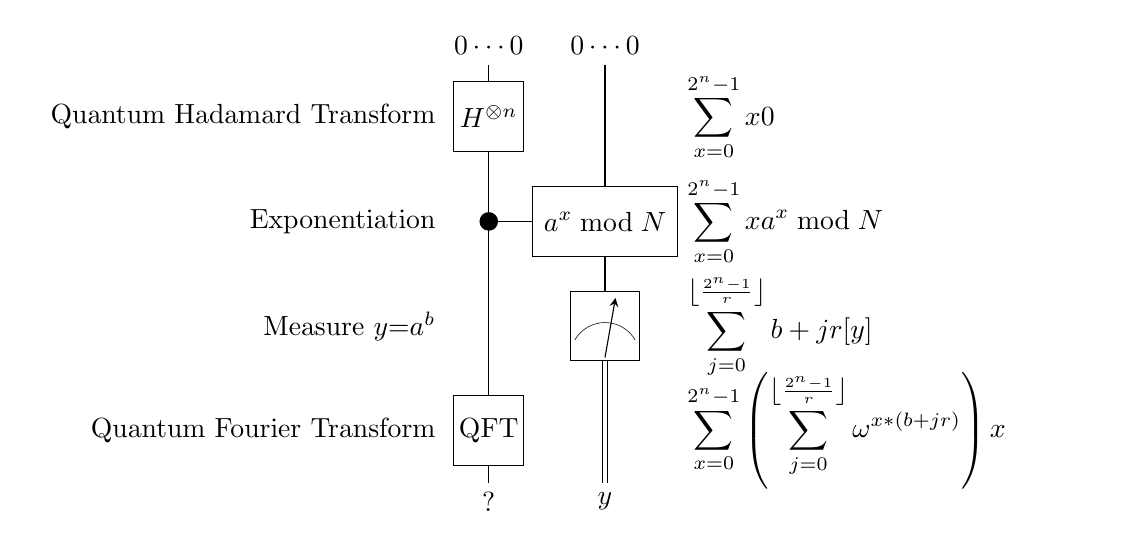
\begin{tikzpicture}[scale=2.100000,x=1pt,y=1pt]
\filldraw[color=white] (12.500000, 0.000000) rectangle (-27.500000, -72.000000);
% Drawing wires
% Line 7: x W \ket{0\cdots{}0} ?
\draw[color=black] (-20.000000,0.000000) -- (-20.000000,-72.000000);
\draw[color=black] (-20.000000,0.000000) node[above] {$\ket{0\cdots{}0}$};
% Line 8: y W \ket{0\cdots{}0} y width=25
\draw[color=black] (-0.000000,0.000000) -- (-0.000000,-45.000000);
\draw[color=black] (0.500000,-45.000000) -- (0.500000,-72.000000);
\draw[color=black] (-0.500000,-45.000000) -- (-0.500000,-72.000000);
\draw[color=black] (-0.000000,0.000000) node[above] {$\ket{0\cdots{}0}$};
% Done with wires; drawing gates
% Line 15: x G $H^{{\otimes}n}$ %Quantum Hadamard Transform% $\displaystyle\sum_{x=0}^{2^n-1}\ket{x}\ket{0}$
\draw (-27.500000, -9.000000) node[text width=144pt,left,text ragged left] {Quantum Hadamard Transform};
\draw (12.500000, -9.000000) node[text width=144pt,right] {$\displaystyle\sum_{x=0}^{2^n-1}\ket{x}\ket{0}$};
\begin{scope}
\draw[fill=white] (-20.000000, -9.000000) +(-45.000000:8.485281pt and 8.485281pt) -- +(45.000000:8.485281pt and 8.485281pt) -- +(135.000000:8.485281pt and 8.485281pt) -- +(225.000000:8.485281pt and 8.485281pt) -- cycle;
\clip (-20.000000, -9.000000) +(-45.000000:8.485281pt and 8.485281pt) -- +(45.000000:8.485281pt and 8.485281pt) -- +(135.000000:8.485281pt and 8.485281pt) -- +(225.000000:8.485281pt and 8.485281pt) -- cycle;
\draw (-20.000000, -9.000000) node {$H^{{\otimes}n}$};
\end{scope}
% Line 17: y G $a^x\bmod{}N$ x width=25 % Exponentiation% $\displaystyle\sum_{x=0}^{2^n-1}\ket{x}\ket{a^x\bmod{}N}$
\draw (-27.500000, -27.000000) node[text width=144pt,left,text ragged left] {Exponentiation};
\draw (12.500000, -27.000000) node[text width=144pt,right] {$\displaystyle\sum_{x=0}^{2^n-1}\ket{x}\ket{a^x\bmod{}N}$};
\draw (-20.000000,-27.000000) -- (-0.000000,-27.000000);
\begin{scope}
\draw[fill=white] (0.000000, -27.000000) +(-45.000000:17.677670pt and 8.485281pt) -- +(45.000000:17.677670pt and 8.485281pt) -- +(135.000000:17.677670pt and 8.485281pt) -- +(225.000000:17.677670pt and 8.485281pt) -- cycle;
\clip (0.000000, -27.000000) +(-45.000000:17.677670pt and 8.485281pt) -- +(45.000000:17.677670pt and 8.485281pt) -- +(135.000000:17.677670pt and 8.485281pt) -- +(225.000000:17.677670pt and 8.485281pt) -- cycle;
\draw (0.000000, -27.000000) node {$a^x\bmod{}N$};
\end{scope}
\filldraw (-20.000000, -27.000000) circle(1.500000pt);
% Line 19: y M % Measure $y{=}a^b$% $\displaystyle\sum_{j=0}^{\left\lfloor\frac{2^n-1}{r}\right\rfloor}\ket{b+jr}[y]$
\draw (-27.500000, -45.000000) node[text width=144pt,left,text ragged left] {Measure $y{=}a^b$};
\draw (12.500000, -45.000000) node[text width=144pt,right] {$\displaystyle\sum_{j=0}^{\left\lfloor\frac{2^n-1}{r}\right\rfloor}\ket{b+jr}[y]$};
\draw[fill=white] (-6.000000, -51.000000) rectangle (6.000000, -39.000000);
\draw[very thin] (-0.000000, -44.400000) arc (90:150:6.000000pt);
\draw[very thin] (-0.000000, -44.400000) arc (90:30:6.000000pt);
\draw[->,>=stealth] (-0.000000, -50.400000) -- +(80:10.392305pt);
% Line 21: x G QFT %Quantum Fourier Transform% $\displaystyle\sum_{x=0}^{2^n-1}\left(\sum_{j=0}^{\left\lfloor\frac{2^n-1}{r}\right\rfloor}\omega^{x*(b+jr)}\right)\ket{x}$
\draw (-27.500000, -63.000000) node[text width=144pt,left,text ragged left] {Quantum Fourier Transform};
\draw (12.500000, -63.000000) node[text width=144pt,right] {$\displaystyle\sum_{x=0}^{2^n-1}\left(\sum_{j=0}^{\left\lfloor\frac{2^n-1}{r}\right\rfloor}\omega^{x*(b+jr)}\right)\ket{x}$};
\begin{scope}
\draw[fill=white] (-20.000000, -63.000000) +(-45.000000:8.485281pt and 8.485281pt) -- +(45.000000:8.485281pt and 8.485281pt) -- +(135.000000:8.485281pt and 8.485281pt) -- +(225.000000:8.485281pt and 8.485281pt) -- cycle;
\clip (-20.000000, -63.000000) +(-45.000000:8.485281pt and 8.485281pt) -- +(45.000000:8.485281pt and 8.485281pt) -- +(135.000000:8.485281pt and 8.485281pt) -- +(225.000000:8.485281pt and 8.485281pt) -- cycle;
\draw (-20.000000, -63.000000) node {QFT};
\end{scope}
% Done with gates; drawing ending labels
\draw[color=black] (-20.000000,-72.000000) node[below] {$?$};
\draw[color=black] (-0.000000,-72.000000) node[below] {$y$};
% Done with ending labels; drawing cut lines and comments
% Done with comments
\end{tikzpicture}

\end{figure}

\SaveVerb{name}|Simon|
\begin{figure}[ht]
\caption{\protect\UseVerb{name}}
\providecommand{\ket}[1]{{\left\vert{#1}\right\rangle}}
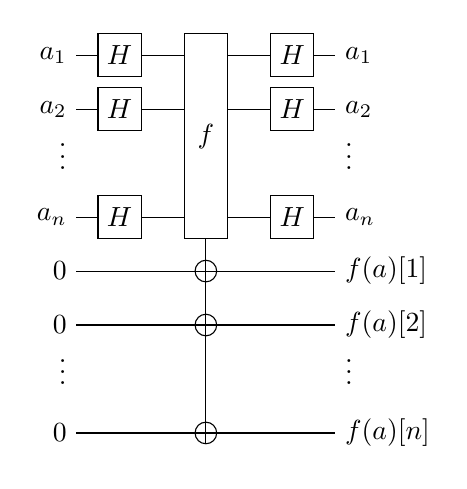
\begin{tikzpicture}[scale=1.300000,x=1pt,y=1pt]
\filldraw[color=white] (0.000000, -7.500000) rectangle (72.000000, 112.500000);
% Drawing wires
% Line 4: a1 W \ket{a_1} \ket{a_1}
\draw[color=black] (0.000000,105.000000) -- (72.000000,105.000000);
\draw[color=black] (0.000000,105.000000) node[left] {$\ket{a_1}$};
% Line 5: a2 W \ket{a_2} \ket{a_2}
\draw[color=black] (0.000000,90.000000) -- (72.000000,90.000000);
\draw[color=black] (0.000000,90.000000) node[left] {$\ket{a_2}$};
% Line 6: ...1 W
\draw[color=black] (0.000000,75.000000) node[anchor=mid east] {$\vdots$};
% Line 7: an W \ket{a_n} \ket{a_n}
\draw[color=black] (0.000000,60.000000) -- (72.000000,60.000000);
\draw[color=black] (0.000000,60.000000) node[left] {$\ket{a_n}$};
% Line 8: z1 W \ket{0} \ket{f(a)[1]}
\draw[color=black] (0.000000,45.000000) -- (72.000000,45.000000);
\draw[color=black] (0.000000,45.000000) node[left] {$\ket{0}$};
% Line 9: z2 W \ket{0} \ket{f(a)[2]}
\draw[color=black] (0.000000,30.000000) -- (72.000000,30.000000);
\draw[color=black] (0.000000,30.000000) node[left] {$\ket{0}$};
% Line 10: ...2 W
\draw[color=black] (0.000000,15.000000) node[anchor=mid east] {$\vdots$};
% Line 11: zn W \ket{0} \ket{f(a)[n]}
\draw[color=black] (0.000000,0.000000) -- (72.000000,0.000000);
\draw[color=black] (0.000000,0.000000) node[left] {$\ket{0}$};
% Done with wires; drawing gates
% Line 13: a1 H
\begin{scope}
\draw[fill=white] (12.000000, 105.000000) +(-45.000000:8.485281pt and 8.485281pt) -- +(45.000000:8.485281pt and 8.485281pt) -- +(135.000000:8.485281pt and 8.485281pt) -- +(225.000000:8.485281pt and 8.485281pt) -- cycle;
\clip (12.000000, 105.000000) +(-45.000000:8.485281pt and 8.485281pt) -- +(45.000000:8.485281pt and 8.485281pt) -- +(135.000000:8.485281pt and 8.485281pt) -- +(225.000000:8.485281pt and 8.485281pt) -- cycle;
\draw (12.000000, 105.000000) node {$H$};
\end{scope}
% Line 14: a2 H
\begin{scope}
\draw[fill=white] (12.000000, 90.000000) +(-45.000000:8.485281pt and 8.485281pt) -- +(45.000000:8.485281pt and 8.485281pt) -- +(135.000000:8.485281pt and 8.485281pt) -- +(225.000000:8.485281pt and 8.485281pt) -- cycle;
\clip (12.000000, 90.000000) +(-45.000000:8.485281pt and 8.485281pt) -- +(45.000000:8.485281pt and 8.485281pt) -- +(135.000000:8.485281pt and 8.485281pt) -- +(225.000000:8.485281pt and 8.485281pt) -- cycle;
\draw (12.000000, 90.000000) node {$H$};
\end{scope}
% Line 15: an H
\begin{scope}
\draw[fill=white] (12.000000, 60.000000) +(-45.000000:8.485281pt and 8.485281pt) -- +(45.000000:8.485281pt and 8.485281pt) -- +(135.000000:8.485281pt and 8.485281pt) -- +(225.000000:8.485281pt and 8.485281pt) -- cycle;
\clip (12.000000, 60.000000) +(-45.000000:8.485281pt and 8.485281pt) -- +(45.000000:8.485281pt and 8.485281pt) -- +(135.000000:8.485281pt and 8.485281pt) -- +(225.000000:8.485281pt and 8.485281pt) -- cycle;
\draw (12.000000, 60.000000) node {$H$};
\end{scope}
% Line 16: a1 a2 an G $f$ +z1 +z2 +zn
\draw (36.000000,105.000000) -- (36.000000,0.000000);
\begin{scope}
\draw[fill=white] (36.000000, 82.500000) +(-45.000000:8.485281pt and 40.305087pt) -- +(45.000000:8.485281pt and 40.305087pt) -- +(135.000000:8.485281pt and 40.305087pt) -- +(225.000000:8.485281pt and 40.305087pt) -- cycle;
\clip (36.000000, 82.500000) +(-45.000000:8.485281pt and 40.305087pt) -- +(45.000000:8.485281pt and 40.305087pt) -- +(135.000000:8.485281pt and 40.305087pt) -- +(225.000000:8.485281pt and 40.305087pt) -- cycle;
\draw (36.000000, 82.500000) node {$f$};
\end{scope}
\begin{scope}
\draw[fill=white] (36.000000, 45.000000) circle(3.000000pt);
\clip (36.000000, 45.000000) circle(3.000000pt);
\draw (33.000000, 45.000000) -- (39.000000, 45.000000);
\draw (36.000000, 42.000000) -- (36.000000, 48.000000);
\end{scope}
\begin{scope}
\draw[fill=white] (36.000000, 30.000000) circle(3.000000pt);
\clip (36.000000, 30.000000) circle(3.000000pt);
\draw (33.000000, 30.000000) -- (39.000000, 30.000000);
\draw (36.000000, 27.000000) -- (36.000000, 33.000000);
\end{scope}
\begin{scope}
\draw[fill=white] (36.000000, 0.000000) circle(3.000000pt);
\clip (36.000000, 0.000000) circle(3.000000pt);
\draw (33.000000, 0.000000) -- (39.000000, 0.000000);
\draw (36.000000, -3.000000) -- (36.000000, 3.000000);
\end{scope}
% Line 17: a1 H
\begin{scope}
\draw[fill=white] (60.000000, 105.000000) +(-45.000000:8.485281pt and 8.485281pt) -- +(45.000000:8.485281pt and 8.485281pt) -- +(135.000000:8.485281pt and 8.485281pt) -- +(225.000000:8.485281pt and 8.485281pt) -- cycle;
\clip (60.000000, 105.000000) +(-45.000000:8.485281pt and 8.485281pt) -- +(45.000000:8.485281pt and 8.485281pt) -- +(135.000000:8.485281pt and 8.485281pt) -- +(225.000000:8.485281pt and 8.485281pt) -- cycle;
\draw (60.000000, 105.000000) node {$H$};
\end{scope}
% Line 18: a2 H
\begin{scope}
\draw[fill=white] (60.000000, 90.000000) +(-45.000000:8.485281pt and 8.485281pt) -- +(45.000000:8.485281pt and 8.485281pt) -- +(135.000000:8.485281pt and 8.485281pt) -- +(225.000000:8.485281pt and 8.485281pt) -- cycle;
\clip (60.000000, 90.000000) +(-45.000000:8.485281pt and 8.485281pt) -- +(45.000000:8.485281pt and 8.485281pt) -- +(135.000000:8.485281pt and 8.485281pt) -- +(225.000000:8.485281pt and 8.485281pt) -- cycle;
\draw (60.000000, 90.000000) node {$H$};
\end{scope}
% Line 19: an H
\begin{scope}
\draw[fill=white] (60.000000, 60.000000) +(-45.000000:8.485281pt and 8.485281pt) -- +(45.000000:8.485281pt and 8.485281pt) -- +(135.000000:8.485281pt and 8.485281pt) -- +(225.000000:8.485281pt and 8.485281pt) -- cycle;
\clip (60.000000, 60.000000) +(-45.000000:8.485281pt and 8.485281pt) -- +(45.000000:8.485281pt and 8.485281pt) -- +(135.000000:8.485281pt and 8.485281pt) -- +(225.000000:8.485281pt and 8.485281pt) -- cycle;
\draw (60.000000, 60.000000) node {$H$};
\end{scope}
% Done with gates; drawing ending labels
\draw[color=black] (72.000000,105.000000) node[right] {$\ket{a_1}$};
\draw[color=black] (72.000000,90.000000) node[right] {$\ket{a_2}$};
\draw[color=black] (72.000000,75.000000) node[anchor=mid west] {$\vdots$};
\draw[color=black] (72.000000,60.000000) node[right] {$\ket{a_n}$};
\draw[color=black] (72.000000,45.000000) node[right] {$\ket{f(a)[1]}$};
\draw[color=black] (72.000000,30.000000) node[right] {$\ket{f(a)[2]}$};
\draw[color=black] (72.000000,15.000000) node[anchor=mid west] {$\vdots$};
\draw[color=black] (72.000000,0.000000) node[right] {$\ket{f(a)[n]}$};
% Done with ending labels; drawing cut lines and comments
% Done with comments
\end{tikzpicture}

\end{figure}

\SaveVerb{name}|Steane_NOOP|
\begin{figure}[ht]
\caption{\protect\UseVerb{name}}
%! \usetikzlibrary{decorations.pathreplacing,decorations.pathmorphing}
\providecommand{\ket}[1]{{\left\vert{#1}\right\rangle}}
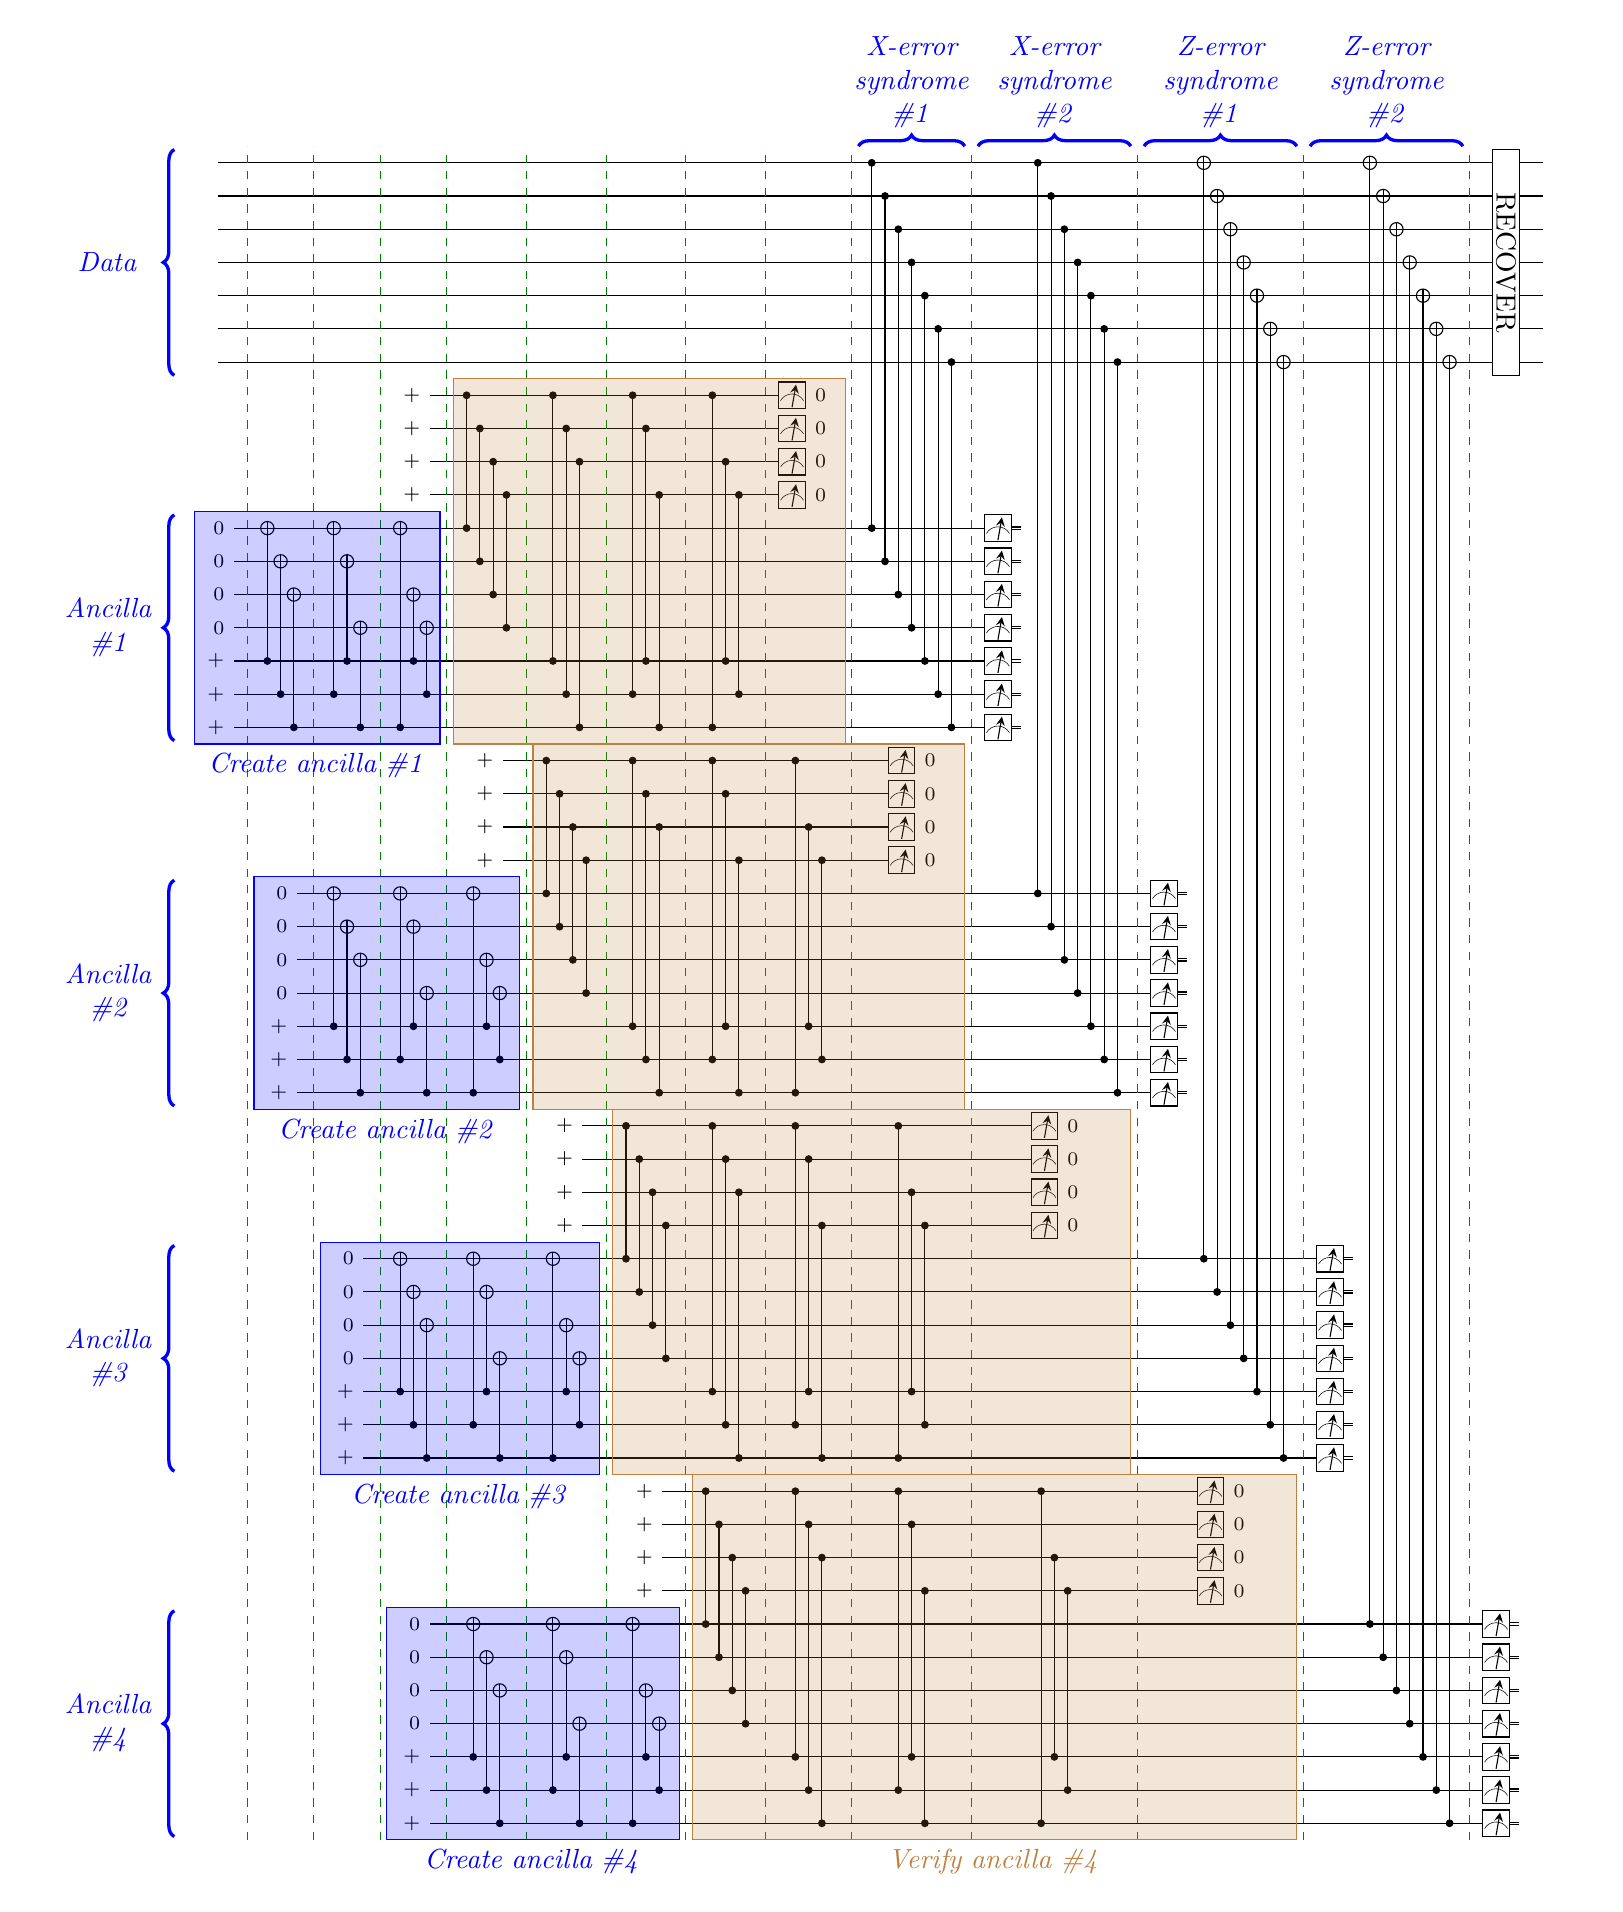
\begin{tikzpicture}[scale=0.800000,x=1pt,y=1pt]
\filldraw[color=white] (0.000000, -7.500000) rectangle (684.000000, 757.500000);
% Drawing wires
% Line 5: data0 W
\draw[color=black] (85.500000,750.000000) -- (684.000000,750.000000);
% Line 6: data1 W
\draw[color=black] (85.500000,735.000000) -- (684.000000,735.000000);
% Line 7: data2 W
\draw[color=black] (85.500000,720.000000) -- (684.000000,720.000000);
% Line 8: data3 W
\draw[color=black] (85.500000,705.000000) -- (684.000000,705.000000);
% Line 9: data4 W
\draw[color=black] (85.500000,690.000000) -- (684.000000,690.000000);
% Line 10: data5 W
\draw[color=black] (85.500000,675.000000) -- (684.000000,675.000000);
% Line 11: data6 W
\draw[color=black] (85.500000,660.000000) -- (684.000000,660.000000);
% Line 12: x00 W \ket{+} 0
\draw[color=black] (174.000000,645.000000) -- (345.000000,645.000000);
\draw[color=black] (345.000000,644.500000) -- (358.500000,644.500000);
\draw[color=black] (345.000000,645.500000) -- (358.500000,645.500000);
% Line 13: x01 W \ket{+} 0
\draw[color=black] (174.000000,630.000000) -- (345.000000,630.000000);
\draw[color=black] (345.000000,629.500000) -- (358.500000,629.500000);
\draw[color=black] (345.000000,630.500000) -- (358.500000,630.500000);
% Line 14: x02 W \ket{+} 0
\draw[color=black] (174.000000,615.000000) -- (345.000000,615.000000);
\draw[color=black] (345.000000,614.500000) -- (358.500000,614.500000);
\draw[color=black] (345.000000,615.500000) -- (358.500000,615.500000);
% Line 15: x03 W \ket{+} 0
\draw[color=black] (174.000000,600.000000) -- (345.000000,600.000000);
\draw[color=black] (345.000000,599.500000) -- (358.500000,599.500000);
\draw[color=black] (345.000000,600.500000) -- (358.500000,600.500000);
% Line 16: a00 W \ket{0}
\draw[color=black] (85.500000,585.000000) -- (438.000000,585.000000);
\draw[color=black] (438.000000,584.500000) -- (448.500000,584.500000);
\draw[color=black] (438.000000,585.500000) -- (448.500000,585.500000);
% Line 17: a01 W \ket{0}
\draw[color=black] (85.500000,570.000000) -- (438.000000,570.000000);
\draw[color=black] (438.000000,569.500000) -- (448.500000,569.500000);
\draw[color=black] (438.000000,570.500000) -- (448.500000,570.500000);
% Line 18: a02 W \ket{0}
\draw[color=black] (85.500000,555.000000) -- (438.000000,555.000000);
\draw[color=black] (438.000000,554.500000) -- (448.500000,554.500000);
\draw[color=black] (438.000000,555.500000) -- (448.500000,555.500000);
% Line 19: a03 W \ket{0}
\draw[color=black] (85.500000,540.000000) -- (438.000000,540.000000);
\draw[color=black] (438.000000,539.500000) -- (448.500000,539.500000);
\draw[color=black] (438.000000,540.500000) -- (448.500000,540.500000);
% Line 20: a04 W \ket{+}
\draw[color=black] (85.500000,525.000000) -- (438.000000,525.000000);
\draw[color=black] (438.000000,524.500000) -- (448.500000,524.500000);
\draw[color=black] (438.000000,525.500000) -- (448.500000,525.500000);
% Line 21: a05 W \ket{+}
\draw[color=black] (85.500000,510.000000) -- (438.000000,510.000000);
\draw[color=black] (438.000000,509.500000) -- (448.500000,509.500000);
\draw[color=black] (438.000000,510.500000) -- (448.500000,510.500000);
% Line 22: a06 W \ket{+}
\draw[color=black] (85.500000,495.000000) -- (438.000000,495.000000);
\draw[color=black] (438.000000,494.500000) -- (448.500000,494.500000);
\draw[color=black] (438.000000,495.500000) -- (448.500000,495.500000);
% Line 23: x10 W \ket{+} 0
\draw[color=black] (207.000000,480.000000) -- (394.500000,480.000000);
\draw[color=black] (394.500000,479.500000) -- (405.000000,479.500000);
\draw[color=black] (394.500000,480.500000) -- (405.000000,480.500000);
% Line 24: x11 W \ket{+} 0
\draw[color=black] (207.000000,465.000000) -- (394.500000,465.000000);
\draw[color=black] (394.500000,464.500000) -- (405.000000,464.500000);
\draw[color=black] (394.500000,465.500000) -- (405.000000,465.500000);
% Line 25: x12 W \ket{+} 0
\draw[color=black] (207.000000,450.000000) -- (394.500000,450.000000);
\draw[color=black] (394.500000,449.500000) -- (405.000000,449.500000);
\draw[color=black] (394.500000,450.500000) -- (405.000000,450.500000);
% Line 26: x13 W \ket{+} 0
\draw[color=black] (207.000000,435.000000) -- (394.500000,435.000000);
\draw[color=black] (394.500000,434.500000) -- (405.000000,434.500000);
\draw[color=black] (394.500000,435.500000) -- (405.000000,435.500000);
% Line 27: a10 W \ket{0}
\draw[color=black] (114.000000,420.000000) -- (513.000000,420.000000);
\draw[color=black] (513.000000,419.500000) -- (523.500000,419.500000);
\draw[color=black] (513.000000,420.500000) -- (523.500000,420.500000);
% Line 28: a11 W \ket{0}
\draw[color=black] (114.000000,405.000000) -- (513.000000,405.000000);
\draw[color=black] (513.000000,404.500000) -- (523.500000,404.500000);
\draw[color=black] (513.000000,405.500000) -- (523.500000,405.500000);
% Line 29: a12 W \ket{0}
\draw[color=black] (114.000000,390.000000) -- (513.000000,390.000000);
\draw[color=black] (513.000000,389.500000) -- (523.500000,389.500000);
\draw[color=black] (513.000000,390.500000) -- (523.500000,390.500000);
% Line 30: a13 W \ket{0}
\draw[color=black] (114.000000,375.000000) -- (513.000000,375.000000);
\draw[color=black] (513.000000,374.500000) -- (523.500000,374.500000);
\draw[color=black] (513.000000,375.500000) -- (523.500000,375.500000);
% Line 31: a14 W \ket{+}
\draw[color=black] (114.000000,360.000000) -- (513.000000,360.000000);
\draw[color=black] (513.000000,359.500000) -- (523.500000,359.500000);
\draw[color=black] (513.000000,360.500000) -- (523.500000,360.500000);
% Line 32: a15 W \ket{+}
\draw[color=black] (114.000000,345.000000) -- (513.000000,345.000000);
\draw[color=black] (513.000000,344.500000) -- (523.500000,344.500000);
\draw[color=black] (513.000000,345.500000) -- (523.500000,345.500000);
% Line 33: a16 W \ket{+}
\draw[color=black] (114.000000,330.000000) -- (513.000000,330.000000);
\draw[color=black] (513.000000,329.500000) -- (523.500000,329.500000);
\draw[color=black] (513.000000,330.500000) -- (523.500000,330.500000);
% Line 34: x20 W \ket{+} 0
\draw[color=black] (243.000000,315.000000) -- (459.000000,315.000000);
\draw[color=black] (459.000000,314.500000) -- (469.500000,314.500000);
\draw[color=black] (459.000000,315.500000) -- (469.500000,315.500000);
% Line 35: x21 W \ket{+} 0
\draw[color=black] (243.000000,300.000000) -- (459.000000,300.000000);
\draw[color=black] (459.000000,299.500000) -- (469.500000,299.500000);
\draw[color=black] (459.000000,300.500000) -- (469.500000,300.500000);
% Line 36: x22 W \ket{+} 0
\draw[color=black] (243.000000,285.000000) -- (459.000000,285.000000);
\draw[color=black] (459.000000,284.500000) -- (469.500000,284.500000);
\draw[color=black] (459.000000,285.500000) -- (469.500000,285.500000);
% Line 37: x23 W \ket{+} 0
\draw[color=black] (243.000000,270.000000) -- (459.000000,270.000000);
\draw[color=black] (459.000000,269.500000) -- (469.500000,269.500000);
\draw[color=black] (459.000000,270.500000) -- (469.500000,270.500000);
% Line 38: a20 W \ket{0}
\draw[color=black] (144.000000,255.000000) -- (588.000000,255.000000);
\draw[color=black] (588.000000,254.500000) -- (598.500000,254.500000);
\draw[color=black] (588.000000,255.500000) -- (598.500000,255.500000);
% Line 39: a21 W \ket{0}
\draw[color=black] (144.000000,240.000000) -- (588.000000,240.000000);
\draw[color=black] (588.000000,239.500000) -- (598.500000,239.500000);
\draw[color=black] (588.000000,240.500000) -- (598.500000,240.500000);
% Line 40: a22 W \ket{0}
\draw[color=black] (144.000000,225.000000) -- (588.000000,225.000000);
\draw[color=black] (588.000000,224.500000) -- (598.500000,224.500000);
\draw[color=black] (588.000000,225.500000) -- (598.500000,225.500000);
% Line 41: a23 W \ket{0}
\draw[color=black] (144.000000,210.000000) -- (588.000000,210.000000);
\draw[color=black] (588.000000,209.500000) -- (598.500000,209.500000);
\draw[color=black] (588.000000,210.500000) -- (598.500000,210.500000);
% Line 42: a24 W \ket{+}
\draw[color=black] (144.000000,195.000000) -- (588.000000,195.000000);
\draw[color=black] (588.000000,194.500000) -- (598.500000,194.500000);
\draw[color=black] (588.000000,195.500000) -- (598.500000,195.500000);
% Line 43: a25 W \ket{+}
\draw[color=black] (144.000000,180.000000) -- (588.000000,180.000000);
\draw[color=black] (588.000000,179.500000) -- (598.500000,179.500000);
\draw[color=black] (588.000000,180.500000) -- (598.500000,180.500000);
% Line 44: a26 W \ket{+}
\draw[color=black] (144.000000,165.000000) -- (588.000000,165.000000);
\draw[color=black] (588.000000,164.500000) -- (598.500000,164.500000);
\draw[color=black] (588.000000,165.500000) -- (598.500000,165.500000);
% Line 45: x30 W \ket{+} 0
\draw[color=black] (279.000000,150.000000) -- (534.000000,150.000000);
\draw[color=black] (534.000000,149.500000) -- (544.500000,149.500000);
\draw[color=black] (534.000000,150.500000) -- (544.500000,150.500000);
% Line 46: x31 W \ket{+} 0
\draw[color=black] (279.000000,135.000000) -- (534.000000,135.000000);
\draw[color=black] (534.000000,134.500000) -- (544.500000,134.500000);
\draw[color=black] (534.000000,135.500000) -- (544.500000,135.500000);
% Line 47: x32 W \ket{+} 0
\draw[color=black] (279.000000,120.000000) -- (534.000000,120.000000);
\draw[color=black] (534.000000,119.500000) -- (544.500000,119.500000);
\draw[color=black] (534.000000,120.500000) -- (544.500000,120.500000);
% Line 48: x33 W \ket{+} 0
\draw[color=black] (279.000000,105.000000) -- (534.000000,105.000000);
\draw[color=black] (534.000000,104.500000) -- (544.500000,104.500000);
\draw[color=black] (534.000000,105.500000) -- (544.500000,105.500000);
% Line 49: a30 W \ket{0}
\draw[color=black] (174.000000,90.000000) -- (663.000000,90.000000);
\draw[color=black] (663.000000,89.500000) -- (673.500000,89.500000);
\draw[color=black] (663.000000,90.500000) -- (673.500000,90.500000);
% Line 50: a31 W \ket{0}
\draw[color=black] (174.000000,75.000000) -- (663.000000,75.000000);
\draw[color=black] (663.000000,74.500000) -- (673.500000,74.500000);
\draw[color=black] (663.000000,75.500000) -- (673.500000,75.500000);
% Line 51: a32 W \ket{0}
\draw[color=black] (174.000000,60.000000) -- (663.000000,60.000000);
\draw[color=black] (663.000000,59.500000) -- (673.500000,59.500000);
\draw[color=black] (663.000000,60.500000) -- (673.500000,60.500000);
% Line 52: a33 W \ket{0}
\draw[color=black] (174.000000,45.000000) -- (663.000000,45.000000);
\draw[color=black] (663.000000,44.500000) -- (673.500000,44.500000);
\draw[color=black] (663.000000,45.500000) -- (673.500000,45.500000);
% Line 53: a34 W \ket{+}
\draw[color=black] (174.000000,30.000000) -- (663.000000,30.000000);
\draw[color=black] (663.000000,29.500000) -- (673.500000,29.500000);
\draw[color=black] (663.000000,30.500000) -- (673.500000,30.500000);
% Line 54: a35 W \ket{+}
\draw[color=black] (174.000000,15.000000) -- (663.000000,15.000000);
\draw[color=black] (663.000000,14.500000) -- (673.500000,14.500000);
\draw[color=black] (663.000000,15.500000) -- (673.500000,15.500000);
% Line 55: a36 W \ket{+}
\draw[color=black] (174.000000,0.000000) -- (663.000000,0.000000);
\draw[color=black] (663.000000,-0.500000) -- (673.500000,-0.500000);
\draw[color=black] (663.000000,0.500000) -- (673.500000,0.500000);
% Done with wires; drawing gates
% Line 60: data0 data6 =< color=blue \emph{Data} length=60
\begin{scope}[color=blue]
\draw[fill=white,color=white] (6.000000, 654.000000) rectangle (66.000000, 756.000000);
\draw (36.000000, 705.000000) node {\emph{Data}};
\draw[decorate,decoration={brace,amplitude = 4.000000pt},very thick] (66.000000,654.000000) -- (66.000000,756.000000);
\end{scope}
% Line 61: a00 a01 a02 a03 a04 a05 a06 =< color=blue length=60 \emph{\begin{tabular}{c}Ancilla \\ \#1\end{tabular}}
\begin{scope}[color=blue]
\draw[fill=white,color=white] (6.000000, 489.000000) rectangle (66.000000, 591.000000);
\draw (36.000000, 540.000000) node {\emph{\begin{tabular}{c}Ancilla \\ \#1\end{tabular}}};
\draw[decorate,decoration={brace,amplitude = 4.000000pt},very thick] (66.000000,489.000000) -- (66.000000,591.000000);
\end{scope}
% Line 62: a10 a11 a12 a13 a14 a15 a16 =< color=blue length=60 \emph{\begin{tabular}{c}Ancilla \\ \#2\end{tabular}}
\begin{scope}[color=blue]
\draw[fill=white,color=white] (6.000000, 324.000000) rectangle (66.000000, 426.000000);
\draw (36.000000, 375.000000) node {\emph{\begin{tabular}{c}Ancilla \\ \#2\end{tabular}}};
\draw[decorate,decoration={brace,amplitude = 4.000000pt},very thick] (66.000000,324.000000) -- (66.000000,426.000000);
\end{scope}
% Line 63: a20 a21 a22 a23 a24 a25 a26 =< color=blue length=60 \emph{\begin{tabular}{c}Ancilla \\ \#3\end{tabular}}
\begin{scope}[color=blue]
\draw[fill=white,color=white] (6.000000, 159.000000) rectangle (66.000000, 261.000000);
\draw (36.000000, 210.000000) node {\emph{\begin{tabular}{c}Ancilla \\ \#3\end{tabular}}};
\draw[decorate,decoration={brace,amplitude = 4.000000pt},very thick] (66.000000,159.000000) -- (66.000000,261.000000);
\end{scope}
% Line 64: a30 a31 a32 a33 a34 a35 a36 =< color=blue length=60 \emph{\begin{tabular}{c}Ancilla \\ \#4\end{tabular}}
\begin{scope}[color=blue]
\draw[fill=white,color=white] (6.000000, -6.000000) rectangle (66.000000, 96.000000);
\draw (36.000000, 45.000000) node {\emph{\begin{tabular}{c}Ancilla \\ \#4\end{tabular}}};
\draw[decorate,decoration={brace,amplitude = 4.000000pt},very thick] (66.000000,-6.000000) -- (66.000000,96.000000);
\end{scope}
% Line 66: a00 a01 a02 a03 a04 a05 a06 data0 data1 data2 data3 data4 data5 data6 START
\draw[color=black] (93.000000,585.000000) node[fill=white,left,minimum height=15.000000pt,minimum width=15.000000pt,inner sep=0pt] {\phantom{$\scriptstyle\ket{0}$}};
\draw[color=black] (93.000000,585.000000) node[left] {$\scriptstyle\ket{0}$};
\draw[color=black] (93.000000,570.000000) node[fill=white,left,minimum height=15.000000pt,minimum width=15.000000pt,inner sep=0pt] {\phantom{$\scriptstyle\ket{0}$}};
\draw[color=black] (93.000000,570.000000) node[left] {$\scriptstyle\ket{0}$};
\draw[color=black] (93.000000,555.000000) node[fill=white,left,minimum height=15.000000pt,minimum width=15.000000pt,inner sep=0pt] {\phantom{$\scriptstyle\ket{0}$}};
\draw[color=black] (93.000000,555.000000) node[left] {$\scriptstyle\ket{0}$};
\draw[color=black] (93.000000,540.000000) node[fill=white,left,minimum height=15.000000pt,minimum width=15.000000pt,inner sep=0pt] {\phantom{$\scriptstyle\ket{0}$}};
\draw[color=black] (93.000000,540.000000) node[left] {$\scriptstyle\ket{0}$};
\draw[color=black] (93.000000,525.000000) node[fill=white,left,minimum height=15.000000pt,minimum width=15.000000pt,inner sep=0pt] {\phantom{$\scriptstyle\ket{+}$}};
\draw[color=black] (93.000000,525.000000) node[left] {$\scriptstyle\ket{+}$};
\draw[color=black] (93.000000,510.000000) node[fill=white,left,minimum height=15.000000pt,minimum width=15.000000pt,inner sep=0pt] {\phantom{$\scriptstyle\ket{+}$}};
\draw[color=black] (93.000000,510.000000) node[left] {$\scriptstyle\ket{+}$};
\draw[color=black] (93.000000,495.000000) node[fill=white,left,minimum height=15.000000pt,minimum width=15.000000pt,inner sep=0pt] {\phantom{$\scriptstyle\ket{+}$}};
\draw[color=black] (93.000000,495.000000) node[left] {$\scriptstyle\ket{+}$};
% Line 68: +a00 a04
\draw (108.000000,585.000000) -- (108.000000,525.000000);
\begin{scope}
\draw[fill=white] (108.000000, 585.000000) circle(3.000000pt);
\clip (108.000000, 585.000000) circle(3.000000pt);
\draw (105.000000, 585.000000) -- (111.000000, 585.000000);
\draw (108.000000, 582.000000) -- (108.000000, 588.000000);
\end{scope}
\filldraw (108.000000, 525.000000) circle(1.500000pt);
% Line 69: +a01 a05
\draw (114.000000,570.000000) -- (114.000000,510.000000);
\begin{scope}
\draw[fill=white] (114.000000, 570.000000) circle(3.000000pt);
\clip (114.000000, 570.000000) circle(3.000000pt);
\draw (111.000000, 570.000000) -- (117.000000, 570.000000);
\draw (114.000000, 567.000000) -- (114.000000, 573.000000);
\end{scope}
\filldraw (114.000000, 510.000000) circle(1.500000pt);
% Line 70: +a02 a06
\draw (120.000000,555.000000) -- (120.000000,495.000000);
\begin{scope}
\draw[fill=white] (120.000000, 555.000000) circle(3.000000pt);
\clip (120.000000, 555.000000) circle(3.000000pt);
\draw (117.000000, 555.000000) -- (123.000000, 555.000000);
\draw (120.000000, 552.000000) -- (120.000000, 558.000000);
\end{scope}
\filldraw (120.000000, 495.000000) circle(1.500000pt);
% Line 71: a10 a11 a12 a13 a14 a15 a16 START
\draw[color=black] (121.500000,420.000000) node[fill=white,left,minimum height=15.000000pt,minimum width=15.000000pt,inner sep=0pt] {\phantom{$\scriptstyle\ket{0}$}};
\draw[color=black] (121.500000,420.000000) node[left] {$\scriptstyle\ket{0}$};
\draw[color=black] (121.500000,405.000000) node[fill=white,left,minimum height=15.000000pt,minimum width=15.000000pt,inner sep=0pt] {\phantom{$\scriptstyle\ket{0}$}};
\draw[color=black] (121.500000,405.000000) node[left] {$\scriptstyle\ket{0}$};
\draw[color=black] (121.500000,390.000000) node[fill=white,left,minimum height=15.000000pt,minimum width=15.000000pt,inner sep=0pt] {\phantom{$\scriptstyle\ket{0}$}};
\draw[color=black] (121.500000,390.000000) node[left] {$\scriptstyle\ket{0}$};
\draw[color=black] (121.500000,375.000000) node[fill=white,left,minimum height=15.000000pt,minimum width=15.000000pt,inner sep=0pt] {\phantom{$\scriptstyle\ket{0}$}};
\draw[color=black] (121.500000,375.000000) node[left] {$\scriptstyle\ket{0}$};
\draw[color=black] (121.500000,360.000000) node[fill=white,left,minimum height=15.000000pt,minimum width=15.000000pt,inner sep=0pt] {\phantom{$\scriptstyle\ket{+}$}};
\draw[color=black] (121.500000,360.000000) node[left] {$\scriptstyle\ket{+}$};
\draw[color=black] (121.500000,345.000000) node[fill=white,left,minimum height=15.000000pt,minimum width=15.000000pt,inner sep=0pt] {\phantom{$\scriptstyle\ket{+}$}};
\draw[color=black] (121.500000,345.000000) node[left] {$\scriptstyle\ket{+}$};
\draw[color=black] (121.500000,330.000000) node[fill=white,left,minimum height=15.000000pt,minimum width=15.000000pt,inner sep=0pt] {\phantom{$\scriptstyle\ket{+}$}};
\draw[color=black] (121.500000,330.000000) node[left] {$\scriptstyle\ket{+}$};
% Line 73: +a00 a05
\draw (138.000000,585.000000) -- (138.000000,510.000000);
\begin{scope}
\draw[fill=white] (138.000000, 585.000000) circle(3.000000pt);
\clip (138.000000, 585.000000) circle(3.000000pt);
\draw (135.000000, 585.000000) -- (141.000000, 585.000000);
\draw (138.000000, 582.000000) -- (138.000000, 588.000000);
\end{scope}
\filldraw (138.000000, 510.000000) circle(1.500000pt);
% Line 74: +a01 a04
\draw (144.000000,570.000000) -- (144.000000,525.000000);
\begin{scope}
\draw[fill=white] (144.000000, 570.000000) circle(3.000000pt);
\clip (144.000000, 570.000000) circle(3.000000pt);
\draw (141.000000, 570.000000) -- (147.000000, 570.000000);
\draw (144.000000, 567.000000) -- (144.000000, 573.000000);
\end{scope}
\filldraw (144.000000, 525.000000) circle(1.500000pt);
% Line 75: +a03 a06
\draw (150.000000,540.000000) -- (150.000000,495.000000);
\begin{scope}
\draw[fill=white] (150.000000, 540.000000) circle(3.000000pt);
\clip (150.000000, 540.000000) circle(3.000000pt);
\draw (147.000000, 540.000000) -- (153.000000, 540.000000);
\draw (150.000000, 537.000000) -- (150.000000, 543.000000);
\end{scope}
\filldraw (150.000000, 495.000000) circle(1.500000pt);
% Line 76: +a10 a14
\draw (138.000000,420.000000) -- (138.000000,360.000000);
\begin{scope}
\draw[fill=white] (138.000000, 420.000000) circle(3.000000pt);
\clip (138.000000, 420.000000) circle(3.000000pt);
\draw (135.000000, 420.000000) -- (141.000000, 420.000000);
\draw (138.000000, 417.000000) -- (138.000000, 423.000000);
\end{scope}
\filldraw (138.000000, 360.000000) circle(1.500000pt);
% Line 77: +a11 a15
\draw (144.000000,405.000000) -- (144.000000,345.000000);
\begin{scope}
\draw[fill=white] (144.000000, 405.000000) circle(3.000000pt);
\clip (144.000000, 405.000000) circle(3.000000pt);
\draw (141.000000, 405.000000) -- (147.000000, 405.000000);
\draw (144.000000, 402.000000) -- (144.000000, 408.000000);
\end{scope}
\filldraw (144.000000, 345.000000) circle(1.500000pt);
% Line 78: +a12 a16
\draw (150.000000,390.000000) -- (150.000000,330.000000);
\begin{scope}
\draw[fill=white] (150.000000, 390.000000) circle(3.000000pt);
\clip (150.000000, 390.000000) circle(3.000000pt);
\draw (147.000000, 390.000000) -- (153.000000, 390.000000);
\draw (150.000000, 387.000000) -- (150.000000, 393.000000);
\end{scope}
\filldraw (150.000000, 330.000000) circle(1.500000pt);
% Line 79: a20 a21 a22 a23 a24 a25 a26 START
\draw[color=black] (151.500000,255.000000) node[fill=white,left,minimum height=15.000000pt,minimum width=15.000000pt,inner sep=0pt] {\phantom{$\scriptstyle\ket{0}$}};
\draw[color=black] (151.500000,255.000000) node[left] {$\scriptstyle\ket{0}$};
\draw[color=black] (151.500000,240.000000) node[fill=white,left,minimum height=15.000000pt,minimum width=15.000000pt,inner sep=0pt] {\phantom{$\scriptstyle\ket{0}$}};
\draw[color=black] (151.500000,240.000000) node[left] {$\scriptstyle\ket{0}$};
\draw[color=black] (151.500000,225.000000) node[fill=white,left,minimum height=15.000000pt,minimum width=15.000000pt,inner sep=0pt] {\phantom{$\scriptstyle\ket{0}$}};
\draw[color=black] (151.500000,225.000000) node[left] {$\scriptstyle\ket{0}$};
\draw[color=black] (151.500000,210.000000) node[fill=white,left,minimum height=15.000000pt,minimum width=15.000000pt,inner sep=0pt] {\phantom{$\scriptstyle\ket{0}$}};
\draw[color=black] (151.500000,210.000000) node[left] {$\scriptstyle\ket{0}$};
\draw[color=black] (151.500000,195.000000) node[fill=white,left,minimum height=15.000000pt,minimum width=15.000000pt,inner sep=0pt] {\phantom{$\scriptstyle\ket{+}$}};
\draw[color=black] (151.500000,195.000000) node[left] {$\scriptstyle\ket{+}$};
\draw[color=black] (151.500000,180.000000) node[fill=white,left,minimum height=15.000000pt,minimum width=15.000000pt,inner sep=0pt] {\phantom{$\scriptstyle\ket{+}$}};
\draw[color=black] (151.500000,180.000000) node[left] {$\scriptstyle\ket{+}$};
\draw[color=black] (151.500000,165.000000) node[fill=white,left,minimum height=15.000000pt,minimum width=15.000000pt,inner sep=0pt] {\phantom{$\scriptstyle\ket{+}$}};
\draw[color=black] (151.500000,165.000000) node[left] {$\scriptstyle\ket{+}$};
% Line 81: +a00 a06
\draw (168.000000,585.000000) -- (168.000000,495.000000);
\begin{scope}
\draw[fill=white] (168.000000, 585.000000) circle(3.000000pt);
\clip (168.000000, 585.000000) circle(3.000000pt);
\draw (165.000000, 585.000000) -- (171.000000, 585.000000);
\draw (168.000000, 582.000000) -- (168.000000, 588.000000);
\end{scope}
\filldraw (168.000000, 495.000000) circle(1.500000pt);
% Line 82: +a02 a04
\draw (174.000000,555.000000) -- (174.000000,525.000000);
\begin{scope}
\draw[fill=white] (174.000000, 555.000000) circle(3.000000pt);
\clip (174.000000, 555.000000) circle(3.000000pt);
\draw (171.000000, 555.000000) -- (177.000000, 555.000000);
\draw (174.000000, 552.000000) -- (174.000000, 558.000000);
\end{scope}
\filldraw (174.000000, 525.000000) circle(1.500000pt);
% Line 83: +a03 a05
\draw (180.000000,540.000000) -- (180.000000,510.000000);
\begin{scope}
\draw[fill=white] (180.000000, 540.000000) circle(3.000000pt);
\clip (180.000000, 540.000000) circle(3.000000pt);
\draw (177.000000, 540.000000) -- (183.000000, 540.000000);
\draw (180.000000, 537.000000) -- (180.000000, 543.000000);
\end{scope}
\filldraw (180.000000, 510.000000) circle(1.500000pt);
% Line 84: +a10 a15
\draw (168.000000,420.000000) -- (168.000000,345.000000);
\begin{scope}
\draw[fill=white] (168.000000, 420.000000) circle(3.000000pt);
\clip (168.000000, 420.000000) circle(3.000000pt);
\draw (165.000000, 420.000000) -- (171.000000, 420.000000);
\draw (168.000000, 417.000000) -- (168.000000, 423.000000);
\end{scope}
\filldraw (168.000000, 345.000000) circle(1.500000pt);
% Line 85: +a11 a14
\draw (174.000000,405.000000) -- (174.000000,360.000000);
\begin{scope}
\draw[fill=white] (174.000000, 405.000000) circle(3.000000pt);
\clip (174.000000, 405.000000) circle(3.000000pt);
\draw (171.000000, 405.000000) -- (177.000000, 405.000000);
\draw (174.000000, 402.000000) -- (174.000000, 408.000000);
\end{scope}
\filldraw (174.000000, 360.000000) circle(1.500000pt);
% Line 86: +a13 a16
\draw (180.000000,375.000000) -- (180.000000,330.000000);
\begin{scope}
\draw[fill=white] (180.000000, 375.000000) circle(3.000000pt);
\clip (180.000000, 375.000000) circle(3.000000pt);
\draw (177.000000, 375.000000) -- (183.000000, 375.000000);
\draw (180.000000, 372.000000) -- (180.000000, 378.000000);
\end{scope}
\filldraw (180.000000, 330.000000) circle(1.500000pt);
% Line 87: +a20 a24
\draw (168.000000,255.000000) -- (168.000000,195.000000);
\begin{scope}
\draw[fill=white] (168.000000, 255.000000) circle(3.000000pt);
\clip (168.000000, 255.000000) circle(3.000000pt);
\draw (165.000000, 255.000000) -- (171.000000, 255.000000);
\draw (168.000000, 252.000000) -- (168.000000, 258.000000);
\end{scope}
\filldraw (168.000000, 195.000000) circle(1.500000pt);
% Line 88: +a21 a25
\draw (174.000000,240.000000) -- (174.000000,180.000000);
\begin{scope}
\draw[fill=white] (174.000000, 240.000000) circle(3.000000pt);
\clip (174.000000, 240.000000) circle(3.000000pt);
\draw (171.000000, 240.000000) -- (177.000000, 240.000000);
\draw (174.000000, 237.000000) -- (174.000000, 243.000000);
\end{scope}
\filldraw (174.000000, 180.000000) circle(1.500000pt);
% Line 89: +a22 a26
\draw (180.000000,225.000000) -- (180.000000,165.000000);
\begin{scope}
\draw[fill=white] (180.000000, 225.000000) circle(3.000000pt);
\clip (180.000000, 225.000000) circle(3.000000pt);
\draw (177.000000, 225.000000) -- (183.000000, 225.000000);
\draw (180.000000, 222.000000) -- (180.000000, 228.000000);
\end{scope}
\filldraw (180.000000, 165.000000) circle(1.500000pt);
% Line 90: a30 a31 a32 a33 a34 a35 a36 START
\draw[color=black] (181.500000,90.000000) node[fill=white,left,minimum height=15.000000pt,minimum width=15.000000pt,inner sep=0pt] {\phantom{$\scriptstyle\ket{0}$}};
\draw[color=black] (181.500000,90.000000) node[left] {$\scriptstyle\ket{0}$};
\draw[color=black] (181.500000,75.000000) node[fill=white,left,minimum height=15.000000pt,minimum width=15.000000pt,inner sep=0pt] {\phantom{$\scriptstyle\ket{0}$}};
\draw[color=black] (181.500000,75.000000) node[left] {$\scriptstyle\ket{0}$};
\draw[color=black] (181.500000,60.000000) node[fill=white,left,minimum height=15.000000pt,minimum width=15.000000pt,inner sep=0pt] {\phantom{$\scriptstyle\ket{0}$}};
\draw[color=black] (181.500000,60.000000) node[left] {$\scriptstyle\ket{0}$};
\draw[color=black] (181.500000,45.000000) node[fill=white,left,minimum height=15.000000pt,minimum width=15.000000pt,inner sep=0pt] {\phantom{$\scriptstyle\ket{0}$}};
\draw[color=black] (181.500000,45.000000) node[left] {$\scriptstyle\ket{0}$};
\draw[color=black] (181.500000,30.000000) node[fill=white,left,minimum height=15.000000pt,minimum width=15.000000pt,inner sep=0pt] {\phantom{$\scriptstyle\ket{+}$}};
\draw[color=black] (181.500000,30.000000) node[left] {$\scriptstyle\ket{+}$};
\draw[color=black] (181.500000,15.000000) node[fill=white,left,minimum height=15.000000pt,minimum width=15.000000pt,inner sep=0pt] {\phantom{$\scriptstyle\ket{+}$}};
\draw[color=black] (181.500000,15.000000) node[left] {$\scriptstyle\ket{+}$};
\draw[color=black] (181.500000,0.000000) node[fill=white,left,minimum height=15.000000pt,minimum width=15.000000pt,inner sep=0pt] {\phantom{$\scriptstyle\ket{+}$}};
\draw[color=black] (181.500000,0.000000) node[left] {$\scriptstyle\ket{+}$};
% Line 91: x00 x01 x02 x03 START
\draw[color=black] (181.500000,645.000000) node[fill=white,left,minimum height=15.000000pt,minimum width=15.000000pt,inner sep=0pt] {\phantom{$\scriptstyle\ket{+}$}};
\draw[color=black] (181.500000,645.000000) node[left] {$\scriptstyle\ket{+}$};
\draw[color=black] (181.500000,630.000000) node[fill=white,left,minimum height=15.000000pt,minimum width=15.000000pt,inner sep=0pt] {\phantom{$\scriptstyle\ket{+}$}};
\draw[color=black] (181.500000,630.000000) node[left] {$\scriptstyle\ket{+}$};
\draw[color=black] (181.500000,615.000000) node[fill=white,left,minimum height=15.000000pt,minimum width=15.000000pt,inner sep=0pt] {\phantom{$\scriptstyle\ket{+}$}};
\draw[color=black] (181.500000,615.000000) node[left] {$\scriptstyle\ket{+}$};
\draw[color=black] (181.500000,600.000000) node[fill=white,left,minimum height=15.000000pt,minimum width=15.000000pt,inner sep=0pt] {\phantom{$\scriptstyle\ket{+}$}};
\draw[color=black] (181.500000,600.000000) node[left] {$\scriptstyle\ket{+}$};
% Line 93: +a10 a16
\draw (201.000000,420.000000) -- (201.000000,330.000000);
\begin{scope}
\draw[fill=white] (201.000000, 420.000000) circle(3.000000pt);
\clip (201.000000, 420.000000) circle(3.000000pt);
\draw (198.000000, 420.000000) -- (204.000000, 420.000000);
\draw (201.000000, 417.000000) -- (201.000000, 423.000000);
\end{scope}
\filldraw (201.000000, 330.000000) circle(1.500000pt);
% Line 94: +a12 a14
\draw (207.000000,390.000000) -- (207.000000,360.000000);
\begin{scope}
\draw[fill=white] (207.000000, 390.000000) circle(3.000000pt);
\clip (207.000000, 390.000000) circle(3.000000pt);
\draw (204.000000, 390.000000) -- (210.000000, 390.000000);
\draw (207.000000, 387.000000) -- (207.000000, 393.000000);
\end{scope}
\filldraw (207.000000, 360.000000) circle(1.500000pt);
% Line 95: +a13 a15
\draw (213.000000,375.000000) -- (213.000000,345.000000);
\begin{scope}
\draw[fill=white] (213.000000, 375.000000) circle(3.000000pt);
\clip (213.000000, 375.000000) circle(3.000000pt);
\draw (210.000000, 375.000000) -- (216.000000, 375.000000);
\draw (213.000000, 372.000000) -- (213.000000, 378.000000);
\end{scope}
\filldraw (213.000000, 345.000000) circle(1.500000pt);
% Line 96: +a20 a25
\draw (201.000000,255.000000) -- (201.000000,180.000000);
\begin{scope}
\draw[fill=white] (201.000000, 255.000000) circle(3.000000pt);
\clip (201.000000, 255.000000) circle(3.000000pt);
\draw (198.000000, 255.000000) -- (204.000000, 255.000000);
\draw (201.000000, 252.000000) -- (201.000000, 258.000000);
\end{scope}
\filldraw (201.000000, 180.000000) circle(1.500000pt);
% Line 97: +a21 a24
\draw (207.000000,240.000000) -- (207.000000,195.000000);
\begin{scope}
\draw[fill=white] (207.000000, 240.000000) circle(3.000000pt);
\clip (207.000000, 240.000000) circle(3.000000pt);
\draw (204.000000, 240.000000) -- (210.000000, 240.000000);
\draw (207.000000, 237.000000) -- (207.000000, 243.000000);
\end{scope}
\filldraw (207.000000, 195.000000) circle(1.500000pt);
% Line 98: +a23 a26
\draw (213.000000,210.000000) -- (213.000000,165.000000);
\begin{scope}
\draw[fill=white] (213.000000, 210.000000) circle(3.000000pt);
\clip (213.000000, 210.000000) circle(3.000000pt);
\draw (210.000000, 210.000000) -- (216.000000, 210.000000);
\draw (213.000000, 207.000000) -- (213.000000, 213.000000);
\end{scope}
\filldraw (213.000000, 165.000000) circle(1.500000pt);
% Line 99: +a30 a34
\draw (201.000000,90.000000) -- (201.000000,30.000000);
\begin{scope}
\draw[fill=white] (201.000000, 90.000000) circle(3.000000pt);
\clip (201.000000, 90.000000) circle(3.000000pt);
\draw (198.000000, 90.000000) -- (204.000000, 90.000000);
\draw (201.000000, 87.000000) -- (201.000000, 93.000000);
\end{scope}
\filldraw (201.000000, 30.000000) circle(1.500000pt);
% Line 100: +a31 a35
\draw (207.000000,75.000000) -- (207.000000,15.000000);
\begin{scope}
\draw[fill=white] (207.000000, 75.000000) circle(3.000000pt);
\clip (207.000000, 75.000000) circle(3.000000pt);
\draw (204.000000, 75.000000) -- (210.000000, 75.000000);
\draw (207.000000, 72.000000) -- (207.000000, 78.000000);
\end{scope}
\filldraw (207.000000, 15.000000) circle(1.500000pt);
% Line 101: +a32 a36
\draw (213.000000,60.000000) -- (213.000000,0.000000);
\begin{scope}
\draw[fill=white] (213.000000, 60.000000) circle(3.000000pt);
\clip (213.000000, 60.000000) circle(3.000000pt);
\draw (210.000000, 60.000000) -- (216.000000, 60.000000);
\draw (213.000000, 57.000000) -- (213.000000, 63.000000);
\end{scope}
\filldraw (213.000000, 0.000000) circle(1.500000pt);
% Line 102: a00 x00 #Z
\draw (198.000000,645.000000) -- (198.000000,585.000000);
\filldraw (198.000000, 585.000000) circle(1.500000pt);
\filldraw (198.000000, 645.000000) circle(1.500000pt);
% Line 103: a01 x01 #Z
\draw (204.000000,630.000000) -- (204.000000,570.000000);
\filldraw (204.000000, 570.000000) circle(1.500000pt);
\filldraw (204.000000, 630.000000) circle(1.500000pt);
% Line 104: a02 x02 #Z
\draw (210.000000,615.000000) -- (210.000000,555.000000);
\filldraw (210.000000, 555.000000) circle(1.500000pt);
\filldraw (210.000000, 615.000000) circle(1.500000pt);
% Line 105: a03 x03 #Z
\draw (216.000000,600.000000) -- (216.000000,540.000000);
\filldraw (216.000000, 540.000000) circle(1.500000pt);
\filldraw (216.000000, 600.000000) circle(1.500000pt);
% Line 106: x10 x11 x12 x13 START
\draw[color=black] (214.500000,480.000000) node[fill=white,left,minimum height=15.000000pt,minimum width=15.000000pt,inner sep=0pt] {\phantom{$\scriptstyle\ket{+}$}};
\draw[color=black] (214.500000,480.000000) node[left] {$\scriptstyle\ket{+}$};
\draw[color=black] (214.500000,465.000000) node[fill=white,left,minimum height=15.000000pt,minimum width=15.000000pt,inner sep=0pt] {\phantom{$\scriptstyle\ket{+}$}};
\draw[color=black] (214.500000,465.000000) node[left] {$\scriptstyle\ket{+}$};
\draw[color=black] (214.500000,450.000000) node[fill=white,left,minimum height=15.000000pt,minimum width=15.000000pt,inner sep=0pt] {\phantom{$\scriptstyle\ket{+}$}};
\draw[color=black] (214.500000,450.000000) node[left] {$\scriptstyle\ket{+}$};
\draw[color=black] (214.500000,435.000000) node[fill=white,left,minimum height=15.000000pt,minimum width=15.000000pt,inner sep=0pt] {\phantom{$\scriptstyle\ket{+}$}};
\draw[color=black] (214.500000,435.000000) node[left] {$\scriptstyle\ket{+}$};
% Line 108: +a20 a26
\draw (237.000000,255.000000) -- (237.000000,165.000000);
\begin{scope}
\draw[fill=white] (237.000000, 255.000000) circle(3.000000pt);
\clip (237.000000, 255.000000) circle(3.000000pt);
\draw (234.000000, 255.000000) -- (240.000000, 255.000000);
\draw (237.000000, 252.000000) -- (237.000000, 258.000000);
\end{scope}
\filldraw (237.000000, 165.000000) circle(1.500000pt);
% Line 109: +a22 a24
\draw (243.000000,225.000000) -- (243.000000,195.000000);
\begin{scope}
\draw[fill=white] (243.000000, 225.000000) circle(3.000000pt);
\clip (243.000000, 225.000000) circle(3.000000pt);
\draw (240.000000, 225.000000) -- (246.000000, 225.000000);
\draw (243.000000, 222.000000) -- (243.000000, 228.000000);
\end{scope}
\filldraw (243.000000, 195.000000) circle(1.500000pt);
% Line 110: +a23 a25
\draw (249.000000,210.000000) -- (249.000000,180.000000);
\begin{scope}
\draw[fill=white] (249.000000, 210.000000) circle(3.000000pt);
\clip (249.000000, 210.000000) circle(3.000000pt);
\draw (246.000000, 210.000000) -- (252.000000, 210.000000);
\draw (249.000000, 207.000000) -- (249.000000, 213.000000);
\end{scope}
\filldraw (249.000000, 180.000000) circle(1.500000pt);
% Line 111: +a30 a35
\draw (237.000000,90.000000) -- (237.000000,15.000000);
\begin{scope}
\draw[fill=white] (237.000000, 90.000000) circle(3.000000pt);
\clip (237.000000, 90.000000) circle(3.000000pt);
\draw (234.000000, 90.000000) -- (240.000000, 90.000000);
\draw (237.000000, 87.000000) -- (237.000000, 93.000000);
\end{scope}
\filldraw (237.000000, 15.000000) circle(1.500000pt);
% Line 112: +a31 a34
\draw (243.000000,75.000000) -- (243.000000,30.000000);
\begin{scope}
\draw[fill=white] (243.000000, 75.000000) circle(3.000000pt);
\clip (243.000000, 75.000000) circle(3.000000pt);
\draw (240.000000, 75.000000) -- (246.000000, 75.000000);
\draw (243.000000, 72.000000) -- (243.000000, 78.000000);
\end{scope}
\filldraw (243.000000, 30.000000) circle(1.500000pt);
% Line 113: +a33 a36
\draw (249.000000,45.000000) -- (249.000000,0.000000);
\begin{scope}
\draw[fill=white] (249.000000, 45.000000) circle(3.000000pt);
\clip (249.000000, 45.000000) circle(3.000000pt);
\draw (246.000000, 45.000000) -- (252.000000, 45.000000);
\draw (249.000000, 42.000000) -- (249.000000, 48.000000);
\end{scope}
\filldraw (249.000000, 0.000000) circle(1.500000pt);
% Line 114: a10 x10 #Z
\draw (234.000000,480.000000) -- (234.000000,420.000000);
\filldraw (234.000000, 420.000000) circle(1.500000pt);
\filldraw (234.000000, 480.000000) circle(1.500000pt);
% Line 115: a11 x11 #Z
\draw (240.000000,465.000000) -- (240.000000,405.000000);
\filldraw (240.000000, 405.000000) circle(1.500000pt);
\filldraw (240.000000, 465.000000) circle(1.500000pt);
% Line 116: a12 x12 #Z
\draw (246.000000,450.000000) -- (246.000000,390.000000);
\filldraw (246.000000, 390.000000) circle(1.500000pt);
\filldraw (246.000000, 450.000000) circle(1.500000pt);
% Line 117: a13 x13 #Z
\draw (252.000000,435.000000) -- (252.000000,375.000000);
\filldraw (252.000000, 375.000000) circle(1.500000pt);
\filldraw (252.000000, 435.000000) circle(1.500000pt);
% Line 118: a04 x00 #Z
\draw (237.000000,645.000000) -- (237.000000,525.000000);
\filldraw (237.000000, 525.000000) circle(1.500000pt);
\filldraw (237.000000, 645.000000) circle(1.500000pt);
% Line 119: a05 x01 #Z
\draw (243.000000,630.000000) -- (243.000000,510.000000);
\filldraw (243.000000, 510.000000) circle(1.500000pt);
\filldraw (243.000000, 630.000000) circle(1.500000pt);
% Line 120: a06 x02 #Z
\draw (249.000000,615.000000) -- (249.000000,495.000000);
\filldraw (249.000000, 495.000000) circle(1.500000pt);
\filldraw (249.000000, 615.000000) circle(1.500000pt);
% Line 121: x20 x21 x22 x23 START
\draw[color=black] (250.500000,315.000000) node[fill=white,left,minimum height=15.000000pt,minimum width=15.000000pt,inner sep=0pt] {\phantom{$\scriptstyle\ket{+}$}};
\draw[color=black] (250.500000,315.000000) node[left] {$\scriptstyle\ket{+}$};
\draw[color=black] (250.500000,300.000000) node[fill=white,left,minimum height=15.000000pt,minimum width=15.000000pt,inner sep=0pt] {\phantom{$\scriptstyle\ket{+}$}};
\draw[color=black] (250.500000,300.000000) node[left] {$\scriptstyle\ket{+}$};
\draw[color=black] (250.500000,285.000000) node[fill=white,left,minimum height=15.000000pt,minimum width=15.000000pt,inner sep=0pt] {\phantom{$\scriptstyle\ket{+}$}};
\draw[color=black] (250.500000,285.000000) node[left] {$\scriptstyle\ket{+}$};
\draw[color=black] (250.500000,270.000000) node[fill=white,left,minimum height=15.000000pt,minimum width=15.000000pt,inner sep=0pt] {\phantom{$\scriptstyle\ket{+}$}};
\draw[color=black] (250.500000,270.000000) node[left] {$\scriptstyle\ket{+}$};
% Line 123: +a30 a36
\draw (273.000000,90.000000) -- (273.000000,0.000000);
\begin{scope}
\draw[fill=white] (273.000000, 90.000000) circle(3.000000pt);
\clip (273.000000, 90.000000) circle(3.000000pt);
\draw (270.000000, 90.000000) -- (276.000000, 90.000000);
\draw (273.000000, 87.000000) -- (273.000000, 93.000000);
\end{scope}
\filldraw (273.000000, 0.000000) circle(1.500000pt);
% Line 124: +a32 a34
\draw (279.000000,60.000000) -- (279.000000,30.000000);
\begin{scope}
\draw[fill=white] (279.000000, 60.000000) circle(3.000000pt);
\clip (279.000000, 60.000000) circle(3.000000pt);
\draw (276.000000, 60.000000) -- (282.000000, 60.000000);
\draw (279.000000, 57.000000) -- (279.000000, 63.000000);
\end{scope}
\filldraw (279.000000, 30.000000) circle(1.500000pt);
% Line 125: +a33 a35
\draw (285.000000,45.000000) -- (285.000000,15.000000);
\begin{scope}
\draw[fill=white] (285.000000, 45.000000) circle(3.000000pt);
\clip (285.000000, 45.000000) circle(3.000000pt);
\draw (282.000000, 45.000000) -- (288.000000, 45.000000);
\draw (285.000000, 42.000000) -- (285.000000, 48.000000);
\end{scope}
\filldraw (285.000000, 15.000000) circle(1.500000pt);
% Line 126: a20 x20 #Z
\draw (270.000000,315.000000) -- (270.000000,255.000000);
\filldraw (270.000000, 255.000000) circle(1.500000pt);
\filldraw (270.000000, 315.000000) circle(1.500000pt);
% Line 127: a21 x21 #Z
\draw (276.000000,300.000000) -- (276.000000,240.000000);
\filldraw (276.000000, 240.000000) circle(1.500000pt);
\filldraw (276.000000, 300.000000) circle(1.500000pt);
% Line 128: a22 x22 #Z
\draw (282.000000,285.000000) -- (282.000000,225.000000);
\filldraw (282.000000, 225.000000) circle(1.500000pt);
\filldraw (282.000000, 285.000000) circle(1.500000pt);
% Line 129: a23 x23 #Z
\draw (288.000000,270.000000) -- (288.000000,210.000000);
\filldraw (288.000000, 210.000000) circle(1.500000pt);
\filldraw (288.000000, 270.000000) circle(1.500000pt);
% Line 130: a14 x10 #Z
\draw (273.000000,480.000000) -- (273.000000,360.000000);
\filldraw (273.000000, 360.000000) circle(1.500000pt);
\filldraw (273.000000, 480.000000) circle(1.500000pt);
% Line 131: a15 x11 #Z
\draw (279.000000,465.000000) -- (279.000000,345.000000);
\filldraw (279.000000, 345.000000) circle(1.500000pt);
\filldraw (279.000000, 465.000000) circle(1.500000pt);
% Line 132: a16 x12 #Z
\draw (285.000000,450.000000) -- (285.000000,330.000000);
\filldraw (285.000000, 330.000000) circle(1.500000pt);
\filldraw (285.000000, 450.000000) circle(1.500000pt);
% Line 133: a05 x00 #Z
\draw (273.000000,645.000000) -- (273.000000,510.000000);
\filldraw (273.000000, 510.000000) circle(1.500000pt);
\filldraw (273.000000, 645.000000) circle(1.500000pt);
% Line 134: a04 x01 #Z
\draw (279.000000,630.000000) -- (279.000000,525.000000);
\filldraw (279.000000, 525.000000) circle(1.500000pt);
\filldraw (279.000000, 630.000000) circle(1.500000pt);
% Line 135: a06 x03 #Z
\draw (285.000000,600.000000) -- (285.000000,495.000000);
\filldraw (285.000000, 495.000000) circle(1.500000pt);
\filldraw (285.000000, 600.000000) circle(1.500000pt);
% Line 136: x30 x31 x32 x33 START
\draw[color=black] (286.500000,150.000000) node[fill=white,left,minimum height=15.000000pt,minimum width=15.000000pt,inner sep=0pt] {\phantom{$\scriptstyle\ket{+}$}};
\draw[color=black] (286.500000,150.000000) node[left] {$\scriptstyle\ket{+}$};
\draw[color=black] (286.500000,135.000000) node[fill=white,left,minimum height=15.000000pt,minimum width=15.000000pt,inner sep=0pt] {\phantom{$\scriptstyle\ket{+}$}};
\draw[color=black] (286.500000,135.000000) node[left] {$\scriptstyle\ket{+}$};
\draw[color=black] (286.500000,120.000000) node[fill=white,left,minimum height=15.000000pt,minimum width=15.000000pt,inner sep=0pt] {\phantom{$\scriptstyle\ket{+}$}};
\draw[color=black] (286.500000,120.000000) node[left] {$\scriptstyle\ket{+}$};
\draw[color=black] (286.500000,105.000000) node[fill=white,left,minimum height=15.000000pt,minimum width=15.000000pt,inner sep=0pt] {\phantom{$\scriptstyle\ket{+}$}};
\draw[color=black] (286.500000,105.000000) node[left] {$\scriptstyle\ket{+}$};
% Line 138: a30 x30 #Z
\draw (306.000000,150.000000) -- (306.000000,90.000000);
\filldraw (306.000000, 90.000000) circle(1.500000pt);
\filldraw (306.000000, 150.000000) circle(1.500000pt);
% Line 139: a31 x31 #Z
\draw (312.000000,135.000000) -- (312.000000,75.000000);
\filldraw (312.000000, 75.000000) circle(1.500000pt);
\filldraw (312.000000, 135.000000) circle(1.500000pt);
% Line 140: a32 x32 #Z
\draw (318.000000,120.000000) -- (318.000000,60.000000);
\filldraw (318.000000, 60.000000) circle(1.500000pt);
\filldraw (318.000000, 120.000000) circle(1.500000pt);
% Line 141: a33 x33 #Z
\draw (324.000000,105.000000) -- (324.000000,45.000000);
\filldraw (324.000000, 45.000000) circle(1.500000pt);
\filldraw (324.000000, 105.000000) circle(1.500000pt);
% Line 142: a24 x20 #Z
\draw (309.000000,315.000000) -- (309.000000,195.000000);
\filldraw (309.000000, 195.000000) circle(1.500000pt);
\filldraw (309.000000, 315.000000) circle(1.500000pt);
% Line 143: a25 x21 #Z
\draw (315.000000,300.000000) -- (315.000000,180.000000);
\filldraw (315.000000, 180.000000) circle(1.500000pt);
\filldraw (315.000000, 300.000000) circle(1.500000pt);
% Line 144: a26 x22 #Z
\draw (321.000000,285.000000) -- (321.000000,165.000000);
\filldraw (321.000000, 165.000000) circle(1.500000pt);
\filldraw (321.000000, 285.000000) circle(1.500000pt);
% Line 145: a15 x10 #Z
\draw (309.000000,480.000000) -- (309.000000,345.000000);
\filldraw (309.000000, 345.000000) circle(1.500000pt);
\filldraw (309.000000, 480.000000) circle(1.500000pt);
% Line 146: a14 x11 #Z
\draw (315.000000,465.000000) -- (315.000000,360.000000);
\filldraw (315.000000, 360.000000) circle(1.500000pt);
\filldraw (315.000000, 465.000000) circle(1.500000pt);
% Line 147: a16 x13 #Z
\draw (321.000000,435.000000) -- (321.000000,330.000000);
\filldraw (321.000000, 330.000000) circle(1.500000pt);
\filldraw (321.000000, 435.000000) circle(1.500000pt);
% Line 148: a06 x00 #Z
\draw (309.000000,645.000000) -- (309.000000,495.000000);
\filldraw (309.000000, 495.000000) circle(1.500000pt);
\filldraw (309.000000, 645.000000) circle(1.500000pt);
% Line 149: a04 x02 #Z
\draw (315.000000,615.000000) -- (315.000000,525.000000);
\filldraw (315.000000, 525.000000) circle(1.500000pt);
\filldraw (315.000000, 615.000000) circle(1.500000pt);
% Line 150: a05 x03 #Z
\draw (321.000000,600.000000) -- (321.000000,510.000000);
\filldraw (321.000000, 510.000000) circle(1.500000pt);
\filldraw (321.000000, 600.000000) circle(1.500000pt);
% Line 152: a34 x30 #Z
\draw (346.500000,150.000000) -- (346.500000,30.000000);
\filldraw (346.500000, 30.000000) circle(1.500000pt);
\filldraw (346.500000, 150.000000) circle(1.500000pt);
% Line 153: a35 x31 #Z
\draw (352.500000,135.000000) -- (352.500000,15.000000);
\filldraw (352.500000, 15.000000) circle(1.500000pt);
\filldraw (352.500000, 135.000000) circle(1.500000pt);
% Line 154: a36 x32 #Z
\draw (358.500000,120.000000) -- (358.500000,0.000000);
\filldraw (358.500000, 0.000000) circle(1.500000pt);
\filldraw (358.500000, 120.000000) circle(1.500000pt);
% Line 155: a25 x20 #Z
\draw (346.500000,315.000000) -- (346.500000,180.000000);
\filldraw (346.500000, 180.000000) circle(1.500000pt);
\filldraw (346.500000, 315.000000) circle(1.500000pt);
% Line 156: a24 x21 #Z
\draw (352.500000,300.000000) -- (352.500000,195.000000);
\filldraw (352.500000, 195.000000) circle(1.500000pt);
\filldraw (352.500000, 300.000000) circle(1.500000pt);
% Line 157: a26 x23 #Z
\draw (358.500000,270.000000) -- (358.500000,165.000000);
\filldraw (358.500000, 165.000000) circle(1.500000pt);
\filldraw (358.500000, 270.000000) circle(1.500000pt);
% Line 158: a16 x10 #Z
\draw (346.500000,480.000000) -- (346.500000,330.000000);
\filldraw (346.500000, 330.000000) circle(1.500000pt);
\filldraw (346.500000, 480.000000) circle(1.500000pt);
% Line 159: a14 x12 #Z
\draw (352.500000,450.000000) -- (352.500000,360.000000);
\filldraw (352.500000, 360.000000) circle(1.500000pt);
\filldraw (352.500000, 450.000000) circle(1.500000pt);
% Line 160: a15 x13 #Z
\draw (358.500000,435.000000) -- (358.500000,345.000000);
\filldraw (358.500000, 345.000000) circle(1.500000pt);
\filldraw (358.500000, 435.000000) circle(1.500000pt);
% Line 162: x00 x01 x02 x03 M
\draw[fill=white] (339.000000, 639.000000) rectangle (351.000000, 651.000000);
\draw[very thin] (345.000000, 645.600000) arc (90:150:6.000000pt);
\draw[very thin] (345.000000, 645.600000) arc (90:30:6.000000pt);
\draw[->,>=stealth] (345.000000, 639.600000) -- +(80:10.392305pt);
\draw[fill=white] (339.000000, 624.000000) rectangle (351.000000, 636.000000);
\draw[very thin] (345.000000, 630.600000) arc (90:150:6.000000pt);
\draw[very thin] (345.000000, 630.600000) arc (90:30:6.000000pt);
\draw[->,>=stealth] (345.000000, 624.600000) -- +(80:10.392305pt);
\draw[fill=white] (339.000000, 609.000000) rectangle (351.000000, 621.000000);
\draw[very thin] (345.000000, 615.600000) arc (90:150:6.000000pt);
\draw[very thin] (345.000000, 615.600000) arc (90:30:6.000000pt);
\draw[->,>=stealth] (345.000000, 609.600000) -- +(80:10.392305pt);
\draw[fill=white] (339.000000, 594.000000) rectangle (351.000000, 606.000000);
\draw[very thin] (345.000000, 600.600000) arc (90:150:6.000000pt);
\draw[very thin] (345.000000, 600.600000) arc (90:30:6.000000pt);
\draw[->,>=stealth] (345.000000, 594.600000) -- +(80:10.392305pt);
% Line 163: x00 x01 x02 x03 END
\draw[color=black] (351.000000,645.000000) node[fill=white,right,minimum height=15.000000pt,minimum width=15.000000pt,inner sep=0pt] {\phantom{$\scriptstyle0$}};
\draw[color=black] (351.000000,645.000000) node[right] {$\scriptstyle0$};
\draw[color=black] (351.000000,630.000000) node[fill=white,right,minimum height=15.000000pt,minimum width=15.000000pt,inner sep=0pt] {\phantom{$\scriptstyle0$}};
\draw[color=black] (351.000000,630.000000) node[right] {$\scriptstyle0$};
\draw[color=black] (351.000000,615.000000) node[fill=white,right,minimum height=15.000000pt,minimum width=15.000000pt,inner sep=0pt] {\phantom{$\scriptstyle0$}};
\draw[color=black] (351.000000,615.000000) node[right] {$\scriptstyle0$};
\draw[color=black] (351.000000,600.000000) node[fill=white,right,minimum height=15.000000pt,minimum width=15.000000pt,inner sep=0pt] {\phantom{$\scriptstyle0$}};
\draw[color=black] (351.000000,600.000000) node[right] {$\scriptstyle0$};
% Line 165: data0 TOUCH
% Line 167: a35 x30 #Z
\draw (393.000000,150.000000) -- (393.000000,15.000000);
\filldraw (393.000000, 15.000000) circle(1.500000pt);
\filldraw (393.000000, 150.000000) circle(1.500000pt);
% Line 168: a34 x31 #Z
\draw (399.000000,135.000000) -- (399.000000,30.000000);
\filldraw (399.000000, 30.000000) circle(1.500000pt);
\filldraw (399.000000, 135.000000) circle(1.500000pt);
% Line 169: a36 x33 #Z
\draw (405.000000,105.000000) -- (405.000000,0.000000);
\filldraw (405.000000, 0.000000) circle(1.500000pt);
\filldraw (405.000000, 105.000000) circle(1.500000pt);
% Line 170: a26 x20 #Z
\draw (393.000000,315.000000) -- (393.000000,165.000000);
\filldraw (393.000000, 165.000000) circle(1.500000pt);
\filldraw (393.000000, 315.000000) circle(1.500000pt);
% Line 171: a24 x22 #Z
\draw (399.000000,285.000000) -- (399.000000,195.000000);
\filldraw (399.000000, 195.000000) circle(1.500000pt);
\filldraw (399.000000, 285.000000) circle(1.500000pt);
% Line 172: a25 x23 #Z
\draw (405.000000,270.000000) -- (405.000000,180.000000);
\filldraw (405.000000, 180.000000) circle(1.500000pt);
\filldraw (405.000000, 270.000000) circle(1.500000pt);
% Line 174: x10 x11 x12 x13 M
\draw[fill=white] (388.500000, 474.000000) rectangle (400.500000, 486.000000);
\draw[very thin] (394.500000, 480.600000) arc (90:150:6.000000pt);
\draw[very thin] (394.500000, 480.600000) arc (90:30:6.000000pt);
\draw[->,>=stealth] (394.500000, 474.600000) -- +(80:10.392305pt);
\draw[fill=white] (388.500000, 459.000000) rectangle (400.500000, 471.000000);
\draw[very thin] (394.500000, 465.600000) arc (90:150:6.000000pt);
\draw[very thin] (394.500000, 465.600000) arc (90:30:6.000000pt);
\draw[->,>=stealth] (394.500000, 459.600000) -- +(80:10.392305pt);
\draw[fill=white] (388.500000, 444.000000) rectangle (400.500000, 456.000000);
\draw[very thin] (394.500000, 450.600000) arc (90:150:6.000000pt);
\draw[very thin] (394.500000, 450.600000) arc (90:30:6.000000pt);
\draw[->,>=stealth] (394.500000, 444.600000) -- +(80:10.392305pt);
\draw[fill=white] (388.500000, 429.000000) rectangle (400.500000, 441.000000);
\draw[very thin] (394.500000, 435.600000) arc (90:150:6.000000pt);
\draw[very thin] (394.500000, 435.600000) arc (90:30:6.000000pt);
\draw[->,>=stealth] (394.500000, 429.600000) -- +(80:10.392305pt);
% Line 175: x10 x11 x12 x13 END length=9
\draw[color=black] (400.500000,480.000000) node[fill=white,right,minimum height=15.000000pt,minimum width=9.000000pt,inner sep=0pt] {\phantom{$\scriptstyle0$}};
\draw[color=black] (400.500000,480.000000) node[right] {$\scriptstyle0$};
\draw[color=black] (400.500000,465.000000) node[fill=white,right,minimum height=15.000000pt,minimum width=9.000000pt,inner sep=0pt] {\phantom{$\scriptstyle0$}};
\draw[color=black] (400.500000,465.000000) node[right] {$\scriptstyle0$};
\draw[color=black] (400.500000,450.000000) node[fill=white,right,minimum height=15.000000pt,minimum width=9.000000pt,inner sep=0pt] {\phantom{$\scriptstyle0$}};
\draw[color=black] (400.500000,450.000000) node[right] {$\scriptstyle0$};
\draw[color=black] (400.500000,435.000000) node[fill=white,right,minimum height=15.000000pt,minimum width=9.000000pt,inner sep=0pt] {\phantom{$\scriptstyle0$}};
\draw[color=black] (400.500000,435.000000) node[right] {$\scriptstyle0$};
% Line 178: data0 a00 #Z
\draw (381.000000,750.000000) -- (381.000000,585.000000);
\filldraw (381.000000, 750.000000) circle(1.500000pt);
\filldraw (381.000000, 585.000000) circle(1.500000pt);
% Line 179: data1 a01 #Z
\draw (387.000000,735.000000) -- (387.000000,570.000000);
\filldraw (387.000000, 735.000000) circle(1.500000pt);
\filldraw (387.000000, 570.000000) circle(1.500000pt);
% Line 180: data2 a02 #Z
\draw (393.000000,720.000000) -- (393.000000,555.000000);
\filldraw (393.000000, 720.000000) circle(1.500000pt);
\filldraw (393.000000, 555.000000) circle(1.500000pt);
% Line 181: data3 a03 #Z
\draw (399.000000,705.000000) -- (399.000000,540.000000);
\filldraw (399.000000, 705.000000) circle(1.500000pt);
\filldraw (399.000000, 540.000000) circle(1.500000pt);
% Line 182: data4 a04 #Z
\draw (405.000000,690.000000) -- (405.000000,525.000000);
\filldraw (405.000000, 690.000000) circle(1.500000pt);
\filldraw (405.000000, 525.000000) circle(1.500000pt);
% Line 183: data5 a05 #Z
\draw (411.000000,675.000000) -- (411.000000,510.000000);
\filldraw (411.000000, 675.000000) circle(1.500000pt);
\filldraw (411.000000, 510.000000) circle(1.500000pt);
% Line 184: data6 a06 #Z
\draw (417.000000,660.000000) -- (417.000000,495.000000);
\filldraw (417.000000, 660.000000) circle(1.500000pt);
\filldraw (417.000000, 495.000000) circle(1.500000pt);
% Line 187: a36 x30 #Z
\draw (457.500000,150.000000) -- (457.500000,0.000000);
\filldraw (457.500000, 0.000000) circle(1.500000pt);
\filldraw (457.500000, 150.000000) circle(1.500000pt);
% Line 188: a34 x32 #Z
\draw (463.500000,120.000000) -- (463.500000,30.000000);
\filldraw (463.500000, 30.000000) circle(1.500000pt);
\filldraw (463.500000, 120.000000) circle(1.500000pt);
% Line 189: a35 x33 #Z
\draw (469.500000,105.000000) -- (469.500000,15.000000);
\filldraw (469.500000, 15.000000) circle(1.500000pt);
\filldraw (469.500000, 105.000000) circle(1.500000pt);
% Line 191: x20 x21 x22 x23 M
\draw[fill=white] (453.000000, 309.000000) rectangle (465.000000, 321.000000);
\draw[very thin] (459.000000, 315.600000) arc (90:150:6.000000pt);
\draw[very thin] (459.000000, 315.600000) arc (90:30:6.000000pt);
\draw[->,>=stealth] (459.000000, 309.600000) -- +(80:10.392305pt);
\draw[fill=white] (453.000000, 294.000000) rectangle (465.000000, 306.000000);
\draw[very thin] (459.000000, 300.600000) arc (90:150:6.000000pt);
\draw[very thin] (459.000000, 300.600000) arc (90:30:6.000000pt);
\draw[->,>=stealth] (459.000000, 294.600000) -- +(80:10.392305pt);
\draw[fill=white] (453.000000, 279.000000) rectangle (465.000000, 291.000000);
\draw[very thin] (459.000000, 285.600000) arc (90:150:6.000000pt);
\draw[very thin] (459.000000, 285.600000) arc (90:30:6.000000pt);
\draw[->,>=stealth] (459.000000, 279.600000) -- +(80:10.392305pt);
\draw[fill=white] (453.000000, 264.000000) rectangle (465.000000, 276.000000);
\draw[very thin] (459.000000, 270.600000) arc (90:150:6.000000pt);
\draw[very thin] (459.000000, 270.600000) arc (90:30:6.000000pt);
\draw[->,>=stealth] (459.000000, 264.600000) -- +(80:10.392305pt);
% Line 192: x20 x21 x22 x23 END length=9
\draw[color=black] (465.000000,315.000000) node[fill=white,right,minimum height=15.000000pt,minimum width=9.000000pt,inner sep=0pt] {\phantom{$\scriptstyle0$}};
\draw[color=black] (465.000000,315.000000) node[right] {$\scriptstyle0$};
\draw[color=black] (465.000000,300.000000) node[fill=white,right,minimum height=15.000000pt,minimum width=9.000000pt,inner sep=0pt] {\phantom{$\scriptstyle0$}};
\draw[color=black] (465.000000,300.000000) node[right] {$\scriptstyle0$};
\draw[color=black] (465.000000,285.000000) node[fill=white,right,minimum height=15.000000pt,minimum width=9.000000pt,inner sep=0pt] {\phantom{$\scriptstyle0$}};
\draw[color=black] (465.000000,285.000000) node[right] {$\scriptstyle0$};
\draw[color=black] (465.000000,270.000000) node[fill=white,right,minimum height=15.000000pt,minimum width=9.000000pt,inner sep=0pt] {\phantom{$\scriptstyle0$}};
\draw[color=black] (465.000000,270.000000) node[right] {$\scriptstyle0$};
% Line 195: a00 a01 a02 a03 a04 a05 a06 M
\draw[fill=white] (432.000000, 579.000000) rectangle (444.000000, 591.000000);
\draw[very thin] (438.000000, 585.600000) arc (90:150:6.000000pt);
\draw[very thin] (438.000000, 585.600000) arc (90:30:6.000000pt);
\draw[->,>=stealth] (438.000000, 579.600000) -- +(80:10.392305pt);
\draw[fill=white] (432.000000, 564.000000) rectangle (444.000000, 576.000000);
\draw[very thin] (438.000000, 570.600000) arc (90:150:6.000000pt);
\draw[very thin] (438.000000, 570.600000) arc (90:30:6.000000pt);
\draw[->,>=stealth] (438.000000, 564.600000) -- +(80:10.392305pt);
\draw[fill=white] (432.000000, 549.000000) rectangle (444.000000, 561.000000);
\draw[very thin] (438.000000, 555.600000) arc (90:150:6.000000pt);
\draw[very thin] (438.000000, 555.600000) arc (90:30:6.000000pt);
\draw[->,>=stealth] (438.000000, 549.600000) -- +(80:10.392305pt);
\draw[fill=white] (432.000000, 534.000000) rectangle (444.000000, 546.000000);
\draw[very thin] (438.000000, 540.600000) arc (90:150:6.000000pt);
\draw[very thin] (438.000000, 540.600000) arc (90:30:6.000000pt);
\draw[->,>=stealth] (438.000000, 534.600000) -- +(80:10.392305pt);
\draw[fill=white] (432.000000, 519.000000) rectangle (444.000000, 531.000000);
\draw[very thin] (438.000000, 525.600000) arc (90:150:6.000000pt);
\draw[very thin] (438.000000, 525.600000) arc (90:30:6.000000pt);
\draw[->,>=stealth] (438.000000, 519.600000) -- +(80:10.392305pt);
\draw[fill=white] (432.000000, 504.000000) rectangle (444.000000, 516.000000);
\draw[very thin] (438.000000, 510.600000) arc (90:150:6.000000pt);
\draw[very thin] (438.000000, 510.600000) arc (90:30:6.000000pt);
\draw[->,>=stealth] (438.000000, 504.600000) -- +(80:10.392305pt);
\draw[fill=white] (432.000000, 489.000000) rectangle (444.000000, 501.000000);
\draw[very thin] (438.000000, 495.600000) arc (90:150:6.000000pt);
\draw[very thin] (438.000000, 495.600000) arc (90:30:6.000000pt);
\draw[->,>=stealth] (438.000000, 489.600000) -- +(80:10.392305pt);
% Line 196: a00 a01 a02 a03 a04 a05 a06 END length=9
% Line 199: data0 a10 #Z
\draw (456.000000,750.000000) -- (456.000000,420.000000);
\filldraw (456.000000, 750.000000) circle(1.500000pt);
\filldraw (456.000000, 420.000000) circle(1.500000pt);
% Line 200: data1 a11 #Z
\draw (462.000000,735.000000) -- (462.000000,405.000000);
\filldraw (462.000000, 735.000000) circle(1.500000pt);
\filldraw (462.000000, 405.000000) circle(1.500000pt);
% Line 201: data2 a12 #Z
\draw (468.000000,720.000000) -- (468.000000,390.000000);
\filldraw (468.000000, 720.000000) circle(1.500000pt);
\filldraw (468.000000, 390.000000) circle(1.500000pt);
% Line 202: data3 a13 #Z
\draw (474.000000,705.000000) -- (474.000000,375.000000);
\filldraw (474.000000, 705.000000) circle(1.500000pt);
\filldraw (474.000000, 375.000000) circle(1.500000pt);
% Line 203: data4 a14 #Z
\draw (480.000000,690.000000) -- (480.000000,360.000000);
\filldraw (480.000000, 690.000000) circle(1.500000pt);
\filldraw (480.000000, 360.000000) circle(1.500000pt);
% Line 204: data5 a15 #Z
\draw (486.000000,675.000000) -- (486.000000,345.000000);
\filldraw (486.000000, 675.000000) circle(1.500000pt);
\filldraw (486.000000, 345.000000) circle(1.500000pt);
% Line 205: data6 a16 #Z
\draw (492.000000,660.000000) -- (492.000000,330.000000);
\filldraw (492.000000, 660.000000) circle(1.500000pt);
\filldraw (492.000000, 330.000000) circle(1.500000pt);
% Line 209: x30 x31 x32 x33 M
\draw[fill=white] (528.000000, 144.000000) rectangle (540.000000, 156.000000);
\draw[very thin] (534.000000, 150.600000) arc (90:150:6.000000pt);
\draw[very thin] (534.000000, 150.600000) arc (90:30:6.000000pt);
\draw[->,>=stealth] (534.000000, 144.600000) -- +(80:10.392305pt);
\draw[fill=white] (528.000000, 129.000000) rectangle (540.000000, 141.000000);
\draw[very thin] (534.000000, 135.600000) arc (90:150:6.000000pt);
\draw[very thin] (534.000000, 135.600000) arc (90:30:6.000000pt);
\draw[->,>=stealth] (534.000000, 129.600000) -- +(80:10.392305pt);
\draw[fill=white] (528.000000, 114.000000) rectangle (540.000000, 126.000000);
\draw[very thin] (534.000000, 120.600000) arc (90:150:6.000000pt);
\draw[very thin] (534.000000, 120.600000) arc (90:30:6.000000pt);
\draw[->,>=stealth] (534.000000, 114.600000) -- +(80:10.392305pt);
\draw[fill=white] (528.000000, 99.000000) rectangle (540.000000, 111.000000);
\draw[very thin] (534.000000, 105.600000) arc (90:150:6.000000pt);
\draw[very thin] (534.000000, 105.600000) arc (90:30:6.000000pt);
\draw[->,>=stealth] (534.000000, 99.600000) -- +(80:10.392305pt);
% Line 210: x30 x31 x32 x33 END length=9
\draw[color=black] (540.000000,150.000000) node[fill=white,right,minimum height=15.000000pt,minimum width=9.000000pt,inner sep=0pt] {\phantom{$\scriptstyle0$}};
\draw[color=black] (540.000000,150.000000) node[right] {$\scriptstyle0$};
\draw[color=black] (540.000000,135.000000) node[fill=white,right,minimum height=15.000000pt,minimum width=9.000000pt,inner sep=0pt] {\phantom{$\scriptstyle0$}};
\draw[color=black] (540.000000,135.000000) node[right] {$\scriptstyle0$};
\draw[color=black] (540.000000,120.000000) node[fill=white,right,minimum height=15.000000pt,minimum width=9.000000pt,inner sep=0pt] {\phantom{$\scriptstyle0$}};
\draw[color=black] (540.000000,120.000000) node[right] {$\scriptstyle0$};
\draw[color=black] (540.000000,105.000000) node[fill=white,right,minimum height=15.000000pt,minimum width=9.000000pt,inner sep=0pt] {\phantom{$\scriptstyle0$}};
\draw[color=black] (540.000000,105.000000) node[right] {$\scriptstyle0$};
% Line 213: a10 a11 a12 a13 a14 a15 a16 M
\draw[fill=white] (507.000000, 414.000000) rectangle (519.000000, 426.000000);
\draw[very thin] (513.000000, 420.600000) arc (90:150:6.000000pt);
\draw[very thin] (513.000000, 420.600000) arc (90:30:6.000000pt);
\draw[->,>=stealth] (513.000000, 414.600000) -- +(80:10.392305pt);
\draw[fill=white] (507.000000, 399.000000) rectangle (519.000000, 411.000000);
\draw[very thin] (513.000000, 405.600000) arc (90:150:6.000000pt);
\draw[very thin] (513.000000, 405.600000) arc (90:30:6.000000pt);
\draw[->,>=stealth] (513.000000, 399.600000) -- +(80:10.392305pt);
\draw[fill=white] (507.000000, 384.000000) rectangle (519.000000, 396.000000);
\draw[very thin] (513.000000, 390.600000) arc (90:150:6.000000pt);
\draw[very thin] (513.000000, 390.600000) arc (90:30:6.000000pt);
\draw[->,>=stealth] (513.000000, 384.600000) -- +(80:10.392305pt);
\draw[fill=white] (507.000000, 369.000000) rectangle (519.000000, 381.000000);
\draw[very thin] (513.000000, 375.600000) arc (90:150:6.000000pt);
\draw[very thin] (513.000000, 375.600000) arc (90:30:6.000000pt);
\draw[->,>=stealth] (513.000000, 369.600000) -- +(80:10.392305pt);
\draw[fill=white] (507.000000, 354.000000) rectangle (519.000000, 366.000000);
\draw[very thin] (513.000000, 360.600000) arc (90:150:6.000000pt);
\draw[very thin] (513.000000, 360.600000) arc (90:30:6.000000pt);
\draw[->,>=stealth] (513.000000, 354.600000) -- +(80:10.392305pt);
\draw[fill=white] (507.000000, 339.000000) rectangle (519.000000, 351.000000);
\draw[very thin] (513.000000, 345.600000) arc (90:150:6.000000pt);
\draw[very thin] (513.000000, 345.600000) arc (90:30:6.000000pt);
\draw[->,>=stealth] (513.000000, 339.600000) -- +(80:10.392305pt);
\draw[fill=white] (507.000000, 324.000000) rectangle (519.000000, 336.000000);
\draw[very thin] (513.000000, 330.600000) arc (90:150:6.000000pt);
\draw[very thin] (513.000000, 330.600000) arc (90:30:6.000000pt);
\draw[->,>=stealth] (513.000000, 324.600000) -- +(80:10.392305pt);
% Line 214: a10 a11 a12 a13 a14 a15 a16 END length=9
% Line 217: +data0 a20
\draw (531.000000,750.000000) -- (531.000000,255.000000);
\begin{scope}
\draw[fill=white] (531.000000, 750.000000) circle(3.000000pt);
\clip (531.000000, 750.000000) circle(3.000000pt);
\draw (528.000000, 750.000000) -- (534.000000, 750.000000);
\draw (531.000000, 747.000000) -- (531.000000, 753.000000);
\end{scope}
\filldraw (531.000000, 255.000000) circle(1.500000pt);
% Line 218: +data1 a21
\draw (537.000000,735.000000) -- (537.000000,240.000000);
\begin{scope}
\draw[fill=white] (537.000000, 735.000000) circle(3.000000pt);
\clip (537.000000, 735.000000) circle(3.000000pt);
\draw (534.000000, 735.000000) -- (540.000000, 735.000000);
\draw (537.000000, 732.000000) -- (537.000000, 738.000000);
\end{scope}
\filldraw (537.000000, 240.000000) circle(1.500000pt);
% Line 219: +data2 a22
\draw (543.000000,720.000000) -- (543.000000,225.000000);
\begin{scope}
\draw[fill=white] (543.000000, 720.000000) circle(3.000000pt);
\clip (543.000000, 720.000000) circle(3.000000pt);
\draw (540.000000, 720.000000) -- (546.000000, 720.000000);
\draw (543.000000, 717.000000) -- (543.000000, 723.000000);
\end{scope}
\filldraw (543.000000, 225.000000) circle(1.500000pt);
% Line 220: +data3 a23
\draw (549.000000,705.000000) -- (549.000000,210.000000);
\begin{scope}
\draw[fill=white] (549.000000, 705.000000) circle(3.000000pt);
\clip (549.000000, 705.000000) circle(3.000000pt);
\draw (546.000000, 705.000000) -- (552.000000, 705.000000);
\draw (549.000000, 702.000000) -- (549.000000, 708.000000);
\end{scope}
\filldraw (549.000000, 210.000000) circle(1.500000pt);
% Line 221: +data4 a24
\draw (555.000000,690.000000) -- (555.000000,195.000000);
\begin{scope}
\draw[fill=white] (555.000000, 690.000000) circle(3.000000pt);
\clip (555.000000, 690.000000) circle(3.000000pt);
\draw (552.000000, 690.000000) -- (558.000000, 690.000000);
\draw (555.000000, 687.000000) -- (555.000000, 693.000000);
\end{scope}
\filldraw (555.000000, 195.000000) circle(1.500000pt);
% Line 222: +data5 a25
\draw (561.000000,675.000000) -- (561.000000,180.000000);
\begin{scope}
\draw[fill=white] (561.000000, 675.000000) circle(3.000000pt);
\clip (561.000000, 675.000000) circle(3.000000pt);
\draw (558.000000, 675.000000) -- (564.000000, 675.000000);
\draw (561.000000, 672.000000) -- (561.000000, 678.000000);
\end{scope}
\filldraw (561.000000, 180.000000) circle(1.500000pt);
% Line 223: +data6 a26
\draw (567.000000,660.000000) -- (567.000000,165.000000);
\begin{scope}
\draw[fill=white] (567.000000, 660.000000) circle(3.000000pt);
\clip (567.000000, 660.000000) circle(3.000000pt);
\draw (564.000000, 660.000000) -- (570.000000, 660.000000);
\draw (567.000000, 657.000000) -- (567.000000, 663.000000);
\end{scope}
\filldraw (567.000000, 165.000000) circle(1.500000pt);
% Line 227: a20 a21 a22 a23 a24 a25 a26 M
\draw[fill=white] (582.000000, 249.000000) rectangle (594.000000, 261.000000);
\draw[very thin] (588.000000, 255.600000) arc (90:150:6.000000pt);
\draw[very thin] (588.000000, 255.600000) arc (90:30:6.000000pt);
\draw[->,>=stealth] (588.000000, 249.600000) -- +(80:10.392305pt);
\draw[fill=white] (582.000000, 234.000000) rectangle (594.000000, 246.000000);
\draw[very thin] (588.000000, 240.600000) arc (90:150:6.000000pt);
\draw[very thin] (588.000000, 240.600000) arc (90:30:6.000000pt);
\draw[->,>=stealth] (588.000000, 234.600000) -- +(80:10.392305pt);
\draw[fill=white] (582.000000, 219.000000) rectangle (594.000000, 231.000000);
\draw[very thin] (588.000000, 225.600000) arc (90:150:6.000000pt);
\draw[very thin] (588.000000, 225.600000) arc (90:30:6.000000pt);
\draw[->,>=stealth] (588.000000, 219.600000) -- +(80:10.392305pt);
\draw[fill=white] (582.000000, 204.000000) rectangle (594.000000, 216.000000);
\draw[very thin] (588.000000, 210.600000) arc (90:150:6.000000pt);
\draw[very thin] (588.000000, 210.600000) arc (90:30:6.000000pt);
\draw[->,>=stealth] (588.000000, 204.600000) -- +(80:10.392305pt);
\draw[fill=white] (582.000000, 189.000000) rectangle (594.000000, 201.000000);
\draw[very thin] (588.000000, 195.600000) arc (90:150:6.000000pt);
\draw[very thin] (588.000000, 195.600000) arc (90:30:6.000000pt);
\draw[->,>=stealth] (588.000000, 189.600000) -- +(80:10.392305pt);
\draw[fill=white] (582.000000, 174.000000) rectangle (594.000000, 186.000000);
\draw[very thin] (588.000000, 180.600000) arc (90:150:6.000000pt);
\draw[very thin] (588.000000, 180.600000) arc (90:30:6.000000pt);
\draw[->,>=stealth] (588.000000, 174.600000) -- +(80:10.392305pt);
\draw[fill=white] (582.000000, 159.000000) rectangle (594.000000, 171.000000);
\draw[very thin] (588.000000, 165.600000) arc (90:150:6.000000pt);
\draw[very thin] (588.000000, 165.600000) arc (90:30:6.000000pt);
\draw[->,>=stealth] (588.000000, 159.600000) -- +(80:10.392305pt);
% Line 228: a20 a21 a22 a23 a24 a25 a26 END length=9
% Line 231: +data0 a30
\draw (606.000000,750.000000) -- (606.000000,90.000000);
\begin{scope}
\draw[fill=white] (606.000000, 750.000000) circle(3.000000pt);
\clip (606.000000, 750.000000) circle(3.000000pt);
\draw (603.000000, 750.000000) -- (609.000000, 750.000000);
\draw (606.000000, 747.000000) -- (606.000000, 753.000000);
\end{scope}
\filldraw (606.000000, 90.000000) circle(1.500000pt);
% Line 232: +data1 a31
\draw (612.000000,735.000000) -- (612.000000,75.000000);
\begin{scope}
\draw[fill=white] (612.000000, 735.000000) circle(3.000000pt);
\clip (612.000000, 735.000000) circle(3.000000pt);
\draw (609.000000, 735.000000) -- (615.000000, 735.000000);
\draw (612.000000, 732.000000) -- (612.000000, 738.000000);
\end{scope}
\filldraw (612.000000, 75.000000) circle(1.500000pt);
% Line 233: +data2 a32
\draw (618.000000,720.000000) -- (618.000000,60.000000);
\begin{scope}
\draw[fill=white] (618.000000, 720.000000) circle(3.000000pt);
\clip (618.000000, 720.000000) circle(3.000000pt);
\draw (615.000000, 720.000000) -- (621.000000, 720.000000);
\draw (618.000000, 717.000000) -- (618.000000, 723.000000);
\end{scope}
\filldraw (618.000000, 60.000000) circle(1.500000pt);
% Line 234: +data3 a33
\draw (624.000000,705.000000) -- (624.000000,45.000000);
\begin{scope}
\draw[fill=white] (624.000000, 705.000000) circle(3.000000pt);
\clip (624.000000, 705.000000) circle(3.000000pt);
\draw (621.000000, 705.000000) -- (627.000000, 705.000000);
\draw (624.000000, 702.000000) -- (624.000000, 708.000000);
\end{scope}
\filldraw (624.000000, 45.000000) circle(1.500000pt);
% Line 235: +data4 a34
\draw (630.000000,690.000000) -- (630.000000,30.000000);
\begin{scope}
\draw[fill=white] (630.000000, 690.000000) circle(3.000000pt);
\clip (630.000000, 690.000000) circle(3.000000pt);
\draw (627.000000, 690.000000) -- (633.000000, 690.000000);
\draw (630.000000, 687.000000) -- (630.000000, 693.000000);
\end{scope}
\filldraw (630.000000, 30.000000) circle(1.500000pt);
% Line 236: +data5 a35
\draw (636.000000,675.000000) -- (636.000000,15.000000);
\begin{scope}
\draw[fill=white] (636.000000, 675.000000) circle(3.000000pt);
\clip (636.000000, 675.000000) circle(3.000000pt);
\draw (633.000000, 675.000000) -- (639.000000, 675.000000);
\draw (636.000000, 672.000000) -- (636.000000, 678.000000);
\end{scope}
\filldraw (636.000000, 15.000000) circle(1.500000pt);
% Line 237: +data6 a36
\draw (642.000000,660.000000) -- (642.000000,0.000000);
\begin{scope}
\draw[fill=white] (642.000000, 660.000000) circle(3.000000pt);
\clip (642.000000, 660.000000) circle(3.000000pt);
\draw (639.000000, 660.000000) -- (645.000000, 660.000000);
\draw (642.000000, 657.000000) -- (642.000000, 663.000000);
\end{scope}
\filldraw (642.000000, 0.000000) circle(1.500000pt);
% Line 241: a30 a31 a32 a33 a34 a35 a36 M
\draw[fill=white] (657.000000, 84.000000) rectangle (669.000000, 96.000000);
\draw[very thin] (663.000000, 90.600000) arc (90:150:6.000000pt);
\draw[very thin] (663.000000, 90.600000) arc (90:30:6.000000pt);
\draw[->,>=stealth] (663.000000, 84.600000) -- +(80:10.392305pt);
\draw[fill=white] (657.000000, 69.000000) rectangle (669.000000, 81.000000);
\draw[very thin] (663.000000, 75.600000) arc (90:150:6.000000pt);
\draw[very thin] (663.000000, 75.600000) arc (90:30:6.000000pt);
\draw[->,>=stealth] (663.000000, 69.600000) -- +(80:10.392305pt);
\draw[fill=white] (657.000000, 54.000000) rectangle (669.000000, 66.000000);
\draw[very thin] (663.000000, 60.600000) arc (90:150:6.000000pt);
\draw[very thin] (663.000000, 60.600000) arc (90:30:6.000000pt);
\draw[->,>=stealth] (663.000000, 54.600000) -- +(80:10.392305pt);
\draw[fill=white] (657.000000, 39.000000) rectangle (669.000000, 51.000000);
\draw[very thin] (663.000000, 45.600000) arc (90:150:6.000000pt);
\draw[very thin] (663.000000, 45.600000) arc (90:30:6.000000pt);
\draw[->,>=stealth] (663.000000, 39.600000) -- +(80:10.392305pt);
\draw[fill=white] (657.000000, 24.000000) rectangle (669.000000, 36.000000);
\draw[very thin] (663.000000, 30.600000) arc (90:150:6.000000pt);
\draw[very thin] (663.000000, 30.600000) arc (90:30:6.000000pt);
\draw[->,>=stealth] (663.000000, 24.600000) -- +(80:10.392305pt);
\draw[fill=white] (657.000000, 9.000000) rectangle (669.000000, 21.000000);
\draw[very thin] (663.000000, 15.600000) arc (90:150:6.000000pt);
\draw[very thin] (663.000000, 15.600000) arc (90:30:6.000000pt);
\draw[->,>=stealth] (663.000000, 9.600000) -- +(80:10.392305pt);
\draw[fill=white] (657.000000, -6.000000) rectangle (669.000000, 6.000000);
\draw[very thin] (663.000000, 0.600000) arc (90:150:6.000000pt);
\draw[very thin] (663.000000, 0.600000) arc (90:30:6.000000pt);
\draw[->,>=stealth] (663.000000, -5.400000) -- +(80:10.392305pt);
% Line 242: a30 a31 a32 a33 a34 a35 a36 END length=9
% Line 246: data0 data1 data2 data3 data4 data5 data6 G \rotatebox{-90}{RECOVER}
\draw (667.500000,750.000000) -- (667.500000,660.000000);
\begin{scope}
\draw[fill=white] (667.500000, 705.000000) +(-45.000000:8.485281pt and 72.124892pt) -- +(45.000000:8.485281pt and 72.124892pt) -- +(135.000000:8.485281pt and 72.124892pt) -- +(225.000000:8.485281pt and 72.124892pt) -- cycle;
\clip (667.500000, 705.000000) +(-45.000000:8.485281pt and 72.124892pt) -- +(45.000000:8.485281pt and 72.124892pt) -- +(135.000000:8.485281pt and 72.124892pt) -- +(225.000000:8.485281pt and 72.124892pt) -- cycle;
\draw (667.500000, 705.000000) node {\rotatebox{-90}{RECOVER}};
\end{scope}
% Done with gates; drawing ending labels
% Done with ending labels; drawing cut lines and comments
\draw[dashed,color=white] (72.000000, -7.500000) -- (72.000000, 757.500000);
\draw[dashed,color=green!50!black] (99.000000, -7.500000) -- (99.000000, 757.500000);
\draw[dashed,color=green!50!black] (129.000000, -7.500000) -- (129.000000, 757.500000);
\draw[dashed,color=green!50!black] (159.000000, -7.500000) -- (159.000000, 757.500000);
\draw[dashed,color=green!50!black] (189.000000, -7.500000) -- (189.000000, 757.500000);
\draw[dashed,color=green!50!black] (225.000000, -7.500000) -- (225.000000, 757.500000);
\draw[dashed,color=green!50!black] (261.000000, -7.500000) -- (261.000000, 757.500000);
\draw[dashed,color=green!50!black] (297.000000, -7.500000) -- (297.000000, 757.500000);
\draw[dashed,color=green!50!black] (333.000000, -7.500000) -- (333.000000, 757.500000);
\draw[dashed,color=green!50!black] (372.000000, -7.500000) -- (372.000000, 757.500000);
\draw[dashed,color=green!50!black] (426.000000, -7.500000) -- (426.000000, 757.500000);
\draw[dashed,color=green!50!black] (501.000000, -7.500000) -- (501.000000, 757.500000);
\draw[dashed,color=green!50!black] (576.000000, -7.500000) -- (576.000000, 757.500000);
\draw[dashed,color=green!50!black] (651.000000, -7.500000) -- (651.000000, 757.500000);
% Line 247: a00 a06 @ 1 4 fill=blue color=blue %% \emph{Create ancilla \#1}
\draw[draw opacity=1.000000,fill opacity=0.100000,color=blue,fill=blue] (75.000000,592.500000) rectangle (186.000000,487.500000);
\draw (130.500000, 487.500000) node[text width=144pt,below,text centered,color=blue] {\emph{Create ancilla \#1}};
\draw[draw opacity=1.000000,fill opacity=0.100000,color=blue,fill=blue] (75.000000,592.500000) rectangle (186.000000,487.500000);
% Line 248: a10 a16 @ 2 5 fill=blue color=blue %% \emph{Create ancilla \#2}
\draw[draw opacity=1.000000,fill opacity=0.100000,color=blue,fill=blue] (102.000000,427.500000) rectangle (222.000000,322.500000);
\draw (162.000000, 322.500000) node[text width=144pt,below,text centered,color=blue] {\emph{Create ancilla \#2}};
\draw[draw opacity=1.000000,fill opacity=0.100000,color=blue,fill=blue] (102.000000,427.500000) rectangle (222.000000,322.500000);
% Line 249: a20 a26 @ 3 6 fill=blue color=blue %% \emph{Create ancilla \#3}
\draw[draw opacity=1.000000,fill opacity=0.100000,color=blue,fill=blue] (132.000000,262.500000) rectangle (258.000000,157.500000);
\draw (195.000000, 157.500000) node[text width=144pt,below,text centered,color=blue] {\emph{Create ancilla \#3}};
\draw[draw opacity=1.000000,fill opacity=0.100000,color=blue,fill=blue] (132.000000,262.500000) rectangle (258.000000,157.500000);
% Line 250: a30 a36 @ 4 7 fill=blue color=blue %% \emph{Create ancilla \#4}
\draw[draw opacity=1.000000,fill opacity=0.100000,color=blue,fill=blue] (162.000000,97.500000) rectangle (294.000000,-7.500000);
\draw (228.000000, -7.500000) node[text width=144pt,below,text centered,color=blue] {\emph{Create ancilla \#4}};
\draw[draw opacity=1.000000,fill opacity=0.100000,color=blue,fill=blue] (162.000000,97.500000) rectangle (294.000000,-7.500000);
% Line 251: x00 a06 @ 5 9 fill=brown color=brown
\draw[draw opacity=1.000000,fill opacity=0.100000,color=brown,fill=brown] (192.000000,652.500000) rectangle (369.000000,487.500000);
\draw[draw opacity=1.000000,fill opacity=0.100000,color=brown,fill=brown] (192.000000,652.500000) rectangle (369.000000,487.500000);
% Line 252: x10 a16 @ 6 10 fill=brown color=brown
\draw[draw opacity=1.000000,fill opacity=0.100000,color=brown,fill=brown] (228.000000,487.500000) rectangle (423.000000,322.500000);
\draw[draw opacity=1.000000,fill opacity=0.100000,color=brown,fill=brown] (228.000000,487.500000) rectangle (423.000000,322.500000);
% Line 253: x20 a26 @ 7 11 fill=brown color=brown
\draw[draw opacity=1.000000,fill opacity=0.100000,color=brown,fill=brown] (264.000000,322.500000) rectangle (498.000000,157.500000);
\draw[draw opacity=1.000000,fill opacity=0.100000,color=brown,fill=brown] (264.000000,322.500000) rectangle (498.000000,157.500000);
% Line 254: x30 a36 @ 8 12 fill=brown color=brown %% \emph{Verify ancilla \#4}
\draw[draw opacity=1.000000,fill opacity=0.100000,color=brown,fill=brown] (300.000000,157.500000) rectangle (573.000000,-7.500000);
\draw (436.500000, -7.500000) node[text width=144pt,below,text centered,color=brown] {\emph{Verify ancilla \#4}};
\draw[draw opacity=1.000000,fill opacity=0.100000,color=brown,fill=brown] (300.000000,157.500000) rectangle (573.000000,-7.500000);
% Line 255: @ -5 -5 color=blue % \emph{X-error \\ syndrome \\ \#1}
\draw[decorate,decoration={brace,amplitude = 4.000000pt},very thick,color=blue] (375.000000,757.500000) -- (423.000000,757.500000);
\draw (399.000000, 761.500000) node[text width=144pt,above,text centered,color=blue] {\emph{X-error \\ syndrome \\ \#1}};
% Line 256: @ -4 -4 color=blue % \emph{X-error \\ syndrome \\ \#2}
\draw[decorate,decoration={brace,amplitude = 4.000000pt},very thick,color=blue] (429.000000,757.500000) -- (498.000000,757.500000);
\draw (463.500000, 761.500000) node[text width=144pt,above,text centered,color=blue] {\emph{X-error \\ syndrome \\ \#2}};
% Line 257: @ -3 -3 color=blue % \emph{Z-error \\ syndrome \\ \#1}
\draw[decorate,decoration={brace,amplitude = 4.000000pt},very thick,color=blue] (504.000000,757.500000) -- (573.000000,757.500000);
\draw (538.500000, 761.500000) node[text width=144pt,above,text centered,color=blue] {\emph{Z-error \\ syndrome \\ \#1}};
% Line 258: @ -2 -2 color=blue % \emph{Z-error \\ syndrome \\ \#2}
\draw[decorate,decoration={brace,amplitude = 4.000000pt},very thick,color=blue] (579.000000,757.500000) -- (648.000000,757.500000);
\draw (613.500000, 761.500000) node[text width=144pt,above,text centered,color=blue] {\emph{Z-error \\ syndrome \\ \#2}};
% Done with comments
\end{tikzpicture}

\end{figure}

\SaveVerb{name}|SuperDenseCoding|
\begin{figure}[ht]
\caption{\protect\UseVerb{name}}
\providecommand{\ket}[1]{\left|#1\right\rangle}
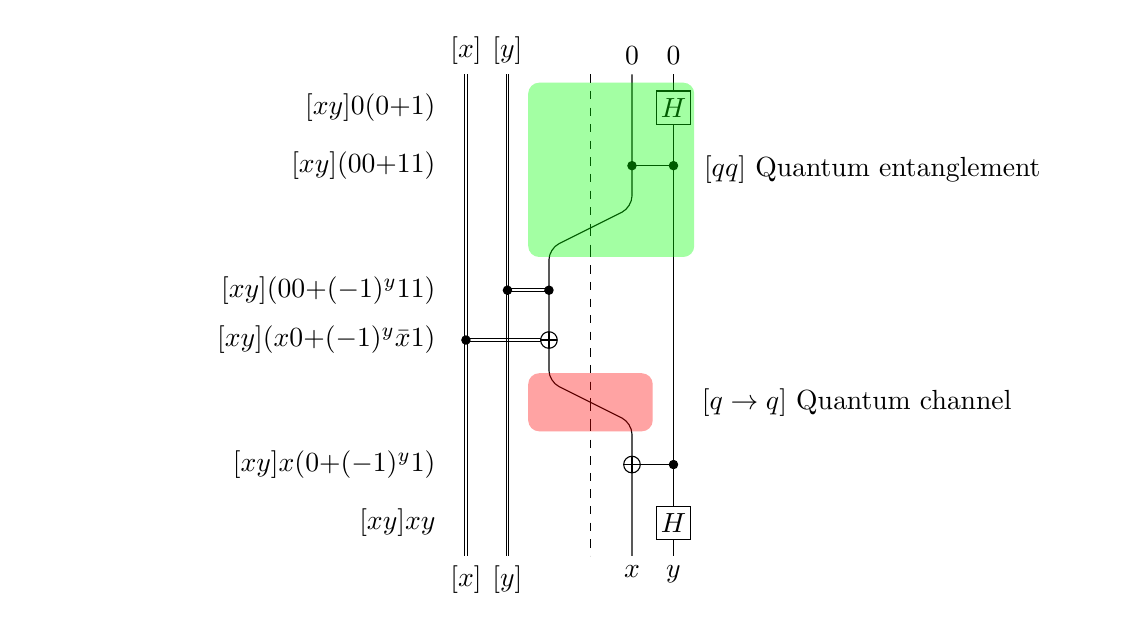
\begin{tikzpicture}[scale=1.000000,x=1pt,y=1pt]
\filldraw[color=white] (7.500000, 0.000000) rectangle (-82.500000, -174.000000);
% Drawing wires
% Line 2: a0 W [x] [x] type=c
\draw[color=black] (-74.500000,0.000000) -- (-74.500000,-174.000000);
\draw[color=black] (-75.500000,0.000000) -- (-75.500000,-174.000000);
\draw[color=black] (-75.000000,0.000000) node[above] {$[x]$};
% Line 3: a1 W [y] [y] type=c
\draw[color=black] (-59.500000,0.000000) -- (-59.500000,-174.000000);
\draw[color=black] (-60.500000,0.000000) -- (-60.500000,-174.000000);
\draw[color=black] (-60.000000,0.000000) node[above] {$[y]$};
% Line 4: x1 W type=o
% Line 5: x0 W style=dashed
\draw[color=black,dashed] (-30.000000,0.000000) -- (-30.000000,-48.000000);
\draw[color=black,dashed] (-30.000000,-48.000000) -- (-30.000000,-55.500000);
\draw[color=black,dashed] (-30.000000,-55.500000) -- (-30.000000,-63.000000);
\draw[color=black,dashed] (-30.000000,-63.000000) -- (-30.000000,-111.000000);
\draw[color=black,dashed] (-30.000000,-111.000000) -- (-30.000000,-118.500000);
\draw[color=black,dashed] (-30.000000,-118.500000) -- (-30.000000,-126.000000);
\draw[color=black,dashed] (-30.000000,-126.000000) -- (-30.000000,-174.000000);
% Line 6: b0 W \ket{0} \ket{x}
\draw[color=black,rounded corners=4.000000pt] (-15.000000,0.000000) -- (-15.000000,-48.000000) -- (-30.000000,-55.500000);
\draw[color=black,rounded corners=4.000000pt] (-30.000000,-55.500000) -- (-45.000000,-63.000000) -- (-45.000000,-111.000000) -- (-30.000000,-118.500000);
\draw[color=black,rounded corners=4.000000pt] (-30.000000,-118.500000) -- (-15.000000,-126.000000) -- (-15.000000,-174.000000);
\draw[color=black] (-15.000000,0.000000) node[above] {$\ket{0}$};
% Line 7: b1 W \ket{0} \ket{y}
\draw[color=black] (-0.000000,0.000000) -- (-0.000000,-174.000000);
\draw[color=black] (-0.000000,0.000000) node[above] {$\ket{0}$};
% Done with wires; drawing gates
% Line 10: b1 H    % $[xy]\ket{0}(\ket{0}{+}\ket{1})$
\draw (-82.500000, -12.000000) node[text width=144pt,left,text ragged left] {$[xy]\ket{0}(\ket{0}{+}\ket{1})$};
\begin{scope}
\draw[fill=white] (0.000000, -12.000000) +(-45.000000:8.485281pt and 8.485281pt) -- +(45.000000:8.485281pt and 8.485281pt) -- +(135.000000:8.485281pt and 8.485281pt) -- +(225.000000:8.485281pt and 8.485281pt) -- cycle;
\clip (0.000000, -12.000000) +(-45.000000:8.485281pt and 8.485281pt) -- +(45.000000:8.485281pt and 8.485281pt) -- +(135.000000:8.485281pt and 8.485281pt) -- +(225.000000:8.485281pt and 8.485281pt) -- cycle;
\draw (0.000000, -12.000000) node {$H$};
\end{scope}
% Line 11: b0 b1   % $[xy](\ket{00}{+}\ket{11})$
\draw (-82.500000, -33.000000) node[text width=144pt,left,text ragged left] {$[xy](\ket{00}{+}\ket{11})$};
\draw (-15.000000,-33.000000) -- (-0.000000,-33.000000);
\filldraw (-15.000000, -33.000000) circle(1.500000pt);
\filldraw (-0.000000, -33.000000) circle(1.500000pt);
% Line 12: b0 x1 PERMUTE
% Line 13: a1 b0   % $[xy](\ket{00}{+}(-1)^{y}\ket{11})$
\draw (-82.500000, -78.000000) node[text width=144pt,left,text ragged left] {$[xy](\ket{00}{+}(-1)^{y}\ket{11})$};
\draw (-60.000000,-77.500000) -- (-45.000000,-77.500000);
\draw (-60.000000,-78.500000) -- (-45.000000,-78.500000);
\filldraw (-60.000000, -78.000000) circle(1.500000pt);
\filldraw (-45.000000, -78.000000) circle(1.500000pt);
% Line 14: +b0 a0   % $[xy](\ket{x 0}{+}(-1)^{y}\ket{\bar{x} 1})$
\draw (-82.500000, -96.000000) node[text width=144pt,left,text ragged left] {$[xy](\ket{x 0}{+}(-1)^{y}\ket{\bar{x} 1})$};
\draw (-75.000000,-95.500000) -- (-45.000000,-95.500000);
\draw (-75.000000,-96.500000) -- (-45.000000,-96.500000);
\begin{scope}
\draw[fill=white] (-45.000000, -96.000000) circle(3.000000pt);
\clip (-45.000000, -96.000000) circle(3.000000pt);
\draw (-48.000000, -96.000000) -- (-42.000000, -96.000000);
\draw (-45.000000, -99.000000) -- (-45.000000, -93.000000);
\end{scope}
\filldraw (-75.000000, -96.000000) circle(1.500000pt);
% Line 15: x1 b0 PERMUTE
% Line 16: +b0 b1   % $[xy]\ket{x}(\ket{0}{+}(-1)^{y}\ket{1})$
\draw (-82.500000, -141.000000) node[text width=144pt,left,text ragged left] {$[xy]\ket{x}(\ket{0}{+}(-1)^{y}\ket{1})$};
\draw (-15.000000,-141.000000) -- (-0.000000,-141.000000);
\begin{scope}
\draw[fill=white] (-15.000000, -141.000000) circle(3.000000pt);
\clip (-15.000000, -141.000000) circle(3.000000pt);
\draw (-18.000000, -141.000000) -- (-12.000000, -141.000000);
\draw (-15.000000, -144.000000) -- (-15.000000, -138.000000);
\end{scope}
\filldraw (-0.000000, -141.000000) circle(1.500000pt);
% Line 17: b1 H    % $[xy]\ket{x y}$
\draw (-82.500000, -162.000000) node[text width=144pt,left,text ragged left] {$[xy]\ket{x y}$};
\begin{scope}
\draw[fill=white] (0.000000, -162.000000) +(-45.000000:8.485281pt and 8.485281pt) -- +(45.000000:8.485281pt and 8.485281pt) -- +(135.000000:8.485281pt and 8.485281pt) -- +(225.000000:8.485281pt and 8.485281pt) -- cycle;
\clip (0.000000, -162.000000) +(-45.000000:8.485281pt and 8.485281pt) -- +(45.000000:8.485281pt and 8.485281pt) -- +(135.000000:8.485281pt and 8.485281pt) -- +(225.000000:8.485281pt and 8.485281pt) -- cycle;
\draw (0.000000, -162.000000) node {$H$};
\end{scope}
% Done with gates; drawing ending labels
\draw[color=black] (-75.000000,-174.000000) node[below] {$[x]$};
\draw[color=black] (-60.000000,-174.000000) node[below] {$[y]$};
\draw[color=black] (-15.000000,-174.000000) node[below] {$\ket{x}$};
\draw[color=black] (-0.000000,-174.000000) node[below] {$\ket{y}$};
% Done with ending labels; drawing cut lines and comments
% Line 20: x1 b1 @ 0 2 fill=green style=rounded_corners %% $[qq]$ Quantum entanglement
\draw[draw opacity=0.000000,fill opacity=0.200000,fill=green,rounded corners] (-52.500000,-3.000000) rectangle (7.500000,-66.000000);
\draw (7.500000, -34.500000) node[text width=144pt,right] {$[qq]$ Quantum entanglement};
\draw[draw opacity=0.000000,fill opacity=0.200000,fill=green,rounded corners] (-52.500000,-3.000000) rectangle (7.500000,-66.000000);
% Line 21: b0 x1 @ 5 5 fill=red style=rounded_corners %% \hspace{.5cm}$[q\rightarrow q]$ Quantum channel
\draw[draw opacity=0.000000,fill opacity=0.200000,fill=red,rounded corners] (-52.500000,-108.000000) rectangle (-7.500000,-129.000000);
\draw (-7.500000, -118.500000) node[text width=144pt,right] {\hspace{.5cm}$[q\rightarrow q]$ Quantum channel};
\draw[draw opacity=0.000000,fill opacity=0.200000,fill=red,rounded corners] (-52.500000,-108.000000) rectangle (-7.500000,-129.000000);
% Done with comments
\end{tikzpicture}

\end{figure}
\clearpage

\SaveVerb{name}|Teleport|
\begin{figure}[ht]
\caption{\protect\UseVerb{name}}
%! \usetikzlibrary{decorations.pathreplacing,decorations.pathmorphing}
\providecommand{\ket}[1]{\left|#1\right\rangle}
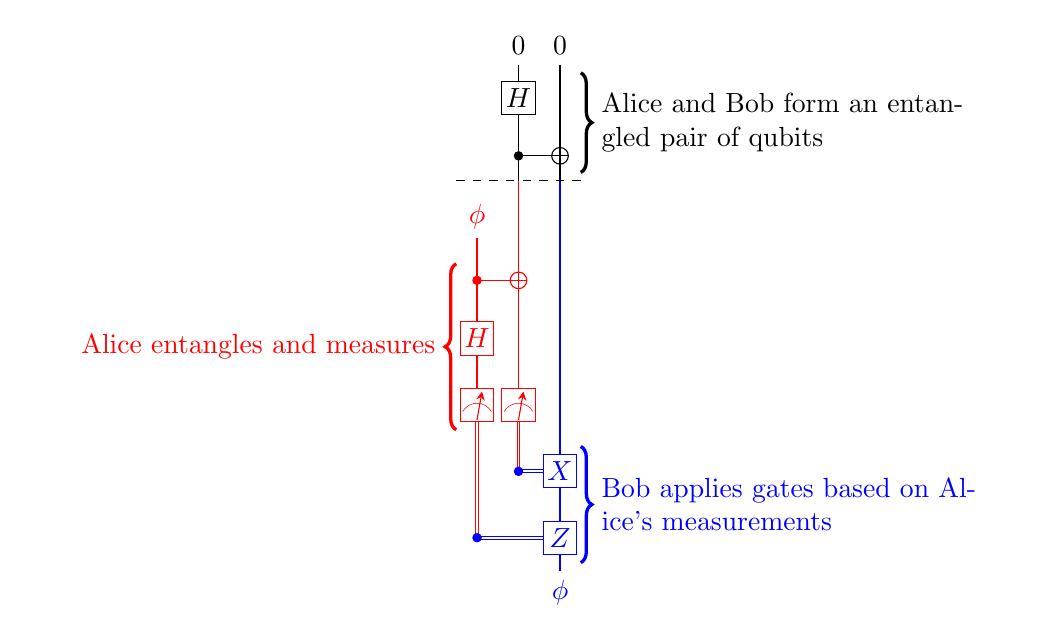
\begin{tikzpicture}[scale=1.000000,x=1pt,y=1pt]
\filldraw[color=white] (7.500000, 0.000000) rectangle (-37.500000, -183.000000);
% Drawing wires
% Line 4: 0 W \ket{\phi} color=red
\draw[color=red] (-30.000000,-55.500000) -- (-30.000000,-123.000000);
\draw[color=red] (-29.500000,-123.000000) -- (-29.500000,-171.000000);
\draw[color=red] (-30.500000,-123.000000) -- (-30.500000,-171.000000);
% Line 5: 1 W \ket{0}
\draw[color=black] (-15.000000,0.000000) -- (-15.000000,-42.000000);
\draw[color=red] (-15.000000,-42.000000) -- (-15.000000,-123.000000);
\draw[color=red] (-14.500000,-123.000000) -- (-14.500000,-147.000000);
\draw[color=red] (-15.500000,-123.000000) -- (-15.500000,-147.000000);
\draw[color=black] (-15.000000,0.000000) node[above] {$\ket{0}$};
% Line 6: 2 W \ket{0} \ket{\phi}
\draw[color=black] (-0.000000,0.000000) -- (-0.000000,-42.000000);
\draw[color=blue] (-0.000000,-42.000000) -- (-0.000000,-183.000000);
\draw[color=black] (-0.000000,0.000000) node[above] {$\ket{0}$};
% Done with wires; drawing gates
% Line 8: 1 H
\begin{scope}
\draw[fill=white] (-15.000000, -12.000000) +(-45.000000:8.485281pt and 8.485281pt) -- +(45.000000:8.485281pt and 8.485281pt) -- +(135.000000:8.485281pt and 8.485281pt) -- +(225.000000:8.485281pt and 8.485281pt) -- cycle;
\clip (-15.000000, -12.000000) +(-45.000000:8.485281pt and 8.485281pt) -- +(45.000000:8.485281pt and 8.485281pt) -- +(135.000000:8.485281pt and 8.485281pt) -- +(225.000000:8.485281pt and 8.485281pt) -- cycle;
\draw (-15.000000, -12.000000) node {$H$};
\end{scope}
% Line 9: +2 1
\draw (-15.000000,-33.000000) -- (-0.000000,-33.000000);
\begin{scope}
\draw[fill=white] (-0.000000, -33.000000) circle(3.000000pt);
\clip (-0.000000, -33.000000) circle(3.000000pt);
\draw (-3.000000, -33.000000) -- (3.000000, -33.000000);
\draw (-0.000000, -36.000000) -- (-0.000000, -30.000000);
\end{scope}
\filldraw (-15.000000, -33.000000) circle(1.500000pt);
% Line 12: TOUCH
% Line 13: 1:color=red 2:color=blue TOUCH
% Line 14: 0 START
\draw[color=red] (-30.000000,-63.000000) node[fill=white,above,minimum width=15.000000pt,minimum height=15.000000pt,inner sep=0pt] {\phantom{$\ket{\phi}$}};
\draw[color=red] (-30.000000,-63.000000) node[above] {$\ket{\phi}$};
% Line 18: +1 0 color=red
\begin{scope}[color=red]
\draw (-30.000000,-78.000000) -- (-15.000000,-78.000000);
\begin{scope}
\draw[fill=white] (-15.000000, -78.000000) circle(3.000000pt);
\clip (-15.000000, -78.000000) circle(3.000000pt);
\draw (-18.000000, -78.000000) -- (-12.000000, -78.000000);
\draw (-15.000000, -81.000000) -- (-15.000000, -75.000000);
\end{scope}
\filldraw (-30.000000, -78.000000) circle(1.500000pt);
\end{scope}
% Line 19: 0 H color=red
\begin{scope}[color=red]
\begin{scope}[color=red]
\begin{scope}
\draw[fill=white] (-30.000000, -99.000000) +(-45.000000:8.485281pt and 8.485281pt) -- +(45.000000:8.485281pt and 8.485281pt) -- +(135.000000:8.485281pt and 8.485281pt) -- +(225.000000:8.485281pt and 8.485281pt) -- cycle;
\clip (-30.000000, -99.000000) +(-45.000000:8.485281pt and 8.485281pt) -- +(45.000000:8.485281pt and 8.485281pt) -- +(135.000000:8.485281pt and 8.485281pt) -- +(225.000000:8.485281pt and 8.485281pt) -- cycle;
\draw (-30.000000, -99.000000) node {$H$};
\end{scope}
\end{scope}
\end{scope}
% Line 20: 1 TOUCH
% Line 21: 0 M color=red
\begin{scope}[color=red]
\draw[fill=white] (-36.000000, -129.000000) rectangle (-24.000000, -117.000000);
\draw[very thin] (-30.000000, -122.400000) arc (90:150:6.000000pt);
\draw[very thin] (-30.000000, -122.400000) arc (90:30:6.000000pt);
\draw[->,>=stealth] (-30.000000, -128.400000) -- +(80:10.392305pt);
\end{scope}
% Line 22: 1 M color=red
\begin{scope}[color=red]
\draw[fill=white] (-21.000000, -129.000000) rectangle (-9.000000, -117.000000);
\draw[very thin] (-15.000000, -122.400000) arc (90:150:6.000000pt);
\draw[very thin] (-15.000000, -122.400000) arc (90:30:6.000000pt);
\draw[->,>=stealth] (-15.000000, -128.400000) -- +(80:10.392305pt);
\end{scope}
% Line 26: 2 X 1:type=o co=blue
\begin{scope}[color=blue]
\draw (-15.000000,-146.500000) -- (-0.000000,-146.500000);
\draw (-15.000000,-147.500000) -- (-0.000000,-147.500000);
\begin{scope}[color=blue]
\begin{scope}
\draw[fill=white] (0.000000, -147.000000) +(-45.000000:8.485281pt and 8.485281pt) -- +(45.000000:8.485281pt and 8.485281pt) -- +(135.000000:8.485281pt and 8.485281pt) -- +(225.000000:8.485281pt and 8.485281pt) -- cycle;
\clip (0.000000, -147.000000) +(-45.000000:8.485281pt and 8.485281pt) -- +(45.000000:8.485281pt and 8.485281pt) -- +(135.000000:8.485281pt and 8.485281pt) -- +(225.000000:8.485281pt and 8.485281pt) -- cycle;
\draw (0.000000, -147.000000) node {$X$};
\end{scope}
\end{scope}
\filldraw (-15.000000, -147.000000) circle(1.500000pt);
\end{scope}
% Line 27: 2 Z 0:type=o co=blue
\begin{scope}[color=blue]
\draw (-30.000000,-170.500000) -- (-0.000000,-170.500000);
\draw (-30.000000,-171.500000) -- (-0.000000,-171.500000);
\begin{scope}[color=blue]
\begin{scope}
\draw[fill=white] (0.000000, -171.000000) +(-45.000000:8.485281pt and 8.485281pt) -- +(45.000000:8.485281pt and 8.485281pt) -- +(135.000000:8.485281pt and 8.485281pt) -- +(225.000000:8.485281pt and 8.485281pt) -- cycle;
\clip (0.000000, -171.000000) +(-45.000000:8.485281pt and 8.485281pt) -- +(45.000000:8.485281pt and 8.485281pt) -- +(135.000000:8.485281pt and 8.485281pt) -- +(225.000000:8.485281pt and 8.485281pt) -- cycle;
\draw (0.000000, -171.000000) node {$Z$};
\end{scope}
\end{scope}
\filldraw (-30.000000, -171.000000) circle(1.500000pt);
\end{scope}
% Done with gates; drawing ending labels
\draw[color=blue] (-0.000000,-183.000000) node[below] {$\ket{\phi}$};
% Done with ending labels; drawing cut lines and comments
\draw[dashed] (7.500000, -42.000000) -- (-37.500000, -42.000000);
% Line 10: @ 2 %% Alice and Bob form an entangled pair of qubits
\draw[decorate,decoration={brace,amplitude = 4.000000pt},very thick] (7.500000,-3.000000) -- (7.500000,-39.000000);
\draw (11.500000, -21.000000) node[text width=144pt,right] {Alice and Bob form an entangled pair of qubits};
% Line 23: @ Astart color=red % Alice entangles and measures
\draw[decorate,decoration={brace,mirror,amplitude = 4.000000pt},very thick,color=red] (-37.500000,-72.000000) -- (-37.500000,-132.000000);
\draw (-41.500000, -102.000000) node[text width=144pt,left,text ragged left,color=red] {Alice entangles and measures};
% Line 28: @ Bstart color=blue %% Bob applies gates based on Alice's measurements
\draw[decorate,decoration={brace,amplitude = 4.000000pt},very thick,color=blue] (7.500000,-138.000000) -- (7.500000,-180.000000);
\draw (11.500000, -159.000000) node[text width=144pt,right,color=blue] {Bob applies gates based on Alice's measurements};
% Done with comments
\end{tikzpicture}

\end{figure}

\SaveVerb{name}|boxtest|
\begin{figure}[ht]
\caption{\protect\UseVerb{name}}
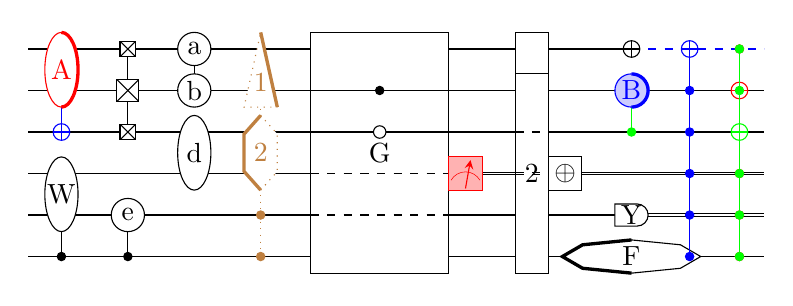
\begin{tikzpicture}[scale=1.000000,x=1pt,y=1pt]
\filldraw[color=white] (0.000000, -7.500000) rectangle (266.000000, 82.500000);
% Drawing wires
% Line 4: a W
\draw[color=black] (0.000000,75.000000) -- (218.000000,75.000000);
\draw[color=blue,dashed] (218.000000,75.000000) -- (266.000000,75.000000);
% Line 5: b W
\draw[color=black] (0.000000,60.000000) -- (266.000000,60.000000);
% Line 6: c W
\draw[color=black] (0.000000,45.000000) -- (266.000000,45.000000);
% Line 7: d W
\draw[color=black] (0.000000,30.000000) -- (158.000000,30.000000);
\draw[color=black] (158.000000,29.500000) -- (266.000000,29.500000);
\draw[color=black] (158.000000,30.500000) -- (266.000000,30.500000);
% Line 8: e W
\draw[color=black] (0.000000,15.000000) -- (218.000000,15.000000);
\draw[color=black] (218.000000,14.500000) -- (266.000000,14.500000);
\draw[color=black] (218.000000,15.500000) -- (266.000000,15.500000);
% Line 9: f W
\draw[color=black] (0.000000,0.000000) -- (266.000000,0.000000);
% Done with wires; drawing gates
% Line 13: a b G|:color=red A +c color=blue shape=circle
\begin{scope}[color=blue]
\draw (12.000000,75.000000) -- (12.000000,45.000000);
\begin{scope}[color=red]
\begin{scope}
\draw[fill=white] (12.000000, 67.500000) ellipse(6.000000pt and 13.500000pt);
\draw[very thick,solid] (12.000000, 67.500000) +(-90.000000:6.000000pt and 13.500000pt) arc (-90.000000:90.000000:6.000000pt and 13.500000pt);
\clip (12.000000, 67.500000) ellipse(6.000000pt and 13.500000pt);
\draw (12.000000, 67.500000) node {A};
\end{scope}
\end{scope}
\begin{scope}
\draw[fill=white] (12.000000, 45.000000) circle(3.000000pt);
\clip (12.000000, 45.000000) circle(3.000000pt);
\draw (9.000000, 45.000000) -- (15.000000, 45.000000);
\draw (12.000000, 42.000000) -- (12.000000, 48.000000);
\end{scope}
\end{scope}
% Line 14: +d e P W f
\draw (12.000000,30.000000) -- (12.000000,0.000000);
\begin{scope}
\draw[fill=white] (12.000000, 22.500000) ellipse(6.000000pt and 13.500000pt);
\clip (12.000000, 22.500000) ellipse(6.000000pt and 13.500000pt);
\draw (12.000000, 22.500000) node {W};
\end{scope}
\filldraw (12.000000, 0.000000) circle(1.500000pt);
% Line 15: a P:shape=4:size=8 x b G:shape=4:size=8 x +c:shape=4:size=8:op=x
\draw (36.000000,75.000000) -- (36.000000,45.000000);
\begin{scope}
\draw[fill=white] (36.000000, 75.000000) +(-45.000000:4.000000pt) -- +(45.000000:4.000000pt) -- +(135.000000:4.000000pt) -- +(225.000000:4.000000pt) -- cycle;
\clip (36.000000, 75.000000) +(-45.000000:4.000000pt) -- +(45.000000:4.000000pt) -- +(135.000000:4.000000pt) -- +(225.000000:4.000000pt) -- cycle;
\draw (33.171573, 72.171573) -- (38.828427, 77.828427);
\draw (33.171573, 77.828427) -- (38.828427, 72.171573);
\end{scope}
\begin{scope}
\draw[fill=white] (36.000000, 60.000000) +(-45.000000:5.656854pt and 5.656854pt) -- +(45.000000:5.656854pt and 5.656854pt) -- +(135.000000:5.656854pt and 5.656854pt) -- +(225.000000:5.656854pt and 5.656854pt) -- cycle;
\clip (36.000000, 60.000000) +(-45.000000:5.656854pt and 5.656854pt) -- +(45.000000:5.656854pt and 5.656854pt) -- +(135.000000:5.656854pt and 5.656854pt) -- +(225.000000:5.656854pt and 5.656854pt) -- cycle;
\draw (32.000000, 56.000000) -- (40.000000, 64.000000);
\draw (32.000000, 64.000000) -- (40.000000, 56.000000);
\end{scope}
\begin{scope}
\draw[fill=white] (36.000000, 45.000000) +(-45.000000:4.000000pt) -- +(45.000000:4.000000pt) -- +(135.000000:4.000000pt) -- +(225.000000:4.000000pt) -- cycle;
\clip (36.000000, 45.000000) +(-45.000000:4.000000pt) -- +(45.000000:4.000000pt) -- +(135.000000:4.000000pt) -- +(225.000000:4.000000pt) -- cycle;
\draw (33.171573, 42.171573) -- (38.828427, 47.828427);
\draw (33.171573, 47.828427) -- (38.828427, 42.171573);
\end{scope}
% Line 16: e P e f
\draw (36.000000,15.000000) -- (36.000000,0.000000);
\begin{scope}
\draw[fill=white] (36.000000, 15.000000) circle(6.000000pt);
\clip (36.000000, 15.000000) circle(6.000000pt);
\draw (36.000000, 15.000000) node {e};
\end{scope}
\filldraw (36.000000, 0.000000) circle(1.500000pt);
% Line 17: a P a b P b
\draw (60.000000,75.000000) -- (60.000000,60.000000);
\begin{scope}
\draw[fill=white] (60.000000, 75.000000) circle(6.000000pt);
\clip (60.000000, 75.000000) circle(6.000000pt);
\draw (60.000000, 75.000000) node {a};
\end{scope}
\begin{scope}
\draw[fill=white] (60.000000, 60.000000) circle(6.000000pt);
\clip (60.000000, 60.000000) circle(6.000000pt);
\draw (60.000000, 60.000000) node {b};
\end{scope}
% Line 19: c d P d
\draw (60.000000,45.000000) -- (60.000000,30.000000);
\begin{scope}
\draw[fill=white] (60.000000, 37.500000) ellipse(6.000000pt and 13.500000pt);
\clip (60.000000, 37.500000) ellipse(6.000000pt and 13.500000pt);
\draw (60.000000, 37.500000) node {d};
\end{scope}
% Line 21: a b G|:shape=3 1 c d |G:shape=-6 2 e f style=dotted color=brown
\begin{scope}[color=brown]
\draw[dotted] (84.000000,75.000000) -- (84.000000,0.000000);
\begin{scope}[color=brown,dotted]
\begin{scope}
\draw[fill=white] (84.000000, 63.000000) +(-30.000000:6.928203pt and 18.000000pt) -- +(90.000000:6.928203pt and 18.000000pt) -- +(210.000000:6.928203pt and 18.000000pt) -- cycle;
\draw[very thick,solid] (84.000000, 63.000000) +(-30.000000:6.928203pt and 18.000000pt) -- +(90.000000:6.928203pt and 18.000000pt);
\clip (84.000000, 63.000000) +(-30.000000:6.928203pt and 18.000000pt) -- +(90.000000:6.928203pt and 18.000000pt) -- +(210.000000:6.928203pt and 18.000000pt) -- cycle;
\draw (84.000000, 63.000000) node {1};
\end{scope}
\end{scope}
\begin{scope}[color=brown,dotted]
\begin{scope}
\draw[fill=white] (84.000000, 37.500000) +(-90.000000:6.928203pt and 13.500000pt) -- +(-30.000000:6.928203pt and 13.500000pt) -- +(30.000000:6.928203pt and 13.500000pt) -- +(90.000000:6.928203pt and 13.500000pt) -- +(150.000000:6.928203pt and 13.500000pt) -- +(210.000000:6.928203pt and 13.500000pt) -- cycle;
\draw[very thick,solid] (84.000000, 37.500000) +(90.000000:6.928203pt and 13.500000pt) -- +(150.000000:6.928203pt and 13.500000pt) -- +(210.000000:6.928203pt and 13.500000pt) -- +(-90.000000:6.928203pt and 13.500000pt);
\clip (84.000000, 37.500000) +(-90.000000:6.928203pt and 13.500000pt) -- +(-30.000000:6.928203pt and 13.500000pt) -- +(30.000000:6.928203pt and 13.500000pt) -- +(90.000000:6.928203pt and 13.500000pt) -- +(150.000000:6.928203pt and 13.500000pt) -- +(210.000000:6.928203pt and 13.500000pt) -- cycle;
\draw (84.000000, 37.500000) node {2};
\end{scope}
\end{scope}
\filldraw (84.000000, 15.000000) circle(1.500000pt);
\filldraw (84.000000, 0.000000) circle(1.500000pt);
\end{scope}
% Line 23: a f G G b -c width=50
\draw (127.000000,75.000000) -- (127.000000,0.000000);
\begin{scope}
\draw[fill=white] (127.000000, 37.500000) +(-45.000000:35.355339pt and 61.518290pt) -- +(45.000000:35.355339pt and 61.518290pt) -- +(135.000000:35.355339pt and 61.518290pt) -- +(225.000000:35.355339pt and 61.518290pt) -- cycle;
\clip (127.000000, 37.500000) +(-45.000000:35.355339pt and 61.518290pt) -- +(45.000000:35.355339pt and 61.518290pt) -- +(135.000000:35.355339pt and 61.518290pt) -- +(225.000000:35.355339pt and 61.518290pt) -- cycle;
\draw (127.000000, 37.500000) node {G};
\end{scope}
\draw[color=black] (102.000000, 60.000000) -- (152.000000, 60.000000);
\draw[color=black] (102.000000, 45.000000) -- (152.000000, 45.000000);
\draw[color=black,dashed] (102.000000, 30.000000) -- (152.000000, 30.000000);
\draw[color=black,dashed] (102.000000, 15.000000) -- (152.000000, 15.000000);
\filldraw (127.000000, 60.000000) circle(1.500000pt);
\draw[fill=white] (127.000000, 45.000000) circle(2.250000pt);
% Line 31: d M:fill=red!30!white color=red
\begin{scope}[color=red]
\draw[fill=red!30!white] (152.000000, 24.000000) rectangle (164.000000, 36.000000);
\draw[very thin] (158.000000, 30.600000) arc (90:150:6.000000pt);
\draw[very thin] (158.000000, 30.600000) arc (90:30:6.000000pt);
\draw[->,>=stealth] (158.000000, 24.600000) -- +(80:10.392305pt);
\end{scope}
% Line 25: a e G 1 b f G 2
\draw (182.000000,75.000000) -- (182.000000,0.000000);
\begin{scope}
\draw[fill=white] (182.000000, 45.000000) +(-45.000000:8.485281pt and 50.911688pt) -- +(45.000000:8.485281pt and 50.911688pt) -- +(135.000000:8.485281pt and 50.911688pt) -- +(225.000000:8.485281pt and 50.911688pt) -- cycle;
\clip (182.000000, 45.000000) +(-45.000000:8.485281pt and 50.911688pt) -- +(45.000000:8.485281pt and 50.911688pt) -- +(135.000000:8.485281pt and 50.911688pt) -- +(225.000000:8.485281pt and 50.911688pt) -- cycle;
\draw (182.000000, 45.000000) node {1};
\end{scope}
\begin{scope}
\draw[fill=white] (182.000000, 30.000000) +(-45.000000:8.485281pt and 50.911688pt) -- +(45.000000:8.485281pt and 50.911688pt) -- +(135.000000:8.485281pt and 50.911688pt) -- +(225.000000:8.485281pt and 50.911688pt) -- cycle;
\clip (182.000000, 30.000000) +(-45.000000:8.485281pt and 50.911688pt) -- +(45.000000:8.485281pt and 50.911688pt) -- +(135.000000:8.485281pt and 50.911688pt) -- +(225.000000:8.485281pt and 50.911688pt) -- cycle;
\draw (182.000000, 30.000000) node {2};
\end{scope}
\draw[color=black,dashed] (176.000000, 45.000000) -- (188.000000, 45.000000);
\draw[color=black,dashed] (176.000000, 29.500000) -- (188.000000, 29.500000);
\draw[color=black,dashed] (176.000000, 30.500000) -- (188.000000, 30.500000);
% Line 33: d G $\oplus$
\begin{scope}
\draw[fill=white] (194.000000, 30.000000) +(-45.000000:8.485281pt and 8.485281pt) -- +(45.000000:8.485281pt and 8.485281pt) -- +(135.000000:8.485281pt and 8.485281pt) -- +(225.000000:8.485281pt and 8.485281pt) -- cycle;
\clip (194.000000, 30.000000) +(-45.000000:8.485281pt and 8.485281pt) -- +(45.000000:8.485281pt and 8.485281pt) -- +(135.000000:8.485281pt and 8.485281pt) -- +(225.000000:8.485281pt and 8.485281pt) -- cycle;
\draw (194.000000, 30.000000) node {$\oplus$};
\end{scope}
% Line 27: +a1:style=dashed
\begin{scope}
\draw[fill=white] (218.000000, 75.000000) circle(3.000000pt);
\clip (218.000000, 75.000000) circle(3.000000pt);
\draw (215.000000, 75.000000) -- (221.000000, 75.000000);
\draw (218.000000, 72.000000) -- (218.000000, 78.000000);
\end{scope}
% Line 29: b G1:fill=blue!20!white:shape=circle color=green B c
\begin{scope}[color=green]
\draw (218.000000,60.000000) -- (218.000000,45.000000);
\begin{scope}[color=blue]
\begin{scope}
\draw[fill=blue!20!white] (218.000000, 60.000000) circle(6.000000pt);
\draw[very thick,solid] (218.000000, 60.000000) +(-90.000000:6.000000pt) arc (-90.000000:90.000000:6.000000pt);
\clip (218.000000, 60.000000) circle(6.000000pt);
\draw (218.000000, 60.000000) node {B};
\end{scope}
\end{scope}
\filldraw (218.000000, 45.000000) circle(1.500000pt);
\end{scope}
% Line 34: e M:op=Y A B
\draw[fill=white] (212.000000, 11.000000) -- (220.000000,11.000000) arc (-90:90:4.000000pt) -- (212.000000,19.000000) -- cycle;
\draw (218.000000, 15.000000) node {Y};
% Line 36: f |G:width=50:op=F:shape=-8 width=5
\begin{scope}
\draw[fill=white] (218.000000, 0.000000) +(-90.000000:25.000000pt and 6.000000pt) -- +(-45.000000:25.000000pt and 6.000000pt) -- +(0.000000:25.000000pt and 6.000000pt) -- +(45.000000:25.000000pt and 6.000000pt) -- +(90.000000:25.000000pt and 6.000000pt) -- +(135.000000:25.000000pt and 6.000000pt) -- +(180.000000:25.000000pt and 6.000000pt) -- +(225.000000:25.000000pt and 6.000000pt) -- cycle;
\draw[very thick,solid] (218.000000, 0.000000) +(90.000000:25.000000pt and 6.000000pt) -- +(135.000000:25.000000pt and 6.000000pt) -- +(180.000000:25.000000pt and 6.000000pt) -- +(180.000000:25.000000pt and 6.000000pt) -- +(225.000000:25.000000pt and 6.000000pt) -- +(-90.000000:25.000000pt and 6.000000pt);
\clip (218.000000, 0.000000) +(-90.000000:25.000000pt and 6.000000pt) -- +(-45.000000:25.000000pt and 6.000000pt) -- +(0.000000:25.000000pt and 6.000000pt) -- +(45.000000:25.000000pt and 6.000000pt) -- +(90.000000:25.000000pt and 6.000000pt) -- +(135.000000:25.000000pt and 6.000000pt) -- +(180.000000:25.000000pt and 6.000000pt) -- +(225.000000:25.000000pt and 6.000000pt) -- cycle;
\draw (218.000000, 0.000000) node {F};
\end{scope}
% Line 38: +a b c d e f color=blue
\begin{scope}[color=blue]
\draw (239.000000,75.000000) -- (239.000000,0.000000);
\begin{scope}
\draw[fill=white] (239.000000, 75.000000) circle(3.000000pt);
\clip (239.000000, 75.000000) circle(3.000000pt);
\draw (236.000000, 75.000000) -- (242.000000, 75.000000);
\draw (239.000000, 72.000000) -- (239.000000, 78.000000);
\end{scope}
\filldraw (239.000000, 60.000000) circle(1.500000pt);
\filldraw (239.000000, 45.000000) circle(1.500000pt);
\filldraw (239.000000, 30.000000) circle(1.500000pt);
\filldraw (239.000000, 15.000000) circle(1.500000pt);
\filldraw (239.000000, 0.000000) circle(1.500000pt);
\end{scope}
% Line 39: +b a c d e f color=red
\begin{scope}[color=red]
\draw (257.000000,75.000000) -- (257.000000,0.000000);
\begin{scope}
\draw[fill=white] (257.000000, 60.000000) circle(3.000000pt);
\clip (257.000000, 60.000000) circle(3.000000pt);
\draw (254.000000, 60.000000) -- (260.000000, 60.000000);
\draw (257.000000, 57.000000) -- (257.000000, 63.000000);
\end{scope}
\filldraw (257.000000, 75.000000) circle(1.500000pt);
\filldraw (257.000000, 45.000000) circle(1.500000pt);
\filldraw (257.000000, 30.000000) circle(1.500000pt);
\filldraw (257.000000, 15.000000) circle(1.500000pt);
\filldraw (257.000000, 0.000000) circle(1.500000pt);
\end{scope}
% Line 40: LABEL length=-30
% Line 41: +c a b d e f color=green
\begin{scope}[color=green]
\draw (257.000000,75.000000) -- (257.000000,0.000000);
\begin{scope}
\draw[fill=white] (257.000000, 45.000000) circle(3.000000pt);
\clip (257.000000, 45.000000) circle(3.000000pt);
\draw (254.000000, 45.000000) -- (260.000000, 45.000000);
\draw (257.000000, 42.000000) -- (257.000000, 48.000000);
\end{scope}
\filldraw (257.000000, 75.000000) circle(1.500000pt);
\filldraw (257.000000, 60.000000) circle(1.500000pt);
\filldraw (257.000000, 30.000000) circle(1.500000pt);
\filldraw (257.000000, 15.000000) circle(1.500000pt);
\filldraw (257.000000, 0.000000) circle(1.500000pt);
\end{scope}
% Done with gates; drawing ending labels
% Done with ending labels; drawing cut lines and comments
% Done with comments
\end{tikzpicture}

\end{figure}

\SaveVerb{name}|cswap|
\begin{figure}[ht]
\caption{\protect\UseVerb{name}}
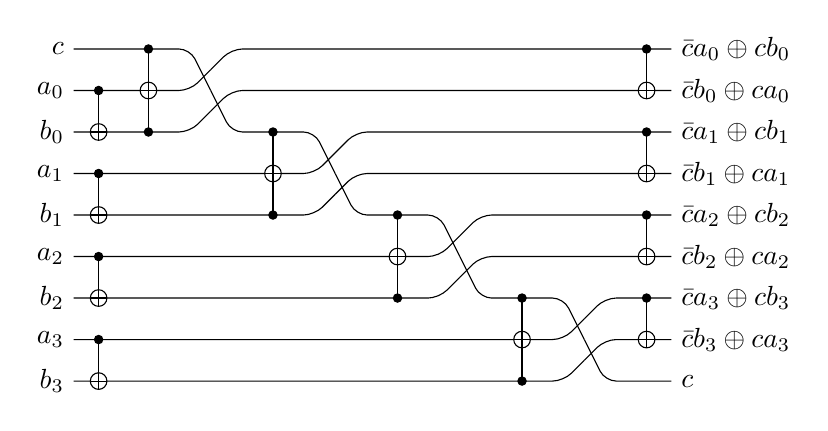
\begin{tikzpicture}[scale=1.000000,x=1pt,y=1pt]
\filldraw[color=white] (0.000000, -7.500000) rectangle (216.000000, 127.500000);
% Drawing wires
% Line 1: c W c c
\draw[color=black,rounded corners=4.000000pt] (0.000000,120.000000) -- (42.000000,120.000000) -- (49.500000,105.000000);
\draw[color=black,rounded corners=4.000000pt] (49.500000,105.000000) -- (57.000000,90.000000) -- (87.000000,90.000000) -- (94.500000,75.000000);
\draw[color=black,rounded corners=4.000000pt] (94.500000,75.000000) -- (102.000000,60.000000) -- (132.000000,60.000000) -- (139.500000,45.000000);
\draw[color=black,rounded corners=4.000000pt] (139.500000,45.000000) -- (147.000000,30.000000) -- (177.000000,30.000000) -- (184.500000,15.000000);
\draw[color=black,rounded corners=4.000000pt] (184.500000,15.000000) -- (192.000000,0.000000) -- (216.000000,0.000000);
\draw[color=black] (0.000000,120.000000) node[left] {$c$};
% Line 2: a0 W a_0 {\bar c a_0 \oplus c b_0}
\draw[color=black,rounded corners=4.000000pt] (0.000000,105.000000) -- (42.000000,105.000000) -- (49.500000,112.500000);
\draw[color=black,rounded corners=4.000000pt] (49.500000,112.500000) -- (57.000000,120.000000) -- (216.000000,120.000000);
\draw[color=black] (0.000000,105.000000) node[left] {$a_0$};
% Line 3: b0 W b_0 {\bar c b_0 \oplus c a_0}
\draw[color=black,rounded corners=4.000000pt] (0.000000,90.000000) -- (42.000000,90.000000) -- (49.500000,97.500000);
\draw[color=black,rounded corners=4.000000pt] (49.500000,97.500000) -- (57.000000,105.000000) -- (216.000000,105.000000);
\draw[color=black] (0.000000,90.000000) node[left] {$b_0$};
% Line 4: a1 W a_1 {\bar c a_1 \oplus c b_1}
\draw[color=black,rounded corners=4.000000pt] (0.000000,75.000000) -- (87.000000,75.000000) -- (94.500000,82.500000);
\draw[color=black,rounded corners=4.000000pt] (94.500000,82.500000) -- (102.000000,90.000000) -- (216.000000,90.000000);
\draw[color=black] (0.000000,75.000000) node[left] {$a_1$};
% Line 5: b1 W b_1 {\bar c b_1 \oplus c a_1}
\draw[color=black,rounded corners=4.000000pt] (0.000000,60.000000) -- (87.000000,60.000000) -- (94.500000,67.500000);
\draw[color=black,rounded corners=4.000000pt] (94.500000,67.500000) -- (102.000000,75.000000) -- (216.000000,75.000000);
\draw[color=black] (0.000000,60.000000) node[left] {$b_1$};
% Line 6: a2 W a_2 {\bar c a_2 \oplus c b_2}
\draw[color=black,rounded corners=4.000000pt] (0.000000,45.000000) -- (132.000000,45.000000) -- (139.500000,52.500000);
\draw[color=black,rounded corners=4.000000pt] (139.500000,52.500000) -- (147.000000,60.000000) -- (216.000000,60.000000);
\draw[color=black] (0.000000,45.000000) node[left] {$a_2$};
% Line 7: b2 W b_2 {\bar c b_2 \oplus c a_2}
\draw[color=black,rounded corners=4.000000pt] (0.000000,30.000000) -- (132.000000,30.000000) -- (139.500000,37.500000);
\draw[color=black,rounded corners=4.000000pt] (139.500000,37.500000) -- (147.000000,45.000000) -- (216.000000,45.000000);
\draw[color=black] (0.000000,30.000000) node[left] {$b_2$};
% Line 8: a3 W a_3 {\bar c a_3 \oplus c b_3}
\draw[color=black,rounded corners=4.000000pt] (0.000000,15.000000) -- (177.000000,15.000000) -- (184.500000,22.500000);
\draw[color=black,rounded corners=4.000000pt] (184.500000,22.500000) -- (192.000000,30.000000) -- (216.000000,30.000000);
\draw[color=black] (0.000000,15.000000) node[left] {$a_3$};
% Line 9: b3 W b_3 {\bar c b_3 \oplus c a_3}
\draw[color=black,rounded corners=4.000000pt] (0.000000,0.000000) -- (177.000000,0.000000) -- (184.500000,7.500000);
\draw[color=black,rounded corners=4.000000pt] (184.500000,7.500000) -- (192.000000,15.000000) -- (216.000000,15.000000);
\draw[color=black] (0.000000,0.000000) node[left] {$b_3$};
% Done with wires; drawing gates
% Line 11: +b0 a0
\draw (9.000000,105.000000) -- (9.000000,90.000000);
\begin{scope}
\draw[fill=white] (9.000000, 90.000000) circle(3.000000pt);
\clip (9.000000, 90.000000) circle(3.000000pt);
\draw (6.000000, 90.000000) -- (12.000000, 90.000000);
\draw (9.000000, 87.000000) -- (9.000000, 93.000000);
\end{scope}
\filldraw (9.000000, 105.000000) circle(1.500000pt);
\draw (207.000000,120.000000) -- (207.000000,105.000000);
\begin{scope}
\draw[fill=white] (207.000000, 105.000000) circle(3.000000pt);
\clip (207.000000, 105.000000) circle(3.000000pt);
\draw (204.000000, 105.000000) -- (210.000000, 105.000000);
\draw (207.000000, 102.000000) -- (207.000000, 108.000000);
\end{scope}
\filldraw (207.000000, 120.000000) circle(1.500000pt);
% Line 12: +b1 a1
\draw (9.000000,75.000000) -- (9.000000,60.000000);
\begin{scope}
\draw[fill=white] (9.000000, 60.000000) circle(3.000000pt);
\clip (9.000000, 60.000000) circle(3.000000pt);
\draw (6.000000, 60.000000) -- (12.000000, 60.000000);
\draw (9.000000, 57.000000) -- (9.000000, 63.000000);
\end{scope}
\filldraw (9.000000, 75.000000) circle(1.500000pt);
\draw (207.000000,90.000000) -- (207.000000,75.000000);
\begin{scope}
\draw[fill=white] (207.000000, 75.000000) circle(3.000000pt);
\clip (207.000000, 75.000000) circle(3.000000pt);
\draw (204.000000, 75.000000) -- (210.000000, 75.000000);
\draw (207.000000, 72.000000) -- (207.000000, 78.000000);
\end{scope}
\filldraw (207.000000, 90.000000) circle(1.500000pt);
% Line 13: +b2 a2
\draw (9.000000,45.000000) -- (9.000000,30.000000);
\begin{scope}
\draw[fill=white] (9.000000, 30.000000) circle(3.000000pt);
\clip (9.000000, 30.000000) circle(3.000000pt);
\draw (6.000000, 30.000000) -- (12.000000, 30.000000);
\draw (9.000000, 27.000000) -- (9.000000, 33.000000);
\end{scope}
\filldraw (9.000000, 45.000000) circle(1.500000pt);
\draw (207.000000,60.000000) -- (207.000000,45.000000);
\begin{scope}
\draw[fill=white] (207.000000, 45.000000) circle(3.000000pt);
\clip (207.000000, 45.000000) circle(3.000000pt);
\draw (204.000000, 45.000000) -- (210.000000, 45.000000);
\draw (207.000000, 42.000000) -- (207.000000, 48.000000);
\end{scope}
\filldraw (207.000000, 60.000000) circle(1.500000pt);
% Line 14: +b3 a3
\draw (9.000000,15.000000) -- (9.000000,0.000000);
\begin{scope}
\draw[fill=white] (9.000000, 0.000000) circle(3.000000pt);
\clip (9.000000, 0.000000) circle(3.000000pt);
\draw (6.000000, 0.000000) -- (12.000000, 0.000000);
\draw (9.000000, -3.000000) -- (9.000000, 3.000000);
\end{scope}
\filldraw (9.000000, 15.000000) circle(1.500000pt);
\draw (207.000000,30.000000) -- (207.000000,15.000000);
\begin{scope}
\draw[fill=white] (207.000000, 15.000000) circle(3.000000pt);
\clip (207.000000, 15.000000) circle(3.000000pt);
\draw (204.000000, 15.000000) -- (210.000000, 15.000000);
\draw (207.000000, 12.000000) -- (207.000000, 18.000000);
\end{scope}
\filldraw (207.000000, 30.000000) circle(1.500000pt);
% Line 16: +a0 b0 c
\draw (27.000000,120.000000) -- (27.000000,90.000000);
\begin{scope}
\draw[fill=white] (27.000000, 105.000000) circle(3.000000pt);
\clip (27.000000, 105.000000) circle(3.000000pt);
\draw (24.000000, 105.000000) -- (30.000000, 105.000000);
\draw (27.000000, 102.000000) -- (27.000000, 108.000000);
\end{scope}
\filldraw (27.000000, 90.000000) circle(1.500000pt);
\filldraw (27.000000, 120.000000) circle(1.500000pt);
% Line 17: a0 b0 c PERMUTE
% Line 18: +a1 b1 c
\draw (72.000000,90.000000) -- (72.000000,60.000000);
\begin{scope}
\draw[fill=white] (72.000000, 75.000000) circle(3.000000pt);
\clip (72.000000, 75.000000) circle(3.000000pt);
\draw (69.000000, 75.000000) -- (75.000000, 75.000000);
\draw (72.000000, 72.000000) -- (72.000000, 78.000000);
\end{scope}
\filldraw (72.000000, 60.000000) circle(1.500000pt);
\filldraw (72.000000, 90.000000) circle(1.500000pt);
% Line 19: a1 b1 c PERMUTE
% Line 20: +a2 b2 c
\draw (117.000000,60.000000) -- (117.000000,30.000000);
\begin{scope}
\draw[fill=white] (117.000000, 45.000000) circle(3.000000pt);
\clip (117.000000, 45.000000) circle(3.000000pt);
\draw (114.000000, 45.000000) -- (120.000000, 45.000000);
\draw (117.000000, 42.000000) -- (117.000000, 48.000000);
\end{scope}
\filldraw (117.000000, 30.000000) circle(1.500000pt);
\filldraw (117.000000, 60.000000) circle(1.500000pt);
% Line 21: a2 b2 c PERMUTE
% Line 22: +a3 b3 c
\draw (162.000000,30.000000) -- (162.000000,0.000000);
\begin{scope}
\draw[fill=white] (162.000000, 15.000000) circle(3.000000pt);
\clip (162.000000, 15.000000) circle(3.000000pt);
\draw (159.000000, 15.000000) -- (165.000000, 15.000000);
\draw (162.000000, 12.000000) -- (162.000000, 18.000000);
\end{scope}
\filldraw (162.000000, 0.000000) circle(1.500000pt);
\filldraw (162.000000, 30.000000) circle(1.500000pt);
% Line 23: a3 b3 c PERMUTE
% Done with gates; drawing ending labels
\draw[color=black] (216.000000,0.000000) node[right] {$c$};
\draw[color=black] (216.000000,120.000000) node[right] {${\bar c a_0 \oplus c b_0}$};
\draw[color=black] (216.000000,105.000000) node[right] {${\bar c b_0 \oplus c a_0}$};
\draw[color=black] (216.000000,90.000000) node[right] {${\bar c a_1 \oplus c b_1}$};
\draw[color=black] (216.000000,75.000000) node[right] {${\bar c b_1 \oplus c a_1}$};
\draw[color=black] (216.000000,60.000000) node[right] {${\bar c a_2 \oplus c b_2}$};
\draw[color=black] (216.000000,45.000000) node[right] {${\bar c b_2 \oplus c a_2}$};
\draw[color=black] (216.000000,30.000000) node[right] {${\bar c a_3 \oplus c b_3}$};
\draw[color=black] (216.000000,15.000000) node[right] {${\bar c b_3 \oplus c a_3}$};
% Done with ending labels; drawing cut lines and comments
% Done with comments
\end{tikzpicture}

\end{figure}

\SaveVerb{name}|gatecompare|
\begin{figure}[ht]
\caption{\protect\UseVerb{name}}
%! \usepackage{amssymb}
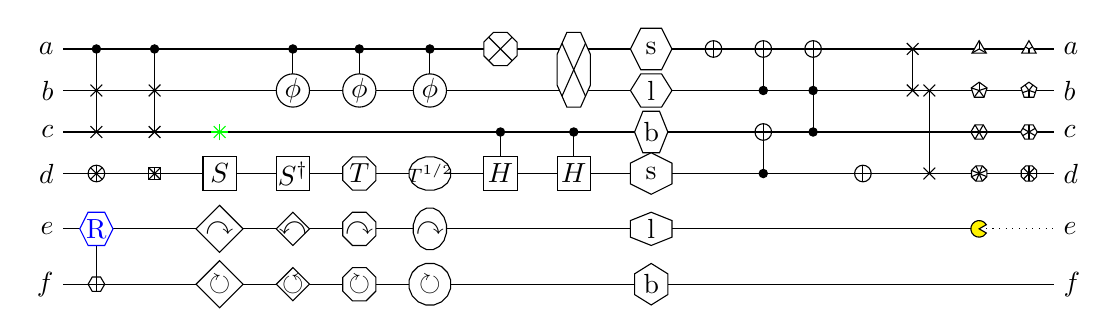
\begin{tikzpicture}[scale=1.000000,x=1pt,y=1pt]
\filldraw[color=white] (0.000000, -7.500000) rectangle (357.970600, 92.500000);
% Drawing wires
% Line 2: a W a a
\draw[color=black] (0.000000,85.000000) -- (357.970600,85.000000);
\draw[color=black] (0.000000,85.000000) node[left] {$a$};
% Line 3: b W b b
\draw[color=black] (0.000000,70.000000) -- (357.970600,70.000000);
\draw[color=black] (0.000000,70.000000) node[left] {$b$};
% Line 4: c W c c
\draw[color=black] (0.000000,55.000000) -- (357.970600,55.000000);
\draw[color=black] (0.000000,55.000000) node[left] {$c$};
% Line 5: d W d d
\draw[color=black] (0.000000,40.000000) -- (357.970600,40.000000);
\draw[color=black] (0.000000,40.000000) node[left] {$d$};
% Line 6: e W e e breadth=25
\draw[color=black] (0.000000,20.000000) -- (330.970600,20.000000);
\draw[color=black,dotted] (330.970600,20.000000) -- (357.970600,20.000000);
\draw[color=black] (0.000000,20.000000) node[left] {$e$};
% Line 7: f W f f
\draw[color=black] (0.000000,0.000000) -- (357.970600,0.000000);
\draw[color=black] (0.000000,0.000000) node[left] {$f$};
% Done with wires; drawing gates
% Line 9: b c SWAP a
\draw (12.000000,85.000000) -- (12.000000,55.000000);
\begin{scope}
\draw (9.878680, 67.878680) -- (14.121320, 72.121320);
\draw (9.878680, 72.121320) -- (14.121320, 67.878680);
\end{scope}
\begin{scope}
\draw (9.878680, 52.878680) -- (14.121320, 57.121320);
\draw (9.878680, 57.121320) -- (14.121320, 52.878680);
\end{scope}
\filldraw (12.000000, 85.000000) circle(1.500000pt);
% Line 12: e G:color=blue R +f shape=6
\draw (12.000000,20.000000) -- (12.000000,0.000000);
\begin{scope}[color=blue]
\begin{scope}
\draw[fill=white] (12.000000, 20.000000) +(-60.000000:6.000000pt and 6.928203pt) -- +(0.000000:6.000000pt and 6.928203pt) -- +(60.000000:6.000000pt and 6.928203pt) -- +(120.000000:6.000000pt and 6.928203pt) -- +(180.000000:6.000000pt and 6.928203pt) -- +(240.000000:6.000000pt and 6.928203pt) -- cycle;
\clip (12.000000, 20.000000) +(-60.000000:6.000000pt and 6.928203pt) -- +(0.000000:6.000000pt and 6.928203pt) -- +(60.000000:6.000000pt and 6.928203pt) -- +(120.000000:6.000000pt and 6.928203pt) -- +(180.000000:6.000000pt and 6.928203pt) -- +(240.000000:6.000000pt and 6.928203pt) -- cycle;
\draw (12.000000, 20.000000) node {R};
\end{scope}
\end{scope}
\begin{scope}
\draw[fill=white] (12.000000, 0.000000) +(-60.000000:3.000000pt) -- +(0.000000:3.000000pt) -- +(60.000000:3.000000pt) -- +(120.000000:3.000000pt) -- +(180.000000:3.000000pt) -- +(240.000000:3.000000pt) -- cycle;
\clip (12.000000, 0.000000) +(-60.000000:3.000000pt) -- +(0.000000:3.000000pt) -- +(60.000000:3.000000pt) -- +(120.000000:3.000000pt) -- +(180.000000:3.000000pt) -- +(240.000000:3.000000pt) -- cycle;
\draw (9.000000, 0.000000) -- (15.000000, 0.000000);
\draw (12.000000, -3.000000) -- (12.000000, 3.000000);
\end{scope}
% Line 13: +d:op=*
\begin{scope}
\draw[fill=white] (12.000000, 40.000000) circle(3.000000pt);
\clip (12.000000, 40.000000) circle(3.000000pt);
\draw (9.000000, 40.000000) -- (15.000000, 40.000000);
\draw (12.000000, 37.000000) -- (12.000000, 43.000000);
\draw (9.878680, 37.878680) -- (14.121320, 42.121320);
\draw (9.878680, 42.121320) -- (14.121320, 37.878680);
\end{scope}
% Line 10: +b +c a op=x:shape=0
\draw (33.000000,85.000000) -- (33.000000,55.000000);
\begin{scope}
\draw (30.878680, 67.878680) -- (35.121320, 72.121320);
\draw (30.878680, 72.121320) -- (35.121320, 67.878680);
\end{scope}
\begin{scope}
\draw (30.878680, 52.878680) -- (35.121320, 57.121320);
\draw (30.878680, 57.121320) -- (35.121320, 52.878680);
\end{scope}
\filldraw (33.000000, 85.000000) circle(1.500000pt);
% Line 14: d:op=*:sh=4
\begin{scope}
\draw[fill=white] (33.000000, 40.000000) +(-45.000000:3.000000pt) -- +(45.000000:3.000000pt) -- +(135.000000:3.000000pt) -- +(225.000000:3.000000pt) -- cycle;
\clip (33.000000, 40.000000) +(-45.000000:3.000000pt) -- +(45.000000:3.000000pt) -- +(135.000000:3.000000pt) -- +(225.000000:3.000000pt) -- cycle;
\draw (30.000000, 40.000000) -- (36.000000, 40.000000);
\draw (33.000000, 37.000000) -- (33.000000, 43.000000);
\draw (30.878680, 37.878680) -- (35.121320, 42.121320);
\draw (30.878680, 42.121320) -- (35.121320, 37.878680);
\end{scope}
% Line 15: c:op=*:sh=0 color=green
\begin{scope}[color=green]
\begin{scope}
\draw (53.500000, 55.000000) -- (59.500000, 55.000000);
\draw (56.500000, 52.000000) -- (56.500000, 58.000000);
\draw (54.378680, 52.878680) -- (58.621320, 57.121320);
\draw (54.378680, 57.121320) -- (58.621320, 52.878680);
\end{scope}
\end{scope}
% Line 17: d G:shape=box $S$
\begin{scope}
\draw[fill=white] (56.500000, 40.000000) +(-45.000000:8.485281pt and 8.485281pt) -- +(45.000000:8.485281pt and 8.485281pt) -- +(135.000000:8.485281pt and 8.485281pt) -- +(225.000000:8.485281pt and 8.485281pt) -- cycle;
\clip (56.500000, 40.000000) +(-45.000000:8.485281pt and 8.485281pt) -- +(45.000000:8.485281pt and 8.485281pt) -- +(135.000000:8.485281pt and 8.485281pt) -- +(225.000000:8.485281pt and 8.485281pt) -- cycle;
\draw (56.500000, 40.000000) node {$S$};
\end{scope}
% Line 18: e:size=17:op=$\curvearrowright$:shape=-4
\begin{scope}
\draw[fill=white] (56.500000, 20.000000) +(-90.000000:8.500000pt) -- +(0.000000:8.500000pt) -- +(90.000000:8.500000pt) -- +(180.000000:8.500000pt) -- cycle;
\clip (56.500000, 20.000000) +(-90.000000:8.500000pt) -- +(0.000000:8.500000pt) -- +(90.000000:8.500000pt) -- +(180.000000:8.500000pt) -- cycle;
\draw (56.500000, 20.000000) node {$\curvearrowright$};
\end{scope}
% Line 19: f:size=17:op=$\circlearrowright$:shape=-4
\begin{scope}
\draw[fill=white] (56.500000, 0.000000) +(-90.000000:8.500000pt) -- +(0.000000:8.500000pt) -- +(90.000000:8.500000pt) -- +(180.000000:8.500000pt) -- cycle;
\clip (56.500000, 0.000000) +(-90.000000:8.500000pt) -- +(0.000000:8.500000pt) -- +(90.000000:8.500000pt) -- +(180.000000:8.500000pt) -- cycle;
\draw (56.500000, 0.000000) node {$\circlearrowright$};
\end{scope}
% Line 22: TOUCH
% Line 23: b P $\phi$ a
\draw (83.000000,85.000000) -- (83.000000,70.000000);
\begin{scope}
\draw[fill=white] (83.000000, 70.000000) circle(6.000000pt);
\clip (83.000000, 70.000000) circle(6.000000pt);
\draw (83.000000, 70.000000) node {$\phi$};
\end{scope}
\filldraw (83.000000, 85.000000) circle(1.500000pt);
% Line 25: d G $S^\dagger$
\begin{scope}
\draw[fill=white] (83.000000, 40.000000) +(-45.000000:8.485281pt and 8.485281pt) -- +(45.000000:8.485281pt and 8.485281pt) -- +(135.000000:8.485281pt and 8.485281pt) -- +(225.000000:8.485281pt and 8.485281pt) -- cycle;
\clip (83.000000, 40.000000) +(-45.000000:8.485281pt and 8.485281pt) -- +(45.000000:8.485281pt and 8.485281pt) -- +(135.000000:8.485281pt and 8.485281pt) -- +(225.000000:8.485281pt and 8.485281pt) -- cycle;
\draw (83.000000, 40.000000) node {$S^\dagger$};
\end{scope}
% Line 26: e G:shape=-4 $\curvearrowleft$
\begin{scope}
\draw[fill=white] (83.000000, 20.000000) +(-90.000000:6.000000pt) -- +(0.000000:6.000000pt) -- +(90.000000:6.000000pt) -- +(180.000000:6.000000pt) -- cycle;
\clip (83.000000, 20.000000) +(-90.000000:6.000000pt) -- +(0.000000:6.000000pt) -- +(90.000000:6.000000pt) -- +(180.000000:6.000000pt) -- cycle;
\draw (83.000000, 20.000000) node {$\curvearrowleft$};
\end{scope}
% Line 27: f G $\circlearrowleft$ shape=-4
\begin{scope}
\draw[fill=white] (83.000000, 0.000000) +(-90.000000:6.000000pt) -- +(0.000000:6.000000pt) -- +(90.000000:6.000000pt) -- +(180.000000:6.000000pt) -- cycle;
\clip (83.000000, 0.000000) +(-90.000000:6.000000pt) -- +(0.000000:6.000000pt) -- +(90.000000:6.000000pt) -- +(180.000000:6.000000pt) -- cycle;
\draw (83.000000, 0.000000) node {$\circlearrowleft$};
\end{scope}
% Line 24: +b a op=$\phi$ size=12
\draw (107.000000,85.000000) -- (107.000000,70.000000);
\begin{scope}
\draw[fill=white] (107.000000, 70.000000) circle(6.000000pt);
\clip (107.000000, 70.000000) circle(6.000000pt);
\draw (107.000000, 70.000000) node {$\phi$};
\end{scope}
\filldraw (107.000000, 85.000000) circle(1.500000pt);
% Line 28: d G:shape=8 $T$
\begin{scope}
\draw[fill=white] (107.000000, 40.000000) +(-67.500000:6.494353pt and 6.494353pt) -- +(-22.500000:6.494353pt and 6.494353pt) -- +(22.500000:6.494353pt and 6.494353pt) -- +(67.500000:6.494353pt and 6.494353pt) -- +(112.500000:6.494353pt and 6.494353pt) -- +(157.500000:6.494353pt and 6.494353pt) -- +(202.500000:6.494353pt and 6.494353pt) -- +(247.500000:6.494353pt and 6.494353pt) -- cycle;
\clip (107.000000, 40.000000) +(-67.500000:6.494353pt and 6.494353pt) -- +(-22.500000:6.494353pt and 6.494353pt) -- +(22.500000:6.494353pt and 6.494353pt) -- +(67.500000:6.494353pt and 6.494353pt) -- +(112.500000:6.494353pt and 6.494353pt) -- +(157.500000:6.494353pt and 6.494353pt) -- +(202.500000:6.494353pt and 6.494353pt) -- +(247.500000:6.494353pt and 6.494353pt) -- cycle;
\draw (107.000000, 40.000000) node {$T$};
\end{scope}
% Line 29: e P $\curvearrowright$ shape=8
\begin{scope}
\draw[fill=white] (107.000000, 20.000000) +(-67.500000:6.494353pt) -- +(-22.500000:6.494353pt) -- +(22.500000:6.494353pt) -- +(67.500000:6.494353pt) -- +(112.500000:6.494353pt) -- +(157.500000:6.494353pt) -- +(202.500000:6.494353pt) -- +(247.500000:6.494353pt) -- cycle;
\clip (107.000000, 20.000000) +(-67.500000:6.494353pt) -- +(-22.500000:6.494353pt) -- +(22.500000:6.494353pt) -- +(67.500000:6.494353pt) -- +(112.500000:6.494353pt) -- +(157.500000:6.494353pt) -- +(202.500000:6.494353pt) -- +(247.500000:6.494353pt) -- cycle;
\draw (107.000000, 20.000000) node {$\curvearrowright$};
\end{scope}
% Line 30: f P $\circlearrowright$ shape=8
\begin{scope}
\draw[fill=white] (107.000000, 0.000000) +(-67.500000:6.494353pt) -- +(-22.500000:6.494353pt) -- +(22.500000:6.494353pt) -- +(67.500000:6.494353pt) -- +(112.500000:6.494353pt) -- +(157.500000:6.494353pt) -- +(202.500000:6.494353pt) -- +(247.500000:6.494353pt) -- cycle;
\clip (107.000000, 0.000000) +(-67.500000:6.494353pt) -- +(-22.500000:6.494353pt) -- +(22.500000:6.494353pt) -- +(67.500000:6.494353pt) -- +(112.500000:6.494353pt) -- +(157.500000:6.494353pt) -- +(202.500000:6.494353pt) -- +(247.500000:6.494353pt) -- cycle;
\draw (107.000000, 0.000000) node {$\circlearrowright$};
\end{scope}
% Line 31: d G $\scriptstyle T^{1/2}$ shape=16 width=15
\begin{scope}
\draw[fill=white] (132.500000, 40.000000) +(-78.750000:7.646934pt and 6.117547pt) -- +(-56.250000:7.646934pt and 6.117547pt) -- +(-33.750000:7.646934pt and 6.117547pt) -- +(-11.250000:7.646934pt and 6.117547pt) -- +(11.250000:7.646934pt and 6.117547pt) -- +(33.750000:7.646934pt and 6.117547pt) -- +(56.250000:7.646934pt and 6.117547pt) -- +(78.750000:7.646934pt and 6.117547pt) -- +(101.250000:7.646934pt and 6.117547pt) -- +(123.750000:7.646934pt and 6.117547pt) -- +(146.250000:7.646934pt and 6.117547pt) -- +(168.750000:7.646934pt and 6.117547pt) -- +(191.250000:7.646934pt and 6.117547pt) -- +(213.750000:7.646934pt and 6.117547pt) -- +(236.250000:7.646934pt and 6.117547pt) -- +(258.750000:7.646934pt and 6.117547pt) -- cycle;
\clip (132.500000, 40.000000) +(-78.750000:7.646934pt and 6.117547pt) -- +(-56.250000:7.646934pt and 6.117547pt) -- +(-33.750000:7.646934pt and 6.117547pt) -- +(-11.250000:7.646934pt and 6.117547pt) -- +(11.250000:7.646934pt and 6.117547pt) -- +(33.750000:7.646934pt and 6.117547pt) -- +(56.250000:7.646934pt and 6.117547pt) -- +(78.750000:7.646934pt and 6.117547pt) -- +(101.250000:7.646934pt and 6.117547pt) -- +(123.750000:7.646934pt and 6.117547pt) -- +(146.250000:7.646934pt and 6.117547pt) -- +(168.750000:7.646934pt and 6.117547pt) -- +(191.250000:7.646934pt and 6.117547pt) -- +(213.750000:7.646934pt and 6.117547pt) -- +(236.250000:7.646934pt and 6.117547pt) -- +(258.750000:7.646934pt and 6.117547pt) -- cycle;
\draw (132.500000, 40.000000) node {$\scriptstyle T^{1/2}$};
\end{scope}
% Line 32: e G $\curvearrowright$ shape=16 height=15
\begin{scope}
\draw[fill=white] (132.500000, 20.000000) +(-78.750000:6.117547pt and 7.646934pt) -- +(-56.250000:6.117547pt and 7.646934pt) -- +(-33.750000:6.117547pt and 7.646934pt) -- +(-11.250000:6.117547pt and 7.646934pt) -- +(11.250000:6.117547pt and 7.646934pt) -- +(33.750000:6.117547pt and 7.646934pt) -- +(56.250000:6.117547pt and 7.646934pt) -- +(78.750000:6.117547pt and 7.646934pt) -- +(101.250000:6.117547pt and 7.646934pt) -- +(123.750000:6.117547pt and 7.646934pt) -- +(146.250000:6.117547pt and 7.646934pt) -- +(168.750000:6.117547pt and 7.646934pt) -- +(191.250000:6.117547pt and 7.646934pt) -- +(213.750000:6.117547pt and 7.646934pt) -- +(236.250000:6.117547pt and 7.646934pt) -- +(258.750000:6.117547pt and 7.646934pt) -- cycle;
\clip (132.500000, 20.000000) +(-78.750000:6.117547pt and 7.646934pt) -- +(-56.250000:6.117547pt and 7.646934pt) -- +(-33.750000:6.117547pt and 7.646934pt) -- +(-11.250000:6.117547pt and 7.646934pt) -- +(11.250000:6.117547pt and 7.646934pt) -- +(33.750000:6.117547pt and 7.646934pt) -- +(56.250000:6.117547pt and 7.646934pt) -- +(78.750000:6.117547pt and 7.646934pt) -- +(101.250000:6.117547pt and 7.646934pt) -- +(123.750000:6.117547pt and 7.646934pt) -- +(146.250000:6.117547pt and 7.646934pt) -- +(168.750000:6.117547pt and 7.646934pt) -- +(191.250000:6.117547pt and 7.646934pt) -- +(213.750000:6.117547pt and 7.646934pt) -- +(236.250000:6.117547pt and 7.646934pt) -- +(258.750000:6.117547pt and 7.646934pt) -- cycle;
\draw (132.500000, 20.000000) node {$\curvearrowright$};
\end{scope}
% Line 33: f G $\circlearrowright$ shape=16 size=15
\begin{scope}
\draw[fill=white] (132.500000, -0.000000) +(-78.750000:7.646934pt) -- +(-56.250000:7.646934pt) -- +(-33.750000:7.646934pt) -- +(-11.250000:7.646934pt) -- +(11.250000:7.646934pt) -- +(33.750000:7.646934pt) -- +(56.250000:7.646934pt) -- +(78.750000:7.646934pt) -- +(101.250000:7.646934pt) -- +(123.750000:7.646934pt) -- +(146.250000:7.646934pt) -- +(168.750000:7.646934pt) -- +(191.250000:7.646934pt) -- +(213.750000:7.646934pt) -- +(236.250000:7.646934pt) -- +(258.750000:7.646934pt) -- cycle;
\clip (132.500000, -0.000000) +(-78.750000:7.646934pt) -- +(-56.250000:7.646934pt) -- +(-33.750000:7.646934pt) -- +(-11.250000:7.646934pt) -- +(11.250000:7.646934pt) -- +(33.750000:7.646934pt) -- +(56.250000:7.646934pt) -- +(78.750000:7.646934pt) -- +(101.250000:7.646934pt) -- +(123.750000:7.646934pt) -- +(146.250000:7.646934pt) -- +(168.750000:7.646934pt) -- +(191.250000:7.646934pt) -- +(213.750000:7.646934pt) -- +(236.250000:7.646934pt) -- +(258.750000:7.646934pt) -- cycle;
\draw (132.500000, -0.000000) node {$\circlearrowright$};
\end{scope}
% Line 35: +b:size=12 a op=$\phi$
\draw (132.500000,85.000000) -- (132.500000,70.000000);
\begin{scope}
\draw[fill=white] (132.500000, 70.000000) circle(6.000000pt);
\clip (132.500000, 70.000000) circle(6.000000pt);
\draw (132.500000, 70.000000) node {$\phi$};
\end{scope}
\filldraw (132.500000, 85.000000) circle(1.500000pt);
% Line 37: a G x shape=8
\begin{scope}
\draw[fill=white] (158.000000, 85.000000) +(-67.500000:6.494353pt and 6.494353pt) -- +(-22.500000:6.494353pt and 6.494353pt) -- +(22.500000:6.494353pt and 6.494353pt) -- +(67.500000:6.494353pt and 6.494353pt) -- +(112.500000:6.494353pt and 6.494353pt) -- +(157.500000:6.494353pt and 6.494353pt) -- +(202.500000:6.494353pt and 6.494353pt) -- +(247.500000:6.494353pt and 6.494353pt) -- cycle;
\clip (158.000000, 85.000000) +(-67.500000:6.494353pt and 6.494353pt) -- +(-22.500000:6.494353pt and 6.494353pt) -- +(22.500000:6.494353pt and 6.494353pt) -- +(67.500000:6.494353pt and 6.494353pt) -- +(112.500000:6.494353pt and 6.494353pt) -- +(157.500000:6.494353pt and 6.494353pt) -- +(202.500000:6.494353pt and 6.494353pt) -- +(247.500000:6.494353pt and 6.494353pt) -- cycle;
\draw (153.407799, 80.407799) -- (162.592201, 89.592201);
\draw (153.407799, 89.592201) -- (162.592201, 80.407799);
\end{scope}
% Line 40: d H c
\draw (158.000000,55.000000) -- (158.000000,40.000000);
\begin{scope}
\draw[fill=white] (158.000000, 40.000000) +(-45.000000:8.485281pt and 8.485281pt) -- +(45.000000:8.485281pt and 8.485281pt) -- +(135.000000:8.485281pt and 8.485281pt) -- +(225.000000:8.485281pt and 8.485281pt) -- cycle;
\clip (158.000000, 40.000000) +(-45.000000:8.485281pt and 8.485281pt) -- +(45.000000:8.485281pt and 8.485281pt) -- +(135.000000:8.485281pt and 8.485281pt) -- +(225.000000:8.485281pt and 8.485281pt) -- cycle;
\draw (158.000000, 40.000000) node {$H$};
\end{scope}
\filldraw (158.000000, 55.000000) circle(1.500000pt);
% Line 38: a b G x shape=8
\draw (184.485300,85.000000) -- (184.485300,70.000000);
\begin{scope}
\draw[fill=white] (184.485300, 77.500000) +(-67.500000:6.494353pt and 14.612295pt) -- +(-22.500000:6.494353pt and 14.612295pt) -- +(22.500000:6.494353pt and 14.612295pt) -- +(67.500000:6.494353pt and 14.612295pt) -- +(112.500000:6.494353pt and 14.612295pt) -- +(157.500000:6.494353pt and 14.612295pt) -- +(202.500000:6.494353pt and 14.612295pt) -- +(247.500000:6.494353pt and 14.612295pt) -- cycle;
\clip (184.485300, 77.500000) +(-67.500000:6.494353pt and 14.612295pt) -- +(-22.500000:6.494353pt and 14.612295pt) -- +(22.500000:6.494353pt and 14.612295pt) -- +(67.500000:6.494353pt and 14.612295pt) -- +(112.500000:6.494353pt and 14.612295pt) -- +(157.500000:6.494353pt and 14.612295pt) -- +(202.500000:6.494353pt and 14.612295pt) -- +(247.500000:6.494353pt and 14.612295pt) -- cycle;
\draw (179.893099, 67.167547) -- (189.077501, 87.832453);
\draw (179.893099, 87.832453) -- (189.077501, 67.167547);
\end{scope}
% Line 41: d:size=16.9706:op=$H$:shape=box c
\draw (184.485300,55.000000) -- (184.485300,40.000000);
\begin{scope}
\draw[fill=white] (184.485300, 40.000000) +(-45.000000:8.485300pt) -- +(45.000000:8.485300pt) -- +(135.000000:8.485300pt) -- +(225.000000:8.485300pt) -- cycle;
\clip (184.485300, 40.000000) +(-45.000000:8.485300pt) -- +(45.000000:8.485300pt) -- +(135.000000:8.485300pt) -- +(225.000000:8.485300pt) -- cycle;
\draw (184.485300, 40.000000) node {$H$};
\end{scope}
\filldraw (184.485300, 55.000000) circle(1.500000pt);
% Line 44: a G:sh=6 s size=15
\begin{scope}
\draw[fill=white] (212.470600, 85.000000) +(-60.000000:7.500000pt and 8.660254pt) -- +(0.000000:7.500000pt and 8.660254pt) -- +(60.000000:7.500000pt and 8.660254pt) -- +(120.000000:7.500000pt and 8.660254pt) -- +(180.000000:7.500000pt and 8.660254pt) -- +(240.000000:7.500000pt and 8.660254pt) -- cycle;
\clip (212.470600, 85.000000) +(-60.000000:7.500000pt and 8.660254pt) -- +(0.000000:7.500000pt and 8.660254pt) -- +(60.000000:7.500000pt and 8.660254pt) -- +(120.000000:7.500000pt and 8.660254pt) -- +(180.000000:7.500000pt and 8.660254pt) -- +(240.000000:7.500000pt and 8.660254pt) -- cycle;
\draw (212.470600, 85.000000) node {s};
\end{scope}
% Line 45: b G:sh=6 l length=15
\begin{scope}
\draw[fill=white] (212.470600, 70.000000) +(-60.000000:7.500000pt and 6.928203pt) -- +(0.000000:7.500000pt and 6.928203pt) -- +(60.000000:7.500000pt and 6.928203pt) -- +(120.000000:7.500000pt and 6.928203pt) -- +(180.000000:7.500000pt and 6.928203pt) -- +(240.000000:7.500000pt and 6.928203pt) -- cycle;
\clip (212.470600, 70.000000) +(-60.000000:7.500000pt and 6.928203pt) -- +(0.000000:7.500000pt and 6.928203pt) -- +(60.000000:7.500000pt and 6.928203pt) -- +(120.000000:7.500000pt and 6.928203pt) -- +(180.000000:7.500000pt and 6.928203pt) -- +(240.000000:7.500000pt and 6.928203pt) -- cycle;
\draw (212.470600, 70.000000) node {l};
\end{scope}
% Line 46: c G:sh=6 b breadth=15
\begin{scope}
\draw[fill=white] (212.470600, 55.000000) +(-60.000000:6.000000pt and 8.660254pt) -- +(0.000000:6.000000pt and 8.660254pt) -- +(60.000000:6.000000pt and 8.660254pt) -- +(120.000000:6.000000pt and 8.660254pt) -- +(180.000000:6.000000pt and 8.660254pt) -- +(240.000000:6.000000pt and 8.660254pt) -- cycle;
\clip (212.470600, 55.000000) +(-60.000000:6.000000pt and 8.660254pt) -- +(0.000000:6.000000pt and 8.660254pt) -- +(60.000000:6.000000pt and 8.660254pt) -- +(120.000000:6.000000pt and 8.660254pt) -- +(180.000000:6.000000pt and 8.660254pt) -- +(240.000000:6.000000pt and 8.660254pt) -- cycle;
\draw (212.470600, 55.000000) node {b};
\end{scope}
% Line 47: d G:sh=-6 s size=15
\begin{scope}
\draw[fill=white] (212.470600, 40.000000) +(-90.000000:8.660254pt and 7.500000pt) -- +(-30.000000:8.660254pt and 7.500000pt) -- +(30.000000:8.660254pt and 7.500000pt) -- +(90.000000:8.660254pt and 7.500000pt) -- +(150.000000:8.660254pt and 7.500000pt) -- +(210.000000:8.660254pt and 7.500000pt) -- cycle;
\clip (212.470600, 40.000000) +(-90.000000:8.660254pt and 7.500000pt) -- +(-30.000000:8.660254pt and 7.500000pt) -- +(30.000000:8.660254pt and 7.500000pt) -- +(90.000000:8.660254pt and 7.500000pt) -- +(150.000000:8.660254pt and 7.500000pt) -- +(210.000000:8.660254pt and 7.500000pt) -- cycle;
\draw (212.470600, 40.000000) node {s};
\end{scope}
% Line 48: e G:sh=-6 l length=15
\begin{scope}
\draw[fill=white] (212.470600, 20.000000) +(-90.000000:8.660254pt and 6.000000pt) -- +(-30.000000:8.660254pt and 6.000000pt) -- +(30.000000:8.660254pt and 6.000000pt) -- +(90.000000:8.660254pt and 6.000000pt) -- +(150.000000:8.660254pt and 6.000000pt) -- +(210.000000:8.660254pt and 6.000000pt) -- cycle;
\clip (212.470600, 20.000000) +(-90.000000:8.660254pt and 6.000000pt) -- +(-30.000000:8.660254pt and 6.000000pt) -- +(30.000000:8.660254pt and 6.000000pt) -- +(90.000000:8.660254pt and 6.000000pt) -- +(150.000000:8.660254pt and 6.000000pt) -- +(210.000000:8.660254pt and 6.000000pt) -- cycle;
\draw (212.470600, 20.000000) node {l};
\end{scope}
% Line 49: f G:sh=-6 b breadth=15
\begin{scope}
\draw[fill=white] (212.470600, 0.000000) +(-90.000000:6.928203pt and 7.500000pt) -- +(-30.000000:6.928203pt and 7.500000pt) -- +(30.000000:6.928203pt and 7.500000pt) -- +(90.000000:6.928203pt and 7.500000pt) -- +(150.000000:6.928203pt and 7.500000pt) -- +(210.000000:6.928203pt and 7.500000pt) -- cycle;
\clip (212.470600, 0.000000) +(-90.000000:6.928203pt and 7.500000pt) -- +(-30.000000:6.928203pt and 7.500000pt) -- +(30.000000:6.928203pt and 7.500000pt) -- +(90.000000:6.928203pt and 7.500000pt) -- +(150.000000:6.928203pt and 7.500000pt) -- +(210.000000:6.928203pt and 7.500000pt) -- cycle;
\draw (212.470600, 0.000000) node {b};
\end{scope}
% Line 52: TOUCH
% Line 55: +a
\begin{scope}
\draw[fill=white] (234.970600, 85.000000) circle(3.000000pt);
\clip (234.970600, 85.000000) circle(3.000000pt);
\draw (231.970600, 85.000000) -- (237.970600, 85.000000);
\draw (234.970600, 82.000000) -- (234.970600, 88.000000);
\end{scope}
% Line 56: +a b
\draw (252.970600,85.000000) -- (252.970600,70.000000);
\begin{scope}
\draw[fill=white] (252.970600, 85.000000) circle(3.000000pt);
\clip (252.970600, 85.000000) circle(3.000000pt);
\draw (249.970600, 85.000000) -- (255.970600, 85.000000);
\draw (252.970600, 82.000000) -- (252.970600, 88.000000);
\end{scope}
\filldraw (252.970600, 70.000000) circle(1.500000pt);
% Line 57: +c d
\draw (252.970600,55.000000) -- (252.970600,40.000000);
\begin{scope}
\draw[fill=white] (252.970600, 55.000000) circle(3.000000pt);
\clip (252.970600, 55.000000) circle(3.000000pt);
\draw (249.970600, 55.000000) -- (255.970600, 55.000000);
\draw (252.970600, 52.000000) -- (252.970600, 58.000000);
\end{scope}
\filldraw (252.970600, 40.000000) circle(1.500000pt);
% Line 59: +a b c
\draw (270.970600,85.000000) -- (270.970600,55.000000);
\begin{scope}
\draw[fill=white] (270.970600, 85.000000) circle(3.000000pt);
\clip (270.970600, 85.000000) circle(3.000000pt);
\draw (267.970600, 85.000000) -- (273.970600, 85.000000);
\draw (270.970600, 82.000000) -- (270.970600, 88.000000);
\end{scope}
\filldraw (270.970600, 70.000000) circle(1.500000pt);
\filldraw (270.970600, 55.000000) circle(1.500000pt);
% Line 60: +d
\begin{scope}
\draw[fill=white] (288.970600, 40.000000) circle(3.000000pt);
\clip (288.970600, 40.000000) circle(3.000000pt);
\draw (285.970600, 40.000000) -- (291.970600, 40.000000);
\draw (288.970600, 37.000000) -- (288.970600, 43.000000);
\end{scope}
% Line 63: a b SWAP
\draw (306.970600,85.000000) -- (306.970600,70.000000);
\begin{scope}
\draw (304.849280, 82.878680) -- (309.091920, 87.121320);
\draw (304.849280, 87.121320) -- (309.091920, 82.878680);
\end{scope}
\begin{scope}
\draw (304.849280, 67.878680) -- (309.091920, 72.121320);
\draw (304.849280, 72.121320) -- (309.091920, 67.878680);
\end{scope}
% Line 64: +b +d op=x:shape=0
\draw (312.970600,70.000000) -- (312.970600,40.000000);
\begin{scope}
\draw (310.849280, 67.878680) -- (315.091920, 72.121320);
\draw (310.849280, 72.121320) -- (315.091920, 67.878680);
\end{scope}
\begin{scope}
\draw (310.849280, 37.878680) -- (315.091920, 42.121320);
\draw (310.849280, 42.121320) -- (315.091920, 37.878680);
\end{scope}
% Line 67: TOUCH
% Line 68: a:op=*:sh=3
\begin{scope}
\draw[fill=white] (330.970600, 85.000000) +(-30.000000:3.000000pt) -- +(90.000000:3.000000pt) -- +(210.000000:3.000000pt) -- cycle;
\clip (330.970600, 85.000000) +(-30.000000:3.000000pt) -- +(90.000000:3.000000pt) -- +(210.000000:3.000000pt) -- cycle;
\draw (330.970600, 85.000000) -- +(-30.000000:3.000000pt);
\draw (330.970600, 85.000000) -- +(90.000000:3.000000pt);
\draw (330.970600, 85.000000) -- +(210.000000:3.000000pt);
\end{scope}
% Line 69: b:op=*:sh=5
\begin{scope}
\draw[fill=white] (330.970600, 70.000000) +(-54.000000:3.000000pt) -- +(18.000000:3.000000pt) -- +(90.000000:3.000000pt) -- +(162.000000:3.000000pt) -- +(234.000000:3.000000pt) -- cycle;
\clip (330.970600, 70.000000) +(-54.000000:3.000000pt) -- +(18.000000:3.000000pt) -- +(90.000000:3.000000pt) -- +(162.000000:3.000000pt) -- +(234.000000:3.000000pt) -- cycle;
\draw (330.970600, 70.000000) -- +(-54.000000:3.000000pt);
\draw (330.970600, 70.000000) -- +(18.000000:3.000000pt);
\draw (330.970600, 70.000000) -- +(90.000000:3.000000pt);
\draw (330.970600, 70.000000) -- +(162.000000:3.000000pt);
\draw (330.970600, 70.000000) -- +(234.000000:3.000000pt);
\end{scope}
% Line 70: c:op=*:sh=6
\begin{scope}
\draw[fill=white] (330.970600, 55.000000) +(-60.000000:3.000000pt) -- +(0.000000:3.000000pt) -- +(60.000000:3.000000pt) -- +(120.000000:3.000000pt) -- +(180.000000:3.000000pt) -- +(240.000000:3.000000pt) -- cycle;
\clip (330.970600, 55.000000) +(-60.000000:3.000000pt) -- +(0.000000:3.000000pt) -- +(60.000000:3.000000pt) -- +(120.000000:3.000000pt) -- +(180.000000:3.000000pt) -- +(240.000000:3.000000pt) -- cycle;
\draw (330.970600, 55.000000) -- +(-60.000000:3.000000pt);
\draw (330.970600, 55.000000) -- +(0.000000:3.000000pt);
\draw (330.970600, 55.000000) -- +(60.000000:3.000000pt);
\draw (330.970600, 55.000000) -- +(120.000000:3.000000pt);
\draw (330.970600, 55.000000) -- +(180.000000:3.000000pt);
\draw (330.970600, 55.000000) -- +(240.000000:3.000000pt);
\end{scope}
% Line 71: d:op=*:sh=8
\begin{scope}
\draw[fill=white] (330.970600, 40.000000) +(-67.500000:3.000000pt) -- +(-22.500000:3.000000pt) -- +(22.500000:3.000000pt) -- +(67.500000:3.000000pt) -- +(112.500000:3.000000pt) -- +(157.500000:3.000000pt) -- +(202.500000:3.000000pt) -- +(247.500000:3.000000pt) -- cycle;
\clip (330.970600, 40.000000) +(-67.500000:3.000000pt) -- +(-22.500000:3.000000pt) -- +(22.500000:3.000000pt) -- +(67.500000:3.000000pt) -- +(112.500000:3.000000pt) -- +(157.500000:3.000000pt) -- +(202.500000:3.000000pt) -- +(247.500000:3.000000pt) -- cycle;
\draw (330.970600, 40.000000) -- +(-67.500000:3.000000pt);
\draw (330.970600, 40.000000) -- +(-22.500000:3.000000pt);
\draw (330.970600, 40.000000) -- +(22.500000:3.000000pt);
\draw (330.970600, 40.000000) -- +(67.500000:3.000000pt);
\draw (330.970600, 40.000000) -- +(112.500000:3.000000pt);
\draw (330.970600, 40.000000) -- +(157.500000:3.000000pt);
\draw (330.970600, 40.000000) -- +(202.500000:3.000000pt);
\draw (330.970600, 40.000000) -- +(247.500000:3.000000pt);
\end{scope}
% Line 78: e:op="\draw[fill=yellow] (0,0) -- (30:3pt) arc (30:330:3pt) -- cycle;":sh=0:style=dotted
\begin{scope}
\begin{scope}[shift={(330.970600,20.000000)}]
\draw[fill=yellow] (0,0) -- (30:3pt) arc (30:330:3pt) -- cycle;
\end{scope}
\end{scope}
% Line 73: a:op=-*:sh=3
\begin{scope}
\draw[fill=white] (348.970600, 85.000000) +(-30.000000:3.000000pt) -- +(90.000000:3.000000pt) -- +(210.000000:3.000000pt) -- cycle;
\clip (348.970600, 85.000000) +(-30.000000:3.000000pt) -- +(90.000000:3.000000pt) -- +(210.000000:3.000000pt) -- cycle;
\draw (348.970600, 85.000000) -- +(30.000000:3.000000pt);
\draw (348.970600, 85.000000) -- +(150.000000:3.000000pt);
\draw (348.970600, 85.000000) -- +(270.000000:3.000000pt);
\end{scope}
% Line 74: b:op=-*:sh=5
\begin{scope}
\draw[fill=white] (348.970600, 70.000000) +(-54.000000:3.000000pt) -- +(18.000000:3.000000pt) -- +(90.000000:3.000000pt) -- +(162.000000:3.000000pt) -- +(234.000000:3.000000pt) -- cycle;
\clip (348.970600, 70.000000) +(-54.000000:3.000000pt) -- +(18.000000:3.000000pt) -- +(90.000000:3.000000pt) -- +(162.000000:3.000000pt) -- +(234.000000:3.000000pt) -- cycle;
\draw (348.970600, 70.000000) -- +(-18.000000:3.000000pt);
\draw (348.970600, 70.000000) -- +(54.000000:3.000000pt);
\draw (348.970600, 70.000000) -- +(126.000000:3.000000pt);
\draw (348.970600, 70.000000) -- +(198.000000:3.000000pt);
\draw (348.970600, 70.000000) -- +(270.000000:3.000000pt);
\end{scope}
% Line 75: c:op=-*:sh=6
\begin{scope}
\draw[fill=white] (348.970600, 55.000000) +(-60.000000:3.000000pt) -- +(0.000000:3.000000pt) -- +(60.000000:3.000000pt) -- +(120.000000:3.000000pt) -- +(180.000000:3.000000pt) -- +(240.000000:3.000000pt) -- cycle;
\clip (348.970600, 55.000000) +(-60.000000:3.000000pt) -- +(0.000000:3.000000pt) -- +(60.000000:3.000000pt) -- +(120.000000:3.000000pt) -- +(180.000000:3.000000pt) -- +(240.000000:3.000000pt) -- cycle;
\draw (348.970600, 55.000000) -- +(-30.000000:3.000000pt);
\draw (348.970600, 55.000000) -- +(30.000000:3.000000pt);
\draw (348.970600, 55.000000) -- +(90.000000:3.000000pt);
\draw (348.970600, 55.000000) -- +(150.000000:3.000000pt);
\draw (348.970600, 55.000000) -- +(210.000000:3.000000pt);
\draw (348.970600, 55.000000) -- +(270.000000:3.000000pt);
\end{scope}
% Line 76: d:op=-*:sh=8
\begin{scope}
\draw[fill=white] (348.970600, 40.000000) +(-67.500000:3.000000pt) -- +(-22.500000:3.000000pt) -- +(22.500000:3.000000pt) -- +(67.500000:3.000000pt) -- +(112.500000:3.000000pt) -- +(157.500000:3.000000pt) -- +(202.500000:3.000000pt) -- +(247.500000:3.000000pt) -- cycle;
\clip (348.970600, 40.000000) +(-67.500000:3.000000pt) -- +(-22.500000:3.000000pt) -- +(22.500000:3.000000pt) -- +(67.500000:3.000000pt) -- +(112.500000:3.000000pt) -- +(157.500000:3.000000pt) -- +(202.500000:3.000000pt) -- +(247.500000:3.000000pt) -- cycle;
\draw (348.970600, 40.000000) -- +(-45.000000:3.000000pt);
\draw (348.970600, 40.000000) -- +(0.000000:3.000000pt);
\draw (348.970600, 40.000000) -- +(45.000000:3.000000pt);
\draw (348.970600, 40.000000) -- +(90.000000:3.000000pt);
\draw (348.970600, 40.000000) -- +(135.000000:3.000000pt);
\draw (348.970600, 40.000000) -- +(180.000000:3.000000pt);
\draw (348.970600, 40.000000) -- +(225.000000:3.000000pt);
\draw (348.970600, 40.000000) -- +(270.000000:3.000000pt);
\end{scope}
% Done with gates; drawing ending labels
\draw[color=black] (357.970600,85.000000) node[right] {$a$};
\draw[color=black] (357.970600,70.000000) node[right] {$b$};
\draw[color=black] (357.970600,55.000000) node[right] {$c$};
\draw[color=black] (357.970600,40.000000) node[right] {$d$};
\draw[color=black] (357.970600,20.000000) node[right] {$e$};
\draw[color=black] (357.970600,0.000000) node[right] {$f$};
% Done with ending labels; drawing cut lines and comments
% Done with comments
\end{tikzpicture}

\end{figure}

\SaveVerb{name}|measure|
\begin{figure}[ht]
\caption{\protect\UseVerb{name}}
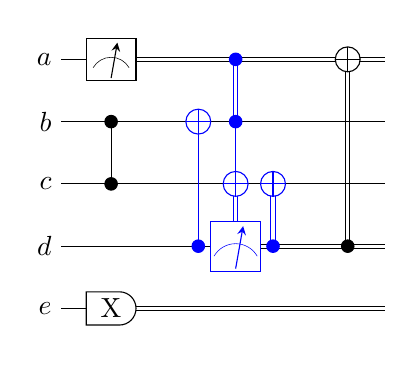
\begin{tikzpicture}[scale=1.500000,x=1pt,y=1pt]
\filldraw[color=white] (0.000000, -7.500000) rectangle (78.000000, 67.500000);
% Drawing wires
% Line 3: a W a
\draw[color=black] (0.000000,60.000000) -- (12.000000,60.000000);
\draw[color=black] (12.000000,59.500000) -- (78.000000,59.500000);
\draw[color=black] (12.000000,60.500000) -- (78.000000,60.500000);
\draw[color=black] (0.000000,60.000000) node[left] {$a$};
% Line 4: b W b
\draw[color=black] (0.000000,45.000000) -- (78.000000,45.000000);
\draw[color=black] (0.000000,45.000000) node[left] {$b$};
% Line 5: c W c
\draw[color=black] (0.000000,30.000000) -- (78.000000,30.000000);
\draw[color=black] (0.000000,30.000000) node[left] {$c$};
% Line 6: d W d
\draw[color=black] (0.000000,15.000000) -- (42.000000,15.000000);
\draw[color=black] (42.000000,14.500000) -- (78.000000,14.500000);
\draw[color=black] (42.000000,15.500000) -- (78.000000,15.500000);
\draw[color=black] (0.000000,15.000000) node[left] {$d$};
% Line 7: ee W e
\draw[color=black] (0.000000,0.000000) -- (12.000000,0.000000);
\draw[color=black] (12.000000,-0.500000) -- (78.000000,-0.500000);
\draw[color=black] (12.000000,0.500000) -- (78.000000,0.500000);
\draw[color=black] (0.000000,0.000000) node[left] {$e$};
% Done with wires; drawing gates
% Line 9: a M breadth=10
\draw[fill=white] (6.000000, 55.000000) rectangle (18.000000, 65.000000);
\draw[very thin] (12.000000, 60.500000) arc (90:150:5.000000pt);
\draw[very thin] (12.000000, 60.500000) arc (90:30:5.000000pt);
\draw[->,>=stealth] (12.000000, 55.500000) -- +(80:8.660254pt);
% Line 10: b c
\draw (12.000000,45.000000) -- (12.000000,30.000000);
\filldraw (12.000000, 45.000000) circle(1.500000pt);
\filldraw (12.000000, 30.000000) circle(1.500000pt);
% Line 17: ee M X
\draw[fill=white] (6.000000, -4.000000) -- (14.000000,-4.000000) arc (-90:90:4.000000pt) -- (6.000000,4.000000) -- cycle;
\draw (12.000000, 0.000000) node {X};
% Line 12: +b d
\begin{scope}[color=blue]
\draw (33.000000,45.000000) -- (33.000000,15.000000);
\begin{scope}
\draw[fill=white] (33.000000, 45.000000) circle(3.000000pt);
\clip (33.000000, 45.000000) circle(3.000000pt);
\draw (30.000000, 45.000000) -- (36.000000, 45.000000);
\draw (33.000000, 42.000000) -- (33.000000, 48.000000);
\end{scope}
\filldraw (33.000000, 15.000000) circle(1.500000pt);
\end{scope}
% Line 13: +c a b d:type=c
\begin{scope}[color=blue]
\draw (41.500000,60.000000) -- (41.500000,45.000000);
\draw (42.500000,60.000000) -- (42.500000,45.000000);
\draw (42.000000,45.000000) -- (42.000000,30.000000);
\draw (41.500000,30.000000) -- (41.500000,15.000000);
\draw (42.500000,30.000000) -- (42.500000,15.000000);
\begin{scope}
\draw[fill=white] (42.000000, 30.000000) circle(3.000000pt);
\clip (42.000000, 30.000000) circle(3.000000pt);
\draw (39.000000, 30.000000) -- (45.000000, 30.000000);
\draw (42.000000, 27.000000) -- (42.000000, 33.000000);
\end{scope}
\filldraw (42.000000, 60.000000) circle(1.500000pt);
\filldraw (42.000000, 45.000000) circle(1.500000pt);
\filldraw (42.000000, 15.000000) circle(1.500000pt);
\draw[fill=white] (36.000000, 9.000000) rectangle (48.000000, 21.000000);
\draw[very thin] (42.000000, 15.600000) arc (90:150:6.000000pt);
\draw[very thin] (42.000000, 15.600000) arc (90:30:6.000000pt);
\draw[->,>=stealth] (42.000000, 9.600000) -- +(80:10.392305pt);
\end{scope}
% Line 14: +c d
\begin{scope}[color=blue]
\draw (50.500000,30.000000) -- (50.500000,15.000000);
\draw (51.500000,30.000000) -- (51.500000,15.000000);
\begin{scope}
\draw[fill=white] (51.000000, 30.000000) circle(3.000000pt);
\clip (51.000000, 30.000000) circle(3.000000pt);
\draw (48.000000, 30.000000) -- (54.000000, 30.000000);
\draw (51.000000, 27.000000) -- (51.000000, 33.000000);
\end{scope}
\filldraw (51.000000, 15.000000) circle(1.500000pt);
\end{scope}
% Line 16: +a d
\draw (68.500000,60.000000) -- (68.500000,15.000000);
\draw (69.500000,60.000000) -- (69.500000,15.000000);
\begin{scope}
\draw[fill=white] (69.000000, 60.000000) circle(3.000000pt);
\clip (69.000000, 60.000000) circle(3.000000pt);
\draw (66.000000, 60.000000) -- (72.000000, 60.000000);
\draw (69.000000, 57.000000) -- (69.000000, 63.000000);
\end{scope}
\filldraw (69.000000, 15.000000) circle(1.500000pt);
% Done with gates; drawing ending labels
% Done with ending labels; drawing cut lines and comments
% Done with comments
\end{tikzpicture}

\end{figure}

\SaveVerb{name}|measure_tag|
\begin{figure}[ht]
\caption{\protect\UseVerb{name}}
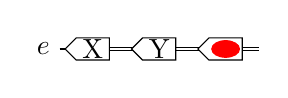
\begin{tikzpicture}[scale=1.000000,x=1pt,y=1pt]
\filldraw[color=white] (0.000000, -7.500000) rectangle (72.000000, 7.500000);
% Drawing wires
% Line 1: ee W e
\draw[color=black] (0.000000,0.000000) -- (12.000000,0.000000);
\draw[color=black] (12.000000,-0.500000) -- (36.000000,-0.500000);
\draw[color=black] (12.000000,0.500000) -- (36.000000,0.500000);
\draw[color=black] (36.000000,-0.500000) -- (60.000000,-0.500000);
\draw[color=black] (36.000000,0.500000) -- (60.000000,0.500000);
\draw[color=black] (60.000000,-0.500000) -- (72.000000,-0.500000);
\draw[color=black] (60.000000,0.500000) -- (72.000000,0.500000);
\draw[color=black] (0.000000,0.000000) node[left] {$e$};
% Done with wires; drawing gates
% Line 4: ee M X
\draw[fill=white] (2.000000, 0.000000) -- (6.000000,4.000000) -- (18.000000,4.000000) -- (18.000000, -4.000000) -- (6.000000, -4.000000) -- cycle;
\draw (12.000000, 0.000000) node {X};
% Line 5: ee M Y
\draw[fill=white] (26.000000, 0.000000) -- (30.000000,4.000000) -- (42.000000,4.000000) -- (42.000000, -4.000000) -- (30.000000, -4.000000) -- cycle;
\draw (36.000000, 0.000000) node {Y};
% Line 6: ee M "\filldraw[color=red] (0,0) ellipse(5pt and 3pt);"
\draw[fill=white] (50.000000, 0.000000) -- (54.000000,4.000000) -- (66.000000,4.000000) -- (66.000000, -4.000000) -- (54.000000, -4.000000) -- cycle;
\begin{scope}[shift={(60.000000,0.000000)}]
\filldraw[color=red] (0,0) ellipse(5pt and 3pt);
\end{scope}
% Done with gates; drawing ending labels
% Done with ending labels; drawing cut lines and comments
% Done with comments
\end{tikzpicture}

\end{figure}

\SaveVerb{name}|oop|
\begin{figure}[ht]
\caption{\protect\UseVerb{name}}
\definecolor{darkgreen}{rgb}{0,.5,0}
\begin{tikzpicture}[scale=1.000000,x=1pt,y=1pt]
\filldraw[color=white] (0.000000, -8.250000) rectangle (273.000000, 585.750000);
% Drawing wires
% Line 1: Z_0 W 0 s_0
\draw[color=black] (0.000000,577.500000) -- (273.000000,577.500000);
\draw[color=black] (0.000000,577.500000) node[left] {$0$};
% Line 2: A_0 W a_0
\draw[color=black] (0.000000,561.000000) -- (273.000000,561.000000);
\draw[color=black] (0.000000,561.000000) node[left] {$a_0$};
% Line 3: B_0 W b_0
\draw[color=black] (0.000000,544.500000) -- (273.000000,544.500000);
\draw[color=black] (0.000000,544.500000) node[left] {$b_0$};
% Line 4: Z_1 W 0 s_1
\draw[color=black] (0.000000,528.000000) -- (273.000000,528.000000);
\draw[color=black] (0.000000,528.000000) node[left] {$0$};
% Line 5: A_1 W a_1
\draw[color=black] (0.000000,511.500000) -- (273.000000,511.500000);
\draw[color=black] (0.000000,511.500000) node[left] {$a_1$};
% Line 6: B_1 W b_1
\draw[color=black] (0.000000,495.000000) -- (273.000000,495.000000);
\draw[color=black] (0.000000,495.000000) node[left] {$b_1$};
% Line 7: Z_2 W 0 s_2
\draw[color=black] (0.000000,478.500000) -- (273.000000,478.500000);
\draw[color=black] (0.000000,478.500000) node[left] {$0$};
% Line 8: A_2 W a_2
\draw[color=black] (0.000000,462.000000) -- (273.000000,462.000000);
\draw[color=black] (0.000000,462.000000) node[left] {$a_2$};
% Line 9: B_2 W b_2
\draw[color=black] (0.000000,445.500000) -- (273.000000,445.500000);
\draw[color=black] (0.000000,445.500000) node[left] {$b_2$};
% Line 10: X_0 W 0
\draw[color=black] (0.000000,429.000000) -- (273.000000,429.000000);
\draw[color=black] (0.000000,429.000000) node[left] {$0$};
% Line 11: Z_3 W 0 s_3
\draw[color=black] (0.000000,412.500000) -- (273.000000,412.500000);
\draw[color=black] (0.000000,412.500000) node[left] {$0$};
% Line 12: A_3 W a_3
\draw[color=black] (0.000000,396.000000) -- (273.000000,396.000000);
\draw[color=black] (0.000000,396.000000) node[left] {$a_3$};
% Line 13: B_3 W b_3
\draw[color=black] (0.000000,379.500000) -- (273.000000,379.500000);
\draw[color=black] (0.000000,379.500000) node[left] {$b_3$};
% Line 14: Z_4 W 0 s_4
\draw[color=black] (0.000000,363.000000) -- (273.000000,363.000000);
\draw[color=black] (0.000000,363.000000) node[left] {$0$};
% Line 15: A_4 W a_4
\draw[color=black] (0.000000,346.500000) -- (273.000000,346.500000);
\draw[color=black] (0.000000,346.500000) node[left] {$a_4$};
% Line 16: B_4 W b_4
\draw[color=black] (0.000000,330.000000) -- (273.000000,330.000000);
\draw[color=black] (0.000000,330.000000) node[left] {$b_4$};
% Line 17: X_1 W 0
\draw[color=black] (0.000000,313.500000) -- (273.000000,313.500000);
\draw[color=black] (0.000000,313.500000) node[left] {$0$};
% Line 18: Z_5 W 0 s_5
\draw[color=black] (0.000000,297.000000) -- (273.000000,297.000000);
\draw[color=black] (0.000000,297.000000) node[left] {$0$};
% Line 19: A_5 W a_5
\draw[color=black] (0.000000,280.500000) -- (273.000000,280.500000);
\draw[color=black] (0.000000,280.500000) node[left] {$a_5$};
% Line 20: B_5 W b_5
\draw[color=black] (0.000000,264.000000) -- (273.000000,264.000000);
\draw[color=black] (0.000000,264.000000) node[left] {$b_5$};
% Line 21: X_4 W 0
\draw[color=black] (0.000000,247.500000) -- (273.000000,247.500000);
\draw[color=black] (0.000000,247.500000) node[left] {$0$};
% Line 22: Z_6 W 0 s_6
\draw[color=black] (0.000000,231.000000) -- (273.000000,231.000000);
\draw[color=black] (0.000000,231.000000) node[left] {$0$};
% Line 23: A_6 W a_6
\draw[color=black] (0.000000,214.500000) -- (273.000000,214.500000);
\draw[color=black] (0.000000,214.500000) node[left] {$a_6$};
% Line 24: B_6 W b_6
\draw[color=black] (0.000000,198.000000) -- (273.000000,198.000000);
\draw[color=black] (0.000000,198.000000) node[left] {$b_6$};
% Line 25: X_2 W 0
\draw[color=black] (0.000000,181.500000) -- (273.000000,181.500000);
\draw[color=black] (0.000000,181.500000) node[left] {$0$};
% Line 26: Z_7 W 0 s_7
\draw[color=black] (0.000000,165.000000) -- (273.000000,165.000000);
\draw[color=black] (0.000000,165.000000) node[left] {$0$};
% Line 27: A_7 W a_7
\draw[color=black] (0.000000,148.500000) -- (273.000000,148.500000);
\draw[color=black] (0.000000,148.500000) node[left] {$a_7$};
% Line 28: B_7 W b_7
\draw[color=black] (0.000000,132.000000) -- (273.000000,132.000000);
\draw[color=black] (0.000000,132.000000) node[left] {$b_7$};
% Line 29: Z_8 W 0 s_8
\draw[color=black] (0.000000,115.500000) -- (273.000000,115.500000);
\draw[color=black] (0.000000,115.500000) node[left] {$0$};
% Line 30: A_8 W a_8
\draw[color=black] (0.000000,99.000000) -- (273.000000,99.000000);
\draw[color=black] (0.000000,99.000000) node[left] {$a_8$};
% Line 31: B_8 W b_8
\draw[color=black] (0.000000,82.500000) -- (273.000000,82.500000);
\draw[color=black] (0.000000,82.500000) node[left] {$b_8$};
% Line 32: X_3 W 0
\draw[color=black] (0.000000,66.000000) -- (273.000000,66.000000);
\draw[color=black] (0.000000,66.000000) node[left] {$0$};
% Line 33: Z_9 W 0 s_9
\draw[color=black] (0.000000,49.500000) -- (273.000000,49.500000);
\draw[color=black] (0.000000,49.500000) node[left] {$0$};
% Line 34: A_9 W a_9
\draw[color=black] (0.000000,33.000000) -- (273.000000,33.000000);
\draw[color=black] (0.000000,33.000000) node[left] {$a_9$};
% Line 35: B_9 W b_9
\draw[color=black] (0.000000,16.500000) -- (273.000000,16.500000);
\draw[color=black] (0.000000,16.500000) node[left] {$b_9$};
% Line 36: Z_10 W 0 s_{10}
\draw[color=black] (0.000000,0.000000) -- (273.000000,0.000000);
\draw[color=black] (0.000000,0.000000) node[left] {$0$};
% Done with wires; drawing gates
% Line 42: Z_1 T A_0 B_0
\draw (10.500000,561.000000) -- (10.500000,528.000000);
\begin{scope}
\draw[fill=white] (10.500000, 528.000000) circle(3.000000pt);
\clip (10.500000, 528.000000) circle(3.000000pt);
\draw (7.500000, 528.000000) -- (13.500000, 528.000000);
\draw (10.500000, 525.000000) -- (10.500000, 531.000000);
\end{scope}
\filldraw (10.500000, 561.000000) circle(1.500000pt);
\filldraw (10.500000, 544.500000) circle(1.500000pt);
% Line 43: Z_2 T A_1 B_1
\draw (10.500000,511.500000) -- (10.500000,478.500000);
\begin{scope}
\draw[fill=white] (10.500000, 478.500000) circle(3.000000pt);
\clip (10.500000, 478.500000) circle(3.000000pt);
\draw (7.500000, 478.500000) -- (13.500000, 478.500000);
\draw (10.500000, 475.500000) -- (10.500000, 481.500000);
\end{scope}
\filldraw (10.500000, 511.500000) circle(1.500000pt);
\filldraw (10.500000, 495.000000) circle(1.500000pt);
% Line 44: Z_3 T A_2 B_2
\draw (10.500000,462.000000) -- (10.500000,412.500000);
\begin{scope}
\draw[fill=white] (10.500000, 412.500000) circle(3.000000pt);
\clip (10.500000, 412.500000) circle(3.000000pt);
\draw (7.500000, 412.500000) -- (13.500000, 412.500000);
\draw (10.500000, 409.500000) -- (10.500000, 415.500000);
\end{scope}
\filldraw (10.500000, 462.000000) circle(1.500000pt);
\filldraw (10.500000, 445.500000) circle(1.500000pt);
% Line 45: Z_4 T A_3 B_3
\draw (10.500000,396.000000) -- (10.500000,363.000000);
\begin{scope}
\draw[fill=white] (10.500000, 363.000000) circle(3.000000pt);
\clip (10.500000, 363.000000) circle(3.000000pt);
\draw (7.500000, 363.000000) -- (13.500000, 363.000000);
\draw (10.500000, 360.000000) -- (10.500000, 366.000000);
\end{scope}
\filldraw (10.500000, 396.000000) circle(1.500000pt);
\filldraw (10.500000, 379.500000) circle(1.500000pt);
% Line 46: Z_5 T A_4 B_4
\draw (10.500000,346.500000) -- (10.500000,297.000000);
\begin{scope}
\draw[fill=white] (10.500000, 297.000000) circle(3.000000pt);
\clip (10.500000, 297.000000) circle(3.000000pt);
\draw (7.500000, 297.000000) -- (13.500000, 297.000000);
\draw (10.500000, 294.000000) -- (10.500000, 300.000000);
\end{scope}
\filldraw (10.500000, 346.500000) circle(1.500000pt);
\filldraw (10.500000, 330.000000) circle(1.500000pt);
% Line 47: Z_6 T A_5 B_5
\draw (10.500000,280.500000) -- (10.500000,231.000000);
\begin{scope}
\draw[fill=white] (10.500000, 231.000000) circle(3.000000pt);
\clip (10.500000, 231.000000) circle(3.000000pt);
\draw (7.500000, 231.000000) -- (13.500000, 231.000000);
\draw (10.500000, 228.000000) -- (10.500000, 234.000000);
\end{scope}
\filldraw (10.500000, 280.500000) circle(1.500000pt);
\filldraw (10.500000, 264.000000) circle(1.500000pt);
% Line 48: Z_7 T A_6 B_6
\draw (10.500000,214.500000) -- (10.500000,165.000000);
\begin{scope}
\draw[fill=white] (10.500000, 165.000000) circle(3.000000pt);
\clip (10.500000, 165.000000) circle(3.000000pt);
\draw (7.500000, 165.000000) -- (13.500000, 165.000000);
\draw (10.500000, 162.000000) -- (10.500000, 168.000000);
\end{scope}
\filldraw (10.500000, 214.500000) circle(1.500000pt);
\filldraw (10.500000, 198.000000) circle(1.500000pt);
% Line 49: Z_8 T A_7 B_7
\draw (10.500000,148.500000) -- (10.500000,115.500000);
\begin{scope}
\draw[fill=white] (10.500000, 115.500000) circle(3.000000pt);
\clip (10.500000, 115.500000) circle(3.000000pt);
\draw (7.500000, 115.500000) -- (13.500000, 115.500000);
\draw (10.500000, 112.500000) -- (10.500000, 118.500000);
\end{scope}
\filldraw (10.500000, 148.500000) circle(1.500000pt);
\filldraw (10.500000, 132.000000) circle(1.500000pt);
% Line 50: Z_9 T A_8 B_8
\draw (10.500000,99.000000) -- (10.500000,49.500000);
\begin{scope}
\draw[fill=white] (10.500000, 49.500000) circle(3.000000pt);
\clip (10.500000, 49.500000) circle(3.000000pt);
\draw (7.500000, 49.500000) -- (13.500000, 49.500000);
\draw (10.500000, 46.500000) -- (10.500000, 52.500000);
\end{scope}
\filldraw (10.500000, 99.000000) circle(1.500000pt);
\filldraw (10.500000, 82.500000) circle(1.500000pt);
% Line 51: Z_10 T A_9 B_9
\draw (10.500000,33.000000) -- (10.500000,0.000000);
\begin{scope}
\draw[fill=white] (10.500000, 0.000000) circle(3.000000pt);
\clip (10.500000, 0.000000) circle(3.000000pt);
\draw (7.500000, 0.000000) -- (13.500000, 0.000000);
\draw (10.500000, -3.000000) -- (10.500000, 3.000000);
\end{scope}
\filldraw (10.500000, 33.000000) circle(1.500000pt);
\filldraw (10.500000, 16.500000) circle(1.500000pt);
% Line 54: B_1 C A_1
\draw (31.500000,511.500000) -- (31.500000,495.000000);
\begin{scope}
\draw[fill=white] (31.500000, 495.000000) circle(3.000000pt);
\clip (31.500000, 495.000000) circle(3.000000pt);
\draw (28.500000, 495.000000) -- (34.500000, 495.000000);
\draw (31.500000, 492.000000) -- (31.500000, 498.000000);
\end{scope}
\filldraw (31.500000, 511.500000) circle(1.500000pt);
% Line 55: B_2 C A_2
\draw (31.500000,462.000000) -- (31.500000,445.500000);
\begin{scope}
\draw[fill=white] (31.500000, 445.500000) circle(3.000000pt);
\clip (31.500000, 445.500000) circle(3.000000pt);
\draw (28.500000, 445.500000) -- (34.500000, 445.500000);
\draw (31.500000, 442.500000) -- (31.500000, 448.500000);
\end{scope}
\filldraw (31.500000, 462.000000) circle(1.500000pt);
% Line 56: B_3 C A_3
\draw (31.500000,396.000000) -- (31.500000,379.500000);
\begin{scope}
\draw[fill=white] (31.500000, 379.500000) circle(3.000000pt);
\clip (31.500000, 379.500000) circle(3.000000pt);
\draw (28.500000, 379.500000) -- (34.500000, 379.500000);
\draw (31.500000, 376.500000) -- (31.500000, 382.500000);
\end{scope}
\filldraw (31.500000, 396.000000) circle(1.500000pt);
% Line 57: B_4 C A_4
\draw (31.500000,346.500000) -- (31.500000,330.000000);
\begin{scope}
\draw[fill=white] (31.500000, 330.000000) circle(3.000000pt);
\clip (31.500000, 330.000000) circle(3.000000pt);
\draw (28.500000, 330.000000) -- (34.500000, 330.000000);
\draw (31.500000, 327.000000) -- (31.500000, 333.000000);
\end{scope}
\filldraw (31.500000, 346.500000) circle(1.500000pt);
% Line 58: B_5 C A_5
\draw (31.500000,280.500000) -- (31.500000,264.000000);
\begin{scope}
\draw[fill=white] (31.500000, 264.000000) circle(3.000000pt);
\clip (31.500000, 264.000000) circle(3.000000pt);
\draw (28.500000, 264.000000) -- (34.500000, 264.000000);
\draw (31.500000, 261.000000) -- (31.500000, 267.000000);
\end{scope}
\filldraw (31.500000, 280.500000) circle(1.500000pt);
% Line 59: B_6 C A_6
\draw (31.500000,214.500000) -- (31.500000,198.000000);
\begin{scope}
\draw[fill=white] (31.500000, 198.000000) circle(3.000000pt);
\clip (31.500000, 198.000000) circle(3.000000pt);
\draw (28.500000, 198.000000) -- (34.500000, 198.000000);
\draw (31.500000, 195.000000) -- (31.500000, 201.000000);
\end{scope}
\filldraw (31.500000, 214.500000) circle(1.500000pt);
% Line 60: B_7 C A_7
\draw (31.500000,148.500000) -- (31.500000,132.000000);
\begin{scope}
\draw[fill=white] (31.500000, 132.000000) circle(3.000000pt);
\clip (31.500000, 132.000000) circle(3.000000pt);
\draw (28.500000, 132.000000) -- (34.500000, 132.000000);
\draw (31.500000, 129.000000) -- (31.500000, 135.000000);
\end{scope}
\filldraw (31.500000, 148.500000) circle(1.500000pt);
% Line 61: B_8 C A_8
\draw (31.500000,99.000000) -- (31.500000,82.500000);
\begin{scope}
\draw[fill=white] (31.500000, 82.500000) circle(3.000000pt);
\clip (31.500000, 82.500000) circle(3.000000pt);
\draw (28.500000, 82.500000) -- (34.500000, 82.500000);
\draw (31.500000, 79.500000) -- (31.500000, 85.500000);
\end{scope}
\filldraw (31.500000, 99.000000) circle(1.500000pt);
% Line 62: B_9 C A_9
\draw (31.500000,33.000000) -- (31.500000,16.500000);
\begin{scope}
\draw[fill=white] (31.500000, 16.500000) circle(3.000000pt);
\clip (31.500000, 16.500000) circle(3.000000pt);
\draw (28.500000, 16.500000) -- (34.500000, 16.500000);
\draw (31.500000, 13.500000) -- (31.500000, 19.500000);
\end{scope}
\filldraw (31.500000, 33.000000) circle(1.500000pt);
% Line 65: X_0 T B_2 B_3
\begin{scope}[color=blue]
\draw (52.500000,445.500000) -- (52.500000,379.500000);
\begin{scope}
\draw[fill=white] (52.500000, 429.000000) circle(3.000000pt);
\clip (52.500000, 429.000000) circle(3.000000pt);
\draw (49.500000, 429.000000) -- (55.500000, 429.000000);
\draw (52.500000, 426.000000) -- (52.500000, 432.000000);
\end{scope}
\filldraw (52.500000, 445.500000) circle(1.500000pt);
\filldraw (52.500000, 379.500000) circle(1.500000pt);
\end{scope}
% Line 66: X_1 T B_4 B_5
\begin{scope}[color=blue]
\draw (52.500000,330.000000) -- (52.500000,264.000000);
\begin{scope}
\draw[fill=white] (52.500000, 313.500000) circle(3.000000pt);
\clip (52.500000, 313.500000) circle(3.000000pt);
\draw (49.500000, 313.500000) -- (55.500000, 313.500000);
\draw (52.500000, 310.500000) -- (52.500000, 316.500000);
\end{scope}
\filldraw (52.500000, 330.000000) circle(1.500000pt);
\filldraw (52.500000, 264.000000) circle(1.500000pt);
\end{scope}
% Line 67: X_2 T B_6 B_7
\begin{scope}[color=blue]
\draw (52.500000,198.000000) -- (52.500000,132.000000);
\begin{scope}
\draw[fill=white] (52.500000, 181.500000) circle(3.000000pt);
\clip (52.500000, 181.500000) circle(3.000000pt);
\draw (49.500000, 181.500000) -- (55.500000, 181.500000);
\draw (52.500000, 178.500000) -- (52.500000, 184.500000);
\end{scope}
\filldraw (52.500000, 198.000000) circle(1.500000pt);
\filldraw (52.500000, 132.000000) circle(1.500000pt);
\end{scope}
% Line 68: X_3 T B_8 B_9
\begin{scope}[color=blue]
\draw (52.500000,82.500000) -- (52.500000,16.500000);
\begin{scope}
\draw[fill=white] (52.500000, 66.000000) circle(3.000000pt);
\clip (52.500000, 66.000000) circle(3.000000pt);
\draw (49.500000, 66.000000) -- (55.500000, 66.000000);
\draw (52.500000, 63.000000) -- (52.500000, 69.000000);
\end{scope}
\filldraw (52.500000, 82.500000) circle(1.500000pt);
\filldraw (52.500000, 16.500000) circle(1.500000pt);
\end{scope}
% Line 71: X_4 T X_1 X_2
\begin{scope}[color=blue]
\draw (73.500000,313.500000) -- (73.500000,181.500000);
\begin{scope}
\draw[fill=white] (73.500000, 247.500000) circle(3.000000pt);
\clip (73.500000, 247.500000) circle(3.000000pt);
\draw (70.500000, 247.500000) -- (76.500000, 247.500000);
\draw (73.500000, 244.500000) -- (73.500000, 250.500000);
\end{scope}
\filldraw (73.500000, 313.500000) circle(1.500000pt);
\filldraw (73.500000, 181.500000) circle(1.500000pt);
\end{scope}
% Line 72: PHANTOM
% Line 75: Z_2 T B_1 Z_1
\begin{scope}[color=red]
\draw (79.500000,528.000000) -- (79.500000,478.500000);
\begin{scope}
\draw[fill=white] (79.500000, 478.500000) circle(3.000000pt);
\clip (79.500000, 478.500000) circle(3.000000pt);
\draw (76.500000, 478.500000) -- (82.500000, 478.500000);
\draw (79.500000, 475.500000) -- (79.500000, 481.500000);
\end{scope}
\filldraw (79.500000, 495.000000) circle(1.500000pt);
\filldraw (79.500000, 528.000000) circle(1.500000pt);
\end{scope}
% Line 76: Z_4 T B_3 Z_3
\begin{scope}[color=red]
\draw (79.500000,412.500000) -- (79.500000,363.000000);
\begin{scope}
\draw[fill=white] (79.500000, 363.000000) circle(3.000000pt);
\clip (79.500000, 363.000000) circle(3.000000pt);
\draw (76.500000, 363.000000) -- (82.500000, 363.000000);
\draw (79.500000, 360.000000) -- (79.500000, 366.000000);
\end{scope}
\filldraw (79.500000, 379.500000) circle(1.500000pt);
\filldraw (79.500000, 412.500000) circle(1.500000pt);
\end{scope}
% Line 77: Z_6 T B_5 Z_5
\begin{scope}[color=red]
\draw (79.500000,297.000000) -- (79.500000,231.000000);
\begin{scope}
\draw[fill=white] (79.500000, 231.000000) circle(3.000000pt);
\clip (79.500000, 231.000000) circle(3.000000pt);
\draw (76.500000, 231.000000) -- (82.500000, 231.000000);
\draw (79.500000, 228.000000) -- (79.500000, 234.000000);
\end{scope}
\filldraw (79.500000, 264.000000) circle(1.500000pt);
\filldraw (79.500000, 297.000000) circle(1.500000pt);
\end{scope}
% Line 78: Z_8 T B_7 Z_7
\begin{scope}[color=red]
\draw (79.500000,165.000000) -- (79.500000,115.500000);
\begin{scope}
\draw[fill=white] (79.500000, 115.500000) circle(3.000000pt);
\clip (79.500000, 115.500000) circle(3.000000pt);
\draw (76.500000, 115.500000) -- (82.500000, 115.500000);
\draw (79.500000, 112.500000) -- (79.500000, 118.500000);
\end{scope}
\filldraw (79.500000, 132.000000) circle(1.500000pt);
\filldraw (79.500000, 165.000000) circle(1.500000pt);
\end{scope}
% Line 79: Z_10 T B_9 Z_9
\begin{scope}[color=red]
\draw (79.500000,49.500000) -- (79.500000,0.000000);
\begin{scope}
\draw[fill=white] (79.500000, 0.000000) circle(3.000000pt);
\clip (79.500000, 0.000000) circle(3.000000pt);
\draw (76.500000, 0.000000) -- (82.500000, 0.000000);
\draw (79.500000, -3.000000) -- (79.500000, 3.000000);
\end{scope}
\filldraw (79.500000, 16.500000) circle(1.500000pt);
\filldraw (79.500000, 49.500000) circle(1.500000pt);
\end{scope}
% Line 82: Z_4 T X_0 Z_2
\begin{scope}[color=red]
\draw (100.500000,478.500000) -- (100.500000,363.000000);
\begin{scope}
\draw[fill=white] (100.500000, 363.000000) circle(3.000000pt);
\clip (100.500000, 363.000000) circle(3.000000pt);
\draw (97.500000, 363.000000) -- (103.500000, 363.000000);
\draw (100.500000, 360.000000) -- (100.500000, 366.000000);
\end{scope}
\filldraw (100.500000, 429.000000) circle(1.500000pt);
\filldraw (100.500000, 478.500000) circle(1.500000pt);
\end{scope}
% Line 83: Z_8 T X_2 Z_6
\begin{scope}[color=red]
\draw (100.500000,231.000000) -- (100.500000,115.500000);
\begin{scope}
\draw[fill=white] (100.500000, 115.500000) circle(3.000000pt);
\clip (100.500000, 115.500000) circle(3.000000pt);
\draw (97.500000, 115.500000) -- (103.500000, 115.500000);
\draw (100.500000, 112.500000) -- (100.500000, 118.500000);
\end{scope}
\filldraw (100.500000, 181.500000) circle(1.500000pt);
\filldraw (100.500000, 231.000000) circle(1.500000pt);
\end{scope}
% Line 86: Z_8 T X_4 Z_4
\begin{scope}[color=red]
\draw (121.500000,363.000000) -- (121.500000,115.500000);
\begin{scope}
\draw[fill=white] (121.500000, 115.500000) circle(3.000000pt);
\clip (121.500000, 115.500000) circle(3.000000pt);
\draw (118.500000, 115.500000) -- (124.500000, 115.500000);
\draw (121.500000, 112.500000) -- (121.500000, 118.500000);
\end{scope}
\filldraw (121.500000, 247.500000) circle(1.500000pt);
\filldraw (121.500000, 363.000000) circle(1.500000pt);
\end{scope}
% Line 88: LABEL 0 a_0 b_0 g[0,1] a_1 p[1,2] g[0,2] a_2 p[2,3] p[2,4] g[2,3] a_3 p[3,4] g[0,4] a_4 p[4,5] p[4,6] g[4,5] a_5 p[5,6] p[4,8] g[4,6] a_6 p[6,7] p[6,8] g[6,7] a_7 p[7,8] g[0,8] a_8 p[8,9] p[8,10] g[8,9] a_9 p[9,10] g[8,10]
\draw[color=black] (147.000000, 577.500000) node [fill=white] {$0$};
\draw[color=black] (147.000000, 561.000000) node [fill=white] {$a_0$};
\draw[color=black] (147.000000, 544.500000) node [fill=white] {$b_0$};
\draw[color=black] (147.000000, 528.000000) node [fill=white] {$g[0,1]$};
\draw[color=black] (147.000000, 511.500000) node [fill=white] {$a_1$};
\draw[color=black] (147.000000, 495.000000) node [fill=white] {$p[1,2]$};
\draw[color=black] (147.000000, 478.500000) node [fill=white] {$g[0,2]$};
\draw[color=black] (147.000000, 462.000000) node [fill=white] {$a_2$};
\draw[color=black] (147.000000, 445.500000) node [fill=white] {$p[2,3]$};
\draw[color=black] (147.000000, 429.000000) node [fill=white] {$p[2,4]$};
\draw[color=black] (147.000000, 412.500000) node [fill=white] {$g[2,3]$};
\draw[color=black] (147.000000, 396.000000) node [fill=white] {$a_3$};
\draw[color=black] (147.000000, 379.500000) node [fill=white] {$p[3,4]$};
\draw[color=black] (147.000000, 363.000000) node [fill=white] {$g[0,4]$};
\draw[color=black] (147.000000, 346.500000) node [fill=white] {$a_4$};
\draw[color=black] (147.000000, 330.000000) node [fill=white] {$p[4,5]$};
\draw[color=black] (147.000000, 313.500000) node [fill=white] {$p[4,6]$};
\draw[color=black] (147.000000, 297.000000) node [fill=white] {$g[4,5]$};
\draw[color=black] (147.000000, 280.500000) node [fill=white] {$a_5$};
\draw[color=black] (147.000000, 264.000000) node [fill=white] {$p[5,6]$};
\draw[color=black] (147.000000, 247.500000) node [fill=white] {$p[4,8]$};
\draw[color=black] (147.000000, 231.000000) node [fill=white] {$g[4,6]$};
\draw[color=black] (147.000000, 214.500000) node [fill=white] {$a_6$};
\draw[color=black] (147.000000, 198.000000) node [fill=white] {$p[6,7]$};
\draw[color=black] (147.000000, 181.500000) node [fill=white] {$p[6,8]$};
\draw[color=black] (147.000000, 165.000000) node [fill=white] {$g[6,7]$};
\draw[color=black] (147.000000, 148.500000) node [fill=white] {$a_7$};
\draw[color=black] (147.000000, 132.000000) node [fill=white] {$p[7,8]$};
\draw[color=black] (147.000000, 115.500000) node [fill=white] {$g[0,8]$};
\draw[color=black] (147.000000, 99.000000) node [fill=white] {$a_8$};
\draw[color=black] (147.000000, 82.500000) node [fill=white] {$p[8,9]$};
\draw[color=black] (147.000000, 66.000000) node [fill=white] {$p[8,10]$};
\draw[color=black] (147.000000, 49.500000) node [fill=white] {$g[8,9]$};
\draw[color=black] (147.000000, 33.000000) node [fill=white] {$a_9$};
\draw[color=black] (147.000000, 16.500000) node [fill=white] {$p[9,10]$};
\draw[color=black] (147.000000, 0.000000) node [fill=white] {$g[8,10]$};
% Line 90: Z_6 T X_1 Z_4
\begin{scope}[color=darkgreen]
\draw (172.500000,363.000000) -- (172.500000,231.000000);
\begin{scope}
\draw[fill=white] (172.500000, 231.000000) circle(3.000000pt);
\clip (172.500000, 231.000000) circle(3.000000pt);
\draw (169.500000, 231.000000) -- (175.500000, 231.000000);
\draw (172.500000, 228.000000) -- (172.500000, 234.000000);
\end{scope}
\filldraw (172.500000, 313.500000) circle(1.500000pt);
\filldraw (172.500000, 363.000000) circle(1.500000pt);
\end{scope}
% Line 91: Z_10 T X_3 Z_8
\begin{scope}[color=darkgreen]
\draw (172.500000,115.500000) -- (172.500000,0.000000);
\begin{scope}
\draw[fill=white] (172.500000, 0.000000) circle(3.000000pt);
\clip (172.500000, 0.000000) circle(3.000000pt);
\draw (169.500000, 0.000000) -- (175.500000, 0.000000);
\draw (172.500000, -3.000000) -- (172.500000, 3.000000);
\end{scope}
\filldraw (172.500000, 66.000000) circle(1.500000pt);
\filldraw (172.500000, 115.500000) circle(1.500000pt);
\end{scope}
% Line 94: Z_3 T B_2 Z_2
\begin{scope}[color=darkgreen]
\draw (193.500000,478.500000) -- (193.500000,412.500000);
\begin{scope}
\draw[fill=white] (193.500000, 412.500000) circle(3.000000pt);
\clip (193.500000, 412.500000) circle(3.000000pt);
\draw (190.500000, 412.500000) -- (196.500000, 412.500000);
\draw (193.500000, 409.500000) -- (193.500000, 415.500000);
\end{scope}
\filldraw (193.500000, 445.500000) circle(1.500000pt);
\filldraw (193.500000, 478.500000) circle(1.500000pt);
\end{scope}
% Line 95: Z_5 T B_4 Z_4
\begin{scope}[color=darkgreen]
\draw (193.500000,363.000000) -- (193.500000,297.000000);
\begin{scope}
\draw[fill=white] (193.500000, 297.000000) circle(3.000000pt);
\clip (193.500000, 297.000000) circle(3.000000pt);
\draw (190.500000, 297.000000) -- (196.500000, 297.000000);
\draw (193.500000, 294.000000) -- (193.500000, 300.000000);
\end{scope}
\filldraw (193.500000, 330.000000) circle(1.500000pt);
\filldraw (193.500000, 363.000000) circle(1.500000pt);
\end{scope}
% Line 96: Z_7 T B_6 Z_6
\begin{scope}[color=darkgreen]
\draw (193.500000,231.000000) -- (193.500000,165.000000);
\begin{scope}
\draw[fill=white] (193.500000, 165.000000) circle(3.000000pt);
\clip (193.500000, 165.000000) circle(3.000000pt);
\draw (190.500000, 165.000000) -- (196.500000, 165.000000);
\draw (193.500000, 162.000000) -- (193.500000, 168.000000);
\end{scope}
\filldraw (193.500000, 198.000000) circle(1.500000pt);
\filldraw (193.500000, 231.000000) circle(1.500000pt);
\end{scope}
% Line 97: Z_9 T B_8 Z_8
\begin{scope}[color=darkgreen]
\draw (193.500000,115.500000) -- (193.500000,49.500000);
\begin{scope}
\draw[fill=white] (193.500000, 49.500000) circle(3.000000pt);
\clip (193.500000, 49.500000) circle(3.000000pt);
\draw (190.500000, 49.500000) -- (196.500000, 49.500000);
\draw (193.500000, 46.500000) -- (193.500000, 52.500000);
\end{scope}
\filldraw (193.500000, 82.500000) circle(1.500000pt);
\filldraw (193.500000, 115.500000) circle(1.500000pt);
\end{scope}
% Line 99: PHANTOM
% Line 101: X_4 T X_1 X_2
\begin{scope}[color=blue]
\draw (199.500000,313.500000) -- (199.500000,181.500000);
\begin{scope}
\draw[fill=white] (199.500000, 247.500000) circle(3.000000pt);
\clip (199.500000, 247.500000) circle(3.000000pt);
\draw (196.500000, 247.500000) -- (202.500000, 247.500000);
\draw (199.500000, 244.500000) -- (199.500000, 250.500000);
\end{scope}
\filldraw (199.500000, 313.500000) circle(1.500000pt);
\filldraw (199.500000, 181.500000) circle(1.500000pt);
\end{scope}
% Line 104: X_0 T B_2 B_3
\begin{scope}[color=blue]
\draw (220.500000,445.500000) -- (220.500000,379.500000);
\begin{scope}
\draw[fill=white] (220.500000, 429.000000) circle(3.000000pt);
\clip (220.500000, 429.000000) circle(3.000000pt);
\draw (217.500000, 429.000000) -- (223.500000, 429.000000);
\draw (220.500000, 426.000000) -- (220.500000, 432.000000);
\end{scope}
\filldraw (220.500000, 445.500000) circle(1.500000pt);
\filldraw (220.500000, 379.500000) circle(1.500000pt);
\end{scope}
% Line 105: X_1 T B_4 B_5
\begin{scope}[color=blue]
\draw (220.500000,330.000000) -- (220.500000,264.000000);
\begin{scope}
\draw[fill=white] (220.500000, 313.500000) circle(3.000000pt);
\clip (220.500000, 313.500000) circle(3.000000pt);
\draw (217.500000, 313.500000) -- (223.500000, 313.500000);
\draw (220.500000, 310.500000) -- (220.500000, 316.500000);
\end{scope}
\filldraw (220.500000, 330.000000) circle(1.500000pt);
\filldraw (220.500000, 264.000000) circle(1.500000pt);
\end{scope}
% Line 106: X_2 T B_6 B_7
\begin{scope}[color=blue]
\draw (220.500000,198.000000) -- (220.500000,132.000000);
\begin{scope}
\draw[fill=white] (220.500000, 181.500000) circle(3.000000pt);
\clip (220.500000, 181.500000) circle(3.000000pt);
\draw (217.500000, 181.500000) -- (223.500000, 181.500000);
\draw (220.500000, 178.500000) -- (220.500000, 184.500000);
\end{scope}
\filldraw (220.500000, 198.000000) circle(1.500000pt);
\filldraw (220.500000, 132.000000) circle(1.500000pt);
\end{scope}
% Line 107: X_3 T B_8 B_9
\begin{scope}[color=blue]
\draw (220.500000,82.500000) -- (220.500000,16.500000);
\begin{scope}
\draw[fill=white] (220.500000, 66.000000) circle(3.000000pt);
\clip (220.500000, 66.000000) circle(3.000000pt);
\draw (217.500000, 66.000000) -- (223.500000, 66.000000);
\draw (220.500000, 63.000000) -- (220.500000, 69.000000);
\end{scope}
\filldraw (220.500000, 82.500000) circle(1.500000pt);
\filldraw (220.500000, 16.500000) circle(1.500000pt);
\end{scope}
% Line 110: Z_0 C B_0
\draw (241.500000,577.500000) -- (241.500000,544.500000);
\begin{scope}
\draw[fill=white] (241.500000, 577.500000) circle(3.000000pt);
\clip (241.500000, 577.500000) circle(3.000000pt);
\draw (238.500000, 577.500000) -- (244.500000, 577.500000);
\draw (241.500000, 574.500000) -- (241.500000, 580.500000);
\end{scope}
\filldraw (241.500000, 544.500000) circle(1.500000pt);
% Line 111: Z_1 C B_1
\draw (241.500000,528.000000) -- (241.500000,495.000000);
\begin{scope}
\draw[fill=white] (241.500000, 528.000000) circle(3.000000pt);
\clip (241.500000, 528.000000) circle(3.000000pt);
\draw (238.500000, 528.000000) -- (244.500000, 528.000000);
\draw (241.500000, 525.000000) -- (241.500000, 531.000000);
\end{scope}
\filldraw (241.500000, 495.000000) circle(1.500000pt);
% Line 112: Z_2 C B_2
\draw (241.500000,478.500000) -- (241.500000,445.500000);
\begin{scope}
\draw[fill=white] (241.500000, 478.500000) circle(3.000000pt);
\clip (241.500000, 478.500000) circle(3.000000pt);
\draw (238.500000, 478.500000) -- (244.500000, 478.500000);
\draw (241.500000, 475.500000) -- (241.500000, 481.500000);
\end{scope}
\filldraw (241.500000, 445.500000) circle(1.500000pt);
% Line 113: Z_3 C B_3
\draw (241.500000,412.500000) -- (241.500000,379.500000);
\begin{scope}
\draw[fill=white] (241.500000, 412.500000) circle(3.000000pt);
\clip (241.500000, 412.500000) circle(3.000000pt);
\draw (238.500000, 412.500000) -- (244.500000, 412.500000);
\draw (241.500000, 409.500000) -- (241.500000, 415.500000);
\end{scope}
\filldraw (241.500000, 379.500000) circle(1.500000pt);
% Line 114: Z_4 C B_4
\draw (241.500000,363.000000) -- (241.500000,330.000000);
\begin{scope}
\draw[fill=white] (241.500000, 363.000000) circle(3.000000pt);
\clip (241.500000, 363.000000) circle(3.000000pt);
\draw (238.500000, 363.000000) -- (244.500000, 363.000000);
\draw (241.500000, 360.000000) -- (241.500000, 366.000000);
\end{scope}
\filldraw (241.500000, 330.000000) circle(1.500000pt);
% Line 115: Z_5 C B_5
\draw (241.500000,297.000000) -- (241.500000,264.000000);
\begin{scope}
\draw[fill=white] (241.500000, 297.000000) circle(3.000000pt);
\clip (241.500000, 297.000000) circle(3.000000pt);
\draw (238.500000, 297.000000) -- (244.500000, 297.000000);
\draw (241.500000, 294.000000) -- (241.500000, 300.000000);
\end{scope}
\filldraw (241.500000, 264.000000) circle(1.500000pt);
% Line 116: Z_6 C B_6
\draw (241.500000,231.000000) -- (241.500000,198.000000);
\begin{scope}
\draw[fill=white] (241.500000, 231.000000) circle(3.000000pt);
\clip (241.500000, 231.000000) circle(3.000000pt);
\draw (238.500000, 231.000000) -- (244.500000, 231.000000);
\draw (241.500000, 228.000000) -- (241.500000, 234.000000);
\end{scope}
\filldraw (241.500000, 198.000000) circle(1.500000pt);
% Line 117: Z_7 C B_7
\draw (241.500000,165.000000) -- (241.500000,132.000000);
\begin{scope}
\draw[fill=white] (241.500000, 165.000000) circle(3.000000pt);
\clip (241.500000, 165.000000) circle(3.000000pt);
\draw (238.500000, 165.000000) -- (244.500000, 165.000000);
\draw (241.500000, 162.000000) -- (241.500000, 168.000000);
\end{scope}
\filldraw (241.500000, 132.000000) circle(1.500000pt);
% Line 118: Z_8 C B_8
\draw (241.500000,115.500000) -- (241.500000,82.500000);
\begin{scope}
\draw[fill=white] (241.500000, 115.500000) circle(3.000000pt);
\clip (241.500000, 115.500000) circle(3.000000pt);
\draw (238.500000, 115.500000) -- (244.500000, 115.500000);
\draw (241.500000, 112.500000) -- (241.500000, 118.500000);
\end{scope}
\filldraw (241.500000, 82.500000) circle(1.500000pt);
% Line 119: Z_9 C B_9
\draw (241.500000,49.500000) -- (241.500000,16.500000);
\begin{scope}
\draw[fill=white] (241.500000, 49.500000) circle(3.000000pt);
\clip (241.500000, 49.500000) circle(3.000000pt);
\draw (238.500000, 49.500000) -- (244.500000, 49.500000);
\draw (241.500000, 46.500000) -- (241.500000, 52.500000);
\end{scope}
\filldraw (241.500000, 16.500000) circle(1.500000pt);
% Line 122: Z_0 C A_0
\draw (262.500000,577.500000) -- (262.500000,561.000000);
\begin{scope}
\draw[fill=white] (262.500000, 577.500000) circle(3.000000pt);
\clip (262.500000, 577.500000) circle(3.000000pt);
\draw (259.500000, 577.500000) -- (265.500000, 577.500000);
\draw (262.500000, 574.500000) -- (262.500000, 580.500000);
\end{scope}
\filldraw (262.500000, 561.000000) circle(1.500000pt);
% Line 123: B_1 C A_1
\draw (262.500000,511.500000) -- (262.500000,495.000000);
\begin{scope}
\draw[fill=white] (262.500000, 495.000000) circle(3.000000pt);
\clip (262.500000, 495.000000) circle(3.000000pt);
\draw (259.500000, 495.000000) -- (265.500000, 495.000000);
\draw (262.500000, 492.000000) -- (262.500000, 498.000000);
\end{scope}
\filldraw (262.500000, 511.500000) circle(1.500000pt);
% Line 124: B_2 C A_2
\draw (262.500000,462.000000) -- (262.500000,445.500000);
\begin{scope}
\draw[fill=white] (262.500000, 445.500000) circle(3.000000pt);
\clip (262.500000, 445.500000) circle(3.000000pt);
\draw (259.500000, 445.500000) -- (265.500000, 445.500000);
\draw (262.500000, 442.500000) -- (262.500000, 448.500000);
\end{scope}
\filldraw (262.500000, 462.000000) circle(1.500000pt);
% Line 125: B_3 C A_3
\draw (262.500000,396.000000) -- (262.500000,379.500000);
\begin{scope}
\draw[fill=white] (262.500000, 379.500000) circle(3.000000pt);
\clip (262.500000, 379.500000) circle(3.000000pt);
\draw (259.500000, 379.500000) -- (265.500000, 379.500000);
\draw (262.500000, 376.500000) -- (262.500000, 382.500000);
\end{scope}
\filldraw (262.500000, 396.000000) circle(1.500000pt);
% Line 126: B_4 C A_4
\draw (262.500000,346.500000) -- (262.500000,330.000000);
\begin{scope}
\draw[fill=white] (262.500000, 330.000000) circle(3.000000pt);
\clip (262.500000, 330.000000) circle(3.000000pt);
\draw (259.500000, 330.000000) -- (265.500000, 330.000000);
\draw (262.500000, 327.000000) -- (262.500000, 333.000000);
\end{scope}
\filldraw (262.500000, 346.500000) circle(1.500000pt);
% Line 127: B_5 C A_5
\draw (262.500000,280.500000) -- (262.500000,264.000000);
\begin{scope}
\draw[fill=white] (262.500000, 264.000000) circle(3.000000pt);
\clip (262.500000, 264.000000) circle(3.000000pt);
\draw (259.500000, 264.000000) -- (265.500000, 264.000000);
\draw (262.500000, 261.000000) -- (262.500000, 267.000000);
\end{scope}
\filldraw (262.500000, 280.500000) circle(1.500000pt);
% Line 128: B_6 C A_6
\draw (262.500000,214.500000) -- (262.500000,198.000000);
\begin{scope}
\draw[fill=white] (262.500000, 198.000000) circle(3.000000pt);
\clip (262.500000, 198.000000) circle(3.000000pt);
\draw (259.500000, 198.000000) -- (265.500000, 198.000000);
\draw (262.500000, 195.000000) -- (262.500000, 201.000000);
\end{scope}
\filldraw (262.500000, 214.500000) circle(1.500000pt);
% Line 129: B_7 C A_7
\draw (262.500000,148.500000) -- (262.500000,132.000000);
\begin{scope}
\draw[fill=white] (262.500000, 132.000000) circle(3.000000pt);
\clip (262.500000, 132.000000) circle(3.000000pt);
\draw (259.500000, 132.000000) -- (265.500000, 132.000000);
\draw (262.500000, 129.000000) -- (262.500000, 135.000000);
\end{scope}
\filldraw (262.500000, 148.500000) circle(1.500000pt);
% Line 130: B_8 C A_8
\draw (262.500000,99.000000) -- (262.500000,82.500000);
\begin{scope}
\draw[fill=white] (262.500000, 82.500000) circle(3.000000pt);
\clip (262.500000, 82.500000) circle(3.000000pt);
\draw (259.500000, 82.500000) -- (265.500000, 82.500000);
\draw (262.500000, 79.500000) -- (262.500000, 85.500000);
\end{scope}
\filldraw (262.500000, 99.000000) circle(1.500000pt);
% Line 131: B_9 C A_9
\draw (262.500000,33.000000) -- (262.500000,16.500000);
\begin{scope}
\draw[fill=white] (262.500000, 16.500000) circle(3.000000pt);
\clip (262.500000, 16.500000) circle(3.000000pt);
\draw (259.500000, 16.500000) -- (265.500000, 16.500000);
\draw (262.500000, 13.500000) -- (262.500000, 19.500000);
\end{scope}
\filldraw (262.500000, 33.000000) circle(1.500000pt);
% Done with gates; drawing ending labels
\draw[color=black] (273.000000,577.500000) node[right] {$s_0$};
\draw[color=black] (273.000000,528.000000) node[right] {$s_1$};
\draw[color=black] (273.000000,478.500000) node[right] {$s_2$};
\draw[color=black] (273.000000,412.500000) node[right] {$s_3$};
\draw[color=black] (273.000000,363.000000) node[right] {$s_4$};
\draw[color=black] (273.000000,297.000000) node[right] {$s_5$};
\draw[color=black] (273.000000,231.000000) node[right] {$s_6$};
\draw[color=black] (273.000000,165.000000) node[right] {$s_7$};
\draw[color=black] (273.000000,115.500000) node[right] {$s_8$};
\draw[color=black] (273.000000,49.500000) node[right] {$s_9$};
\draw[color=black] (273.000000,0.000000) node[right] {$s_{10}$};
% Done with ending labels; drawing cut lines and comments
% Done with comments
\end{tikzpicture}

\end{figure}

\SaveVerb{name}|permute|
\begin{figure}[ht]
\caption{\protect\UseVerb{name}}
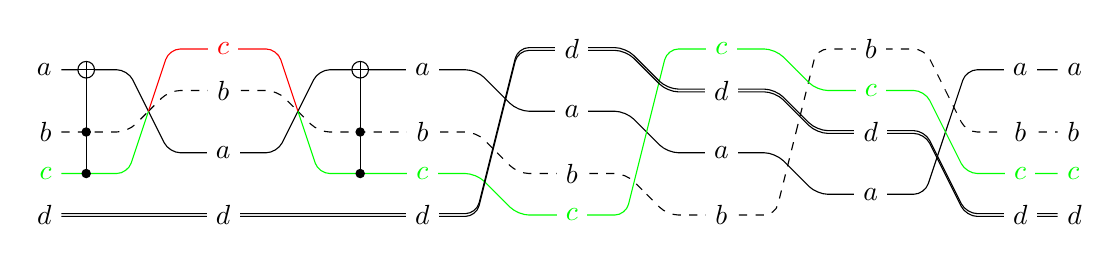
\begin{tikzpicture}[scale=1.000000,x=1pt,y=1pt]
\filldraw[color=white] (0.000000, -7.500000) rectangle (360.000000, 67.500000);
% Drawing wires
% Line 1: a W a a breadth=30
\draw[color=black,rounded corners=4.000000pt] (0.000000,52.500000) -- (24.000000,52.500000) -- (31.500000,37.500000);
\draw[color=black,rounded corners=4.000000pt] (31.500000,37.500000) -- (39.000000,22.500000) -- (78.000000,22.500000) -- (85.500000,37.500000);
\draw[color=black,rounded corners=4.000000pt] (85.500000,37.500000) -- (93.000000,52.500000) -- (150.000000,52.500000) -- (157.500000,45.000000);
\draw[color=black,rounded corners=4.000000pt] (157.500000,45.000000) -- (165.000000,37.500000) -- (204.000000,37.500000) -- (211.500000,30.000000);
\draw[color=black,rounded corners=4.000000pt] (211.500000,30.000000) -- (219.000000,22.500000) -- (258.000000,22.500000) -- (265.500000,15.000000);
\draw[color=black,rounded corners=4.000000pt] (265.500000,15.000000) -- (273.000000,7.500000) -- (312.000000,7.500000) -- (319.500000,30.000000);
\draw[color=black,rounded corners=4.000000pt] (319.500000,30.000000) -- (327.000000,52.500000) -- (360.000000,52.500000);
\draw[color=black] (0.000000,52.500000) node[left] {$a$};
% Line 2: b W b b style=dashed
\draw[color=black,dashed,rounded corners=4.000000pt] (0.000000,30.000000) -- (24.000000,30.000000) -- (31.500000,37.500000);
\draw[color=black,dashed,rounded corners=4.000000pt] (31.500000,37.500000) -- (39.000000,45.000000) -- (78.000000,45.000000) -- (85.500000,37.500000);
\draw[color=black,dashed,rounded corners=4.000000pt] (85.500000,37.500000) -- (93.000000,30.000000) -- (150.000000,30.000000) -- (157.500000,22.500000);
\draw[color=black,dashed,rounded corners=4.000000pt] (157.500000,22.500000) -- (165.000000,15.000000) -- (204.000000,15.000000) -- (211.500000,7.500000);
\draw[color=black,dashed,rounded corners=4.000000pt] (211.500000,7.500000) -- (219.000000,0.000000) -- (258.000000,0.000000) -- (265.500000,30.000000);
\draw[color=black,dashed,rounded corners=4.000000pt] (265.500000,30.000000) -- (273.000000,60.000000) -- (312.000000,60.000000) -- (319.500000,45.000000);
\draw[color=black,dashed,rounded corners=4.000000pt] (319.500000,45.000000) -- (327.000000,30.000000) -- (360.000000,30.000000);
\draw[color=black] (0.000000,30.000000) node[left] {$b$};
% Line 3: c W c c color=green
\draw[color=green,rounded corners=4.000000pt] (0.000000,15.000000) -- (24.000000,15.000000) -- (31.500000,37.500000);
\draw[color=red,rounded corners=4.000000pt] (31.500000,37.500000) -- (39.000000,60.000000) -- (78.000000,60.000000) -- (85.500000,37.500000);
\draw[color=green,rounded corners=4.000000pt] (85.500000,37.500000) -- (93.000000,15.000000) -- (150.000000,15.000000) -- (157.500000,7.500000);
\draw[color=green,rounded corners=4.000000pt] (157.500000,7.500000) -- (165.000000,0.000000) -- (204.000000,0.000000) -- (211.500000,30.000000);
\draw[color=green,rounded corners=4.000000pt] (211.500000,30.000000) -- (219.000000,60.000000) -- (258.000000,60.000000) -- (265.500000,52.500000);
\draw[color=green,rounded corners=4.000000pt] (265.500000,52.500000) -- (273.000000,45.000000) -- (312.000000,45.000000) -- (319.500000,30.000000);
\draw[color=green,rounded corners=4.000000pt] (319.500000,30.000000) -- (327.000000,15.000000) -- (360.000000,15.000000);
\draw[color=green] (0.000000,15.000000) node[left] {$c$};
% Line 4: d W d d type=c
\draw[color=black,rounded corners=4.000000pt] (0.000000,-0.500000) -- (150.000000,-0.500000) -- (157.500000,29.500000);
\draw[color=black,rounded corners=4.000000pt] (0.000000,0.500000) -- (150.000000,0.500000) -- (157.500000,30.500000);
\draw[color=black,rounded corners=4.000000pt] (157.500000,29.500000) -- (165.000000,59.500000) -- (204.000000,59.500000) -- (211.500000,52.000000);
\draw[color=black,rounded corners=4.000000pt] (157.500000,30.500000) -- (165.000000,60.500000) -- (204.000000,60.500000) -- (211.500000,53.000000);
\draw[color=black,rounded corners=4.000000pt] (211.500000,52.000000) -- (219.000000,44.500000) -- (258.000000,44.500000) -- (265.500000,37.000000);
\draw[color=black,rounded corners=4.000000pt] (211.500000,53.000000) -- (219.000000,45.500000) -- (258.000000,45.500000) -- (265.500000,38.000000);
\draw[color=black,rounded corners=4.000000pt] (265.500000,37.000000) -- (273.000000,29.500000) -- (312.000000,29.500000) -- (319.500000,14.500000);
\draw[color=black,rounded corners=4.000000pt] (265.500000,38.000000) -- (273.000000,30.500000) -- (312.000000,30.500000) -- (319.500000,15.500000);
\draw[color=black,rounded corners=4.000000pt] (319.500000,14.500000) -- (327.000000,-0.500000) -- (360.000000,-0.500000);
\draw[color=black,rounded corners=4.000000pt] (319.500000,15.500000) -- (327.000000,0.500000) -- (360.000000,0.500000);
\draw[color=black] (0.000000,0.000000) node[left] {$d$};
% Done with wires; drawing gates
% Line 7: +a b c
\draw (9.000000,52.500000) -- (9.000000,15.000000);
\begin{scope}
\draw[fill=white] (9.000000, 52.500000) circle(3.000000pt);
\clip (9.000000, 52.500000) circle(3.000000pt);
\draw (6.000000, 52.500000) -- (12.000000, 52.500000);
\draw (9.000000, 49.500000) -- (9.000000, 55.500000);
\end{scope}
\filldraw (9.000000, 30.000000) circle(1.500000pt);
\filldraw (9.000000, 15.000000) circle(1.500000pt);
\draw (108.000000,52.500000) -- (108.000000,15.000000);
\begin{scope}
\draw[fill=white] (108.000000, 52.500000) circle(3.000000pt);
\clip (108.000000, 52.500000) circle(3.000000pt);
\draw (105.000000, 52.500000) -- (111.000000, 52.500000);
\draw (108.000000, 49.500000) -- (108.000000, 55.500000);
\end{scope}
\filldraw (108.000000, 30.000000) circle(1.500000pt);
\filldraw (108.000000, 15.000000) circle(1.500000pt);
% Line 8: c a PERMUTE c:color=red
% Line 9: LABEL a b c d
\draw[color=black] (58.500000, 22.500000) node [fill=white] {$a$};
\draw[color=black] (58.500000, 45.000000) node [fill=white] {$b$};
\draw[color=red] (58.500000, 60.000000) node [fill=white] {$c$};
\draw[color=black] (58.500000, 0.000000) node [fill=white] {$d$};
% Line 11: LABEL a b c d
\draw[color=black] (130.500000, 52.500000) node [fill=white] {$a$};
\draw[color=black] (130.500000, 30.000000) node [fill=white] {$b$};
\draw[color=green] (130.500000, 15.000000) node [fill=white] {$c$};
\draw[color=black] (130.500000, 0.000000) node [fill=white] {$d$};
% Line 13: d a b c PERMUTE
% Line 14: LABEL a b c d
\draw[color=black] (184.500000, 37.500000) node [fill=white] {$a$};
\draw[color=black] (184.500000, 15.000000) node [fill=white] {$b$};
\draw[color=green] (184.500000, 0.000000) node [fill=white] {$c$};
\draw[color=black] (184.500000, 60.000000) node [fill=white] {$d$};
\draw[color=black] (238.500000, 22.500000) node [fill=white] {$a$};
\draw[color=black] (238.500000, 0.000000) node [fill=white] {$b$};
\draw[color=green] (238.500000, 60.000000) node [fill=white] {$c$};
\draw[color=black] (238.500000, 45.000000) node [fill=white] {$d$};
\draw[color=black] (292.500000, 7.500000) node [fill=white] {$a$};
\draw[color=black] (292.500000, 60.000000) node [fill=white] {$b$};
\draw[color=green] (292.500000, 45.000000) node [fill=white] {$c$};
\draw[color=black] (292.500000, 30.000000) node [fill=white] {$d$};
\draw[color=black] (346.500000, 52.500000) node [fill=white] {$a$};
\draw[color=black] (346.500000, 30.000000) node [fill=white] {$b$};
\draw[color=green] (346.500000, 15.000000) node [fill=white] {$c$};
\draw[color=black] (346.500000, 0.000000) node [fill=white] {$d$};
% Done with gates; drawing ending labels
\draw[color=black] (360.000000,52.500000) node[right] {$a$};
\draw[color=black] (360.000000,30.000000) node[right] {$b$};
\draw[color=green] (360.000000,15.000000) node[right] {$c$};
\draw[color=black] (360.000000,0.000000) node[right] {$d$};
% Done with ending labels; drawing cut lines and comments
% Done with comments
\end{tikzpicture}

\end{figure}

\SaveVerb{name}|phantom_test|
\begin{figure}[ht]
\caption{\protect\UseVerb{name}}
%! \usetikzlibrary{decorations.pathreplacing,decorations.pathmorphing}
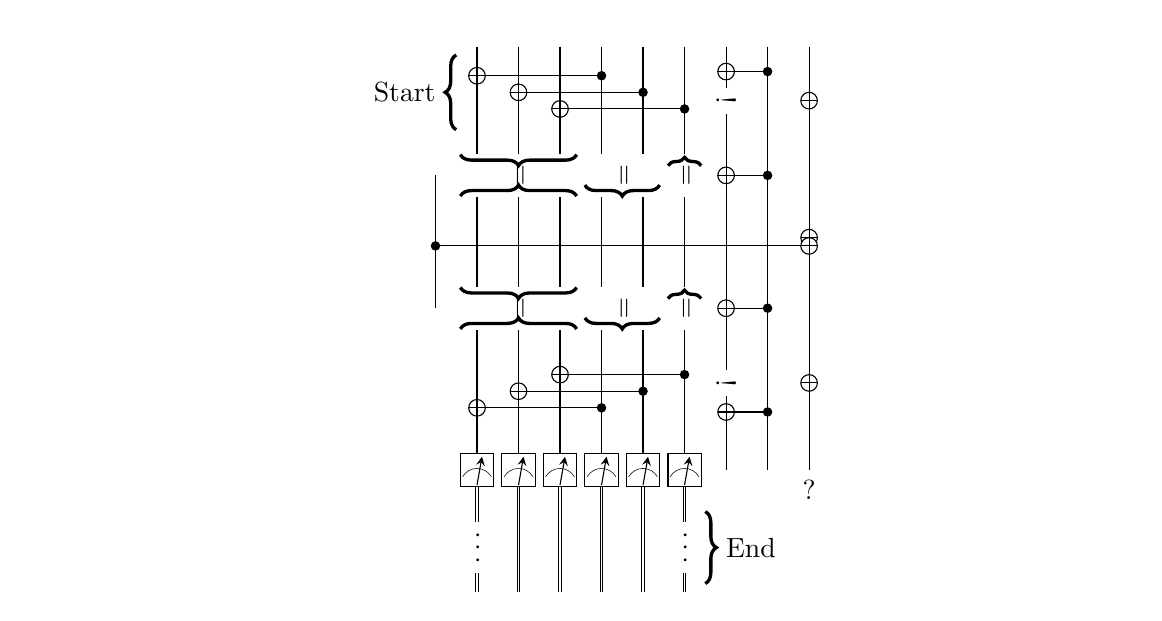
\begin{tikzpicture}[scale=1.000000,x=1pt,y=1pt]
\filldraw[color=white] (7.500000, 0.000000) rectangle (-142.500000, -197.000000);
% Drawing wires
% Line 1: d W
\draw[color=black] (-135.000000,-46.500000) -- (-135.000000,-94.500000);
% Line 2: a0 W
\draw[color=black] (-120.000000,0.000000) -- (-120.000000,-153.000000);
\draw[color=black] (-119.500000,-153.000000) -- (-119.500000,-197.000000);
\draw[color=black] (-120.500000,-153.000000) -- (-120.500000,-197.000000);
% Line 3: a1 W
\draw[color=black] (-105.000000,0.000000) -- (-105.000000,-153.000000);
\draw[color=black] (-104.500000,-153.000000) -- (-104.500000,-197.000000);
\draw[color=black] (-105.500000,-153.000000) -- (-105.500000,-197.000000);
% Line 4: a2 W
\draw[color=black] (-90.000000,0.000000) -- (-90.000000,-153.000000);
\draw[color=black] (-89.500000,-153.000000) -- (-89.500000,-197.000000);
\draw[color=black] (-90.500000,-153.000000) -- (-90.500000,-197.000000);
% Line 5: a3 W
\draw[color=black] (-75.000000,0.000000) -- (-75.000000,-153.000000);
\draw[color=black] (-74.500000,-153.000000) -- (-74.500000,-197.000000);
\draw[color=black] (-75.500000,-153.000000) -- (-75.500000,-197.000000);
% Line 6: a4 W
\draw[color=black] (-60.000000,0.000000) -- (-60.000000,-153.000000);
\draw[color=black] (-59.500000,-153.000000) -- (-59.500000,-197.000000);
\draw[color=black] (-60.500000,-153.000000) -- (-60.500000,-197.000000);
% Line 7: a5 W
\draw[color=black] (-45.000000,0.000000) -- (-45.000000,-153.000000);
\draw[color=black] (-44.500000,-153.000000) -- (-44.500000,-197.000000);
\draw[color=black] (-45.500000,-153.000000) -- (-45.500000,-197.000000);
% Line 8: b0 W
\draw[color=black] (-30.000000,0.000000) -- (-30.000000,-153.000000);
% Line 9: b1 W
\draw[color=black] (-15.000000,0.000000) -- (-15.000000,-153.000000);
% Line 10: c W {} ?
\draw[color=black] (-0.000000,0.000000) -- (-0.000000,-153.000000);
\draw[color=black] (-0.000000,0.000000) node[above] {${}$};
% Done with wires; drawing gates
% Line 13: +a0 a3
\draw (-120.000000,-10.500000) -- (-75.000000,-10.500000);
\begin{scope}
\draw[fill=white] (-120.000000, -10.500000) circle(3.000000pt);
\clip (-120.000000, -10.500000) circle(3.000000pt);
\draw (-123.000000, -10.500000) -- (-117.000000, -10.500000);
\draw (-120.000000, -13.500000) -- (-120.000000, -7.500000);
\end{scope}
\filldraw (-75.000000, -10.500000) circle(1.500000pt);
\draw (-120.000000,-130.500000) -- (-75.000000,-130.500000);
\begin{scope}
\draw[fill=white] (-120.000000, -130.500000) circle(3.000000pt);
\clip (-120.000000, -130.500000) circle(3.000000pt);
\draw (-123.000000, -130.500000) -- (-117.000000, -130.500000);
\draw (-120.000000, -133.500000) -- (-120.000000, -127.500000);
\end{scope}
\filldraw (-75.000000, -130.500000) circle(1.500000pt);
% Line 14: c d PHANTOM
% Line 15: +a1 a4
\draw (-105.000000,-16.500000) -- (-60.000000,-16.500000);
\begin{scope}
\draw[fill=white] (-105.000000, -16.500000) circle(3.000000pt);
\clip (-105.000000, -16.500000) circle(3.000000pt);
\draw (-108.000000, -16.500000) -- (-102.000000, -16.500000);
\draw (-105.000000, -19.500000) -- (-105.000000, -13.500000);
\end{scope}
\filldraw (-60.000000, -16.500000) circle(1.500000pt);
\draw (-105.000000,-124.500000) -- (-60.000000,-124.500000);
\begin{scope}
\draw[fill=white] (-105.000000, -124.500000) circle(3.000000pt);
\clip (-105.000000, -124.500000) circle(3.000000pt);
\draw (-108.000000, -124.500000) -- (-102.000000, -124.500000);
\draw (-105.000000, -127.500000) -- (-105.000000, -121.500000);
\end{scope}
\filldraw (-60.000000, -124.500000) circle(1.500000pt);
% Line 16: +a2 a5
\draw (-90.000000,-22.500000) -- (-45.000000,-22.500000);
\begin{scope}
\draw[fill=white] (-90.000000, -22.500000) circle(3.000000pt);
\clip (-90.000000, -22.500000) circle(3.000000pt);
\draw (-93.000000, -22.500000) -- (-87.000000, -22.500000);
\draw (-90.000000, -25.500000) -- (-90.000000, -19.500000);
\end{scope}
\filldraw (-45.000000, -22.500000) circle(1.500000pt);
\draw (-90.000000,-118.500000) -- (-45.000000,-118.500000);
\begin{scope}
\draw[fill=white] (-90.000000, -118.500000) circle(3.000000pt);
\clip (-90.000000, -118.500000) circle(3.000000pt);
\draw (-93.000000, -118.500000) -- (-87.000000, -118.500000);
\draw (-90.000000, -121.500000) -- (-90.000000, -115.500000);
\end{scope}
\filldraw (-45.000000, -118.500000) circle(1.500000pt);
% Line 18: +b0 b1
\draw (-30.000000,-9.000000) -- (-15.000000,-9.000000);
\begin{scope}
\draw[fill=white] (-30.000000, -9.000000) circle(3.000000pt);
\clip (-30.000000, -9.000000) circle(3.000000pt);
\draw (-33.000000, -9.000000) -- (-27.000000, -9.000000);
\draw (-30.000000, -12.000000) -- (-30.000000, -6.000000);
\end{scope}
\filldraw (-15.000000, -9.000000) circle(1.500000pt);
\draw (-30.000000,-132.000000) -- (-15.000000,-132.000000);
\begin{scope}
\draw[fill=white] (-30.000000, -132.000000) circle(3.000000pt);
\clip (-30.000000, -132.000000) circle(3.000000pt);
\draw (-33.000000, -132.000000) -- (-27.000000, -132.000000);
\draw (-30.000000, -135.000000) -- (-30.000000, -129.000000);
\end{scope}
\filldraw (-15.000000, -132.000000) circle(1.500000pt);
% Line 19: b0 LABEL ! breadth=6
\draw[color=black] (-30.000000, -19.500000) node [fill=white, rotate around={-90:(0,0)}] {$!$};
\draw[color=black] (-30.000000, -121.500000) node [fill=white, rotate around={-90:(0,0)}] {$!$};
% Line 21: +c
\begin{scope}
\draw[fill=white] (-0.000000, -19.500000) circle(3.000000pt);
\clip (-0.000000, -19.500000) circle(3.000000pt);
\draw (-3.000000, -19.500000) -- (3.000000, -19.500000);
\draw (-0.000000, -22.500000) -- (-0.000000, -16.500000);
\end{scope}
\begin{scope}
\draw[fill=white] (-0.000000, -121.500000) circle(3.000000pt);
\clip (-0.000000, -121.500000) circle(3.000000pt);
\draw (-3.000000, -121.500000) -- (3.000000, -121.500000);
\draw (-0.000000, -124.500000) -- (-0.000000, -118.500000);
\end{scope}
% Line 23: a0 a1 a2 >=<
\draw[fill=white,color=white] (-126.000000, -54.000000) rectangle (-84.000000, -39.000000);
\draw (-105.000000, -46.500000) node {\rotatebox{-90}{$=$}};
\draw[decorate,decoration={brace,amplitude = 4.000000pt},very thick] (-84.000000,-39.000000) -- (-126.000000,-39.000000);
\draw[decorate,decoration={brace,mirror,amplitude = 4.000000pt},very thick] (-84.000000,-54.000000) -- (-126.000000,-54.000000);
\draw[fill=white,color=white] (-126.000000, -102.000000) rectangle (-84.000000, -87.000000);
\draw (-105.000000, -94.500000) node {\rotatebox{-90}{$=$}};
\draw[decorate,decoration={brace,amplitude = 4.000000pt},very thick] (-84.000000,-87.000000) -- (-126.000000,-87.000000);
\draw[decorate,decoration={brace,mirror,amplitude = 4.000000pt},very thick] (-84.000000,-102.000000) -- (-126.000000,-102.000000);
% Line 24: a3 a4 =>
\draw[fill=white,color=white] (-81.000000, -54.000000) rectangle (-54.000000, -39.000000);
\draw (-67.500000, -46.500000) node {\rotatebox{-90}{$=$}};
\draw[decorate,decoration={brace,amplitude = 4.000000pt},very thick] (-54.000000,-50.000000) -- (-81.000000,-50.000000);
\draw[fill=white,color=white] (-81.000000, -102.000000) rectangle (-54.000000, -87.000000);
\draw (-67.500000, -94.500000) node {\rotatebox{-90}{$=$}};
\draw[decorate,decoration={brace,amplitude = 4.000000pt},very thick] (-54.000000,-98.000000) -- (-81.000000,-98.000000);
% Line 25: a5 <=
\draw[fill=white,color=white] (-51.000000, -54.000000) rectangle (-39.000000, -39.000000);
\draw (-45.000000, -46.500000) node {\rotatebox{-90}{$=$}};
\draw[decorate,decoration={brace,mirror,amplitude = 3.000000pt},very thick] (-39.000000,-43.000000) -- (-51.000000,-43.000000);
\draw[fill=white,color=white] (-51.000000, -102.000000) rectangle (-39.000000, -87.000000);
\draw (-45.000000, -94.500000) node {\rotatebox{-90}{$=$}};
\draw[decorate,decoration={brace,mirror,amplitude = 3.000000pt},very thick] (-39.000000,-91.000000) -- (-51.000000,-91.000000);
% Line 26: +b0 b1 length=12
\draw (-30.000000,-46.500000) -- (-15.000000,-46.500000);
\begin{scope}
\draw[fill=white] (-30.000000, -46.500000) circle(3.000000pt);
\clip (-30.000000, -46.500000) circle(3.000000pt);
\draw (-33.000000, -46.500000) -- (-27.000000, -46.500000);
\draw (-30.000000, -49.500000) -- (-30.000000, -43.500000);
\end{scope}
\filldraw (-15.000000, -46.500000) circle(1.500000pt);
\draw (-30.000000,-94.500000) -- (-15.000000,-94.500000);
\begin{scope}
\draw[fill=white] (-30.000000, -94.500000) circle(3.000000pt);
\clip (-30.000000, -94.500000) circle(3.000000pt);
\draw (-33.000000, -94.500000) -- (-27.000000, -94.500000);
\draw (-30.000000, -97.500000) -- (-30.000000, -91.500000);
\end{scope}
\filldraw (-15.000000, -94.500000) circle(1.500000pt);
% Line 27: d START
% Line 29: +c
\begin{scope}
\draw[fill=white] (-0.000000, -69.000000) circle(3.000000pt);
\clip (-0.000000, -69.000000) circle(3.000000pt);
\draw (-3.000000, -69.000000) -- (3.000000, -69.000000);
\draw (-0.000000, -72.000000) -- (-0.000000, -66.000000);
\end{scope}
% Line 30: c LABEL length=-3
% Line 31: +c d
\draw (-135.000000,-72.000000) -- (-0.000000,-72.000000);
\begin{scope}
\draw[fill=white] (-0.000000, -72.000000) circle(3.000000pt);
\clip (-0.000000, -72.000000) circle(3.000000pt);
\draw (-3.000000, -72.000000) -- (3.000000, -72.000000);
\draw (-0.000000, -75.000000) -- (-0.000000, -69.000000);
\end{scope}
\filldraw (-135.000000, -72.000000) circle(1.500000pt);
% Line 34: TOUCH
% Line 35: b0 b1 c END length=0
\draw[color=black] (-0.000000,-153.000000) node[fill=white,below,minimum width=15.000000pt,minimum height=0.000000pt,inner sep=0pt] {\phantom{$?$}};
\draw[color=black] (-0.000000,-153.000000) node[below] {$?$};
% Line 36: a0 a1 a2 a3 a4 a5 M
\draw[fill=white] (-126.000000, -159.000000) rectangle (-114.000000, -147.000000);
\draw[very thin] (-120.000000, -152.400000) arc (90:150:6.000000pt);
\draw[very thin] (-120.000000, -152.400000) arc (90:30:6.000000pt);
\draw[->,>=stealth] (-120.000000, -158.400000) -- +(80:10.392305pt);
\draw[fill=white] (-111.000000, -159.000000) rectangle (-99.000000, -147.000000);
\draw[very thin] (-105.000000, -152.400000) arc (90:150:6.000000pt);
\draw[very thin] (-105.000000, -152.400000) arc (90:30:6.000000pt);
\draw[->,>=stealth] (-105.000000, -158.400000) -- +(80:10.392305pt);
\draw[fill=white] (-96.000000, -159.000000) rectangle (-84.000000, -147.000000);
\draw[very thin] (-90.000000, -152.400000) arc (90:150:6.000000pt);
\draw[very thin] (-90.000000, -152.400000) arc (90:30:6.000000pt);
\draw[->,>=stealth] (-90.000000, -158.400000) -- +(80:10.392305pt);
\draw[fill=white] (-81.000000, -159.000000) rectangle (-69.000000, -147.000000);
\draw[very thin] (-75.000000, -152.400000) arc (90:150:6.000000pt);
\draw[very thin] (-75.000000, -152.400000) arc (90:30:6.000000pt);
\draw[->,>=stealth] (-75.000000, -158.400000) -- +(80:10.392305pt);
\draw[fill=white] (-66.000000, -159.000000) rectangle (-54.000000, -147.000000);
\draw[very thin] (-60.000000, -152.400000) arc (90:150:6.000000pt);
\draw[very thin] (-60.000000, -152.400000) arc (90:30:6.000000pt);
\draw[->,>=stealth] (-60.000000, -158.400000) -- +(80:10.392305pt);
\draw[fill=white] (-51.000000, -159.000000) rectangle (-39.000000, -147.000000);
\draw[very thin] (-45.000000, -152.400000) arc (90:150:6.000000pt);
\draw[very thin] (-45.000000, -152.400000) arc (90:30:6.000000pt);
\draw[->,>=stealth] (-45.000000, -158.400000) -- +(80:10.392305pt);
% Line 37: a0 a5 LABEL ... length=20
\draw[color=black] (-120.000000, -181.000000) node [fill=white, rotate around={-90:(0,0)}] {$\cdots$};
\draw[color=black] (-45.000000, -181.000000) node [fill=white, rotate around={-90:(0,0)}] {$\cdots$};
% Done with gates; drawing ending labels
% Done with ending labels; drawing cut lines and comments
% Line 38: a0 a5 @ 1 %% End
\draw[decorate,decoration={brace,amplitude = 4.000000pt},very thick] (-37.500000,-168.000000) -- (-37.500000,-194.000000);
\draw (-33.500000, -181.000000) node[text width=144pt,right] {End};
% Line 39: a0 a5 @ 0 0 % Start
\draw[decorate,decoration={brace,mirror,amplitude = 4.000000pt},very thick] (-127.500000,-3.000000) -- (-127.500000,-30.000000);
\draw (-131.500000, -16.500000) node[text width=144pt,left,text ragged left] {Start};
% Done with comments
\end{tikzpicture}

\end{figure}
\clearpage

\SaveVerb{name}|reverse-8|
\begin{figure}[ht]
\caption{\protect\UseVerb{name}}
\providecommand{\bit}[1]{{\left\langle{#1}\right\rangle}}
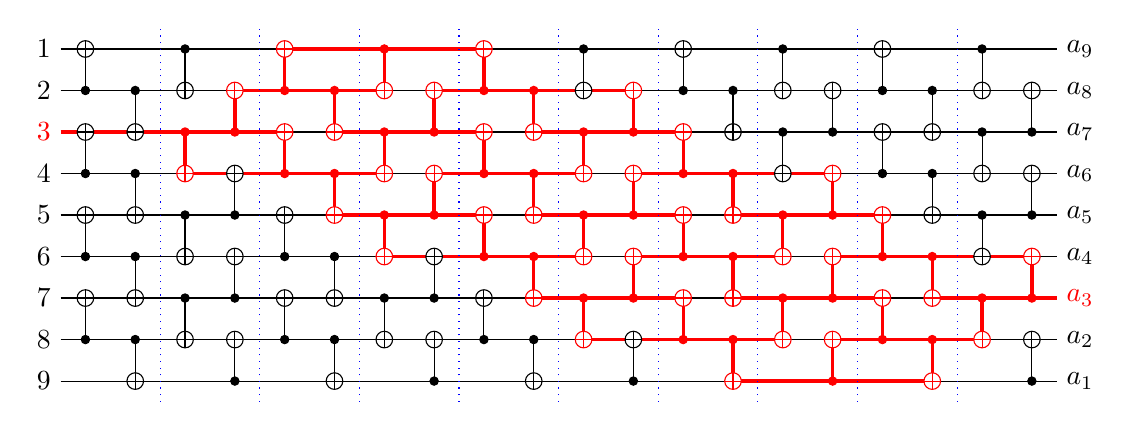
\begin{tikzpicture}[scale=1.000000,x=1pt,y=1pt]
\filldraw[color=white] (0.000000, -7.500000) rectangle (360.000000, 127.500000);
% Drawing wires
% Line 5: 1 W \bit{1} a_9
\draw[color=black] (0.000000,120.000000) -- (81.000000,120.000000);
\draw[color=red,very thick] (81.000000,120.000000) -- (153.000000,120.000000);
\draw[color=black,thin] (153.000000,120.000000) -- (360.000000,120.000000);
\draw[color=black] (0.000000,120.000000) node[left] {$\bit{1}$};
% Line 6: 2 W \bit{2} a_8
\draw[color=black] (0.000000,105.000000) -- (63.000000,105.000000);
\draw[color=red,very thick] (63.000000,105.000000) -- (117.000000,105.000000);
\draw[color=black,thin] (117.000000,105.000000) -- (135.000000,105.000000);
\draw[color=red,very thick] (135.000000,105.000000) -- (207.000000,105.000000);
\draw[color=black,thin] (207.000000,105.000000) -- (360.000000,105.000000);
\draw[color=black] (0.000000,105.000000) node[left] {$\bit{2}$};
% Line 7: 3 W \bit{3} a_7 on
\draw[color=red,very thick] (0.000000,90.000000) -- (81.000000,90.000000);
\draw[color=black,thin] (81.000000,90.000000) -- (99.000000,90.000000);
\draw[color=red,very thick] (99.000000,90.000000) -- (153.000000,90.000000);
\draw[color=black,thin] (153.000000,90.000000) -- (171.000000,90.000000);
\draw[color=red,very thick] (171.000000,90.000000) -- (225.000000,90.000000);
\draw[color=black,thin] (225.000000,90.000000) -- (360.000000,90.000000);
\draw[color=red] (0.000000,90.000000) node[left] {$\bit{3}$};
% Line 8: 4 W \bit{4} a_6
\draw[color=black] (0.000000,75.000000) -- (45.000000,75.000000);
\draw[color=red,very thick] (45.000000,75.000000) -- (117.000000,75.000000);
\draw[color=black,thin] (117.000000,75.000000) -- (135.000000,75.000000);
\draw[color=red,very thick] (135.000000,75.000000) -- (189.000000,75.000000);
\draw[color=black,thin] (189.000000,75.000000) -- (207.000000,75.000000);
\draw[color=red,very thick] (207.000000,75.000000) -- (279.000000,75.000000);
\draw[color=black,thin] (279.000000,75.000000) -- (360.000000,75.000000);
\draw[color=black] (0.000000,75.000000) node[left] {$\bit{4}$};
% Line 9: 5 W \bit{5} a_5
\draw[color=black] (0.000000,60.000000) -- (99.000000,60.000000);
\draw[color=red,very thick] (99.000000,60.000000) -- (153.000000,60.000000);
\draw[color=black,thin] (153.000000,60.000000) -- (171.000000,60.000000);
\draw[color=red,very thick] (171.000000,60.000000) -- (225.000000,60.000000);
\draw[color=black,thin] (225.000000,60.000000) -- (243.000000,60.000000);
\draw[color=red,very thick] (243.000000,60.000000) -- (297.000000,60.000000);
\draw[color=black,thin] (297.000000,60.000000) -- (360.000000,60.000000);
\draw[color=black] (0.000000,60.000000) node[left] {$\bit{5}$};
% Line 10: 6 W \bit{6} a_4
\draw[color=black] (0.000000,45.000000) -- (117.000000,45.000000);
\draw[color=red,very thick] (117.000000,45.000000) -- (189.000000,45.000000);
\draw[color=black,thin] (189.000000,45.000000) -- (207.000000,45.000000);
\draw[color=red,very thick] (207.000000,45.000000) -- (261.000000,45.000000);
\draw[color=black,thin] (261.000000,45.000000) -- (279.000000,45.000000);
\draw[color=red,very thick] (279.000000,45.000000) -- (351.000000,45.000000);
\draw[color=black,thin] (351.000000,45.000000) -- (360.000000,45.000000);
\draw[color=black] (0.000000,45.000000) node[left] {$\bit{6}$};
% Line 11: 7 W \bit{7} a_3
\draw[color=black] (0.000000,30.000000) -- (171.000000,30.000000);
\draw[color=red,very thick] (171.000000,30.000000) -- (225.000000,30.000000);
\draw[color=black,thin] (225.000000,30.000000) -- (243.000000,30.000000);
\draw[color=red,very thick] (243.000000,30.000000) -- (297.000000,30.000000);
\draw[color=black,thin] (297.000000,30.000000) -- (315.000000,30.000000);
\draw[color=red,very thick] (315.000000,30.000000) -- (360.000000,30.000000);
\draw[color=black] (0.000000,30.000000) node[left] {$\bit{7}$};
% Line 12: 8 W \bit{8} a_2
\draw[color=black] (0.000000,15.000000) -- (189.000000,15.000000);
\draw[color=red,very thick] (189.000000,15.000000) -- (261.000000,15.000000);
\draw[color=black,thin] (261.000000,15.000000) -- (279.000000,15.000000);
\draw[color=red,very thick] (279.000000,15.000000) -- (333.000000,15.000000);
\draw[color=black,thin] (333.000000,15.000000) -- (360.000000,15.000000);
\draw[color=black] (0.000000,15.000000) node[left] {$\bit{8}$};
% Line 13: 9 W \bit{9} a_1
\draw[color=black] (0.000000,0.000000) -- (243.000000,0.000000);
\draw[color=red,very thick] (243.000000,0.000000) -- (315.000000,0.000000);
\draw[color=black,thin] (315.000000,0.000000) -- (360.000000,0.000000);
\draw[color=black] (0.000000,0.000000) node[left] {$\bit{9}$};
% Done with wires; drawing gates
% Line 17: +1 2
\draw (9.000000,120.000000) -- (9.000000,105.000000);
\begin{scope}
\draw[fill=white] (9.000000, 120.000000) circle(3.000000pt);
\clip (9.000000, 120.000000) circle(3.000000pt);
\draw (6.000000, 120.000000) -- (12.000000, 120.000000);
\draw (9.000000, 117.000000) -- (9.000000, 123.000000);
\end{scope}
\filldraw (9.000000, 105.000000) circle(1.500000pt);
% Line 18: +3 4
\draw (9.000000,90.000000) -- (9.000000,75.000000);
\begin{scope}
\draw[fill=white] (9.000000, 90.000000) circle(3.000000pt);
\clip (9.000000, 90.000000) circle(3.000000pt);
\draw (6.000000, 90.000000) -- (12.000000, 90.000000);
\draw (9.000000, 87.000000) -- (9.000000, 93.000000);
\end{scope}
\filldraw (9.000000, 75.000000) circle(1.500000pt);
% Line 19: +5 6
\draw (9.000000,60.000000) -- (9.000000,45.000000);
\begin{scope}
\draw[fill=white] (9.000000, 60.000000) circle(3.000000pt);
\clip (9.000000, 60.000000) circle(3.000000pt);
\draw (6.000000, 60.000000) -- (12.000000, 60.000000);
\draw (9.000000, 57.000000) -- (9.000000, 63.000000);
\end{scope}
\filldraw (9.000000, 45.000000) circle(1.500000pt);
% Line 20: +7 8
\draw (9.000000,30.000000) -- (9.000000,15.000000);
\begin{scope}
\draw[fill=white] (9.000000, 30.000000) circle(3.000000pt);
\clip (9.000000, 30.000000) circle(3.000000pt);
\draw (6.000000, 30.000000) -- (12.000000, 30.000000);
\draw (9.000000, 27.000000) -- (9.000000, 33.000000);
\end{scope}
\filldraw (9.000000, 15.000000) circle(1.500000pt);
% Line 21: +3 2
\draw (27.000000,105.000000) -- (27.000000,90.000000);
\begin{scope}
\draw[fill=white] (27.000000, 90.000000) circle(3.000000pt);
\clip (27.000000, 90.000000) circle(3.000000pt);
\draw (24.000000, 90.000000) -- (30.000000, 90.000000);
\draw (27.000000, 87.000000) -- (27.000000, 93.000000);
\end{scope}
\filldraw (27.000000, 105.000000) circle(1.500000pt);
% Line 22: +5 4
\draw (27.000000,75.000000) -- (27.000000,60.000000);
\begin{scope}
\draw[fill=white] (27.000000, 60.000000) circle(3.000000pt);
\clip (27.000000, 60.000000) circle(3.000000pt);
\draw (24.000000, 60.000000) -- (30.000000, 60.000000);
\draw (27.000000, 57.000000) -- (27.000000, 63.000000);
\end{scope}
\filldraw (27.000000, 75.000000) circle(1.500000pt);
% Line 23: +7 6
\draw (27.000000,45.000000) -- (27.000000,30.000000);
\begin{scope}
\draw[fill=white] (27.000000, 30.000000) circle(3.000000pt);
\clip (27.000000, 30.000000) circle(3.000000pt);
\draw (24.000000, 30.000000) -- (30.000000, 30.000000);
\draw (27.000000, 27.000000) -- (27.000000, 33.000000);
\end{scope}
\filldraw (27.000000, 45.000000) circle(1.500000pt);
% Line 24: +9 8
\draw (27.000000,15.000000) -- (27.000000,0.000000);
\begin{scope}
\draw[fill=white] (27.000000, 0.000000) circle(3.000000pt);
\clip (27.000000, 0.000000) circle(3.000000pt);
\draw (24.000000, 0.000000) -- (30.000000, 0.000000);
\draw (27.000000, -3.000000) -- (27.000000, 3.000000);
\end{scope}
\filldraw (27.000000, 15.000000) circle(1.500000pt);
% Line 27: +2 1
\draw (45.000000,120.000000) -- (45.000000,105.000000);
\begin{scope}
\draw[fill=white] (45.000000, 105.000000) circle(3.000000pt);
\clip (45.000000, 105.000000) circle(3.000000pt);
\draw (42.000000, 105.000000) -- (48.000000, 105.000000);
\draw (45.000000, 102.000000) -- (45.000000, 108.000000);
\end{scope}
\filldraw (45.000000, 120.000000) circle(1.500000pt);
% Line 28: +4:on 3 on
\begin{scope}[color=red]
\draw[very thick] (45.000000,90.000000) -- (45.000000,75.000000);
\begin{scope}
\draw[fill=white] (45.000000, 75.000000) circle(3.000000pt);
\clip (45.000000, 75.000000) circle(3.000000pt);
\draw (42.000000, 75.000000) -- (48.000000, 75.000000);
\draw (45.000000, 72.000000) -- (45.000000, 78.000000);
\end{scope}
\filldraw (45.000000, 90.000000) circle(1.500000pt);
\end{scope}
% Line 29: +6 5
\draw (45.000000,60.000000) -- (45.000000,45.000000);
\begin{scope}
\draw[fill=white] (45.000000, 45.000000) circle(3.000000pt);
\clip (45.000000, 45.000000) circle(3.000000pt);
\draw (42.000000, 45.000000) -- (48.000000, 45.000000);
\draw (45.000000, 42.000000) -- (45.000000, 48.000000);
\end{scope}
\filldraw (45.000000, 60.000000) circle(1.500000pt);
% Line 30: +8 7
\draw (45.000000,30.000000) -- (45.000000,15.000000);
\begin{scope}
\draw[fill=white] (45.000000, 15.000000) circle(3.000000pt);
\clip (45.000000, 15.000000) circle(3.000000pt);
\draw (42.000000, 15.000000) -- (48.000000, 15.000000);
\draw (45.000000, 12.000000) -- (45.000000, 18.000000);
\end{scope}
\filldraw (45.000000, 30.000000) circle(1.500000pt);
% Line 31: +2:on 3 on
\begin{scope}[color=red]
\draw[very thick] (63.000000,105.000000) -- (63.000000,90.000000);
\begin{scope}
\draw[fill=white] (63.000000, 105.000000) circle(3.000000pt);
\clip (63.000000, 105.000000) circle(3.000000pt);
\draw (60.000000, 105.000000) -- (66.000000, 105.000000);
\draw (63.000000, 102.000000) -- (63.000000, 108.000000);
\end{scope}
\filldraw (63.000000, 90.000000) circle(1.500000pt);
\end{scope}
% Line 32: +4 5
\draw (63.000000,75.000000) -- (63.000000,60.000000);
\begin{scope}
\draw[fill=white] (63.000000, 75.000000) circle(3.000000pt);
\clip (63.000000, 75.000000) circle(3.000000pt);
\draw (60.000000, 75.000000) -- (66.000000, 75.000000);
\draw (63.000000, 72.000000) -- (63.000000, 78.000000);
\end{scope}
\filldraw (63.000000, 60.000000) circle(1.500000pt);
% Line 33: +6 7
\draw (63.000000,45.000000) -- (63.000000,30.000000);
\begin{scope}
\draw[fill=white] (63.000000, 45.000000) circle(3.000000pt);
\clip (63.000000, 45.000000) circle(3.000000pt);
\draw (60.000000, 45.000000) -- (66.000000, 45.000000);
\draw (63.000000, 42.000000) -- (63.000000, 48.000000);
\end{scope}
\filldraw (63.000000, 30.000000) circle(1.500000pt);
% Line 34: +8 9
\draw (63.000000,15.000000) -- (63.000000,0.000000);
\begin{scope}
\draw[fill=white] (63.000000, 15.000000) circle(3.000000pt);
\clip (63.000000, 15.000000) circle(3.000000pt);
\draw (60.000000, 15.000000) -- (66.000000, 15.000000);
\draw (63.000000, 12.000000) -- (63.000000, 18.000000);
\end{scope}
\filldraw (63.000000, 0.000000) circle(1.500000pt);
% Line 37: +1:on 2 on
\begin{scope}[color=red]
\draw[very thick] (81.000000,120.000000) -- (81.000000,105.000000);
\begin{scope}
\draw[fill=white] (81.000000, 120.000000) circle(3.000000pt);
\clip (81.000000, 120.000000) circle(3.000000pt);
\draw (78.000000, 120.000000) -- (84.000000, 120.000000);
\draw (81.000000, 117.000000) -- (81.000000, 123.000000);
\end{scope}
\filldraw (81.000000, 105.000000) circle(1.500000pt);
\end{scope}
% Line 38: +3:off 4 on
\begin{scope}[color=red]
\draw[very thick] (81.000000,90.000000) -- (81.000000,75.000000);
\begin{scope}
\draw[fill=white] (81.000000, 90.000000) circle(3.000000pt);
\clip (81.000000, 90.000000) circle(3.000000pt);
\draw (78.000000, 90.000000) -- (84.000000, 90.000000);
\draw (81.000000, 87.000000) -- (81.000000, 93.000000);
\end{scope}
\filldraw (81.000000, 75.000000) circle(1.500000pt);
\end{scope}
% Line 39: +5 6
\draw (81.000000,60.000000) -- (81.000000,45.000000);
\begin{scope}
\draw[fill=white] (81.000000, 60.000000) circle(3.000000pt);
\clip (81.000000, 60.000000) circle(3.000000pt);
\draw (78.000000, 60.000000) -- (84.000000, 60.000000);
\draw (81.000000, 57.000000) -- (81.000000, 63.000000);
\end{scope}
\filldraw (81.000000, 45.000000) circle(1.500000pt);
% Line 40: +7 8
\draw (81.000000,30.000000) -- (81.000000,15.000000);
\begin{scope}
\draw[fill=white] (81.000000, 30.000000) circle(3.000000pt);
\clip (81.000000, 30.000000) circle(3.000000pt);
\draw (78.000000, 30.000000) -- (84.000000, 30.000000);
\draw (81.000000, 27.000000) -- (81.000000, 33.000000);
\end{scope}
\filldraw (81.000000, 15.000000) circle(1.500000pt);
% Line 41: +3:on 2 on
\begin{scope}[color=red]
\draw[very thick] (99.000000,105.000000) -- (99.000000,90.000000);
\begin{scope}
\draw[fill=white] (99.000000, 90.000000) circle(3.000000pt);
\clip (99.000000, 90.000000) circle(3.000000pt);
\draw (96.000000, 90.000000) -- (102.000000, 90.000000);
\draw (99.000000, 87.000000) -- (99.000000, 93.000000);
\end{scope}
\filldraw (99.000000, 105.000000) circle(1.500000pt);
\end{scope}
% Line 42: +5:on 4 on
\begin{scope}[color=red]
\draw[very thick] (99.000000,75.000000) -- (99.000000,60.000000);
\begin{scope}
\draw[fill=white] (99.000000, 60.000000) circle(3.000000pt);
\clip (99.000000, 60.000000) circle(3.000000pt);
\draw (96.000000, 60.000000) -- (102.000000, 60.000000);
\draw (99.000000, 57.000000) -- (99.000000, 63.000000);
\end{scope}
\filldraw (99.000000, 75.000000) circle(1.500000pt);
\end{scope}
% Line 43: +7 6
\draw (99.000000,45.000000) -- (99.000000,30.000000);
\begin{scope}
\draw[fill=white] (99.000000, 30.000000) circle(3.000000pt);
\clip (99.000000, 30.000000) circle(3.000000pt);
\draw (96.000000, 30.000000) -- (102.000000, 30.000000);
\draw (99.000000, 27.000000) -- (99.000000, 33.000000);
\end{scope}
\filldraw (99.000000, 45.000000) circle(1.500000pt);
% Line 44: +9 8
\draw (99.000000,15.000000) -- (99.000000,0.000000);
\begin{scope}
\draw[fill=white] (99.000000, 0.000000) circle(3.000000pt);
\clip (99.000000, 0.000000) circle(3.000000pt);
\draw (96.000000, 0.000000) -- (102.000000, 0.000000);
\draw (99.000000, -3.000000) -- (99.000000, 3.000000);
\end{scope}
\filldraw (99.000000, 15.000000) circle(1.500000pt);
% Line 47: +2:off 1 on
\begin{scope}[color=red]
\draw[very thick] (117.000000,120.000000) -- (117.000000,105.000000);
\begin{scope}
\draw[fill=white] (117.000000, 105.000000) circle(3.000000pt);
\clip (117.000000, 105.000000) circle(3.000000pt);
\draw (114.000000, 105.000000) -- (120.000000, 105.000000);
\draw (117.000000, 102.000000) -- (117.000000, 108.000000);
\end{scope}
\filldraw (117.000000, 120.000000) circle(1.500000pt);
\end{scope}
% Line 48: +4:off 3 on
\begin{scope}[color=red]
\draw[very thick] (117.000000,90.000000) -- (117.000000,75.000000);
\begin{scope}
\draw[fill=white] (117.000000, 75.000000) circle(3.000000pt);
\clip (117.000000, 75.000000) circle(3.000000pt);
\draw (114.000000, 75.000000) -- (120.000000, 75.000000);
\draw (117.000000, 72.000000) -- (117.000000, 78.000000);
\end{scope}
\filldraw (117.000000, 90.000000) circle(1.500000pt);
\end{scope}
% Line 49: +6:on 5 on
\begin{scope}[color=red]
\draw[very thick] (117.000000,60.000000) -- (117.000000,45.000000);
\begin{scope}
\draw[fill=white] (117.000000, 45.000000) circle(3.000000pt);
\clip (117.000000, 45.000000) circle(3.000000pt);
\draw (114.000000, 45.000000) -- (120.000000, 45.000000);
\draw (117.000000, 42.000000) -- (117.000000, 48.000000);
\end{scope}
\filldraw (117.000000, 60.000000) circle(1.500000pt);
\end{scope}
% Line 50: +8 7
\draw (117.000000,30.000000) -- (117.000000,15.000000);
\begin{scope}
\draw[fill=white] (117.000000, 15.000000) circle(3.000000pt);
\clip (117.000000, 15.000000) circle(3.000000pt);
\draw (114.000000, 15.000000) -- (120.000000, 15.000000);
\draw (117.000000, 12.000000) -- (117.000000, 18.000000);
\end{scope}
\filldraw (117.000000, 30.000000) circle(1.500000pt);
% Line 51: +2:on 3 on
\begin{scope}[color=red]
\draw[very thick] (135.000000,105.000000) -- (135.000000,90.000000);
\begin{scope}
\draw[fill=white] (135.000000, 105.000000) circle(3.000000pt);
\clip (135.000000, 105.000000) circle(3.000000pt);
\draw (132.000000, 105.000000) -- (138.000000, 105.000000);
\draw (135.000000, 102.000000) -- (135.000000, 108.000000);
\end{scope}
\filldraw (135.000000, 90.000000) circle(1.500000pt);
\end{scope}
% Line 52: +4:on 5 on
\begin{scope}[color=red]
\draw[very thick] (135.000000,75.000000) -- (135.000000,60.000000);
\begin{scope}
\draw[fill=white] (135.000000, 75.000000) circle(3.000000pt);
\clip (135.000000, 75.000000) circle(3.000000pt);
\draw (132.000000, 75.000000) -- (138.000000, 75.000000);
\draw (135.000000, 72.000000) -- (135.000000, 78.000000);
\end{scope}
\filldraw (135.000000, 60.000000) circle(1.500000pt);
\end{scope}
% Line 53: +6 7
\draw (135.000000,45.000000) -- (135.000000,30.000000);
\begin{scope}
\draw[fill=white] (135.000000, 45.000000) circle(3.000000pt);
\clip (135.000000, 45.000000) circle(3.000000pt);
\draw (132.000000, 45.000000) -- (138.000000, 45.000000);
\draw (135.000000, 42.000000) -- (135.000000, 48.000000);
\end{scope}
\filldraw (135.000000, 30.000000) circle(1.500000pt);
% Line 54: +8 9
\draw (135.000000,15.000000) -- (135.000000,0.000000);
\begin{scope}
\draw[fill=white] (135.000000, 15.000000) circle(3.000000pt);
\clip (135.000000, 15.000000) circle(3.000000pt);
\draw (132.000000, 15.000000) -- (138.000000, 15.000000);
\draw (135.000000, 12.000000) -- (135.000000, 18.000000);
\end{scope}
\filldraw (135.000000, 0.000000) circle(1.500000pt);
% Line 57: +1:off 2 on
\begin{scope}[color=red]
\draw[very thick] (153.000000,120.000000) -- (153.000000,105.000000);
\begin{scope}
\draw[fill=white] (153.000000, 120.000000) circle(3.000000pt);
\clip (153.000000, 120.000000) circle(3.000000pt);
\draw (150.000000, 120.000000) -- (156.000000, 120.000000);
\draw (153.000000, 117.000000) -- (153.000000, 123.000000);
\end{scope}
\filldraw (153.000000, 105.000000) circle(1.500000pt);
\end{scope}
% Line 58: +3:off 4 on
\begin{scope}[color=red]
\draw[very thick] (153.000000,90.000000) -- (153.000000,75.000000);
\begin{scope}
\draw[fill=white] (153.000000, 90.000000) circle(3.000000pt);
\clip (153.000000, 90.000000) circle(3.000000pt);
\draw (150.000000, 90.000000) -- (156.000000, 90.000000);
\draw (153.000000, 87.000000) -- (153.000000, 93.000000);
\end{scope}
\filldraw (153.000000, 75.000000) circle(1.500000pt);
\end{scope}
% Line 59: +5:off 6 on
\begin{scope}[color=red]
\draw[very thick] (153.000000,60.000000) -- (153.000000,45.000000);
\begin{scope}
\draw[fill=white] (153.000000, 60.000000) circle(3.000000pt);
\clip (153.000000, 60.000000) circle(3.000000pt);
\draw (150.000000, 60.000000) -- (156.000000, 60.000000);
\draw (153.000000, 57.000000) -- (153.000000, 63.000000);
\end{scope}
\filldraw (153.000000, 45.000000) circle(1.500000pt);
\end{scope}
% Line 60: +7 8
\draw (153.000000,30.000000) -- (153.000000,15.000000);
\begin{scope}
\draw[fill=white] (153.000000, 30.000000) circle(3.000000pt);
\clip (153.000000, 30.000000) circle(3.000000pt);
\draw (150.000000, 30.000000) -- (156.000000, 30.000000);
\draw (153.000000, 27.000000) -- (153.000000, 33.000000);
\end{scope}
\filldraw (153.000000, 15.000000) circle(1.500000pt);
% Line 61: +3:on 2 on
\begin{scope}[color=red]
\draw[very thick] (171.000000,105.000000) -- (171.000000,90.000000);
\begin{scope}
\draw[fill=white] (171.000000, 90.000000) circle(3.000000pt);
\clip (171.000000, 90.000000) circle(3.000000pt);
\draw (168.000000, 90.000000) -- (174.000000, 90.000000);
\draw (171.000000, 87.000000) -- (171.000000, 93.000000);
\end{scope}
\filldraw (171.000000, 105.000000) circle(1.500000pt);
\end{scope}
% Line 62: +5:on 4 on
\begin{scope}[color=red]
\draw[very thick] (171.000000,75.000000) -- (171.000000,60.000000);
\begin{scope}
\draw[fill=white] (171.000000, 60.000000) circle(3.000000pt);
\clip (171.000000, 60.000000) circle(3.000000pt);
\draw (168.000000, 60.000000) -- (174.000000, 60.000000);
\draw (171.000000, 57.000000) -- (171.000000, 63.000000);
\end{scope}
\filldraw (171.000000, 75.000000) circle(1.500000pt);
\end{scope}
% Line 63: +7:on 6 on
\begin{scope}[color=red]
\draw[very thick] (171.000000,45.000000) -- (171.000000,30.000000);
\begin{scope}
\draw[fill=white] (171.000000, 30.000000) circle(3.000000pt);
\clip (171.000000, 30.000000) circle(3.000000pt);
\draw (168.000000, 30.000000) -- (174.000000, 30.000000);
\draw (171.000000, 27.000000) -- (171.000000, 33.000000);
\end{scope}
\filldraw (171.000000, 45.000000) circle(1.500000pt);
\end{scope}
% Line 64: +9 8
\draw (171.000000,15.000000) -- (171.000000,0.000000);
\begin{scope}
\draw[fill=white] (171.000000, 0.000000) circle(3.000000pt);
\clip (171.000000, 0.000000) circle(3.000000pt);
\draw (168.000000, 0.000000) -- (174.000000, 0.000000);
\draw (171.000000, -3.000000) -- (171.000000, 3.000000);
\end{scope}
\filldraw (171.000000, 15.000000) circle(1.500000pt);
% Line 67: +2 1
\draw (189.000000,120.000000) -- (189.000000,105.000000);
\begin{scope}
\draw[fill=white] (189.000000, 105.000000) circle(3.000000pt);
\clip (189.000000, 105.000000) circle(3.000000pt);
\draw (186.000000, 105.000000) -- (192.000000, 105.000000);
\draw (189.000000, 102.000000) -- (189.000000, 108.000000);
\end{scope}
\filldraw (189.000000, 120.000000) circle(1.500000pt);
% Line 68: +4:off 3 on
\begin{scope}[color=red]
\draw[very thick] (189.000000,90.000000) -- (189.000000,75.000000);
\begin{scope}
\draw[fill=white] (189.000000, 75.000000) circle(3.000000pt);
\clip (189.000000, 75.000000) circle(3.000000pt);
\draw (186.000000, 75.000000) -- (192.000000, 75.000000);
\draw (189.000000, 72.000000) -- (189.000000, 78.000000);
\end{scope}
\filldraw (189.000000, 90.000000) circle(1.500000pt);
\end{scope}
% Line 69: +6:off 5 on
\begin{scope}[color=red]
\draw[very thick] (189.000000,60.000000) -- (189.000000,45.000000);
\begin{scope}
\draw[fill=white] (189.000000, 45.000000) circle(3.000000pt);
\clip (189.000000, 45.000000) circle(3.000000pt);
\draw (186.000000, 45.000000) -- (192.000000, 45.000000);
\draw (189.000000, 42.000000) -- (189.000000, 48.000000);
\end{scope}
\filldraw (189.000000, 60.000000) circle(1.500000pt);
\end{scope}
% Line 70: +8:on 7 on
\begin{scope}[color=red]
\draw[very thick] (189.000000,30.000000) -- (189.000000,15.000000);
\begin{scope}
\draw[fill=white] (189.000000, 15.000000) circle(3.000000pt);
\clip (189.000000, 15.000000) circle(3.000000pt);
\draw (186.000000, 15.000000) -- (192.000000, 15.000000);
\draw (189.000000, 12.000000) -- (189.000000, 18.000000);
\end{scope}
\filldraw (189.000000, 30.000000) circle(1.500000pt);
\end{scope}
% Line 71: +2:off 3 on
\begin{scope}[color=red]
\draw[very thick] (207.000000,105.000000) -- (207.000000,90.000000);
\begin{scope}
\draw[fill=white] (207.000000, 105.000000) circle(3.000000pt);
\clip (207.000000, 105.000000) circle(3.000000pt);
\draw (204.000000, 105.000000) -- (210.000000, 105.000000);
\draw (207.000000, 102.000000) -- (207.000000, 108.000000);
\end{scope}
\filldraw (207.000000, 90.000000) circle(1.500000pt);
\end{scope}
% Line 72: +4:on 5 on
\begin{scope}[color=red]
\draw[very thick] (207.000000,75.000000) -- (207.000000,60.000000);
\begin{scope}
\draw[fill=white] (207.000000, 75.000000) circle(3.000000pt);
\clip (207.000000, 75.000000) circle(3.000000pt);
\draw (204.000000, 75.000000) -- (210.000000, 75.000000);
\draw (207.000000, 72.000000) -- (207.000000, 78.000000);
\end{scope}
\filldraw (207.000000, 60.000000) circle(1.500000pt);
\end{scope}
% Line 73: +6:on 7 on
\begin{scope}[color=red]
\draw[very thick] (207.000000,45.000000) -- (207.000000,30.000000);
\begin{scope}
\draw[fill=white] (207.000000, 45.000000) circle(3.000000pt);
\clip (207.000000, 45.000000) circle(3.000000pt);
\draw (204.000000, 45.000000) -- (210.000000, 45.000000);
\draw (207.000000, 42.000000) -- (207.000000, 48.000000);
\end{scope}
\filldraw (207.000000, 30.000000) circle(1.500000pt);
\end{scope}
% Line 74: +8 9
\draw (207.000000,15.000000) -- (207.000000,0.000000);
\begin{scope}
\draw[fill=white] (207.000000, 15.000000) circle(3.000000pt);
\clip (207.000000, 15.000000) circle(3.000000pt);
\draw (204.000000, 15.000000) -- (210.000000, 15.000000);
\draw (207.000000, 12.000000) -- (207.000000, 18.000000);
\end{scope}
\filldraw (207.000000, 0.000000) circle(1.500000pt);
% Line 77: +1 2
\draw (225.000000,120.000000) -- (225.000000,105.000000);
\begin{scope}
\draw[fill=white] (225.000000, 120.000000) circle(3.000000pt);
\clip (225.000000, 120.000000) circle(3.000000pt);
\draw (222.000000, 120.000000) -- (228.000000, 120.000000);
\draw (225.000000, 117.000000) -- (225.000000, 123.000000);
\end{scope}
\filldraw (225.000000, 105.000000) circle(1.500000pt);
% Line 78: +3:off 4 on
\begin{scope}[color=red]
\draw[very thick] (225.000000,90.000000) -- (225.000000,75.000000);
\begin{scope}
\draw[fill=white] (225.000000, 90.000000) circle(3.000000pt);
\clip (225.000000, 90.000000) circle(3.000000pt);
\draw (222.000000, 90.000000) -- (228.000000, 90.000000);
\draw (225.000000, 87.000000) -- (225.000000, 93.000000);
\end{scope}
\filldraw (225.000000, 75.000000) circle(1.500000pt);
\end{scope}
% Line 79: +5:off 6 on
\begin{scope}[color=red]
\draw[very thick] (225.000000,60.000000) -- (225.000000,45.000000);
\begin{scope}
\draw[fill=white] (225.000000, 60.000000) circle(3.000000pt);
\clip (225.000000, 60.000000) circle(3.000000pt);
\draw (222.000000, 60.000000) -- (228.000000, 60.000000);
\draw (225.000000, 57.000000) -- (225.000000, 63.000000);
\end{scope}
\filldraw (225.000000, 45.000000) circle(1.500000pt);
\end{scope}
% Line 80: +7:off 8 on
\begin{scope}[color=red]
\draw[very thick] (225.000000,30.000000) -- (225.000000,15.000000);
\begin{scope}
\draw[fill=white] (225.000000, 30.000000) circle(3.000000pt);
\clip (225.000000, 30.000000) circle(3.000000pt);
\draw (222.000000, 30.000000) -- (228.000000, 30.000000);
\draw (225.000000, 27.000000) -- (225.000000, 33.000000);
\end{scope}
\filldraw (225.000000, 15.000000) circle(1.500000pt);
\end{scope}
% Line 81: +3 2
\draw (243.000000,105.000000) -- (243.000000,90.000000);
\begin{scope}
\draw[fill=white] (243.000000, 90.000000) circle(3.000000pt);
\clip (243.000000, 90.000000) circle(3.000000pt);
\draw (240.000000, 90.000000) -- (246.000000, 90.000000);
\draw (243.000000, 87.000000) -- (243.000000, 93.000000);
\end{scope}
\filldraw (243.000000, 105.000000) circle(1.500000pt);
% Line 82: +5:on 4 on
\begin{scope}[color=red]
\draw[very thick] (243.000000,75.000000) -- (243.000000,60.000000);
\begin{scope}
\draw[fill=white] (243.000000, 60.000000) circle(3.000000pt);
\clip (243.000000, 60.000000) circle(3.000000pt);
\draw (240.000000, 60.000000) -- (246.000000, 60.000000);
\draw (243.000000, 57.000000) -- (243.000000, 63.000000);
\end{scope}
\filldraw (243.000000, 75.000000) circle(1.500000pt);
\end{scope}
% Line 83: +7:on 6 on
\begin{scope}[color=red]
\draw[very thick] (243.000000,45.000000) -- (243.000000,30.000000);
\begin{scope}
\draw[fill=white] (243.000000, 30.000000) circle(3.000000pt);
\clip (243.000000, 30.000000) circle(3.000000pt);
\draw (240.000000, 30.000000) -- (246.000000, 30.000000);
\draw (243.000000, 27.000000) -- (243.000000, 33.000000);
\end{scope}
\filldraw (243.000000, 45.000000) circle(1.500000pt);
\end{scope}
% Line 84: +9:on 8 on
\begin{scope}[color=red]
\draw[very thick] (243.000000,15.000000) -- (243.000000,0.000000);
\begin{scope}
\draw[fill=white] (243.000000, 0.000000) circle(3.000000pt);
\clip (243.000000, 0.000000) circle(3.000000pt);
\draw (240.000000, 0.000000) -- (246.000000, 0.000000);
\draw (243.000000, -3.000000) -- (243.000000, 3.000000);
\end{scope}
\filldraw (243.000000, 15.000000) circle(1.500000pt);
\end{scope}
% Line 87: +2 1
\draw (261.000000,120.000000) -- (261.000000,105.000000);
\begin{scope}
\draw[fill=white] (261.000000, 105.000000) circle(3.000000pt);
\clip (261.000000, 105.000000) circle(3.000000pt);
\draw (258.000000, 105.000000) -- (264.000000, 105.000000);
\draw (261.000000, 102.000000) -- (261.000000, 108.000000);
\end{scope}
\filldraw (261.000000, 120.000000) circle(1.500000pt);
% Line 88: +4 3
\draw (261.000000,90.000000) -- (261.000000,75.000000);
\begin{scope}
\draw[fill=white] (261.000000, 75.000000) circle(3.000000pt);
\clip (261.000000, 75.000000) circle(3.000000pt);
\draw (258.000000, 75.000000) -- (264.000000, 75.000000);
\draw (261.000000, 72.000000) -- (261.000000, 78.000000);
\end{scope}
\filldraw (261.000000, 90.000000) circle(1.500000pt);
% Line 89: +6:off 5 on
\begin{scope}[color=red]
\draw[very thick] (261.000000,60.000000) -- (261.000000,45.000000);
\begin{scope}
\draw[fill=white] (261.000000, 45.000000) circle(3.000000pt);
\clip (261.000000, 45.000000) circle(3.000000pt);
\draw (258.000000, 45.000000) -- (264.000000, 45.000000);
\draw (261.000000, 42.000000) -- (261.000000, 48.000000);
\end{scope}
\filldraw (261.000000, 60.000000) circle(1.500000pt);
\end{scope}
% Line 90: +8:off 7 on
\begin{scope}[color=red]
\draw[very thick] (261.000000,30.000000) -- (261.000000,15.000000);
\begin{scope}
\draw[fill=white] (261.000000, 15.000000) circle(3.000000pt);
\clip (261.000000, 15.000000) circle(3.000000pt);
\draw (258.000000, 15.000000) -- (264.000000, 15.000000);
\draw (261.000000, 12.000000) -- (261.000000, 18.000000);
\end{scope}
\filldraw (261.000000, 30.000000) circle(1.500000pt);
\end{scope}
% Line 91: +2 3
\draw (279.000000,105.000000) -- (279.000000,90.000000);
\begin{scope}
\draw[fill=white] (279.000000, 105.000000) circle(3.000000pt);
\clip (279.000000, 105.000000) circle(3.000000pt);
\draw (276.000000, 105.000000) -- (282.000000, 105.000000);
\draw (279.000000, 102.000000) -- (279.000000, 108.000000);
\end{scope}
\filldraw (279.000000, 90.000000) circle(1.500000pt);
% Line 92: +4:off 5 on
\begin{scope}[color=red]
\draw[very thick] (279.000000,75.000000) -- (279.000000,60.000000);
\begin{scope}
\draw[fill=white] (279.000000, 75.000000) circle(3.000000pt);
\clip (279.000000, 75.000000) circle(3.000000pt);
\draw (276.000000, 75.000000) -- (282.000000, 75.000000);
\draw (279.000000, 72.000000) -- (279.000000, 78.000000);
\end{scope}
\filldraw (279.000000, 60.000000) circle(1.500000pt);
\end{scope}
% Line 93: +6:on 7 on
\begin{scope}[color=red]
\draw[very thick] (279.000000,45.000000) -- (279.000000,30.000000);
\begin{scope}
\draw[fill=white] (279.000000, 45.000000) circle(3.000000pt);
\clip (279.000000, 45.000000) circle(3.000000pt);
\draw (276.000000, 45.000000) -- (282.000000, 45.000000);
\draw (279.000000, 42.000000) -- (279.000000, 48.000000);
\end{scope}
\filldraw (279.000000, 30.000000) circle(1.500000pt);
\end{scope}
% Line 94: +8:on 9 on
\begin{scope}[color=red]
\draw[very thick] (279.000000,15.000000) -- (279.000000,0.000000);
\begin{scope}
\draw[fill=white] (279.000000, 15.000000) circle(3.000000pt);
\clip (279.000000, 15.000000) circle(3.000000pt);
\draw (276.000000, 15.000000) -- (282.000000, 15.000000);
\draw (279.000000, 12.000000) -- (279.000000, 18.000000);
\end{scope}
\filldraw (279.000000, 0.000000) circle(1.500000pt);
\end{scope}
% Line 97: +1 2
\draw (297.000000,120.000000) -- (297.000000,105.000000);
\begin{scope}
\draw[fill=white] (297.000000, 120.000000) circle(3.000000pt);
\clip (297.000000, 120.000000) circle(3.000000pt);
\draw (294.000000, 120.000000) -- (300.000000, 120.000000);
\draw (297.000000, 117.000000) -- (297.000000, 123.000000);
\end{scope}
\filldraw (297.000000, 105.000000) circle(1.500000pt);
% Line 98: +3 4
\draw (297.000000,90.000000) -- (297.000000,75.000000);
\begin{scope}
\draw[fill=white] (297.000000, 90.000000) circle(3.000000pt);
\clip (297.000000, 90.000000) circle(3.000000pt);
\draw (294.000000, 90.000000) -- (300.000000, 90.000000);
\draw (297.000000, 87.000000) -- (297.000000, 93.000000);
\end{scope}
\filldraw (297.000000, 75.000000) circle(1.500000pt);
% Line 99: +5:off 6 on
\begin{scope}[color=red]
\draw[very thick] (297.000000,60.000000) -- (297.000000,45.000000);
\begin{scope}
\draw[fill=white] (297.000000, 60.000000) circle(3.000000pt);
\clip (297.000000, 60.000000) circle(3.000000pt);
\draw (294.000000, 60.000000) -- (300.000000, 60.000000);
\draw (297.000000, 57.000000) -- (297.000000, 63.000000);
\end{scope}
\filldraw (297.000000, 45.000000) circle(1.500000pt);
\end{scope}
% Line 100: +7:off 8 on
\begin{scope}[color=red]
\draw[very thick] (297.000000,30.000000) -- (297.000000,15.000000);
\begin{scope}
\draw[fill=white] (297.000000, 30.000000) circle(3.000000pt);
\clip (297.000000, 30.000000) circle(3.000000pt);
\draw (294.000000, 30.000000) -- (300.000000, 30.000000);
\draw (297.000000, 27.000000) -- (297.000000, 33.000000);
\end{scope}
\filldraw (297.000000, 15.000000) circle(1.500000pt);
\end{scope}
% Line 101: +3 2
\draw (315.000000,105.000000) -- (315.000000,90.000000);
\begin{scope}
\draw[fill=white] (315.000000, 90.000000) circle(3.000000pt);
\clip (315.000000, 90.000000) circle(3.000000pt);
\draw (312.000000, 90.000000) -- (318.000000, 90.000000);
\draw (315.000000, 87.000000) -- (315.000000, 93.000000);
\end{scope}
\filldraw (315.000000, 105.000000) circle(1.500000pt);
% Line 102: +5 4
\draw (315.000000,75.000000) -- (315.000000,60.000000);
\begin{scope}
\draw[fill=white] (315.000000, 60.000000) circle(3.000000pt);
\clip (315.000000, 60.000000) circle(3.000000pt);
\draw (312.000000, 60.000000) -- (318.000000, 60.000000);
\draw (315.000000, 57.000000) -- (315.000000, 63.000000);
\end{scope}
\filldraw (315.000000, 75.000000) circle(1.500000pt);
% Line 103: +7:on 6 on
\begin{scope}[color=red]
\draw[very thick] (315.000000,45.000000) -- (315.000000,30.000000);
\begin{scope}
\draw[fill=white] (315.000000, 30.000000) circle(3.000000pt);
\clip (315.000000, 30.000000) circle(3.000000pt);
\draw (312.000000, 30.000000) -- (318.000000, 30.000000);
\draw (315.000000, 27.000000) -- (315.000000, 33.000000);
\end{scope}
\filldraw (315.000000, 45.000000) circle(1.500000pt);
\end{scope}
% Line 104: +9:off 8 on
\begin{scope}[color=red]
\draw[very thick] (315.000000,15.000000) -- (315.000000,0.000000);
\begin{scope}
\draw[fill=white] (315.000000, 0.000000) circle(3.000000pt);
\clip (315.000000, 0.000000) circle(3.000000pt);
\draw (312.000000, 0.000000) -- (318.000000, 0.000000);
\draw (315.000000, -3.000000) -- (315.000000, 3.000000);
\end{scope}
\filldraw (315.000000, 15.000000) circle(1.500000pt);
\end{scope}
% Line 107: +2 1
\draw (333.000000,120.000000) -- (333.000000,105.000000);
\begin{scope}
\draw[fill=white] (333.000000, 105.000000) circle(3.000000pt);
\clip (333.000000, 105.000000) circle(3.000000pt);
\draw (330.000000, 105.000000) -- (336.000000, 105.000000);
\draw (333.000000, 102.000000) -- (333.000000, 108.000000);
\end{scope}
\filldraw (333.000000, 120.000000) circle(1.500000pt);
% Line 108: +4 3
\draw (333.000000,90.000000) -- (333.000000,75.000000);
\begin{scope}
\draw[fill=white] (333.000000, 75.000000) circle(3.000000pt);
\clip (333.000000, 75.000000) circle(3.000000pt);
\draw (330.000000, 75.000000) -- (336.000000, 75.000000);
\draw (333.000000, 72.000000) -- (333.000000, 78.000000);
\end{scope}
\filldraw (333.000000, 90.000000) circle(1.500000pt);
% Line 109: +6 5
\draw (333.000000,60.000000) -- (333.000000,45.000000);
\begin{scope}
\draw[fill=white] (333.000000, 45.000000) circle(3.000000pt);
\clip (333.000000, 45.000000) circle(3.000000pt);
\draw (330.000000, 45.000000) -- (336.000000, 45.000000);
\draw (333.000000, 42.000000) -- (333.000000, 48.000000);
\end{scope}
\filldraw (333.000000, 60.000000) circle(1.500000pt);
% Line 110: +8:off 7 on
\begin{scope}[color=red]
\draw[very thick] (333.000000,30.000000) -- (333.000000,15.000000);
\begin{scope}
\draw[fill=white] (333.000000, 15.000000) circle(3.000000pt);
\clip (333.000000, 15.000000) circle(3.000000pt);
\draw (330.000000, 15.000000) -- (336.000000, 15.000000);
\draw (333.000000, 12.000000) -- (333.000000, 18.000000);
\end{scope}
\filldraw (333.000000, 30.000000) circle(1.500000pt);
\end{scope}
% Line 111: +2 3
\draw (351.000000,105.000000) -- (351.000000,90.000000);
\begin{scope}
\draw[fill=white] (351.000000, 105.000000) circle(3.000000pt);
\clip (351.000000, 105.000000) circle(3.000000pt);
\draw (348.000000, 105.000000) -- (354.000000, 105.000000);
\draw (351.000000, 102.000000) -- (351.000000, 108.000000);
\end{scope}
\filldraw (351.000000, 90.000000) circle(1.500000pt);
% Line 112: +4 5
\draw (351.000000,75.000000) -- (351.000000,60.000000);
\begin{scope}
\draw[fill=white] (351.000000, 75.000000) circle(3.000000pt);
\clip (351.000000, 75.000000) circle(3.000000pt);
\draw (348.000000, 75.000000) -- (354.000000, 75.000000);
\draw (351.000000, 72.000000) -- (351.000000, 78.000000);
\end{scope}
\filldraw (351.000000, 60.000000) circle(1.500000pt);
% Line 113: +6:off 7 on
\begin{scope}[color=red]
\draw[very thick] (351.000000,45.000000) -- (351.000000,30.000000);
\begin{scope}
\draw[fill=white] (351.000000, 45.000000) circle(3.000000pt);
\clip (351.000000, 45.000000) circle(3.000000pt);
\draw (348.000000, 45.000000) -- (354.000000, 45.000000);
\draw (351.000000, 42.000000) -- (351.000000, 48.000000);
\end{scope}
\filldraw (351.000000, 30.000000) circle(1.500000pt);
\end{scope}
% Line 114: +8 9
\draw (351.000000,15.000000) -- (351.000000,0.000000);
\begin{scope}
\draw[fill=white] (351.000000, 15.000000) circle(3.000000pt);
\clip (351.000000, 15.000000) circle(3.000000pt);
\draw (348.000000, 15.000000) -- (354.000000, 15.000000);
\draw (351.000000, 12.000000) -- (351.000000, 18.000000);
\end{scope}
\filldraw (351.000000, 0.000000) circle(1.500000pt);
% Done with gates; drawing ending labels
\draw[color=black] (360.000000,120.000000) node[right] {$a_9$};
\draw[color=black] (360.000000,105.000000) node[right] {$a_8$};
\draw[color=black] (360.000000,90.000000) node[right] {$a_7$};
\draw[color=black] (360.000000,75.000000) node[right] {$a_6$};
\draw[color=black] (360.000000,60.000000) node[right] {$a_5$};
\draw[color=black] (360.000000,45.000000) node[right] {$a_4$};
\draw[color=red] (360.000000,30.000000) node[right] {$a_3$};
\draw[color=black] (360.000000,15.000000) node[right] {$a_2$};
\draw[color=black] (360.000000,0.000000) node[right] {$a_1$};
% Done with ending labels; drawing cut lines and comments
\draw[dotted,color=blue] (36.000000, -7.500000) -- (36.000000, 127.500000);
\draw[dotted,color=blue] (72.000000, -7.500000) -- (72.000000, 127.500000);
\draw[dotted,color=blue] (108.000000, -7.500000) -- (108.000000, 127.500000);
\draw[dotted,color=blue] (144.000000, -7.500000) -- (144.000000, 127.500000);
\draw[dotted,color=blue] (180.000000, -7.500000) -- (180.000000, 127.500000);
\draw[dotted,color=blue] (216.000000, -7.500000) -- (216.000000, 127.500000);
\draw[dotted,color=blue] (252.000000, -7.500000) -- (252.000000, 127.500000);
\draw[dotted,color=blue] (288.000000, -7.500000) -- (288.000000, 127.500000);
\draw[dotted,color=blue] (324.000000, -7.500000) -- (324.000000, 127.500000);
% Done with comments
\end{tikzpicture}

\end{figure}

\SaveVerb{name}|sink|
\begin{figure}[ht]
\caption{\protect\UseVerb{name}}
%! \usetikzlibrary{decorations.pathreplacing,decorations.pathmorphing}
\definecolor{grey}{rgb}{.5,.5,.5}
\begin{tikzpicture}[scale=1.000000,x=1pt,y=1pt]
\filldraw[color=white] (7.500000, 0.000000) rectangle (-82.500000, -450.000000);
% Drawing wires
% Line 2: 0 W a b
\draw[color=black] (-75.000000,0.000000) -- (-75.000000,-450.000000);
\draw[color=black] (-75.000000,0.000000) node[above] {$a$};
% Line 3: 1 W color=blue c d
\draw[color=blue] (-60.000000,0.000000) -- (-60.000000,-450.000000);
\draw[color=blue] (-60.000000,0.000000) node[above] {$c$};
% Line 4: color=red 2 W e f
\draw[color=red] (-45.000000,0.000000) -- (-45.000000,-450.000000);
\draw[color=red] (-45.000000,0.000000) node[above] {$e$};
% Line 5: ... W
\draw[color=black] (-30.000000,0.000000) node[above] {$\cdots$};
% Line 6: 3 W g h
\draw[color=black] (-15.000000,0.000000) -- (-15.000000,-144.000000);
\draw[color=yellow!50!black] (-15.000000,-144.000000) -- (-15.000000,-165.000000);
\draw[color=yellow!50!black] (-15.000000,-285.000000) -- (-15.000000,-306.000000);
\draw[color=black] (-15.000000,-306.000000) -- (-15.000000,-450.000000);
\draw[color=black] (-15.000000,0.000000) node[above] {$g$};
% Line 7: 4 W color=orange i j
\draw[color=orange] (-0.000000,0.000000) -- (-0.000000,-9.000000);
\draw[color=cyan] (-0.000000,-9.000000) -- (-0.000000,-441.000000);
\draw[color=orange] (-0.000000,-441.000000) -- (-0.000000,-450.000000);
\draw[color=orange] (-0.000000,0.000000) node[above] {$i$};
% Done with wires; drawing gates
% Line 11: 2 T 0 1 color=green!50!black
\begin{scope}[color=green!50!black]
\draw (-75.000000,-9.000000) -- (-45.000000,-9.000000);
\begin{scope}
\draw[fill=white] (-45.000000, -9.000000) circle(3.000000pt);
\clip (-45.000000, -9.000000) circle(3.000000pt);
\draw (-48.000000, -9.000000) -- (-42.000000, -9.000000);
\draw (-45.000000, -12.000000) -- (-45.000000, -6.000000);
\end{scope}
\filldraw (-75.000000, -9.000000) circle(1.500000pt);
\filldraw (-60.000000, -9.000000) circle(1.500000pt);
\draw (-75.000000,-441.000000) -- (-45.000000,-441.000000);
\begin{scope}
\draw[fill=white] (-45.000000, -441.000000) circle(3.000000pt);
\clip (-45.000000, -441.000000) circle(3.000000pt);
\draw (-48.000000, -441.000000) -- (-42.000000, -441.000000);
\draw (-45.000000, -444.000000) -- (-45.000000, -438.000000);
\end{scope}
\filldraw (-75.000000, -441.000000) circle(1.500000pt);
\filldraw (-60.000000, -441.000000) circle(1.500000pt);
\end{scope}
% Line 12: 4:color=cyan C -3 color=cyan
\begin{scope}[color=cyan]
\draw (-15.000000,-9.000000) -- (-0.000000,-9.000000);
\begin{scope}
\draw[fill=white] (-0.000000, -9.000000) circle(3.000000pt);
\clip (-0.000000, -9.000000) circle(3.000000pt);
\draw (-3.000000, -9.000000) -- (3.000000, -9.000000);
\draw (-0.000000, -12.000000) -- (-0.000000, -6.000000);
\end{scope}
\draw[fill=white] (-15.000000, -9.000000) circle(2.250000pt);
\draw (-15.000000,-441.000000) -- (-0.000000,-441.000000);
\begin{scope}
\draw[fill=white] (-0.000000, -441.000000) circle(3.000000pt);
\clip (-0.000000, -441.000000) circle(3.000000pt);
\draw (-3.000000, -441.000000) -- (3.000000, -441.000000);
\draw (-0.000000, -444.000000) -- (-0.000000, -438.000000);
\end{scope}
\draw[fill=white] (-15.000000, -441.000000) circle(2.250000pt);
\end{scope}
% Line 13: 0 X
\begin{scope}
\draw[fill=white] (-75.000000, -30.000000) +(-45.000000:8.485281pt and 8.485281pt) -- +(45.000000:8.485281pt and 8.485281pt) -- +(135.000000:8.485281pt and 8.485281pt) -- +(225.000000:8.485281pt and 8.485281pt) -- cycle;
\clip (-75.000000, -30.000000) +(-45.000000:8.485281pt and 8.485281pt) -- +(45.000000:8.485281pt and 8.485281pt) -- +(135.000000:8.485281pt and 8.485281pt) -- +(225.000000:8.485281pt and 8.485281pt) -- cycle;
\draw (-75.000000, -30.000000) node {$X$};
\end{scope}
\begin{scope}
\draw[fill=white] (-75.000000, -420.000000) +(-45.000000:8.485281pt and 8.485281pt) -- +(45.000000:8.485281pt and 8.485281pt) -- +(135.000000:8.485281pt and 8.485281pt) -- +(225.000000:8.485281pt and 8.485281pt) -- cycle;
\clip (-75.000000, -420.000000) +(-45.000000:8.485281pt and 8.485281pt) -- +(45.000000:8.485281pt and 8.485281pt) -- +(135.000000:8.485281pt and 8.485281pt) -- +(225.000000:8.485281pt and 8.485281pt) -- cycle;
\draw (-75.000000, -420.000000) node {$X$};
\end{scope}
% Line 14: 2 color=grey H 1
\begin{scope}[color=grey]
\draw (-60.000000,-30.000000) -- (-45.000000,-30.000000);
\begin{scope}[color=grey]
\begin{scope}
\draw[fill=white] (-45.000000, -30.000000) +(-45.000000:8.485281pt and 8.485281pt) -- +(45.000000:8.485281pt and 8.485281pt) -- +(135.000000:8.485281pt and 8.485281pt) -- +(225.000000:8.485281pt and 8.485281pt) -- cycle;
\clip (-45.000000, -30.000000) +(-45.000000:8.485281pt and 8.485281pt) -- +(45.000000:8.485281pt and 8.485281pt) -- +(135.000000:8.485281pt and 8.485281pt) -- +(225.000000:8.485281pt and 8.485281pt) -- cycle;
\draw (-45.000000, -30.000000) node {$H$};
\end{scope}
\end{scope}
\filldraw (-60.000000, -30.000000) circle(1.500000pt);
\draw (-60.000000,-420.000000) -- (-45.000000,-420.000000);
\begin{scope}[color=grey]
\begin{scope}
\draw[fill=white] (-45.000000, -420.000000) +(-45.000000:8.485281pt and 8.485281pt) -- +(45.000000:8.485281pt and 8.485281pt) -- +(135.000000:8.485281pt and 8.485281pt) -- +(225.000000:8.485281pt and 8.485281pt) -- cycle;
\clip (-45.000000, -420.000000) +(-45.000000:8.485281pt and 8.485281pt) -- +(45.000000:8.485281pt and 8.485281pt) -- +(135.000000:8.485281pt and 8.485281pt) -- +(225.000000:8.485281pt and 8.485281pt) -- cycle;
\draw (-45.000000, -420.000000) node {$H$};
\end{scope}
\end{scope}
\filldraw (-60.000000, -420.000000) circle(1.500000pt);
\end{scope}
% Line 15: 4 Z 0 1 2 3 fill=cyan!50!white
\draw (-75.000000,-54.000000) -- (-0.000000,-54.000000);
\begin{scope}
\draw[fill=cyan!50!white] (0.000000, -54.000000) +(-45.000000:8.485281pt and 8.485281pt) -- +(45.000000:8.485281pt and 8.485281pt) -- +(135.000000:8.485281pt and 8.485281pt) -- +(225.000000:8.485281pt and 8.485281pt) -- cycle;
\clip (0.000000, -54.000000) +(-45.000000:8.485281pt and 8.485281pt) -- +(45.000000:8.485281pt and 8.485281pt) -- +(135.000000:8.485281pt and 8.485281pt) -- +(225.000000:8.485281pt and 8.485281pt) -- cycle;
\draw (0.000000, -54.000000) node {$Z$};
\end{scope}
\filldraw (-75.000000, -54.000000) circle(1.500000pt);
\filldraw (-60.000000, -54.000000) circle(1.500000pt);
\filldraw (-45.000000, -54.000000) circle(1.500000pt);
\filldraw (-15.000000, -54.000000) circle(1.500000pt);
\draw (-75.000000,-396.000000) -- (-0.000000,-396.000000);
\begin{scope}
\draw[fill=cyan!50!white] (0.000000, -396.000000) +(-45.000000:8.485281pt and 8.485281pt) -- +(45.000000:8.485281pt and 8.485281pt) -- +(135.000000:8.485281pt and 8.485281pt) -- +(225.000000:8.485281pt and 8.485281pt) -- cycle;
\clip (0.000000, -396.000000) +(-45.000000:8.485281pt and 8.485281pt) -- +(45.000000:8.485281pt and 8.485281pt) -- +(135.000000:8.485281pt and 8.485281pt) -- +(225.000000:8.485281pt and 8.485281pt) -- cycle;
\draw (0.000000, -396.000000) node {$Z$};
\end{scope}
\filldraw (-75.000000, -396.000000) circle(1.500000pt);
\filldraw (-60.000000, -396.000000) circle(1.500000pt);
\filldraw (-45.000000, -396.000000) circle(1.500000pt);
\filldraw (-15.000000, -396.000000) circle(1.500000pt);
% Line 17: 2 G| $A A A$ 0 width=25 fill=purple!50!white
\draw (-75.000000,-78.000000) -- (-45.000000,-78.000000);
\begin{scope}
\draw[fill=purple!50!white] (-45.000000, -78.000000) +(-45.000000:17.677670pt and 8.485281pt) -- +(45.000000:17.677670pt and 8.485281pt) -- +(135.000000:17.677670pt and 8.485281pt) -- +(225.000000:17.677670pt and 8.485281pt) -- cycle;
\draw[very thick,solid] (-45.000000, -78.000000) +(225.000000:17.677670pt and 8.485281pt) -- +(-45.000000:17.677670pt and 8.485281pt);
\clip (-45.000000, -78.000000) +(-45.000000:17.677670pt and 8.485281pt) -- +(45.000000:17.677670pt and 8.485281pt) -- +(135.000000:17.677670pt and 8.485281pt) -- +(225.000000:17.677670pt and 8.485281pt) -- cycle;
\draw (-45.000000, -78.000000) node {$A A A$};
\end{scope}
\filldraw (-75.000000, -78.000000) circle(1.500000pt);
\draw (-75.000000,-372.000000) -- (-45.000000,-372.000000);
\begin{scope}
\draw[fill=purple!50!white] (-45.000000, -372.000000) +(-45.000000:17.677670pt and 8.485281pt) -- +(45.000000:17.677670pt and 8.485281pt) -- +(135.000000:17.677670pt and 8.485281pt) -- +(225.000000:17.677670pt and 8.485281pt) -- cycle;
\draw[very thick,solid] (-45.000000, -372.000000) +(45.000000:17.677670pt and 8.485281pt) -- +(135.000000:17.677670pt and 8.485281pt);
\clip (-45.000000, -372.000000) +(-45.000000:17.677670pt and 8.485281pt) -- +(45.000000:17.677670pt and 8.485281pt) -- +(135.000000:17.677670pt and 8.485281pt) -- +(225.000000:17.677670pt and 8.485281pt) -- cycle;
\draw (-45.000000, -372.000000) node {$A A A$};
\end{scope}
\filldraw (-75.000000, -372.000000) circle(1.500000pt);
% Line 19: LABEL length=30 u {v + w} x {} y 123456789 %% This comment is a lot longer than it probably should be, but doesn't really convey any information
\draw (7.500000, -111.000000) node[text width=144pt,right] {This comment is a lot longer than it probably should be, but doesn't really convey any information};
\draw[color=black] (-75.000000, -111.000000) node [fill=white, rotate around={-90:(0,0)}] {$u$};
\draw[color=blue] (-60.000000, -111.000000) node [fill=white, rotate around={-90:(0,0)}] {${v + w}$};
\draw[color=red] (-45.000000, -111.000000) node [fill=white, rotate around={-90:(0,0)}] {$x$};
\draw[color=black] (-15.000000, -111.000000) node [fill=white, rotate around={-90:(0,0)}] {$y$};
\draw[color=cyan] (-0.000000, -111.000000) node [fill=white, rotate around={-90:(0,0)}] {$123456789$};
\draw[color=black] (-75.000000, -339.000000) node [fill=white, rotate around={-90:(0,0)}] {$u$};
\draw[color=blue] (-60.000000, -339.000000) node [fill=white, rotate around={-90:(0,0)}] {${v + w}$};
\draw[color=red] (-45.000000, -339.000000) node [fill=white, rotate around={-90:(0,0)}] {$x$};
\draw[color=black] (-15.000000, -339.000000) node [fill=white, rotate around={-90:(0,0)}] {$y$};
\draw[color=cyan] (-0.000000, -339.000000) node [fill=white, rotate around={-90:(0,0)}] {$123456789$};
% Line 21: 3:yellowblack 4 |G color=yellow!50!black B +0:size=6 2:size=3
\begin{scope}[color=yellow!50!black]
\draw (-75.000000,-144.000000) -- (-0.000000,-144.000000);
\begin{scope}[color=yellow!50!black]
\begin{scope}
\draw[fill=white] (-7.500000, -144.000000) +(-45.000000:19.091883pt and 8.485281pt) -- +(45.000000:19.091883pt and 8.485281pt) -- +(135.000000:19.091883pt and 8.485281pt) -- +(225.000000:19.091883pt and 8.485281pt) -- cycle;
\draw[very thick,solid] (-7.500000, -144.000000) +(45.000000:19.091883pt and 8.485281pt) -- +(135.000000:19.091883pt and 8.485281pt);
\clip (-7.500000, -144.000000) +(-45.000000:19.091883pt and 8.485281pt) -- +(45.000000:19.091883pt and 8.485281pt) -- +(135.000000:19.091883pt and 8.485281pt) -- +(225.000000:19.091883pt and 8.485281pt) -- cycle;
\draw (-7.500000, -144.000000) node {B};
\end{scope}
\end{scope}
\begin{scope}
\draw[fill=white] (-75.000000, -144.000000) circle(3.000000pt);
\clip (-75.000000, -144.000000) circle(3.000000pt);
\draw (-78.000000, -144.000000) -- (-72.000000, -144.000000);
\draw (-75.000000, -147.000000) -- (-75.000000, -141.000000);
\end{scope}
\filldraw (-45.000000, -144.000000) circle(1.500000pt);
\draw (-75.000000,-306.000000) -- (-0.000000,-306.000000);
\begin{scope}[color=yellow!50!black]
\begin{scope}
\draw[fill=white] (-7.500000, -306.000000) +(-45.000000:19.091883pt and 8.485281pt) -- +(45.000000:19.091883pt and 8.485281pt) -- +(135.000000:19.091883pt and 8.485281pt) -- +(225.000000:19.091883pt and 8.485281pt) -- cycle;
\draw[very thick,solid] (-7.500000, -306.000000) +(225.000000:19.091883pt and 8.485281pt) -- +(-45.000000:19.091883pt and 8.485281pt);
\clip (-7.500000, -306.000000) +(-45.000000:19.091883pt and 8.485281pt) -- +(45.000000:19.091883pt and 8.485281pt) -- +(135.000000:19.091883pt and 8.485281pt) -- +(225.000000:19.091883pt and 8.485281pt) -- cycle;
\draw (-7.500000, -306.000000) node {B};
\end{scope}
\end{scope}
\begin{scope}
\draw[fill=white] (-75.000000, -306.000000) circle(3.000000pt);
\clip (-75.000000, -306.000000) circle(3.000000pt);
\draw (-78.000000, -306.000000) -- (-72.000000, -306.000000);
\draw (-75.000000, -309.000000) -- (-75.000000, -303.000000);
\end{scope}
\filldraw (-45.000000, -306.000000) circle(1.500000pt);
\end{scope}
% Line 23: 3 OUT 0 yellowblack
\begin{scope}[color=yellow!50!black]
\filldraw[color=white] (-18.000000, -168.000000) rectangle (-12.000000, -162.000000);
\draw (-18.000000, -162.000000) -- (-12.000000, -162.000000);
\draw (-15.000000, -165.000000) node {$\scriptstyle{0}$};
\filldraw[color=white] (-18.000000, -288.000000) rectangle (-12.000000, -282.000000);
\draw (-18.000000, -288.000000) -- (-12.000000, -288.000000);
\draw (-15.000000, -285.000000) node {$\scriptstyle{0}$};
\end{scope}
% Line 24: 4 P F +1
\draw (-60.000000,-174.000000) -- (-0.000000,-174.000000);
\begin{scope}
\draw[fill=white] (-0.000000, -174.000000) circle(6.000000pt);
\clip (-0.000000, -174.000000) circle(6.000000pt);
\draw (-0.000000, -174.000000) node {F};
\end{scope}
\begin{scope}
\draw[fill=white] (-60.000000, -174.000000) circle(3.000000pt);
\clip (-60.000000, -174.000000) circle(3.000000pt);
\draw (-63.000000, -174.000000) -- (-57.000000, -174.000000);
\draw (-60.000000, -177.000000) -- (-60.000000, -171.000000);
\end{scope}
\draw (-60.000000,-276.000000) -- (-0.000000,-276.000000);
\begin{scope}
\draw[fill=white] (-0.000000, -276.000000) circle(6.000000pt);
\clip (-0.000000, -276.000000) circle(6.000000pt);
\draw (-0.000000, -276.000000) node {F};
\end{scope}
\begin{scope}
\draw[fill=white] (-60.000000, -276.000000) circle(3.000000pt);
\clip (-60.000000, -276.000000) circle(3.000000pt);
\draw (-63.000000, -276.000000) -- (-57.000000, -276.000000);
\draw (-60.000000, -279.000000) -- (-60.000000, -273.000000);
\end{scope}
% Line 28: LABEL ...
\draw[color=black] (-75.000000, -199.500000) node [fill=white, rotate around={-90:(0,0)}] {$\cdots$};
\draw[color=blue] (-60.000000, -199.500000) node [fill=white, rotate around={-90:(0,0)}] {$\cdots$};
\draw[color=red] (-45.000000, -199.500000) node [fill=white, rotate around={-90:(0,0)}] {$\cdots$};
\draw[color=cyan] (-0.000000, -199.500000) node [fill=white, rotate around={-90:(0,0)}] {$\cdots$};
\draw[color=black] (-75.000000, -250.500000) node [fill=white, rotate around={-90:(0,0)}] {$\cdots$};
\draw[color=blue] (-60.000000, -250.500000) node [fill=white, rotate around={-90:(0,0)}] {$\cdots$};
\draw[color=red] (-45.000000, -250.500000) node [fill=white, rotate around={-90:(0,0)}] {$\cdots$};
\draw[color=cyan] (-0.000000, -250.500000) node [fill=white, rotate around={-90:(0,0)}] {$\cdots$};
% Line 30: 0 4 G CD 1 -2 color=purple % The middle gate
\begin{scope}[color=purple]
\draw (-82.500000, -225.000000) node[text width=144pt,left,text ragged left] {The middle gate};
\draw (-75.000000,-225.000000) -- (-0.000000,-225.000000);
\begin{scope}[color=purple]
\begin{scope}
\draw[fill=white] (-37.500000, -225.000000) +(-45.000000:61.518290pt and 8.485281pt) -- +(45.000000:61.518290pt and 8.485281pt) -- +(135.000000:61.518290pt and 8.485281pt) -- +(225.000000:61.518290pt and 8.485281pt) -- cycle;
\clip (-37.500000, -225.000000) +(-45.000000:61.518290pt and 8.485281pt) -- +(45.000000:61.518290pt and 8.485281pt) -- +(135.000000:61.518290pt and 8.485281pt) -- +(225.000000:61.518290pt and 8.485281pt) -- cycle;
\draw (-37.500000, -225.000000) node {CD};
\end{scope}
\end{scope}
\draw[color=blue] (-60.000000, -219.000000) -- (-60.000000, -231.000000);
\draw[color=red] (-45.000000, -219.000000) -- (-45.000000, -231.000000);
\filldraw (-60.000000, -225.000000) circle(1.500000pt);
\draw[fill=white] (-45.000000, -225.000000) circle(2.250000pt);
\end{scope}
% Done with gates; drawing ending labels
\draw[color=black] (-75.000000,-450.000000) node[below] {$b$};
\draw[color=blue] (-60.000000,-450.000000) node[below] {$d$};
\draw[color=red] (-45.000000,-450.000000) node[below] {$f$};
\draw[color=black] (-30.000000,-450.000000) node[below] {$\cdots$};
\draw[color=black] (-15.000000,-450.000000) node[below] {$h$};
\draw[color=orange] (-0.000000,-450.000000) node[below] {$j$};
% Done with ending labels; drawing cut lines and comments
% Line 26: @ 7 % The first half
\draw[decorate,decoration={brace,mirror,amplitude = 4.000000pt},very thick] (-82.500000,-3.000000) -- (-82.500000,-183.000000);
\draw (-86.500000, -93.000000) node[text width=144pt,left,text ragged left] {The first half};
% Line 32: @ 10 16 %% The second half
\draw[decorate,decoration={brace,amplitude = 4.000000pt},very thick] (7.500000,-267.000000) -- (7.500000,-447.000000);
\draw (11.500000, -357.000000) node[text width=144pt,right] {The second half};
% Done with comments
\end{tikzpicture}

\end{figure}

\SaveVerb{name}|start_and_end|
\begin{figure}[ht]
\caption{\protect\UseVerb{name}}
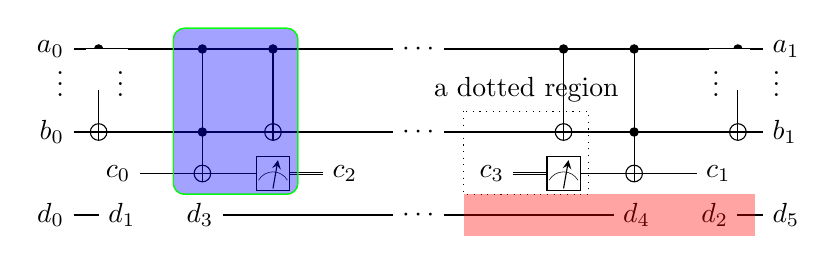
\begin{tikzpicture}[scale=1.000000,x=1pt,y=1pt]
\filldraw[color=white] (0.000000, -7.500000) rectangle (249.000000, 67.500000);
% Drawing wires
% Line 1: a W a_0 a_1
\draw[color=black] (0.000000,60.000000) -- (249.000000,60.000000);
\draw[color=black] (0.000000,60.000000) node[left] {$a_0$};
% Line 2: ...x W
\draw[color=black] (0.000000,45.000000) node[anchor=mid east] {$\vdots$};
% Line 3: b W b_0 b_1
\draw[color=black] (0.000000,30.000000) -- (249.000000,30.000000);
\draw[color=black] (0.000000,30.000000) node[left] {$b_0$};
% Line 4: c W c_0 c_1 c_2 c_3
\draw[color=black] (16.500000,15.000000) -- (72.000000,15.000000);
\draw[color=black] (72.000000,14.500000) -- (97.500000,14.500000);
\draw[color=black] (72.000000,15.500000) -- (97.500000,15.500000);
\draw[color=black] (151.500000,14.500000) -- (177.000000,14.500000);
\draw[color=black] (151.500000,15.500000) -- (177.000000,15.500000);
\draw[color=black] (177.000000,15.000000) -- (232.500000,15.000000);
% Line 5: d W d_0 d_1
\draw[color=black] (0.000000,0.000000) -- (16.500000,0.000000);
\draw[color=black] (46.500000,0.000000) -- (202.500000,0.000000);
\draw[color=black] (232.500000,0.000000) -- (249.000000,0.000000);
\draw[color=black] (0.000000,0.000000) node[left] {$d_0$};
% Done with wires; drawing gates
% Line 10: +b a
\draw (9.000000,60.000000) -- (9.000000,30.000000);
\begin{scope}
\draw[fill=white] (9.000000, 30.000000) circle(3.000000pt);
\clip (9.000000, 30.000000) circle(3.000000pt);
\draw (6.000000, 30.000000) -- (12.000000, 30.000000);
\draw (9.000000, 27.000000) -- (9.000000, 33.000000);
\end{scope}
\filldraw (9.000000, 60.000000) circle(1.500000pt);
\draw (240.000000,60.000000) -- (240.000000,30.000000);
\begin{scope}
\draw[fill=white] (240.000000, 30.000000) circle(3.000000pt);
\clip (240.000000, 30.000000) circle(3.000000pt);
\draw (237.000000, 30.000000) -- (243.000000, 30.000000);
\draw (240.000000, 27.000000) -- (240.000000, 33.000000);
\end{scope}
\filldraw (240.000000, 60.000000) circle(1.500000pt);
% Line 11: c START
\draw[color=black] (24.000000,15.000000) node[fill=white,left,minimum height=15.000000pt,minimum width=15.000000pt,inner sep=0pt] {\phantom{$c_0$}};
\draw[color=black] (24.000000,15.000000) node[left] {$c_0$};
\draw[color=black] (225.000000,15.000000) node[fill=white,right,minimum height=15.000000pt,minimum width=15.000000pt,inner sep=0pt] {\phantom{$c_1$}};
\draw[color=black] (225.000000,15.000000) node[right] {$c_1$};
% Line 12: ...x END
\draw[color=black] (12.000000,45.000000) node[fill=white,right,minimum height=15.000000pt,minimum width=15.000000pt,anchor = base,inner sep=0pt] {\phantom{$\;\vdots\;$}};
\draw[color=black] (12.000000,45.000000) node[anchor=mid west] {$\vdots$};
\draw[color=black] (237.000000,45.000000) node[fill=white,left,minimum height=15.000000pt,minimum width=15.000000pt,anchor = base,inner sep=0pt] {\phantom{$\;\vdots\;$}};
\draw[color=black] (237.000000,45.000000) node[anchor=mid east] {$\vdots$};
% Line 13: d END
\draw[color=black] (9.000000,0.000000) node[fill=white,right,minimum height=15.000000pt,minimum width=15.000000pt,inner sep=0pt] {\phantom{$d_1$}};
\draw[color=black] (9.000000,0.000000) node[right] {$d_1$};
\draw[color=black] (240.000000,0.000000) node[fill=white,left,minimum height=15.000000pt,minimum width=15.000000pt,inner sep=0pt] {\phantom{$d_2$}};
\draw[color=black] (240.000000,0.000000) node[left] {$d_2$};
% Line 14: +c a b
\draw (46.500000,60.000000) -- (46.500000,15.000000);
\begin{scope}
\draw[fill=white] (46.500000, 15.000000) circle(3.000000pt);
\clip (46.500000, 15.000000) circle(3.000000pt);
\draw (43.500000, 15.000000) -- (49.500000, 15.000000);
\draw (46.500000, 12.000000) -- (46.500000, 18.000000);
\end{scope}
\filldraw (46.500000, 60.000000) circle(1.500000pt);
\filldraw (46.500000, 30.000000) circle(1.500000pt);
\draw (202.500000,60.000000) -- (202.500000,15.000000);
\begin{scope}
\draw[fill=white] (202.500000, 15.000000) circle(3.000000pt);
\clip (202.500000, 15.000000) circle(3.000000pt);
\draw (199.500000, 15.000000) -- (205.500000, 15.000000);
\draw (202.500000, 12.000000) -- (202.500000, 18.000000);
\end{scope}
\filldraw (202.500000, 60.000000) circle(1.500000pt);
\filldraw (202.500000, 30.000000) circle(1.500000pt);
% Line 15: d START
\draw[color=black] (54.000000,0.000000) node[fill=white,left,minimum height=15.000000pt,minimum width=15.000000pt,inner sep=0pt] {\phantom{$d_3$}};
\draw[color=black] (54.000000,0.000000) node[left] {$d_3$};
\draw[color=black] (195.000000,0.000000) node[fill=white,right,minimum height=15.000000pt,minimum width=15.000000pt,inner sep=0pt] {\phantom{$d_4$}};
\draw[color=black] (195.000000,0.000000) node[right] {$d_4$};
% Line 16: c M
\draw[fill=white] (66.000000, 9.000000) rectangle (78.000000, 21.000000);
\draw[very thin] (72.000000, 15.600000) arc (90:150:6.000000pt);
\draw[very thin] (72.000000, 15.600000) arc (90:30:6.000000pt);
\draw[->,>=stealth] (72.000000, 9.600000) -- +(80:10.392305pt);
\draw[fill=white] (171.000000, 9.000000) rectangle (183.000000, 21.000000);
\draw[very thin] (177.000000, 15.600000) arc (90:150:6.000000pt);
\draw[very thin] (177.000000, 15.600000) arc (90:30:6.000000pt);
\draw[->,>=stealth] (177.000000, 9.600000) -- +(80:10.392305pt);
% Line 18: +b a
\draw (72.000000,60.000000) -- (72.000000,30.000000);
\begin{scope}
\draw[fill=white] (72.000000, 30.000000) circle(3.000000pt);
\clip (72.000000, 30.000000) circle(3.000000pt);
\draw (69.000000, 30.000000) -- (75.000000, 30.000000);
\draw (72.000000, 27.000000) -- (72.000000, 33.000000);
\end{scope}
\filldraw (72.000000, 60.000000) circle(1.500000pt);
\draw (177.000000,60.000000) -- (177.000000,30.000000);
\begin{scope}
\draw[fill=white] (177.000000, 30.000000) circle(3.000000pt);
\clip (177.000000, 30.000000) circle(3.000000pt);
\draw (174.000000, 30.000000) -- (180.000000, 30.000000);
\draw (177.000000, 27.000000) -- (177.000000, 33.000000);
\end{scope}
\filldraw (177.000000, 60.000000) circle(1.500000pt);
% Line 17: c END
\draw[color=black] (90.000000,15.000000) node[fill=white,right,minimum height=15.000000pt,minimum width=15.000000pt,inner sep=0pt] {\phantom{$c_2$}};
\draw[color=black] (90.000000,15.000000) node[right] {$c_2$};
\draw[color=black] (159.000000,15.000000) node[fill=white,left,minimum height=15.000000pt,minimum width=15.000000pt,inner sep=0pt] {\phantom{$c_3$}};
\draw[color=black] (159.000000,15.000000) node[left] {$c_3$};
% Line 19: LABEL ...
\draw[color=black] (124.500000, 60.000000) node [fill=white] {$\cdots$};
\draw[color=black] (124.500000, 30.000000) node [fill=white] {$\cdots$};
\draw[color=black] (124.500000, 0.000000) node [fill=white] {$\cdots$};
% Done with gates; drawing ending labels
\draw[color=black] (249.000000,60.000000) node[right] {$a_1$};
\draw[color=black] (249.000000,45.000000) node[anchor=mid west] {$\vdots$};
\draw[color=black] (249.000000,30.000000) node[right] {$b_1$};
\draw[color=black] (249.000000,0.000000) node[right] {$d_5$};
% Done with ending labels; drawing cut lines and comments
% Line 21: a c @ 1 2 fill=blue style=rounded_corners color=green
\draw[draw opacity=1.000000,fill opacity=0.200000,color=green,fill=blue,rounded corners] (36.000000,67.500000) rectangle (81.000000,7.500000);
\draw[draw opacity=1.000000,fill opacity=0.200000,color=green,fill=blue,rounded corners] (36.000000,67.500000) rectangle (81.000000,7.500000);
% Line 23: b c @ 5 6 color=black style=dotted % a dotted region
\draw[draw opacity=1.000000,fill opacity=0.200000,color=black,dotted] (141.000000,37.500000) rectangle (186.000000,7.500000);
\draw (163.500000, 37.500000) node[text width=144pt,above,text centered,color=black] {a dotted region};
\draw[draw opacity=1.000000,fill opacity=0.200000,color=black,dotted] (141.000000,37.500000) rectangle (186.000000,7.500000);
% Line 25: d @ 4 fill=red
\draw[draw opacity=0.000000,fill opacity=0.200000,fill=red] (141.000000,7.500000) rectangle (246.000000,-7.500000);
\draw[draw opacity=0.000000,fill opacity=0.200000,fill=red] (141.000000,7.500000) rectangle (246.000000,-7.500000);
% Done with comments
\end{tikzpicture}

\end{figure}

\SaveVerb{name}|starwars|
\begin{figure}[ht]
\caption{\protect\UseVerb{name}}
%! \usetikzlibrary{decorations.pathreplacing,decorations.pathmorphing}
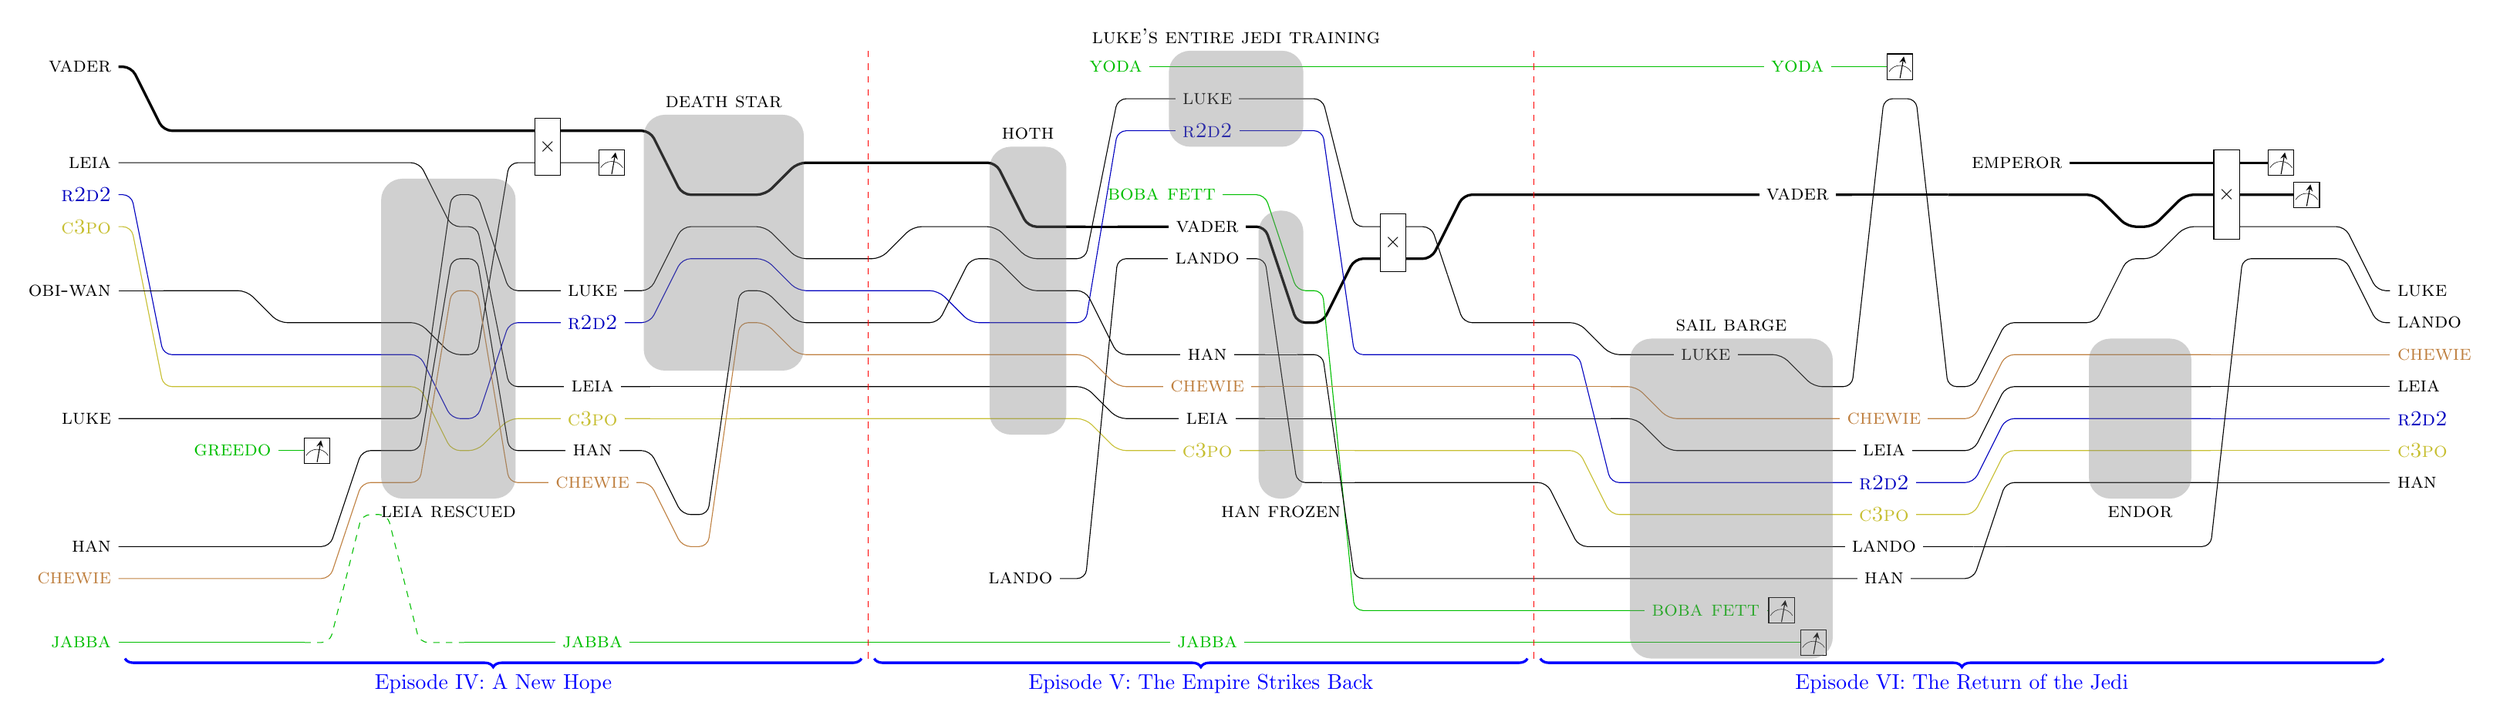
\begin{tikzpicture}[scale=1.000000,x=1pt,y=1pt]
\filldraw[color=white] (0.000000, -7.500000) rectangle (1064.000000, 277.500000);
% Drawing wires
% Line 18: vader W VADER style=very_thick
\draw[color=black,very thick,rounded corners=4.000000pt] (0.000000,270.000000) -- (6.000000,270.000000) -- (13.500000,255.000000);
\draw[color=black,very thick,rounded corners=4.000000pt] (13.500000,255.000000) -- (21.000000,240.000000) -- (249.000000,240.000000) -- (256.500000,225.000000);
\draw[color=black,very thick,rounded corners=4.000000pt] (256.500000,225.000000) -- (264.000000,210.000000) -- (303.000000,210.000000) -- (310.500000,217.500000);
\draw[color=black,very thick,rounded corners=4.000000pt] (310.500000,217.500000) -- (318.000000,225.000000) -- (411.000000,225.000000) -- (418.500000,210.000000);
\draw[color=black,very thick,rounded corners=4.000000pt] (418.500000,210.000000) -- (426.000000,195.000000) -- (453.000000,195.000000);
\draw[color=black,very thick] (453.000000,195.000000) -- (460.500000,195.000000);
\draw[color=black,very thick] (460.500000,195.000000) -- (468.000000,195.000000);
\draw[color=black,very thick,rounded corners=4.000000pt] (468.000000,195.000000) -- (537.000000,195.000000) -- (544.500000,172.500000);
\draw[color=black,very thick,rounded corners=4.000000pt] (544.500000,172.500000) -- (552.000000,150.000000) -- (564.000000,150.000000) -- (571.500000,165.000000);
\draw[color=black,very thick,rounded corners=4.000000pt] (571.500000,165.000000) -- (579.000000,180.000000) -- (615.000000,180.000000) -- (622.500000,195.000000);
\draw[color=black,very thick,rounded corners=4.000000pt] (622.500000,195.000000) -- (630.000000,210.000000) -- (812.000000,210.000000);
\draw[color=black,very thick] (812.000000,210.000000) -- (819.500000,210.000000);
\draw[color=black,very thick] (819.500000,210.000000) -- (827.000000,210.000000);
\draw[color=black,very thick] (827.000000,210.000000) -- (842.000000,210.000000);
\draw[color=black,very thick] (842.000000,210.000000) -- (849.500000,210.000000);
\draw[color=black,very thick] (849.500000,210.000000) -- (857.000000,210.000000);
\draw[color=black,very thick,rounded corners=4.000000pt] (857.000000,210.000000) -- (926.000000,210.000000) -- (933.500000,202.500000);
\draw[color=black,very thick,rounded corners=4.000000pt] (933.500000,202.500000) -- (941.000000,195.000000) -- (953.000000,195.000000) -- (960.500000,202.500000);
\draw[color=black,very thick,rounded corners=4.000000pt] (960.500000,202.500000) -- (968.000000,210.000000) -- (1025.000000,210.000000);
\draw[color=black] (0.000000,270.000000) node[left] {$\textrm{\sc{vader}}$};
% Line 19: boba W BOBA color=green!75!black
\draw[color=green!75!black,rounded corners=4.000000pt] (510.000000,210.000000) -- (537.000000,210.000000) -- (544.500000,187.500000);
\draw[color=green!75!black,rounded corners=4.000000pt] (544.500000,187.500000) -- (552.000000,165.000000) -- (564.000000,165.000000) -- (571.500000,90.000000);
\draw[color=green!75!black,rounded corners=4.000000pt] (571.500000,90.000000) -- (579.000000,15.000000) -- (779.000000,15.000000);
% Line 20: yoda W YODA color=green!75!black
\draw[color=green!75!black] (475.500000,270.000000) -- (834.500000,270.000000);
% Line 21: leia W LEIA LEIA
\draw[color=black,rounded corners=4.000000pt] (0.000000,225.000000) -- (141.000000,225.000000) -- (148.500000,210.000000);
\draw[color=black,rounded corners=4.000000pt] (148.500000,210.000000) -- (156.000000,195.000000) -- (168.000000,195.000000) -- (175.500000,157.500000);
\draw[color=black,rounded corners=4.000000pt] (175.500000,157.500000) -- (183.000000,120.000000) -- (249.000000,120.000000);
\draw[color=black] (249.000000,120.000000) -- (256.500000,120.000000);
\draw[color=black] (256.500000,120.000000) -- (264.000000,120.000000);
\draw[color=black] (264.000000,120.000000) -- (276.000000,120.000000);
\draw[color=black] (276.000000,120.000000) -- (283.500000,120.000000);
\draw[color=black] (283.500000,120.000000) -- (291.000000,120.000000);
\draw[color=black,rounded corners=4.000000pt] (291.000000,120.000000) -- (453.000000,120.000000) -- (460.500000,112.500000);
\draw[color=black,rounded corners=4.000000pt] (460.500000,112.500000) -- (468.000000,105.000000) -- (537.000000,105.000000);
\draw[color=black] (537.000000,105.000000) -- (544.500000,105.000000);
\draw[color=black] (544.500000,105.000000) -- (552.000000,105.000000);
\draw[color=black] (552.000000,105.000000) -- (564.000000,105.000000);
\draw[color=black] (564.000000,105.000000) -- (571.500000,105.000000);
\draw[color=black] (571.500000,105.000000) -- (579.000000,105.000000);
\draw[color=black] (579.000000,105.000000) -- (684.000000,105.000000);
\draw[color=black] (684.000000,105.000000) -- (691.500000,105.000000);
\draw[color=black] (691.500000,105.000000) -- (699.000000,105.000000);
\draw[color=black,rounded corners=4.000000pt] (699.000000,105.000000) -- (711.000000,105.000000) -- (718.500000,97.500000);
\draw[color=black,rounded corners=4.000000pt] (718.500000,97.500000) -- (726.000000,90.000000) -- (869.000000,90.000000) -- (876.500000,105.000000);
\draw[color=black,rounded corners=4.000000pt] (876.500000,105.000000) -- (884.000000,120.000000) -- (980.000000,120.000000);
\draw[color=black] (980.000000,120.000000) -- (987.500000,120.000000);
\draw[color=black] (987.500000,120.000000) -- (995.000000,120.000000);
\draw[color=black] (995.000000,120.000000) -- (1064.000000,120.000000);
\draw[color=black] (0.000000,225.000000) node[left] {$\textrm{\sc{leia}}$};
% Line 22: r2 W R2 R2 color=blue!75!black
\draw[color=blue!75!black,rounded corners=4.000000pt] (0.000000,210.000000) -- (6.000000,210.000000) -- (13.500000,172.500000);
\draw[color=blue!75!black,rounded corners=4.000000pt] (13.500000,172.500000) -- (21.000000,135.000000) -- (141.000000,135.000000) -- (148.500000,120.000000);
\draw[color=blue!75!black,rounded corners=4.000000pt] (148.500000,120.000000) -- (156.000000,105.000000) -- (168.000000,105.000000) -- (175.500000,127.500000);
\draw[color=blue!75!black,rounded corners=4.000000pt] (175.500000,127.500000) -- (183.000000,150.000000) -- (249.000000,150.000000) -- (256.500000,165.000000);
\draw[color=blue!75!black,rounded corners=4.000000pt] (256.500000,165.000000) -- (264.000000,180.000000) -- (303.000000,180.000000) -- (310.500000,172.500000);
\draw[color=blue!75!black,rounded corners=4.000000pt] (310.500000,172.500000) -- (318.000000,165.000000) -- (384.000000,165.000000) -- (391.500000,157.500000);
\draw[color=blue!75!black,rounded corners=4.000000pt] (391.500000,157.500000) -- (399.000000,150.000000) -- (453.000000,150.000000) -- (460.500000,195.000000);
\draw[color=blue!75!black,rounded corners=4.000000pt] (460.500000,195.000000) -- (468.000000,240.000000) -- (564.000000,240.000000) -- (571.500000,187.500000);
\draw[color=blue!75!black,rounded corners=4.000000pt] (571.500000,187.500000) -- (579.000000,135.000000) -- (684.000000,135.000000) -- (691.500000,105.000000);
\draw[color=blue!75!black,rounded corners=4.000000pt] (691.500000,105.000000) -- (699.000000,75.000000) -- (869.000000,75.000000) -- (876.500000,90.000000);
\draw[color=blue!75!black,rounded corners=4.000000pt] (876.500000,90.000000) -- (884.000000,105.000000) -- (980.000000,105.000000);
\draw[color=blue!75!black] (980.000000,105.000000) -- (987.500000,105.000000);
\draw[color=blue!75!black] (987.500000,105.000000) -- (995.000000,105.000000);
\draw[color=blue!75!black] (995.000000,105.000000) -- (1064.000000,105.000000);
\draw[color=blue!75!black] (0.000000,210.000000) node[left] {$\textrm{\sc{r2d2}}$};
% Line 23: c3po W C3PO C3PO color=yellow!75!black
\draw[color=yellow!75!black,rounded corners=4.000000pt] (0.000000,195.000000) -- (6.000000,195.000000) -- (13.500000,157.500000);
\draw[color=yellow!75!black,rounded corners=4.000000pt] (13.500000,157.500000) -- (21.000000,120.000000) -- (141.000000,120.000000) -- (148.500000,105.000000);
\draw[color=yellow!75!black,rounded corners=4.000000pt] (148.500000,105.000000) -- (156.000000,90.000000) -- (168.000000,90.000000) -- (175.500000,97.500000);
\draw[color=yellow!75!black,rounded corners=4.000000pt] (175.500000,97.500000) -- (183.000000,105.000000) -- (249.000000,105.000000);
\draw[color=yellow!75!black] (249.000000,105.000000) -- (256.500000,105.000000);
\draw[color=yellow!75!black] (256.500000,105.000000) -- (264.000000,105.000000);
\draw[color=yellow!75!black] (264.000000,105.000000) -- (276.000000,105.000000);
\draw[color=yellow!75!black] (276.000000,105.000000) -- (283.500000,105.000000);
\draw[color=yellow!75!black] (283.500000,105.000000) -- (291.000000,105.000000);
\draw[color=yellow!75!black,rounded corners=4.000000pt] (291.000000,105.000000) -- (453.000000,105.000000) -- (460.500000,97.500000);
\draw[color=yellow!75!black,rounded corners=4.000000pt] (460.500000,97.500000) -- (468.000000,90.000000) -- (537.000000,90.000000);
\draw[color=yellow!75!black] (537.000000,90.000000) -- (544.500000,90.000000);
\draw[color=yellow!75!black] (544.500000,90.000000) -- (552.000000,90.000000);
\draw[color=yellow!75!black] (552.000000,90.000000) -- (564.000000,90.000000);
\draw[color=yellow!75!black] (564.000000,90.000000) -- (571.500000,90.000000);
\draw[color=yellow!75!black] (571.500000,90.000000) -- (579.000000,90.000000);
\draw[color=yellow!75!black,rounded corners=4.000000pt] (579.000000,90.000000) -- (684.000000,90.000000) -- (691.500000,75.000000);
\draw[color=yellow!75!black,rounded corners=4.000000pt] (691.500000,75.000000) -- (699.000000,60.000000) -- (869.000000,60.000000) -- (876.500000,75.000000);
\draw[color=yellow!75!black,rounded corners=4.000000pt] (876.500000,75.000000) -- (884.000000,90.000000) -- (980.000000,90.000000);
\draw[color=yellow!75!black] (980.000000,90.000000) -- (987.500000,90.000000);
\draw[color=yellow!75!black] (987.500000,90.000000) -- (995.000000,90.000000);
\draw[color=yellow!75!black] (995.000000,90.000000) -- (1064.000000,90.000000);
\draw[color=yellow!75!black] (0.000000,195.000000) node[left] {$\textrm{\sc{c3po}}$};
% Line 24: emperor W EMPEROR style=very_thick
\draw[color=black,very thick] (899.000000,225.000000) -- (1013.000000,225.000000);
% Line 25: ben W BEN
\draw[color=black] (0.000000,165.000000) -- (6.000000,165.000000);
\draw[color=black] (6.000000,165.000000) -- (13.500000,165.000000);
\draw[color=black] (13.500000,165.000000) -- (21.000000,165.000000);
\draw[color=black,rounded corners=4.000000pt] (21.000000,165.000000) -- (60.000000,165.000000) -- (67.500000,157.500000);
\draw[color=black,rounded corners=4.000000pt] (67.500000,157.500000) -- (75.000000,150.000000) -- (141.000000,150.000000) -- (148.500000,142.500000);
\draw[color=black,rounded corners=4.000000pt] (148.500000,142.500000) -- (156.000000,135.000000) -- (168.000000,135.000000) -- (175.500000,180.000000);
\draw[color=black,rounded corners=4.000000pt] (175.500000,180.000000) -- (183.000000,225.000000) -- (231.000000,225.000000);
\draw[color=black] (0.000000,165.000000) node[left] {$\textrm{\sc{obi-wan}}$};
% Line 26: x3 W type=o
% Line 27: x4 W type=o
% Line 28: x5 W type=o
% Line 29: luke W LUKE LUKE
\draw[color=black,rounded corners=4.000000pt] (0.000000,105.000000) -- (141.000000,105.000000) -- (148.500000,157.500000);
\draw[color=black,rounded corners=4.000000pt] (148.500000,157.500000) -- (156.000000,210.000000) -- (168.000000,210.000000) -- (175.500000,187.500000);
\draw[color=black,rounded corners=4.000000pt] (175.500000,187.500000) -- (183.000000,165.000000) -- (249.000000,165.000000) -- (256.500000,180.000000);
\draw[color=black,rounded corners=4.000000pt] (256.500000,180.000000) -- (264.000000,195.000000) -- (303.000000,195.000000) -- (310.500000,187.500000);
\draw[color=black,rounded corners=4.000000pt] (310.500000,187.500000) -- (318.000000,180.000000) -- (357.000000,180.000000) -- (364.500000,187.500000);
\draw[color=black,rounded corners=4.000000pt] (364.500000,187.500000) -- (372.000000,195.000000) -- (411.000000,195.000000) -- (418.500000,187.500000);
\draw[color=black,rounded corners=4.000000pt] (418.500000,187.500000) -- (426.000000,180.000000) -- (453.000000,180.000000) -- (460.500000,217.500000);
\draw[color=black,rounded corners=4.000000pt] (460.500000,217.500000) -- (468.000000,255.000000) -- (564.000000,255.000000) -- (571.500000,225.000000);
\draw[color=black,rounded corners=4.000000pt] (571.500000,225.000000) -- (579.000000,195.000000) -- (615.000000,195.000000) -- (622.500000,172.500000);
\draw[color=black,rounded corners=4.000000pt] (622.500000,172.500000) -- (630.000000,150.000000) -- (684.000000,150.000000) -- (691.500000,142.500000);
\draw[color=black,rounded corners=4.000000pt] (691.500000,142.500000) -- (699.000000,135.000000) -- (779.000000,135.000000) -- (786.500000,127.500000);
\draw[color=black,rounded corners=4.000000pt] (786.500000,127.500000) -- (794.000000,120.000000) -- (812.000000,120.000000) -- (819.500000,187.500000);
\draw[color=black,rounded corners=4.000000pt] (819.500000,187.500000) -- (827.000000,255.000000) -- (842.000000,255.000000) -- (849.500000,187.500000);
\draw[color=black,rounded corners=4.000000pt] (849.500000,187.500000) -- (857.000000,120.000000) -- (869.000000,120.000000) -- (876.500000,135.000000);
\draw[color=black,rounded corners=4.000000pt] (876.500000,135.000000) -- (884.000000,150.000000) -- (926.000000,150.000000) -- (933.500000,165.000000);
\draw[color=black,rounded corners=4.000000pt] (933.500000,165.000000) -- (941.000000,180.000000) -- (953.000000,180.000000) -- (960.500000,187.500000);
\draw[color=black,rounded corners=4.000000pt] (960.500000,187.500000) -- (968.000000,195.000000) -- (1043.000000,195.000000) -- (1050.500000,180.000000);
\draw[color=black,rounded corners=4.000000pt] (1050.500000,180.000000) -- (1058.000000,165.000000) -- (1064.000000,165.000000);
\draw[color=black] (0.000000,105.000000) node[left] {$\textrm{\sc{luke}}$};
% Line 30: greedo W GREEDO color=green!75!black
\draw[color=green!75!black] (67.500000,90.000000) -- (93.000000,90.000000);
% Line 31: x7 W type=o
% Line 32: lando W LANDO LANDO
\draw[color=black,rounded corners=4.000000pt] (433.500000,30.000000) -- (453.000000,30.000000) -- (460.500000,105.000000);
\draw[color=black,rounded corners=4.000000pt] (460.500000,105.000000) -- (468.000000,180.000000) -- (537.000000,180.000000) -- (544.500000,127.500000);
\draw[color=black,rounded corners=4.000000pt] (544.500000,127.500000) -- (552.000000,75.000000) -- (564.000000,75.000000);
\draw[color=black] (564.000000,75.000000) -- (571.500000,75.000000);
\draw[color=black] (571.500000,75.000000) -- (579.000000,75.000000);
\draw[color=black,rounded corners=4.000000pt] (579.000000,75.000000) -- (669.000000,75.000000) -- (676.500000,60.000000);
\draw[color=black,rounded corners=4.000000pt] (676.500000,60.000000) -- (684.000000,45.000000) -- (869.000000,45.000000);
\draw[color=black] (869.000000,45.000000) -- (876.500000,45.000000);
\draw[color=black] (876.500000,45.000000) -- (884.000000,45.000000);
\draw[color=black,rounded corners=4.000000pt] (884.000000,45.000000) -- (980.000000,45.000000) -- (987.500000,112.500000);
\draw[color=black,rounded corners=4.000000pt] (987.500000,112.500000) -- (995.000000,180.000000) -- (1043.000000,180.000000) -- (1050.500000,165.000000);
\draw[color=black,rounded corners=4.000000pt] (1050.500000,165.000000) -- (1058.000000,150.000000) -- (1064.000000,150.000000);
% Line 33: han W HAN HAN
\draw[color=black,rounded corners=4.000000pt] (0.000000,45.000000) -- (99.000000,45.000000) -- (106.500000,67.500000);
\draw[color=black,rounded corners=4.000000pt] (106.500000,67.500000) -- (114.000000,90.000000) -- (141.000000,90.000000) -- (148.500000,135.000000);
\draw[color=black,rounded corners=4.000000pt] (148.500000,135.000000) -- (156.000000,180.000000) -- (168.000000,180.000000) -- (175.500000,135.000000);
\draw[color=black,rounded corners=4.000000pt] (175.500000,135.000000) -- (183.000000,90.000000) -- (249.000000,90.000000) -- (256.500000,75.000000);
\draw[color=black,rounded corners=4.000000pt] (256.500000,75.000000) -- (264.000000,60.000000) -- (276.000000,60.000000) -- (283.500000,112.500000);
\draw[color=black,rounded corners=4.000000pt] (283.500000,112.500000) -- (291.000000,165.000000) -- (303.000000,165.000000) -- (310.500000,157.500000);
\draw[color=black,rounded corners=4.000000pt] (310.500000,157.500000) -- (318.000000,150.000000) -- (384.000000,150.000000) -- (391.500000,165.000000);
\draw[color=black,rounded corners=4.000000pt] (391.500000,165.000000) -- (399.000000,180.000000) -- (411.000000,180.000000) -- (418.500000,172.500000);
\draw[color=black,rounded corners=4.000000pt] (418.500000,172.500000) -- (426.000000,165.000000) -- (453.000000,165.000000) -- (460.500000,150.000000);
\draw[color=black,rounded corners=4.000000pt] (460.500000,150.000000) -- (468.000000,135.000000) -- (537.000000,135.000000);
\draw[color=black] (537.000000,135.000000) -- (544.500000,135.000000);
\draw[color=black] (544.500000,135.000000) -- (552.000000,135.000000);
\draw[color=black,rounded corners=4.000000pt] (552.000000,135.000000) -- (564.000000,135.000000) -- (571.500000,82.500000);
\draw[color=black,rounded corners=4.000000pt] (571.500000,82.500000) -- (579.000000,30.000000) -- (869.000000,30.000000) -- (876.500000,52.500000);
\draw[color=black,rounded corners=4.000000pt] (876.500000,52.500000) -- (884.000000,75.000000) -- (980.000000,75.000000);
\draw[color=black] (980.000000,75.000000) -- (987.500000,75.000000);
\draw[color=black] (987.500000,75.000000) -- (995.000000,75.000000);
\draw[color=black] (995.000000,75.000000) -- (1064.000000,75.000000);
\draw[color=black] (0.000000,45.000000) node[left] {$\textrm{\sc{han}}$};
% Line 34: chewie W CHEWIE CHEWIE color=brown
\draw[color=brown,rounded corners=4.000000pt] (0.000000,30.000000) -- (99.000000,30.000000) -- (106.500000,52.500000);
\draw[color=brown,rounded corners=4.000000pt] (106.500000,52.500000) -- (114.000000,75.000000) -- (141.000000,75.000000) -- (148.500000,120.000000);
\draw[color=brown,rounded corners=4.000000pt] (148.500000,120.000000) -- (156.000000,165.000000) -- (168.000000,165.000000) -- (175.500000,120.000000);
\draw[color=brown,rounded corners=4.000000pt] (175.500000,120.000000) -- (183.000000,75.000000) -- (249.000000,75.000000) -- (256.500000,60.000000);
\draw[color=brown,rounded corners=4.000000pt] (256.500000,60.000000) -- (264.000000,45.000000) -- (276.000000,45.000000) -- (283.500000,97.500000);
\draw[color=brown,rounded corners=4.000000pt] (283.500000,97.500000) -- (291.000000,150.000000) -- (303.000000,150.000000) -- (310.500000,142.500000);
\draw[color=brown,rounded corners=4.000000pt] (310.500000,142.500000) -- (318.000000,135.000000) -- (453.000000,135.000000) -- (460.500000,127.500000);
\draw[color=brown,rounded corners=4.000000pt] (460.500000,127.500000) -- (468.000000,120.000000) -- (537.000000,120.000000);
\draw[color=brown] (537.000000,120.000000) -- (544.500000,120.000000);
\draw[color=brown] (544.500000,120.000000) -- (552.000000,120.000000);
\draw[color=brown] (552.000000,120.000000) -- (564.000000,120.000000);
\draw[color=brown] (564.000000,120.000000) -- (571.500000,120.000000);
\draw[color=brown] (571.500000,120.000000) -- (579.000000,120.000000);
\draw[color=brown] (579.000000,120.000000) -- (684.000000,120.000000);
\draw[color=brown] (684.000000,120.000000) -- (691.500000,120.000000);
\draw[color=brown] (691.500000,120.000000) -- (699.000000,120.000000);
\draw[color=brown,rounded corners=4.000000pt] (699.000000,120.000000) -- (711.000000,120.000000) -- (718.500000,112.500000);
\draw[color=brown,rounded corners=4.000000pt] (718.500000,112.500000) -- (726.000000,105.000000) -- (869.000000,105.000000) -- (876.500000,120.000000);
\draw[color=brown,rounded corners=4.000000pt] (876.500000,120.000000) -- (884.000000,135.000000) -- (980.000000,135.000000);
\draw[color=brown] (980.000000,135.000000) -- (987.500000,135.000000);
\draw[color=brown] (987.500000,135.000000) -- (995.000000,135.000000);
\draw[color=brown] (995.000000,135.000000) -- (1064.000000,135.000000);
\draw[color=brown] (0.000000,30.000000) node[left] {$\textrm{\sc{chewie}}$};
% Line 35: x9 W type=o
% Line 36: jabba W JABBA color=green!75!black
\draw[color=green!75!black] (0.000000,0.000000) -- (87.000000,0.000000);
\draw[color=green!75!black,dashed,rounded corners=4.000000pt] (87.000000,0.000000) -- (99.000000,0.000000) -- (106.500000,30.000000);
\draw[color=green!75!black,dashed,rounded corners=4.000000pt] (106.500000,30.000000) -- (114.000000,60.000000) -- (126.000000,60.000000) -- (133.500000,30.000000);
\draw[color=green!75!black,dashed,rounded corners=4.000000pt] (133.500000,30.000000) -- (141.000000,0.000000) -- (162.000000,0.000000);
\draw[color=green!75!black,solid] (162.000000,0.000000) -- (794.000000,0.000000);
\draw[color=green!75!black] (0.000000,0.000000) node[left] {$\textrm{\sc{jabba}}$};
% Done with wires; drawing gates
% Line 39: x4 x5 r2 c3po PERMUTE
% Line 40: yoda vader PERMUTE
% Line 41: LABEL
% Line 42: greedo START
\draw[color=green!75!black] (75.000000,90.000000) node[fill=white,left,minimum height=15.000000pt,minimum width=15.000000pt,inner sep=0pt] {\phantom{$\textrm{\sc{greedo}}$}};
\draw[color=green!75!black] (75.000000,90.000000) node[left] {$\textrm{\sc{greedo}}$};
% Line 43: x3 ben PERMUTE
% Line 45: greedo:type=o M
\draw[fill=white] (87.000000, 84.000000) rectangle (99.000000, 96.000000);
\draw[very thin] (93.000000, 90.600000) arc (90:150:6.000000pt);
\draw[very thin] (93.000000, 90.600000) arc (90:30:6.000000pt);
\draw[->,>=stealth] (93.000000, 84.600000) -- +(80:10.392305pt);
% Line 46: jabba:style=dashed LABEL length=0
% Line 47: han chewie jabba greedo x7 lando x9 PERMUTE
% Line 49: x7 lando x9 jabba PERMUTE
% Line 50: x4 luke leia han chewie x5 ben emperor r2 c3po x3 PERMUTE
% Line 51: jabba:style=solid TOUCH
% Line 52: ben x4 x5 x3 luke r2 emperor leia c3po han chewie PERMUTE
% Line 55: vader ben DUEL
\draw (201.000000,240.000000) -- (201.000000,225.000000);
\begin{scope}
\draw[fill=white] (201.000000, 232.500000) +(-45.000000:8.485281pt and 19.091883pt) -- +(45.000000:8.485281pt and 19.091883pt) -- +(135.000000:8.485281pt and 19.091883pt) -- +(225.000000:8.485281pt and 19.091883pt) -- cycle;
\clip (201.000000, 232.500000) +(-45.000000:8.485281pt and 19.091883pt) -- +(45.000000:8.485281pt and 19.091883pt) -- +(135.000000:8.485281pt and 19.091883pt) -- +(225.000000:8.485281pt and 19.091883pt) -- cycle;
\draw (201.000000, 232.500000) node {$\times$};
\end{scope}
% Line 56: ben LABEL length=18
% Line 57: ben:type=o M
\draw[fill=white] (225.000000, 219.000000) rectangle (237.000000, 231.000000);
\draw[very thin] (231.000000, 225.600000) arc (90:150:6.000000pt);
\draw[very thin] (231.000000, 225.600000) arc (90:30:6.000000pt);
\draw[->,>=stealth] (231.000000, 219.600000) -- +(80:10.392305pt);
% Line 58: luke leia han c3po r2 chewie jabba LABEL length=30 LUKE LEIA HAN C3PO R2 CHEWIE JABBA
\draw[color=black] (222.000000, 165.000000) node [fill=white] {$\textrm{\sc{luke}}$};
\draw[color=black] (222.000000, 120.000000) node [fill=white] {$\textrm{\sc{leia}}$};
\draw[color=black] (222.000000, 90.000000) node [fill=white] {$\textrm{\sc{han}}$};
\draw[color=yellow!75!black] (222.000000, 105.000000) node [fill=white] {$\textrm{\sc{c3po}}$};
\draw[color=blue!75!black] (222.000000, 150.000000) node [fill=white] {$\textrm{\sc{r2d2}}$};
\draw[color=brown] (222.000000, 75.000000) node [fill=white] {$\textrm{\sc{chewie}}$};
\draw[color=green!75!black] (222.000000, 0.000000) node [fill=white] {$\textrm{\sc{jabba}}$};
% Line 60: ben x4 vader luke r2 x5 x3 emperor leia c3po x7 greedo han chewie PERMUTE
% Line 61: han chewie x5 x3 PERMUTE
% Line 62: vader x4 emperor luke r2 han chewie PERMUTE
% Line 64: LABEL
% Line 66: luke emperor PERMUTE
% Line 67: han emperor r2 PERMUTE
% Line 68: x4 emperor vader luke han PERMUTE
% Line 70: lando START
\draw[color=black] (441.000000,30.000000) node[fill=white,left,minimum height=15.000000pt,minimum width=15.000000pt,inner sep=0pt] {\phantom{$\textrm{\sc{lando}}$}};
\draw[color=black] (441.000000,30.000000) node[left] {$\textrm{\sc{lando}}$};
% Line 72: luke r2 ben boba vader lando x4 emperor han chewie leia c3po x7 greedo x5 x3 PERMUTE
% Line 73: yoda START
\draw[color=green!75!black] (483.000000,270.000000) node[fill=white,left,minimum height=15.000000pt,minimum width=15.000000pt,inner sep=0pt] {\phantom{$\textrm{\sc{yoda}}$}};
\draw[color=green!75!black] (483.000000,270.000000) node[left] {$\textrm{\sc{yoda}}$};
% Line 74: vader luke leia han c3po r2 chewie jabba lando LABEL length=30 VADER LUKE LEIA HAN C3PO R2 CHEWIE JABBA LANDO
\draw[color=black] (510.000000, 195.000000) node [fill=white] {$\textrm{\sc{vader}}$};
\draw[color=black] (510.000000, 255.000000) node [fill=white] {$\textrm{\sc{luke}}$};
\draw[color=black] (510.000000, 105.000000) node [fill=white] {$\textrm{\sc{leia}}$};
\draw[color=black] (510.000000, 135.000000) node [fill=white] {$\textrm{\sc{han}}$};
\draw[color=yellow!75!black] (510.000000, 90.000000) node [fill=white] {$\textrm{\sc{c3po}}$};
\draw[color=blue!75!black] (510.000000, 240.000000) node [fill=white] {$\textrm{\sc{r2d2}}$};
\draw[color=brown] (510.000000, 120.000000) node [fill=white] {$\textrm{\sc{chewie}}$};
\draw[color=green!75!black] (510.000000, 0.000000) node [fill=white] {$\textrm{\sc{jabba}}$};
\draw[color=black] (510.000000, 180.000000) node [fill=white] {$\textrm{\sc{lando}}$};
% Line 75: boba START
\draw[color=green!75!black] (517.500000,210.000000) node[fill=white,left,minimum height=15.000000pt,minimum width=15.000000pt,inner sep=0pt] {\phantom{$\textrm{\sc{boba fett}}$}};
\draw[color=green!75!black] (517.500000,210.000000) node[left] {$\textrm{\sc{boba fett}}$};
% Line 76: x4 emperor x7 boba vader han chewie leia c3po lando PERMUTE
% Line 79: ben x4 emperor x7 luke vader x5 greedo r2 chewie leia c3po lando  x3 x9 han boba PERMUTE
% Line 80: vader luke DUEL
\draw (597.000000,195.000000) -- (597.000000,180.000000);
\begin{scope}
\draw[fill=white] (597.000000, 187.500000) +(-45.000000:8.485281pt and 19.091883pt) -- +(45.000000:8.485281pt and 19.091883pt) -- +(135.000000:8.485281pt and 19.091883pt) -- +(225.000000:8.485281pt and 19.091883pt) -- cycle;
\clip (597.000000, 187.500000) +(-45.000000:8.485281pt and 19.091883pt) -- +(45.000000:8.485281pt and 19.091883pt) -- +(135.000000:8.485281pt and 19.091883pt) -- +(225.000000:8.485281pt and 19.091883pt) -- cycle;
\draw (597.000000, 187.500000) node {$\times$};
\end{scope}
% Line 81: vader x7 x5 greedo luke PERMUTE
% Line 82: LABEL
% Line 85: x3 x9 lando PERMUTE
% Line 86: x3 luke chewie leia x9 r2 c3po PERMUTE
% Line 90: x9 chewie leia PERMUTE
% Line 91: luke boba LABEL LUKE BOBA length=35
\draw[color=black] (743.500000, 135.000000) node [fill=white] {$\textrm{\sc{luke}}$};
\draw[color=green!75!black] (743.500000, 15.000000) node [fill=white] {$\textrm{\sc{boba fett}}$};
% Line 94: yoda vader LABEL YODA VADER
\draw[color=green!75!black] (786.500000, 270.000000) node [fill=white] {$\textrm{\sc{yoda}}$};
\draw[color=black] (786.500000, 210.000000) node [fill=white] {$\textrm{\sc{vader}}$};
% Line 95: x9 luke PERMUTE
% Line 96: boba:type=0 M
\draw[fill=white] (773.000000, 9.000000) rectangle (785.000000, 21.000000);
\draw[very thin] (779.000000, 15.600000) arc (90:150:6.000000pt);
\draw[very thin] (779.000000, 15.600000) arc (90:30:6.000000pt);
\draw[->,>=stealth] (779.000000, 9.600000) -- +(80:10.392305pt);
% Line 97: boba jabba PHANTOM
% Line 98: jabba:type=0 M
\draw[fill=white] (788.000000, -6.000000) rectangle (800.000000, 6.000000);
\draw[very thin] (794.000000, 0.600000) arc (90:150:6.000000pt);
\draw[very thin] (794.000000, 0.600000) arc (90:30:6.000000pt);
\draw[->,>=stealth] (794.000000, -5.400000) -- +(80:10.392305pt);
% Line 102: luke ben PERMUTE
% Line 103: yoda:type=0 M
\draw[fill=white] (828.500000, 264.000000) rectangle (840.500000, 276.000000);
\draw[very thin] (834.500000, 270.600000) arc (90:150:6.000000pt);
\draw[very thin] (834.500000, 270.600000) arc (90:30:6.000000pt);
\draw[->,>=stealth] (834.500000, 264.600000) -- +(80:10.392305pt);
% Line 104: leia han c3po r2 chewie jabba lando LABEL length=30 LEIA HAN C3PO R2 CHEWIE JABBA LANDO
\draw[color=black] (827.000000, 90.000000) node [fill=white] {$\textrm{\sc{leia}}$};
\draw[color=black] (827.000000, 30.000000) node [fill=white] {$\textrm{\sc{han}}$};
\draw[color=yellow!75!black] (827.000000, 60.000000) node [fill=white] {$\textrm{\sc{c3po}}$};
\draw[color=blue!75!black] (827.000000, 75.000000) node [fill=white] {$\textrm{\sc{r2d2}}$};
\draw[color=brown] (827.000000, 105.000000) node [fill=white] {$\textrm{\sc{chewie}}$};
\draw[color=black] (827.000000, 45.000000) node [fill=white] {$\textrm{\sc{lando}}$};
% Line 105: ben luke PERMUTE
% Line 107: luke chewie leia r2 c3po han x3 x9 PERMUTE
% Line 108: emperor START length=30
\draw[color=black] (914.000000,225.000000) node[fill=white,left,minimum height=15.000000pt,minimum width=30.000000pt,inner sep=0pt] {\phantom{$\textrm{\sc{emperor}}$}};
\draw[color=black] (914.000000,225.000000) node[left] {$\textrm{\sc{emperor}}$};
% Line 109: x7 vader luke x5 greedo PERMUTE
% Line 110: vader luke x7 PERMUTE
% Line 113: emperor vader luke DUEL
\draw (987.500000,225.000000) -- (987.500000,195.000000);
\begin{scope}
\draw[fill=white] (987.500000, 210.000000) +(-45.000000:8.485281pt and 29.698485pt) -- +(45.000000:8.485281pt and 29.698485pt) -- +(135.000000:8.485281pt and 29.698485pt) -- +(225.000000:8.485281pt and 29.698485pt) -- cycle;
\clip (987.500000, 210.000000) +(-45.000000:8.485281pt and 29.698485pt) -- +(45.000000:8.485281pt and 29.698485pt) -- +(135.000000:8.485281pt and 29.698485pt) -- +(225.000000:8.485281pt and 29.698485pt) -- cycle;
\draw (987.500000, 210.000000) node {$\times$};
\end{scope}
% Line 114: lando x7 PERMUTE
% Line 117: emperor:type=0 M
\draw[fill=white] (1007.000000, 219.000000) rectangle (1019.000000, 231.000000);
\draw[very thin] (1013.000000, 225.600000) arc (90:150:6.000000pt);
\draw[very thin] (1013.000000, 225.600000) arc (90:30:6.000000pt);
\draw[->,>=stealth] (1013.000000, 219.600000) -- +(80:10.392305pt);
% Line 118: emperor vader PHANTOM
% Line 119: vader:type=0 M
\draw[fill=white] (1019.000000, 204.000000) rectangle (1031.000000, 216.000000);
\draw[very thin] (1025.000000, 210.600000) arc (90:150:6.000000pt);
\draw[very thin] (1025.000000, 210.600000) arc (90:30:6.000000pt);
\draw[->,>=stealth] (1025.000000, 204.600000) -- +(80:10.392305pt);
% Line 121: TOUCH
% Line 122: x5 greedo luke lando PERMUTE
% Done with gates; drawing ending labels
\draw[color=black] (1064.000000,120.000000) node[right] {$\textrm{\sc{leia}}$};
\draw[color=blue!75!black] (1064.000000,105.000000) node[right] {$\textrm{\sc{r2d2}}$};
\draw[color=yellow!75!black] (1064.000000,90.000000) node[right] {$\textrm{\sc{c3po}}$};
\draw[color=black] (1064.000000,165.000000) node[right] {$\textrm{\sc{luke}}$};
\draw[color=black] (1064.000000,150.000000) node[right] {$\textrm{\sc{lando}}$};
\draw[color=black] (1064.000000,75.000000) node[right] {$\textrm{\sc{han}}$};
\draw[color=brown] (1064.000000,135.000000) node[right] {$\textrm{\sc{chewie}}$};
% Done with ending labels; drawing cut lines and comments
\draw[dashed,color=red] (351.000000, -7.500000) -- (351.000000, 277.500000);
\draw[dashed,color=red] (663.000000, -7.500000) -- (663.000000, 277.500000);
% Line 53: chewie x4 @ 2 fill=gray style=rounded_corners=10pt %% {\sc leia rescued}
\draw[draw opacity=0.000000,fill opacity=0.200000,fill=gray,rounded corners=10pt] (123.000000,217.500000) rectangle (186.000000,67.500000);
\draw (154.500000, 67.500000) node[text width=288.0pt,below,text centered] {{\sc leia rescued}};
\draw[draw opacity=0.000000,fill opacity=0.200000,fill=gray,rounded corners=10pt] (123.000000,217.500000) rectangle (186.000000,67.500000);
% Line 63: vader emperor @ 3 fill=gray style=rounded_corners=10pt % {\sc death star}
\draw[draw opacity=0.000000,fill opacity=0.200000,fill=gray,rounded corners=10pt] (246.000000,247.500000) rectangle (321.000000,127.500000);
\draw (283.500000, 247.500000) node[text width=288.0pt,above,text centered] {{\sc death star}};
\draw[draw opacity=0.000000,fill opacity=0.200000,fill=gray,rounded corners=10pt] (246.000000,247.500000) rectangle (321.000000,127.500000);
% Line 69: vader c3po @ 1 fill=gray style=rounded_corners=10pt % {\sc hoth}
\draw[draw opacity=0.000000,fill opacity=0.200000,fill=gray,rounded corners=10pt] (408.000000,232.500000) rectangle (444.000000,97.500000);
\draw (426.000000, 232.500000) node[text width=288.0pt,above,text centered] {{\sc hoth}};
\draw[draw opacity=0.000000,fill opacity=0.200000,fill=gray,rounded corners=10pt] (408.000000,232.500000) rectangle (444.000000,97.500000);
% Line 77: yoda r2 @ 2 fill=gray style=rounded_corners=10pt % {\sc luke's entire jedi training}
\draw[draw opacity=0.000000,fill opacity=0.200000,fill=gray,rounded corners=10pt] (492.000000,277.500000) rectangle (555.000000,232.500000);
\draw (523.500000, 277.500000) node[text width=288.0pt,above,text centered] {{\sc luke's entire jedi training}};
\draw[draw opacity=0.000000,fill opacity=0.200000,fill=gray,rounded corners=10pt] (492.000000,277.500000) rectangle (555.000000,232.500000);
% Line 78: vader x7 @ 1 fill=gray style=rounded_corners=10pt %% {\sc han frozen}
\draw[draw opacity=0.000000,fill opacity=0.200000,fill=gray,rounded corners=10pt] (534.000000,202.500000) rectangle (555.000000,67.500000);
\draw (544.500000, 67.500000) node[text width=288.0pt,below,text centered] {{\sc han frozen}};
\draw[draw opacity=0.000000,fill opacity=0.200000,fill=gray,rounded corners=10pt] (534.000000,202.500000) rectangle (555.000000,67.500000);
% Line 100: luke jabba @ 2 fill=gray style=rounded_corners=10pt % {\sc sail barge}
\draw[draw opacity=0.000000,fill opacity=0.200000,fill=gray,rounded corners=10pt] (708.000000,142.500000) rectangle (803.000000,-7.500000);
\draw (755.500000, 142.500000) node[text width=288.0pt,above,text centered] {{\sc sail barge}};
\draw[draw opacity=0.000000,fill opacity=0.200000,fill=gray,rounded corners=10pt] (708.000000,142.500000) rectangle (803.000000,-7.500000);
% Line 111: chewie han @ 2  fill=gray style=rounded_corners=10pt %% {\sc endor}
\draw[draw opacity=0.000000,fill opacity=0.200000,fill=gray,rounded corners=10pt] (923.000000,142.500000) rectangle (971.000000,67.500000);
\draw (947.000000, 67.500000) node[text width=288.0pt,below,text centered] {{\sc endor}};
\draw[draw opacity=0.000000,fill opacity=0.200000,fill=gray,rounded corners=10pt] (923.000000,142.500000) rectangle (971.000000,67.500000);
% Line 123: @ 0 start5 color=blue %% Episode IV: A New Hope
\draw[decorate,decoration={brace,mirror,amplitude = 4.000000pt},very thick,color=blue] (3.000000,-7.500000) -- (348.000000,-7.500000);
\draw (175.500000, -11.500000) node[text width=288.0pt,below,text centered,color=blue] {Episode IV: A New Hope};
% Line 124: @ start5 start6 color=blue %% Episode V: The Empire Strikes Back
\draw[decorate,decoration={brace,mirror,amplitude = 4.000000pt},very thick,color=blue] (354.000000,-7.500000) -- (660.000000,-7.500000);
\draw (507.000000, -11.500000) node[text width=288.0pt,below,text centered,color=blue] {Episode V: The Empire Strikes Back};
% Line 125: @ start6 color=blue %% Episode VI: The Return of the Jedi
\draw[decorate,decoration={brace,mirror,amplitude = 4.000000pt},very thick,color=blue] (666.000000,-7.500000) -- (1061.000000,-7.500000);
\draw (863.500000, -11.500000) node[text width=288.0pt,below,text centered,color=blue] {Episode VI: The Return of the Jedi};
% Done with comments
\end{tikzpicture}

\end{figure}

\SaveVerb{name}|test-rotate|
\begin{figure}[ht]
\caption{\protect\UseVerb{name}}
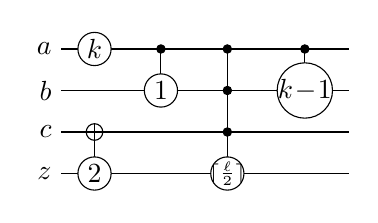
\begin{tikzpicture}[scale=1.000000,x=1pt,y=1pt]
\filldraw[color=white] (0.000000, -7.500000) rectangle (104.000000, 52.500000);
% Drawing wires
% Line 1: a W a
\draw[color=black] (0.000000,45.000000) -- (104.000000,45.000000);
\draw[color=black] (0.000000,45.000000) node[left] {$a$};
% Line 2: b W b
\draw[color=black] (0.000000,30.000000) -- (104.000000,30.000000);
\draw[color=black] (0.000000,30.000000) node[left] {$b$};
% Line 3: c W c
\draw[color=black] (0.000000,15.000000) -- (104.000000,15.000000);
\draw[color=black] (0.000000,15.000000) node[left] {$c$};
% Line 4: k W z
\draw[color=black] (0.000000,0.000000) -- (104.000000,0.000000);
\draw[color=black] (0.000000,0.000000) node[left] {$z$};
% Done with wires; drawing gates
% Line 8: a P $k$
\begin{scope}
\draw[fill=white] (12.000000, 45.000000) circle(6.000000pt);
\clip (12.000000, 45.000000) circle(6.000000pt);
\draw (12.000000, 45.000000) node {$k$};
\end{scope}
% Line 10: k P 2 +c
\draw (12.000000,15.000000) -- (12.000000,0.000000);
\begin{scope}
\draw[fill=white] (12.000000, 0.000000) circle(6.000000pt);
\clip (12.000000, 0.000000) circle(6.000000pt);
\draw (12.000000, 0.000000) node {2};
\end{scope}
\begin{scope}
\draw[fill=white] (12.000000, 15.000000) circle(3.000000pt);
\clip (12.000000, 15.000000) circle(3.000000pt);
\draw (9.000000, 15.000000) -- (15.000000, 15.000000);
\draw (12.000000, 12.000000) -- (12.000000, 18.000000);
\end{scope}
% Line 9: b P 1 a
\draw (36.000000,45.000000) -- (36.000000,30.000000);
\begin{scope}
\draw[fill=white] (36.000000, 30.000000) circle(6.000000pt);
\clip (36.000000, 30.000000) circle(6.000000pt);
\draw (36.000000, 30.000000) node {1};
\end{scope}
\filldraw (36.000000, 45.000000) circle(1.500000pt);
% Line 11: k P $\scriptstyle\lceil\frac\ell2\rceil$ a b c
\draw (60.000000,45.000000) -- (60.000000,0.000000);
\begin{scope}
\draw[fill=white] (60.000000, 0.000000) circle(6.000000pt);
\clip (60.000000, 0.000000) circle(6.000000pt);
\draw (60.000000, 0.000000) node {$\scriptstyle\lceil\frac\ell2\rceil$};
\end{scope}
\filldraw (60.000000, 45.000000) circle(1.500000pt);
\filldraw (60.000000, 30.000000) circle(1.500000pt);
\filldraw (60.000000, 15.000000) circle(1.500000pt);
% Line 12: b Pk1 a
\draw (88.000000,45.000000) -- (88.000000,30.000000);
\begin{scope}
\draw[fill=white] (88.000000, 30.000000) circle(10.000000pt);
\clip (88.000000, 30.000000) circle(10.000000pt);
\draw (88.000000, 30.000000) node {$k\!-\!1$};
\end{scope}
\filldraw (88.000000, 45.000000) circle(1.500000pt);
% Done with gates; drawing ending labels
% Done with ending labels; drawing cut lines and comments
% Done with comments
\end{tikzpicture}

\end{figure}

\SaveVerb{name}|test40|
\begin{figure}[ht]
\caption{\protect\UseVerb{name}}
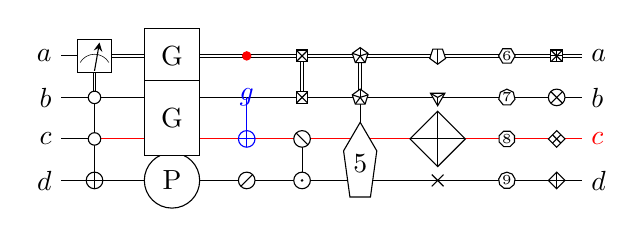
\begin{tikzpicture}[scale=1.000000,x=1pt,y=1pt]
\filldraw[color=white] (0.000000, -7.500000) rectangle (188.000000, 52.500000);
% Drawing wires
% Line 1: a W a a
\draw[color=black] (0.000000,45.000000) -- (12.000000,45.000000);
\draw[color=black] (12.000000,44.500000) -- (188.000000,44.500000);
\draw[color=black] (12.000000,45.500000) -- (188.000000,45.500000);
\draw[color=black] (0.000000,45.000000) node[left] {$a$};
% Line 2: b W b b
\draw[color=black] (0.000000,30.000000) -- (188.000000,30.000000);
\draw[color=black] (0.000000,30.000000) node[left] {$b$};
% Line 3: c W c c
\draw[color=black] (0.000000,15.000000) -- (12.000000,15.000000);
\draw[color=red] (12.000000,15.000000) -- (188.000000,15.000000);
\draw[color=black] (0.000000,15.000000) node[left] {$c$};
% Line 4: d W d d
\draw[color=black] (0.000000,0.000000) -- (188.000000,0.000000);
\draw[color=black] (0.000000,0.000000) node[left] {$d$};
% Done with wires; drawing gates
% Line 6: +d a:cwire -b -c:color=red
\draw (11.500000,45.000000) -- (11.500000,30.000000);
\draw (12.500000,45.000000) -- (12.500000,30.000000);
\draw (12.000000,30.000000) -- (12.000000,0.000000);
\begin{scope}
\draw[fill=white] (12.000000, 0.000000) circle(3.000000pt);
\clip (12.000000, 0.000000) circle(3.000000pt);
\draw (9.000000, 0.000000) -- (15.000000, 0.000000);
\draw (12.000000, -3.000000) -- (12.000000, 3.000000);
\end{scope}
\filldraw (12.000000, 45.000000) circle(1.500000pt);
\draw[fill=white] (12.000000, 30.000000) circle(2.250000pt);
\draw[fill=white] (12.000000, 15.000000) circle(2.250000pt);
\draw[fill=white] (6.000000, 39.000000) rectangle (18.000000, 51.000000);
\draw[very thin] (12.000000, 45.600000) arc (90:150:6.000000pt);
\draw[very thin] (12.000000, 45.600000) arc (90:30:6.000000pt);
\draw[->,>=stealth] (12.000000, 39.600000) -- +(80:10.392305pt);
% Line 8: d P P size=20
\begin{scope}
\draw[fill=white] (40.000000, 0.000000) circle(10.000000pt);
\clip (40.000000, 0.000000) circle(10.000000pt);
\draw (40.000000, 0.000000) node {P};
\end{scope}
% Line 9: a G G si=20
\begin{scope}
\draw[fill=white] (40.000000, 45.000000) +(-45.000000:14.142136pt and 14.142136pt) -- +(45.000000:14.142136pt and 14.142136pt) -- +(135.000000:14.142136pt and 14.142136pt) -- +(225.000000:14.142136pt and 14.142136pt) -- cycle;
\clip (40.000000, 45.000000) +(-45.000000:14.142136pt and 14.142136pt) -- +(45.000000:14.142136pt and 14.142136pt) -- +(135.000000:14.142136pt and 14.142136pt) -- +(225.000000:14.142136pt and 14.142136pt) -- cycle;
\draw (40.000000, 45.000000) node {G};
\end{scope}
% Line 10: b c G G size=20
\draw (40.000000,30.000000) -- (40.000000,15.000000);
\begin{scope}
\draw[fill=white] (40.000000, 22.500000) +(-45.000000:14.142136pt and 19.091883pt) -- +(45.000000:14.142136pt and 19.091883pt) -- +(135.000000:14.142136pt and 19.091883pt) -- +(225.000000:14.142136pt and 19.091883pt) -- cycle;
\clip (40.000000, 22.500000) +(-45.000000:14.142136pt and 19.091883pt) -- +(45.000000:14.142136pt and 19.091883pt) -- +(135.000000:14.142136pt and 19.091883pt) -- +(225.000000:14.142136pt and 19.091883pt) -- cycle;
\draw (40.000000, 22.500000) node {G};
\end{scope}
% Line 12: a shape=3:size=10:color=red
\begin{scope}[color=red]
\filldraw (67.000000, 45.000000) circle(1.500000pt);
\end{scope}
% Line 14: b:shape=0:operator=$g$ color=blue +c
\begin{scope}[color=blue]
\draw (67.000000,30.000000) -- (67.000000,15.000000);
\begin{scope}
\draw (67.000000, 30.000000) node {$g$};
\end{scope}
\begin{scope}
\draw[fill=white] (67.000000, 15.000000) circle(3.000000pt);
\clip (67.000000, 15.000000) circle(3.000000pt);
\draw (64.000000, 15.000000) -- (70.000000, 15.000000);
\draw (67.000000, 12.000000) -- (67.000000, 18.000000);
\end{scope}
\end{scope}
% Line 16: +d:operator=/
\begin{scope}
\draw[fill=white] (67.000000, 0.000000) circle(3.000000pt);
\clip (67.000000, 0.000000) circle(3.000000pt);
\draw (64.878680, -2.121320) -- (69.121320, 2.121320);
\end{scope}
% Line 18: +a +b operator=x shape=box
\draw (86.500000,45.000000) -- (86.500000,30.000000);
\draw (87.500000,45.000000) -- (87.500000,30.000000);
\begin{scope}
\draw[fill=white] (87.000000, 45.000000) +(-45.000000:3.000000pt) -- +(45.000000:3.000000pt) -- +(135.000000:3.000000pt) -- +(225.000000:3.000000pt) -- cycle;
\clip (87.000000, 45.000000) +(-45.000000:3.000000pt) -- +(45.000000:3.000000pt) -- +(135.000000:3.000000pt) -- +(225.000000:3.000000pt) -- cycle;
\draw (84.878680, 42.878680) -- (89.121320, 47.121320);
\draw (84.878680, 47.121320) -- (89.121320, 42.878680);
\end{scope}
\begin{scope}
\draw[fill=white] (87.000000, 30.000000) +(-45.000000:3.000000pt) -- +(45.000000:3.000000pt) -- +(135.000000:3.000000pt) -- +(225.000000:3.000000pt) -- cycle;
\clip (87.000000, 30.000000) +(-45.000000:3.000000pt) -- +(45.000000:3.000000pt) -- +(135.000000:3.000000pt) -- +(225.000000:3.000000pt) -- cycle;
\draw (84.878680, 27.878680) -- (89.121320, 32.121320);
\draw (84.878680, 32.121320) -- (89.121320, 27.878680);
\end{scope}
% Line 20: +c:operator=\\ +d:operator=.
\draw (87.000000,15.000000) -- (87.000000,0.000000);
\begin{scope}
\draw[fill=white] (87.000000, 15.000000) circle(3.000000pt);
\clip (87.000000, 15.000000) circle(3.000000pt);
\draw (84.878680, 17.121320) -- (89.121320, 12.878680);
\end{scope}
\begin{scope}
\draw[fill=white] (87.000000, 0.000000) circle(3.000000pt);
\clip (87.000000, 0.000000) circle(3.000000pt);
\filldraw (87.000000, 0.000000) circle(0.250000pt);
\end{scope}
% Line 22: c d G:op=5 +a +b operator=* shape=5
\draw (107.500000,45.000000) -- (107.500000,30.000000);
\draw (108.500000,45.000000) -- (108.500000,30.000000);
\draw (108.000000,30.000000) -- (108.000000,0.000000);
\begin{scope}
\draw[fill=white] (108.000000, 6.074767) +(-54.000000:6.308773pt and 14.925233pt) -- +(18.000000:6.308773pt and 14.925233pt) -- +(90.000000:6.308773pt and 14.925233pt) -- +(162.000000:6.308773pt and 14.925233pt) -- +(234.000000:6.308773pt and 14.925233pt) -- cycle;
\clip (108.000000, 6.074767) +(-54.000000:6.308773pt and 14.925233pt) -- +(18.000000:6.308773pt and 14.925233pt) -- +(90.000000:6.308773pt and 14.925233pt) -- +(162.000000:6.308773pt and 14.925233pt) -- +(234.000000:6.308773pt and 14.925233pt) -- cycle;
\draw (108.000000, 6.074767) node {5};
\end{scope}
\begin{scope}
\draw[fill=white] (108.000000, 45.000000) +(-54.000000:3.000000pt) -- +(18.000000:3.000000pt) -- +(90.000000:3.000000pt) -- +(162.000000:3.000000pt) -- +(234.000000:3.000000pt) -- cycle;
\clip (108.000000, 45.000000) +(-54.000000:3.000000pt) -- +(18.000000:3.000000pt) -- +(90.000000:3.000000pt) -- +(162.000000:3.000000pt) -- +(234.000000:3.000000pt) -- cycle;
\draw (108.000000, 45.000000) -- +(-54.000000:3.000000pt);
\draw (108.000000, 45.000000) -- +(18.000000:3.000000pt);
\draw (108.000000, 45.000000) -- +(90.000000:3.000000pt);
\draw (108.000000, 45.000000) -- +(162.000000:3.000000pt);
\draw (108.000000, 45.000000) -- +(234.000000:3.000000pt);
\end{scope}
\begin{scope}
\draw[fill=white] (108.000000, 30.000000) +(-54.000000:3.000000pt) -- +(18.000000:3.000000pt) -- +(90.000000:3.000000pt) -- +(162.000000:3.000000pt) -- +(234.000000:3.000000pt) -- cycle;
\clip (108.000000, 30.000000) +(-54.000000:3.000000pt) -- +(18.000000:3.000000pt) -- +(90.000000:3.000000pt) -- +(162.000000:3.000000pt) -- +(234.000000:3.000000pt) -- cycle;
\draw (108.000000, 30.000000) -- +(-54.000000:3.000000pt);
\draw (108.000000, 30.000000) -- +(18.000000:3.000000pt);
\draw (108.000000, 30.000000) -- +(90.000000:3.000000pt);
\draw (108.000000, 30.000000) -- +(162.000000:3.000000pt);
\draw (108.000000, 30.000000) -- +(234.000000:3.000000pt);
\end{scope}
% Line 24: c:shape=-4:size=20
\begin{scope}
\draw[fill=white] (136.000000, 15.000000) +(-90.000000:10.000000pt) -- +(0.000000:10.000000pt) -- +(90.000000:10.000000pt) -- +(180.000000:10.000000pt) -- cycle;
\clip (136.000000, 15.000000) +(-90.000000:10.000000pt) -- +(0.000000:10.000000pt) -- +(90.000000:10.000000pt) -- +(180.000000:10.000000pt) -- cycle;
\draw (126.000000, 15.000000) -- (146.000000, 15.000000);
\draw (136.000000, 5.000000) -- (136.000000, 25.000000);
\end{scope}
% Line 26: a:shape=-5:op=|
\begin{scope}
\draw[fill=white] (136.000000, 45.000000) +(-90.000000:3.000000pt) -- +(-18.000000:3.000000pt) -- +(54.000000:3.000000pt) -- +(126.000000:3.000000pt) -- +(198.000000:3.000000pt) -- cycle;
\clip (136.000000, 45.000000) +(-90.000000:3.000000pt) -- +(-18.000000:3.000000pt) -- +(54.000000:3.000000pt) -- +(126.000000:3.000000pt) -- +(198.000000:3.000000pt) -- cycle;
\draw (136.000000, 42.000000) -- (136.000000, 48.000000);
\end{scope}
% Line 28: b:shape=-3:op=*
\begin{scope}
\draw[fill=white] (136.000000, 30.000000) +(-90.000000:3.000000pt) -- +(30.000000:3.000000pt) -- +(150.000000:3.000000pt) -- cycle;
\clip (136.000000, 30.000000) +(-90.000000:3.000000pt) -- +(30.000000:3.000000pt) -- +(150.000000:3.000000pt) -- cycle;
\draw (136.000000, 30.000000) -- +(-90.000000:3.000000pt);
\draw (136.000000, 30.000000) -- +(30.000000:3.000000pt);
\draw (136.000000, 30.000000) -- +(150.000000:3.000000pt);
\end{scope}
% Line 30: d:shape=0:op=x
\begin{scope}
\draw (133.878680, -2.121320) -- (138.121320, 2.121320);
\draw (133.878680, 2.121320) -- (138.121320, -2.121320);
\end{scope}
% Line 33: a:sh=6:op={\tiny 6}
\begin{scope}
\draw[fill=white] (161.000000, 45.000000) +(-60.000000:3.000000pt) -- +(0.000000:3.000000pt) -- +(60.000000:3.000000pt) -- +(120.000000:3.000000pt) -- +(180.000000:3.000000pt) -- +(240.000000:3.000000pt) -- cycle;
\clip (161.000000, 45.000000) +(-60.000000:3.000000pt) -- +(0.000000:3.000000pt) -- +(60.000000:3.000000pt) -- +(120.000000:3.000000pt) -- +(180.000000:3.000000pt) -- +(240.000000:3.000000pt) -- cycle;
\draw (161.000000, 45.000000) node {{\tiny 6}};
\end{scope}
% Line 34: b:sh=7:op={\tiny 7}
\begin{scope}
\draw[fill=white] (161.000000, 30.000000) +(-64.285714:3.000000pt) -- +(-12.857143:3.000000pt) -- +(38.571429:3.000000pt) -- +(90.000000:3.000000pt) -- +(141.428571:3.000000pt) -- +(192.857143:3.000000pt) -- +(244.285714:3.000000pt) -- cycle;
\clip (161.000000, 30.000000) +(-64.285714:3.000000pt) -- +(-12.857143:3.000000pt) -- +(38.571429:3.000000pt) -- +(90.000000:3.000000pt) -- +(141.428571:3.000000pt) -- +(192.857143:3.000000pt) -- +(244.285714:3.000000pt) -- cycle;
\draw (161.000000, 30.000000) node {{\tiny 7}};
\end{scope}
% Line 35: c:sh=8:op={\tiny 8}
\begin{scope}
\draw[fill=white] (161.000000, 15.000000) +(-67.500000:3.000000pt) -- +(-22.500000:3.000000pt) -- +(22.500000:3.000000pt) -- +(67.500000:3.000000pt) -- +(112.500000:3.000000pt) -- +(157.500000:3.000000pt) -- +(202.500000:3.000000pt) -- +(247.500000:3.000000pt) -- cycle;
\clip (161.000000, 15.000000) +(-67.500000:3.000000pt) -- +(-22.500000:3.000000pt) -- +(22.500000:3.000000pt) -- +(67.500000:3.000000pt) -- +(112.500000:3.000000pt) -- +(157.500000:3.000000pt) -- +(202.500000:3.000000pt) -- +(247.500000:3.000000pt) -- cycle;
\draw (161.000000, 15.000000) node {{\tiny 8}};
\end{scope}
% Line 36: d:sh=9:op={\tiny 9}
\begin{scope}
\draw[fill=white] (161.000000, 0.000000) +(-70.000000:3.000000pt) -- +(-30.000000:3.000000pt) -- +(10.000000:3.000000pt) -- +(50.000000:3.000000pt) -- +(90.000000:3.000000pt) -- +(130.000000:3.000000pt) -- +(170.000000:3.000000pt) -- +(210.000000:3.000000pt) -- +(250.000000:3.000000pt) -- cycle;
\clip (161.000000, 0.000000) +(-70.000000:3.000000pt) -- +(-30.000000:3.000000pt) -- +(10.000000:3.000000pt) -- +(50.000000:3.000000pt) -- +(90.000000:3.000000pt) -- +(130.000000:3.000000pt) -- +(170.000000:3.000000pt) -- +(210.000000:3.000000pt) -- +(250.000000:3.000000pt) -- cycle;
\draw (161.000000, 0.000000) node {{\tiny 9}};
\end{scope}
% Line 39: a:sh=box:op=*
\begin{scope}
\draw[fill=white] (179.000000, 45.000000) +(-45.000000:3.000000pt) -- +(45.000000:3.000000pt) -- +(135.000000:3.000000pt) -- +(225.000000:3.000000pt) -- cycle;
\clip (179.000000, 45.000000) +(-45.000000:3.000000pt) -- +(45.000000:3.000000pt) -- +(135.000000:3.000000pt) -- +(225.000000:3.000000pt) -- cycle;
\draw (176.000000, 45.000000) -- (182.000000, 45.000000);
\draw (179.000000, 42.000000) -- (179.000000, 48.000000);
\draw (176.878680, 42.878680) -- (181.121320, 47.121320);
\draw (176.878680, 47.121320) -- (181.121320, 42.878680);
\end{scope}
% Line 40: b:sh=circle:op=x
\begin{scope}
\draw[fill=white] (179.000000, 30.000000) circle(3.000000pt);
\clip (179.000000, 30.000000) circle(3.000000pt);
\draw (176.878680, 27.878680) -- (181.121320, 32.121320);
\draw (176.878680, 32.121320) -- (181.121320, 27.878680);
\end{scope}
% Line 41: c:sh=-4:op=x
\begin{scope}
\draw[fill=white] (179.000000, 15.000000) +(-90.000000:3.000000pt) -- +(0.000000:3.000000pt) -- +(90.000000:3.000000pt) -- +(180.000000:3.000000pt) -- cycle;
\clip (179.000000, 15.000000) +(-90.000000:3.000000pt) -- +(0.000000:3.000000pt) -- +(90.000000:3.000000pt) -- +(180.000000:3.000000pt) -- cycle;
\draw (176.878680, 12.878680) -- (181.121320, 17.121320);
\draw (176.878680, 17.121320) -- (181.121320, 12.878680);
\end{scope}
% Line 42: d:sh=-4
\begin{scope}
\draw[fill=white] (179.000000, 0.000000) +(-90.000000:3.000000pt) -- +(0.000000:3.000000pt) -- +(90.000000:3.000000pt) -- +(180.000000:3.000000pt) -- cycle;
\clip (179.000000, 0.000000) +(-90.000000:3.000000pt) -- +(0.000000:3.000000pt) -- +(90.000000:3.000000pt) -- +(180.000000:3.000000pt) -- cycle;
\draw (176.000000, 0.000000) -- (182.000000, 0.000000);
\draw (179.000000, -3.000000) -- (179.000000, 3.000000);
\end{scope}
% Done with gates; drawing ending labels
\draw[color=black] (188.000000,45.000000) node[right] {$a$};
\draw[color=black] (188.000000,30.000000) node[right] {$b$};
\draw[color=red] (188.000000,15.000000) node[right] {$c$};
\draw[color=black] (188.000000,0.000000) node[right] {$d$};
% Done with ending labels; drawing cut lines and comments
% Done with comments
\end{tikzpicture}

\end{figure}

\SaveVerb{name}|through|
\begin{figure}[ht]
\caption{\protect\UseVerb{name}}
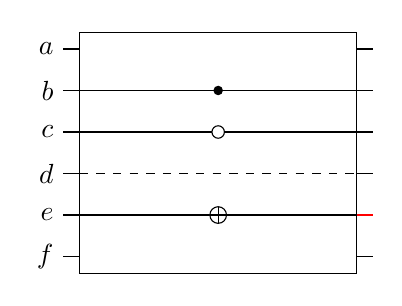
\begin{tikzpicture}[scale=1.000000,x=1pt,y=1pt]
\filldraw[color=white] (0.000000, -7.500000) rectangle (112.000000, 82.500000);
% Drawing wires
% Line 1: a W a
\draw[color=black] (0.000000,75.000000) -- (112.000000,75.000000);
\draw[color=black] (0.000000,75.000000) node[left] {$a$};
% Line 2: b W b
\draw[color=black] (0.000000,60.000000) -- (112.000000,60.000000);
\draw[color=black] (0.000000,60.000000) node[left] {$b$};
% Line 3: c W c
\draw[color=black] (0.000000,45.000000) -- (112.000000,45.000000);
\draw[color=black] (0.000000,45.000000) node[left] {$c$};
% Line 4: d W d
\draw[color=black] (0.000000,30.000000) -- (112.000000,30.000000);
\draw[color=black] (0.000000,30.000000) node[left] {$d$};
% Line 5: e W e
\draw[color=black] (0.000000,15.000000) -- (56.000000,15.000000);
\draw[color=red] (56.000000,15.000000) -- (112.000000,15.000000);
\draw[color=black] (0.000000,15.000000) node[left] {$e$};
% Line 6: f W f
\draw[color=black] (0.000000,0.000000) -- (112.000000,0.000000);
\draw[color=black] (0.000000,0.000000) node[left] {$f$};
% Done with wires; drawing gates
% Line 8: a f G {} b -c +e:color=red width=100
\draw (56.000000,75.000000) -- (56.000000,0.000000);
\begin{scope}
\draw[fill=white] (56.000000, 37.500000) +(-45.000000:70.710678pt and 61.518290pt) -- +(45.000000:70.710678pt and 61.518290pt) -- +(135.000000:70.710678pt and 61.518290pt) -- +(225.000000:70.710678pt and 61.518290pt) -- cycle;
\clip (56.000000, 37.500000) +(-45.000000:70.710678pt and 61.518290pt) -- +(45.000000:70.710678pt and 61.518290pt) -- +(135.000000:70.710678pt and 61.518290pt) -- +(225.000000:70.710678pt and 61.518290pt) -- cycle;
\draw (56.000000, 37.500000) node {{}};
\end{scope}
\draw[color=black] (6.000000, 60.000000) -- (106.000000, 60.000000);
\draw[color=black] (6.000000, 45.000000) -- (106.000000, 45.000000);
\draw[color=black,dashed] (6.000000, 30.000000) -- (106.000000, 30.000000);
\draw[color=black] (6.000000, 15.000000) -- (106.000000, 15.000000);
\filldraw (56.000000, 60.000000) circle(1.500000pt);
\draw[fill=white] (56.000000, 45.000000) circle(2.250000pt);
\begin{scope}
\draw[fill=white] (56.000000, 15.000000) circle(3.000000pt);
\clip (56.000000, 15.000000) circle(3.000000pt);
\draw (53.000000, 15.000000) -- (59.000000, 15.000000);
\draw (56.000000, 12.000000) -- (56.000000, 18.000000);
\end{scope}
% Done with gates; drawing ending labels
% Done with ending labels; drawing cut lines and comments
% Done with comments
\end{tikzpicture}

\end{figure}

\SaveVerb{name}|tmp|
\begin{figure}[ht]
\caption{\protect\UseVerb{name}}
%! \usetikzlibrary{decorations.pathreplacing,decorations.pathmorphing}
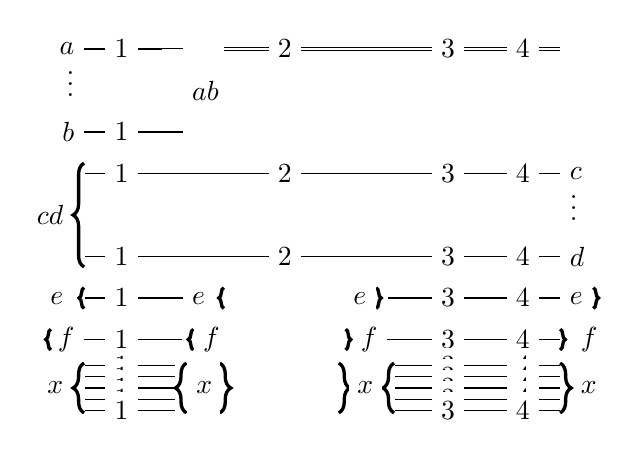
\begin{tikzpicture}[scale=1.000000,x=1pt,y=1pt]
\filldraw[color=white] (0.000000, -2.000000) rectangle (172.000000, 138.000000);
% Drawing wires
% Line 1: a W a
\draw[color=black] (0.000000,130.500000) -- (43.000000,130.500000);
\draw[color=black] (43.000000,130.000000) -- (172.000000,130.000000);
\draw[color=black] (43.000000,131.000000) -- (172.000000,131.000000);
\draw[color=black] (0.000000,130.500000) node[left] {$a$};
% Line 4: c ...cd d W cd<
\draw[color=black] (0.000000,85.500000) -- (172.000000,85.500000);
%   Deferring wire label at (0.000000,85.500000)
% Line 2: ...a W
\draw[color=black] (0.000000,115.500000) node[anchor=mid east] {$\vdots$};
% Line 6: e W e< e< e> e>
\draw[color=black] (0.000000,40.500000) -- (43.000000,40.500000);
\draw[color=black] (102.000000,40.500000) -- (172.000000,40.500000);
\filldraw[color=white,fill=white] (0.000000,36.750000) rectangle (-4.000000,44.250000);
\draw[decorate,decoration={brace,amplitude = 1.875000pt},very thick] (0.000000,36.750000) -- (0.000000,44.250000);
\draw[color=black] (-4.000000,40.500000) node[left] {$e$};
% Line 4: c ...cd d W cd<
\draw[color=black] (0.000000,55.500000) -- (172.000000,55.500000);
%   Deferring wire label at (0.000000,55.500000)
% Line 9: g h i j k W x< <x> >x< >x breadth=4
\draw[color=black] (0.000000,16.000000) -- (43.000000,16.000000);
\draw[color=black] (102.000000,16.000000) -- (172.000000,16.000000);
%   Deferring wire label at (0.000000,16.000000)
% Line 7: f W <f <f >f >f
\draw[color=black] (0.000000,25.500000) -- (43.000000,25.500000);
\draw[color=black] (102.000000,25.500000) -- (172.000000,25.500000);
\filldraw[color=white,fill=white] (-16.000000,21.750000) rectangle (-12.000000,29.250000);
\draw[decorate,decoration={brace,amplitude = 1.875000pt},very thick] (-12.000000,21.750000) -- (-12.000000,29.250000);
\draw[color=black] (0.000000,25.500000) node[left] {$f$};
% Line 9: g h i j k W x< <x> >x< >x breadth=4
\draw[color=black] (0.000000,8.000000) -- (43.000000,8.000000);
\draw[color=black] (102.000000,8.000000) -- (172.000000,8.000000);
%   Deferring wire label at (0.000000,8.000000)
% Line 9: g h i j k W x< <x> >x< >x breadth=4
\draw[color=black] (0.000000,12.000000) -- (43.000000,12.000000);
\draw[color=black] (102.000000,12.000000) -- (172.000000,12.000000);
%   Deferring wire label at (0.000000,12.000000)
% Line 9: g h i j k W x< <x> >x< >x breadth=4
\draw[color=black] (0.000000,0.000000) -- (43.000000,0.000000);
\draw[color=black] (102.000000,0.000000) -- (172.000000,0.000000);
%   Deferring wire label at (0.000000,0.000000)
% Line 9: g h i j k W x< <x> >x< >x breadth=4
\draw[color=black] (0.000000,4.000000) -- (43.000000,4.000000);
\draw[color=black] (102.000000,4.000000) -- (172.000000,4.000000);
\filldraw[color=white,fill=white] (0.000000,-1.000000) rectangle (-4.000000,17.000000);
\draw[decorate,decoration={brace,amplitude = 4.000000pt},very thick] (0.000000,-1.000000) -- (0.000000,17.000000);
\draw[color=black] (-4.000000,8.000000) node[left] {$x$};
% Line 4: c ...cd d W cd<
\filldraw[color=white,fill=white] (0.000000,51.750000) rectangle (-4.000000,89.250000);
\draw[decorate,decoration={brace,amplitude = 4.000000pt},very thick] (0.000000,51.750000) -- (0.000000,89.250000);
\draw[color=black] (-4.000000,70.500000) node[left] {$cd$};
% Line 3: b W b
\draw[color=black] (0.000000,100.500000) -- (43.000000,100.500000);
\draw[color=black] (0.000000,100.500000) node[left] {$b$};
% Done with wires; drawing gates
% Line 19: LABEL 1
\draw[color=black] (13.500000, 130.500000) node [fill=white] {$1$};
\draw[color=black] (13.500000, 100.500000) node [fill=white] {$1$};
\draw[color=black] (13.500000, 85.500000) node [fill=white] {$1$};
\draw[color=black] (13.500000, 55.500000) node [fill=white] {$1$};
\draw[color=black] (13.500000, 40.500000) node [fill=white] {$1$};
\draw[color=black] (13.500000, 25.500000) node [fill=white] {$1$};
\draw[color=black] (13.500000, 16.000000) node [fill=white] {$1$};
\draw[color=black] (13.500000, 12.000000) node [fill=white] {$1$};
\draw[color=black] (13.500000, 8.000000) node [fill=white] {$1$};
\draw[color=black] (13.500000, 4.000000) node [fill=white] {$1$};
\draw[color=black] (13.500000, 0.000000) node [fill=white] {$1$};
% Line 20: e f END
\filldraw[color=white,fill=white] (50.500000,36.750000) rectangle (46.500000,44.250000);
\draw[decorate,decoration={brace,amplitude = 1.875000pt},very thick] (50.500000,36.750000) -- (50.500000,44.250000);
\draw[color=black] (35.500000,40.500000) node[fill=white,right,minimum height=15.000000pt,minimum width=11.000000pt,inner sep=0pt] {\phantom{$e$}};
\draw[color=black] (35.500000,40.500000) node[right] {$e$};
\filldraw[color=white,fill=white] (35.500000,21.750000) rectangle (39.500000,29.250000);
\draw[decorate,decoration={brace,amplitude = 1.875000pt},very thick] (39.500000,21.750000) -- (39.500000,29.250000);
\draw[color=black] (39.500000,25.500000) node[fill=white,right,minimum height=15.000000pt,minimum width=11.000000pt,inner sep=0pt] {\phantom{$f$}};
\draw[color=black] (39.500000,25.500000) node[right] {$f$};
% Line 21: g h i j k END length=20
%   Deferring wire label at (33.000000,16.000000)
%   Deferring wire label at (33.000000,12.000000)
%   Deferring wire label at (33.000000,8.000000)
%   Deferring wire label at (33.000000,4.000000)
\filldraw[color=white,fill=white] (33.000000,-1.000000) rectangle (37.000000,17.000000);
\draw[decorate,decoration={brace,amplitude = 4.000000pt},very thick] (37.000000,-1.000000) -- (37.000000,17.000000);
\filldraw[color=white,fill=white] (53.000000,-1.000000) rectangle (49.000000,17.000000);
\draw[decorate,decoration={brace,mirror,amplitude = 4.000000pt},very thick] (49.000000,-1.000000) -- (49.000000,17.000000);
\draw[color=black] (37.000000,8.000000) node[fill=white,right,minimum height=20.000000pt,minimum width=12.000000pt,inner sep=0pt] {\phantom{$x$}};
\draw[color=black] (37.000000,8.000000) node[right] {$x$};
% Line 22: a ...a b END a:cwire
%   Deferring wire label at (35.500000,130.500000)
\draw[color=black] (35.500000,115.500000) node[fill=white,right,minimum height=15.000000pt,minimum width=15.000000pt,anchor = base,inner sep=0pt] {\phantom{$\;\vdots\;$}};
\draw[color=black] (35.500000,115.500000) node[anchor=mid west] {$\vdots$};
\draw[color=black] (35.500000,115.500000) node[fill=white,right,minimum height=45.000000pt,minimum width=15.000000pt,inner sep=0pt] {\phantom{$ab$}};
\draw[color=black] (35.500000,115.500000) node[right] {$ab$};
% Line 23: LABEL 2
\draw[color=black] (72.500000, 130.500000) node [fill=white] {$2$};
\draw[color=black] (72.500000, 85.500000) node [fill=white] {$2$};
\draw[color=black] (72.500000, 55.500000) node [fill=white] {$2$};
% Line 24: e f START
\filldraw[color=white,fill=white] (109.500000,36.750000) rectangle (105.500000,44.250000);
\draw[decorate,decoration={brace,mirror,amplitude = 1.875000pt},very thick] (105.500000,36.750000) -- (105.500000,44.250000);
\draw[color=black] (105.500000,40.500000) node[fill=white,left,minimum height=15.000000pt,minimum width=11.000000pt,inner sep=0pt] {\phantom{$e$}};
\draw[color=black] (105.500000,40.500000) node[left] {$e$};
\filldraw[color=white,fill=white] (94.500000,21.750000) rectangle (98.500000,29.250000);
\draw[decorate,decoration={brace,mirror,amplitude = 1.875000pt},very thick] (94.500000,21.750000) -- (94.500000,29.250000);
\draw[color=black] (109.500000,25.500000) node[fill=white,left,minimum height=15.000000pt,minimum width=11.000000pt,inner sep=0pt] {\phantom{$f$}};
\draw[color=black] (109.500000,25.500000) node[left] {$f$};
% Line 25: g h i j k START length=20
%   Deferring wire label at (112.000000,16.000000)
%   Deferring wire label at (112.000000,12.000000)
%   Deferring wire label at (112.000000,8.000000)
%   Deferring wire label at (112.000000,4.000000)
\filldraw[color=white,fill=white] (92.000000,-1.000000) rectangle (96.000000,17.000000);
\draw[decorate,decoration={brace,mirror,amplitude = 4.000000pt},very thick] (92.000000,-1.000000) -- (92.000000,17.000000);
\filldraw[color=white,fill=white] (112.000000,-1.000000) rectangle (108.000000,17.000000);
\draw[decorate,decoration={brace,amplitude = 4.000000pt},very thick] (112.000000,-1.000000) -- (112.000000,17.000000);
\draw[color=black] (108.000000,8.000000) node[fill=white,left,minimum height=20.000000pt,minimum width=12.000000pt,inner sep=0pt] {\phantom{$x$}};
\draw[color=black] (108.000000,8.000000) node[left] {$x$};
% Line 26: LABEL 3
\draw[color=black] (131.500000, 130.500000) node [fill=white] {$3$};
\draw[color=black] (131.500000, 85.500000) node [fill=white] {$3$};
\draw[color=black] (131.500000, 55.500000) node [fill=white] {$3$};
\draw[color=black] (131.500000, 40.500000) node [fill=white] {$3$};
\draw[color=black] (131.500000, 25.500000) node [fill=white] {$3$};
\draw[color=black] (131.500000, 16.000000) node [fill=white] {$3$};
\draw[color=black] (131.500000, 12.000000) node [fill=white] {$3$};
\draw[color=black] (131.500000, 8.000000) node [fill=white] {$3$};
\draw[color=black] (131.500000, 4.000000) node [fill=white] {$3$};
\draw[color=black] (131.500000, 0.000000) node [fill=white] {$3$};
% Line 27: LABEL 4
\draw[color=black] (158.500000, 130.500000) node [fill=white] {$4$};
\draw[color=black] (158.500000, 85.500000) node [fill=white] {$4$};
\draw[color=black] (158.500000, 55.500000) node [fill=white] {$4$};
\draw[color=black] (158.500000, 40.500000) node [fill=white] {$4$};
\draw[color=black] (158.500000, 25.500000) node [fill=white] {$4$};
\draw[color=black] (158.500000, 16.000000) node [fill=white] {$4$};
\draw[color=black] (158.500000, 12.000000) node [fill=white] {$4$};
\draw[color=black] (158.500000, 8.000000) node [fill=white] {$4$};
\draw[color=black] (158.500000, 4.000000) node [fill=white] {$4$};
\draw[color=black] (158.500000, 0.000000) node [fill=white] {$4$};
% Done with gates; drawing ending labels
\draw[color=black] (172.000000,85.500000) node[right] {$c$};
\filldraw[color=white,fill=white] (188.000000,36.750000) rectangle (184.000000,44.250000);
\draw[decorate,decoration={brace,mirror,amplitude = 1.875000pt},very thick] (184.000000,36.750000) -- (184.000000,44.250000);
\draw[color=black] (172.000000,40.500000) node[right] {$e$};
\draw[color=black] (172.000000,55.500000) node[right] {$d$};
%   Deferring wire label at (172.000000,16.000000)
\filldraw[color=white,fill=white] (172.000000,21.750000) rectangle (176.000000,29.250000);
\draw[decorate,decoration={brace,mirror,amplitude = 1.875000pt},very thick] (172.000000,21.750000) -- (172.000000,29.250000);
\draw[color=black] (176.000000,25.500000) node[right] {$f$};
%   Deferring wire label at (172.000000,8.000000)
%   Deferring wire label at (172.000000,12.000000)
%   Deferring wire label at (172.000000,0.000000)
\filldraw[color=white,fill=white] (172.000000,-1.000000) rectangle (176.000000,17.000000);
\draw[decorate,decoration={brace,mirror,amplitude = 4.000000pt},very thick] (172.000000,-1.000000) -- (172.000000,17.000000);
\draw[color=black] (176.000000,8.000000) node[right] {$x$};
\draw[color=black] (172.000000,70.500000) node[anchor=mid west] {$\vdots$};
% Done with ending labels; drawing cut lines and comments
% Done with comments
\end{tikzpicture}

\end{figure}

\SaveVerb{name}|wiretest|
\begin{figure}[ht]
\caption{\protect\UseVerb{name}}
%! \usetikzlibrary{decorations.pathreplacing,decorations.pathmorphing}
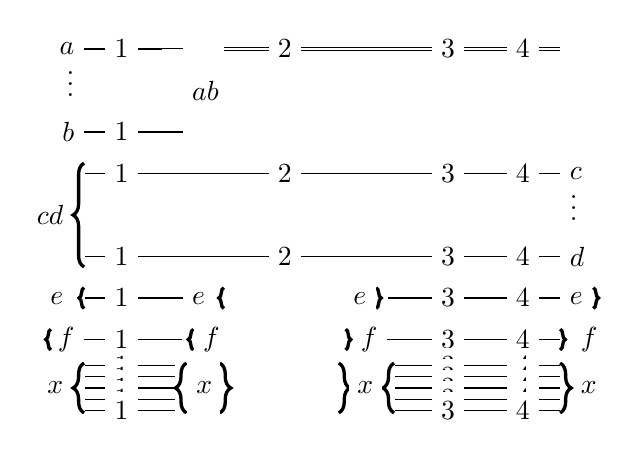
\begin{tikzpicture}[scale=1.000000,x=1pt,y=1pt]
\filldraw[color=white] (0.000000, -2.000000) rectangle (172.000000, 138.000000);
% Drawing wires
% Line 1: a W a
\draw[color=black] (0.000000,130.500000) -- (43.000000,130.500000);
\draw[color=black] (43.000000,130.000000) -- (172.000000,130.000000);
\draw[color=black] (43.000000,131.000000) -- (172.000000,131.000000);
\draw[color=black] (0.000000,130.500000) node[left] {$a$};
% Line 2: ...a W
\draw[color=black] (0.000000,115.500000) node[anchor=mid east] {$\vdots$};
% Line 3: b W b
\draw[color=black] (0.000000,100.500000) -- (43.000000,100.500000);
\draw[color=black] (0.000000,100.500000) node[left] {$b$};
% Line 4: c ...cd d W cd<
\draw[color=black] (0.000000,85.500000) -- (172.000000,85.500000);
%   Deferring wire label at (0.000000,85.500000)
% Line 4: c ...cd d W cd<
%   Deferring wire label at (0.000000,70.500000)
% Line 4: c ...cd d W cd<
\draw[color=black] (0.000000,55.500000) -- (172.000000,55.500000);
\filldraw[color=white,fill=white] (0.000000,51.750000) rectangle (-4.000000,89.250000);
\draw[decorate,decoration={brace,amplitude = 4.000000pt},very thick] (0.000000,51.750000) -- (0.000000,89.250000);
\draw[color=black] (-4.000000,70.500000) node[left] {$cd$};
% Line 6: e W e< e< e> e>
\draw[color=black] (0.000000,40.500000) -- (43.000000,40.500000);
\draw[color=black] (102.000000,40.500000) -- (172.000000,40.500000);
\filldraw[color=white,fill=white] (0.000000,36.750000) rectangle (-4.000000,44.250000);
\draw[decorate,decoration={brace,amplitude = 1.875000pt},very thick] (0.000000,36.750000) -- (0.000000,44.250000);
\draw[color=black] (-4.000000,40.500000) node[left] {$e$};
% Line 7: f W <f <f >f >f
\draw[color=black] (0.000000,25.500000) -- (43.000000,25.500000);
\draw[color=black] (102.000000,25.500000) -- (172.000000,25.500000);
\filldraw[color=white,fill=white] (-16.000000,21.750000) rectangle (-12.000000,29.250000);
\draw[decorate,decoration={brace,amplitude = 1.875000pt},very thick] (-12.000000,21.750000) -- (-12.000000,29.250000);
\draw[color=black] (0.000000,25.500000) node[left] {$f$};
% Line 9: g h i j k W x< <x> >x< >x breadth=4
\draw[color=black] (0.000000,16.000000) -- (43.000000,16.000000);
\draw[color=black] (102.000000,16.000000) -- (172.000000,16.000000);
%   Deferring wire label at (0.000000,16.000000)
% Line 9: g h i j k W x< <x> >x< >x breadth=4
\draw[color=black] (0.000000,12.000000) -- (43.000000,12.000000);
\draw[color=black] (102.000000,12.000000) -- (172.000000,12.000000);
%   Deferring wire label at (0.000000,12.000000)
% Line 9: g h i j k W x< <x> >x< >x breadth=4
\draw[color=black] (0.000000,8.000000) -- (43.000000,8.000000);
\draw[color=black] (102.000000,8.000000) -- (172.000000,8.000000);
%   Deferring wire label at (0.000000,8.000000)
% Line 9: g h i j k W x< <x> >x< >x breadth=4
\draw[color=black] (0.000000,4.000000) -- (43.000000,4.000000);
\draw[color=black] (102.000000,4.000000) -- (172.000000,4.000000);
%   Deferring wire label at (0.000000,4.000000)
% Line 9: g h i j k W x< <x> >x< >x breadth=4
\draw[color=black] (0.000000,0.000000) -- (43.000000,0.000000);
\draw[color=black] (102.000000,0.000000) -- (172.000000,0.000000);
\filldraw[color=white,fill=white] (0.000000,-1.000000) rectangle (-4.000000,17.000000);
\draw[decorate,decoration={brace,amplitude = 4.000000pt},very thick] (0.000000,-1.000000) -- (0.000000,17.000000);
\draw[color=black] (-4.000000,8.000000) node[left] {$x$};
% Done with wires; drawing gates
% Line 19: LABEL 1
\draw[color=black] (13.500000, 130.500000) node [fill=white] {$1$};
\draw[color=black] (13.500000, 100.500000) node [fill=white] {$1$};
\draw[color=black] (13.500000, 85.500000) node [fill=white] {$1$};
\draw[color=black] (13.500000, 55.500000) node [fill=white] {$1$};
\draw[color=black] (13.500000, 40.500000) node [fill=white] {$1$};
\draw[color=black] (13.500000, 25.500000) node [fill=white] {$1$};
\draw[color=black] (13.500000, 16.000000) node [fill=white] {$1$};
\draw[color=black] (13.500000, 12.000000) node [fill=white] {$1$};
\draw[color=black] (13.500000, 8.000000) node [fill=white] {$1$};
\draw[color=black] (13.500000, 4.000000) node [fill=white] {$1$};
\draw[color=black] (13.500000, 0.000000) node [fill=white] {$1$};
% Line 20: e f END
\filldraw[color=white,fill=white] (50.500000,36.750000) rectangle (46.500000,44.250000);
\draw[decorate,decoration={brace,amplitude = 1.875000pt},very thick] (50.500000,36.750000) -- (50.500000,44.250000);
\draw[color=black] (35.500000,40.500000) node[fill=white,right,minimum height=15.000000pt,minimum width=11.000000pt,inner sep=0pt] {\phantom{$e$}};
\draw[color=black] (35.500000,40.500000) node[right] {$e$};
\filldraw[color=white,fill=white] (35.500000,21.750000) rectangle (39.500000,29.250000);
\draw[decorate,decoration={brace,amplitude = 1.875000pt},very thick] (39.500000,21.750000) -- (39.500000,29.250000);
\draw[color=black] (39.500000,25.500000) node[fill=white,right,minimum height=15.000000pt,minimum width=11.000000pt,inner sep=0pt] {\phantom{$f$}};
\draw[color=black] (39.500000,25.500000) node[right] {$f$};
% Line 21: g h i j k END length=20
%   Deferring wire label at (33.000000,16.000000)
%   Deferring wire label at (33.000000,12.000000)
%   Deferring wire label at (33.000000,8.000000)
%   Deferring wire label at (33.000000,4.000000)
\filldraw[color=white,fill=white] (33.000000,-1.000000) rectangle (37.000000,17.000000);
\draw[decorate,decoration={brace,amplitude = 4.000000pt},very thick] (37.000000,-1.000000) -- (37.000000,17.000000);
\filldraw[color=white,fill=white] (53.000000,-1.000000) rectangle (49.000000,17.000000);
\draw[decorate,decoration={brace,mirror,amplitude = 4.000000pt},very thick] (49.000000,-1.000000) -- (49.000000,17.000000);
\draw[color=black] (37.000000,8.000000) node[fill=white,right,minimum height=20.000000pt,minimum width=12.000000pt,inner sep=0pt] {\phantom{$x$}};
\draw[color=black] (37.000000,8.000000) node[right] {$x$};
% Line 22: a ...a b END a:cwire
%   Deferring wire label at (35.500000,130.500000)
\draw[color=black] (35.500000,115.500000) node[fill=white,right,minimum height=15.000000pt,minimum width=15.000000pt,anchor = base,inner sep=0pt] {\phantom{$\;\vdots\;$}};
\draw[color=black] (35.500000,115.500000) node[anchor=mid west] {$\vdots$};
\draw[color=black] (35.500000,115.500000) node[fill=white,right,minimum height=45.000000pt,minimum width=15.000000pt,inner sep=0pt] {\phantom{$ab$}};
\draw[color=black] (35.500000,115.500000) node[right] {$ab$};
% Line 23: LABEL 2
\draw[color=black] (72.500000, 130.500000) node [fill=white] {$2$};
\draw[color=black] (72.500000, 85.500000) node [fill=white] {$2$};
\draw[color=black] (72.500000, 55.500000) node [fill=white] {$2$};
% Line 24: e f START
\filldraw[color=white,fill=white] (109.500000,36.750000) rectangle (105.500000,44.250000);
\draw[decorate,decoration={brace,mirror,amplitude = 1.875000pt},very thick] (105.500000,36.750000) -- (105.500000,44.250000);
\draw[color=black] (105.500000,40.500000) node[fill=white,left,minimum height=15.000000pt,minimum width=11.000000pt,inner sep=0pt] {\phantom{$e$}};
\draw[color=black] (105.500000,40.500000) node[left] {$e$};
\filldraw[color=white,fill=white] (94.500000,21.750000) rectangle (98.500000,29.250000);
\draw[decorate,decoration={brace,mirror,amplitude = 1.875000pt},very thick] (94.500000,21.750000) -- (94.500000,29.250000);
\draw[color=black] (109.500000,25.500000) node[fill=white,left,minimum height=15.000000pt,minimum width=11.000000pt,inner sep=0pt] {\phantom{$f$}};
\draw[color=black] (109.500000,25.500000) node[left] {$f$};
% Line 25: g h i j k START length=20
%   Deferring wire label at (112.000000,16.000000)
%   Deferring wire label at (112.000000,12.000000)
%   Deferring wire label at (112.000000,8.000000)
%   Deferring wire label at (112.000000,4.000000)
\filldraw[color=white,fill=white] (92.000000,-1.000000) rectangle (96.000000,17.000000);
\draw[decorate,decoration={brace,mirror,amplitude = 4.000000pt},very thick] (92.000000,-1.000000) -- (92.000000,17.000000);
\filldraw[color=white,fill=white] (112.000000,-1.000000) rectangle (108.000000,17.000000);
\draw[decorate,decoration={brace,amplitude = 4.000000pt},very thick] (112.000000,-1.000000) -- (112.000000,17.000000);
\draw[color=black] (108.000000,8.000000) node[fill=white,left,minimum height=20.000000pt,minimum width=12.000000pt,inner sep=0pt] {\phantom{$x$}};
\draw[color=black] (108.000000,8.000000) node[left] {$x$};
% Line 26: LABEL 3
\draw[color=black] (131.500000, 130.500000) node [fill=white] {$3$};
\draw[color=black] (131.500000, 85.500000) node [fill=white] {$3$};
\draw[color=black] (131.500000, 55.500000) node [fill=white] {$3$};
\draw[color=black] (131.500000, 40.500000) node [fill=white] {$3$};
\draw[color=black] (131.500000, 25.500000) node [fill=white] {$3$};
\draw[color=black] (131.500000, 16.000000) node [fill=white] {$3$};
\draw[color=black] (131.500000, 12.000000) node [fill=white] {$3$};
\draw[color=black] (131.500000, 8.000000) node [fill=white] {$3$};
\draw[color=black] (131.500000, 4.000000) node [fill=white] {$3$};
\draw[color=black] (131.500000, 0.000000) node [fill=white] {$3$};
% Line 27: LABEL 4
\draw[color=black] (158.500000, 130.500000) node [fill=white] {$4$};
\draw[color=black] (158.500000, 85.500000) node [fill=white] {$4$};
\draw[color=black] (158.500000, 55.500000) node [fill=white] {$4$};
\draw[color=black] (158.500000, 40.500000) node [fill=white] {$4$};
\draw[color=black] (158.500000, 25.500000) node [fill=white] {$4$};
\draw[color=black] (158.500000, 16.000000) node [fill=white] {$4$};
\draw[color=black] (158.500000, 12.000000) node [fill=white] {$4$};
\draw[color=black] (158.500000, 8.000000) node [fill=white] {$4$};
\draw[color=black] (158.500000, 4.000000) node [fill=white] {$4$};
\draw[color=black] (158.500000, 0.000000) node [fill=white] {$4$};
% Done with gates; drawing ending labels
\draw[color=black] (172.000000,85.500000) node[right] {$c$};
\draw[color=black] (172.000000,70.500000) node[anchor=mid west] {$\vdots$};
\draw[color=black] (172.000000,55.500000) node[right] {$d$};
\filldraw[color=white,fill=white] (188.000000,36.750000) rectangle (184.000000,44.250000);
\draw[decorate,decoration={brace,mirror,amplitude = 1.875000pt},very thick] (184.000000,36.750000) -- (184.000000,44.250000);
\draw[color=black] (172.000000,40.500000) node[right] {$e$};
\filldraw[color=white,fill=white] (172.000000,21.750000) rectangle (176.000000,29.250000);
\draw[decorate,decoration={brace,mirror,amplitude = 1.875000pt},very thick] (172.000000,21.750000) -- (172.000000,29.250000);
\draw[color=black] (176.000000,25.500000) node[right] {$f$};
%   Deferring wire label at (172.000000,16.000000)
%   Deferring wire label at (172.000000,12.000000)
%   Deferring wire label at (172.000000,8.000000)
%   Deferring wire label at (172.000000,4.000000)
\filldraw[color=white,fill=white] (172.000000,-1.000000) rectangle (176.000000,17.000000);
\draw[decorate,decoration={brace,mirror,amplitude = 4.000000pt},very thick] (172.000000,-1.000000) -- (172.000000,17.000000);
\draw[color=black] (176.000000,8.000000) node[right] {$x$};
% Done with ending labels; drawing cut lines and comments
% Done with comments
\end{tikzpicture}

\end{figure}
\clearpage

\end{document}
